% !TeX program = xelatex
% 复用同仓库 Irodov 专区 ElegantBook 类；原书版权归权利人。
\documentclass[lang=cn,color=blue,11pt]{elegantbook}
\usepackage{amsmath,amssymb,mathtools,bm}
\usepackage{tikz}
\usetikzlibrary{arrows.meta,calc}
\newcommand{\sourceproblem}[3]{\par\medskip\noindent\textbf{\large 教材习题 #1}\hfill{\small 书内第 #2 页，PDF第 #3 页}\par\nobreak\smallskip}
\newcommand{\problemtext}{\par\noindent\textbf{【题意整理】}\quad}
\newcommand{\workings}{\par\smallskip\noindent\textbf{【推导与解析】}\quad}
\newcommand{\crosscheck}{\par\smallskip\noindent\textbf{【核验】}\quad}
\title{大学物理三校习题研究性详解}
\subtitle{天津理工大学、华中科技大学、常州工学院}
\author{独立题解与 LaTeX 排版：三千弱水}
\date{2026年11月24日}
\version{0.46}
\begin{document}
\maketitle
\frontmatter
\chapter*{编辑说明}
按原书编号与双页码记录。题意独立概述，推导及核验独立撰写；不上传底本、原书扫描图或整页复制。三册独立统计，累计1598个题号，三册章末习题均已覆盖至末题；其中有部分解析及历史疑点。第46批全量源码结构检查通过，累计独立二轮复核351个题号（含条件疑点），全量学术终审及PDF编译尚待完成。公开再版前须核验授权。
\tableofcontents
\mainmatter
\chapter{天津理工大学《大学物理同步训练》（第3版）}
\section{质点运动学}
\sourceproblem{选择1}{1}{7}
\problemtext 判断一维运动何时趋向原点。
\workings 到原点距离为 $|x|$；在 $x\ne0$ 时，距离减小等价于 $x\dot x<0$，即 $\mathrm d(x^2)/\mathrm dt<0$，选 C。
\crosscheck $x>0$ 时须 $\dot x<0$，$x<0$ 时须 $\dot x>0$；在原点不能称为正在趋近原点。
\sourceproblem{选择2}{1}{7}
\problemtext 识别瞬时速率的等价表达式。
\workings $\bm v=\mathrm d\bm r/\mathrm dt$，$v=|\bm v|=\mathrm ds/\mathrm dt=\sqrt{\dot x^2+\dot y^2+\dot z^2}$，也等于速度坐标分量所构成矢量的模。故原式(2)(3)(4)(5)正确，选 B。
\crosscheck 速度矢量本身不是其大小；弧长 $s$ 为累计路程。
\sourceproblem{选择3}{1}{7}
\problemtext $x=5+3t^2-t^3$（SI），判断运动方向与速率变化。
\workings $v=3t(2-t)$，$a=6(1-t)$。$0<t<1$ 时二者均正；$1<t<2$ 时 $v>0,a<0$；$t>2$ 时二者均负。故选 B。
\crosscheck 速率增减由 $va$ 的符号确定，$t=2$ 是速度换向点。
\sourceproblem{选择4}{1}{7}
\problemtext $\bm r=(3t^2+2)\bm i+6t^2\bm j$，判别轨迹及速率。
\workings 消去 $t$ 得 $y=2(x-2)$，$x\ge2$；$\bm v=6t\bm i+12t\bm j$，速率为 $6\sqrt5|t|$。选 B（变速直线）。
\crosscheck 加速度 $6\bm i+12\bm j$ 恒定；轨迹为直线上的半直线。
\sourceproblem{选择5}{1}{7}
\problemtext $x=t^2-40t$，求 $t_1$ 至 $t_2$ 的平均速度。
\workings 当 $t_2>t_1$ 时，
\[
\bar v=\frac{(t_2^2-t_1^2)-40(t_2-t_1)}{t_2-t_1}=t_1+t_2-40.
\]
选 A。
\crosscheck $t_2\to t_1$ 时趋于瞬时速度 $2t_1-40$，不可把平均速度当平均速率。

\section{质点动力学}
\sourceproblem{选择1}{5}{11}
\problemtext 判断保守力负功、闭路功及作用反作用力的总功三项命题。
\workings 保守力功 $W_c=-\Delta U$，故负功使势能增加；闭路积分 $\oint\bm F_c\cdot\mathrm d\bm r=0$；作用反作用力作用于不同物体，其总功为 $\int\bm F_{12}\cdot(\mathrm d\bm r_1-\mathrm d\bm r_2)$，一般非零。仅第二项成立，选C。
\crosscheck 例如滑动摩擦力对两个接触物体的总功为负，不能由力的矢量和为零推出总功为零。
\sourceproblem{选择2}{5}{11}
\problemtext 判断系统机械能守恒的充分条件。
\workings 对固定组成系统，$\Delta(K+U)=W_{\rm ext}+W_{\rm nc,int}$，其中 $U$ 只包含内保守力势能；外力及非保守内力均不做功时机械能守恒，选C。
\crosscheck 合外力为零不能保证各外力总功为零；内摩擦也能改变机械能。更一般的充分条件是两类功的总和为零。
\sourceproblem{填空1}{5}{11}
\problemtext 从10米深井匀速提升1千克的桶，初装水10千克，每升高1米漏水0.2千克，求人做功。
\workings 令提升高度 $z$，桶及剩余水质量 $M(z)=11-0.2z$（SI）。忽略漏水相对桶的竖向动量通量反作用，
\[
W=\int_0^{10}(11-0.2z)g\,\mathrm dz=100g\,\mathrm J.
\]
取 $g=9.8\,\mathrm{m/s^2}$ 得 $980\,\mathrm J$。
\crosscheck 平均质量为10千克；若漏出水流具有不可忽略的相对竖向速度，需另给流动模型才能计算拉力。
\sourceproblem{填空2}{5}{11}
\problemtext $x=t^2$（SI），阻力大小为 $kv^2$，$k=0.5$，求 $x=0$ 至 $3\,\mathrm m$ 的阻力功。
\workings 正时间域 $v=2t$，$v^2=4x$（SI），故 $W=-\int_0^3 2x\,\mathrm dx=-9\,\mathrm J$。
\crosscheck 阻力与运动方向相反，功为负；$k$ 的量纲为质量除以长度。
\sourceproblem{计算1}{6}{12}
\problemtext 质量3千克质点从静止沿正 $x$ 轴运动，$F=6t$（N），$v=t^2$（SI），求前2秒力的功。
\workings $W=\int_0^2Fv\,\mathrm dt=\int_0^2 6t^3\,\mathrm dt=24\,\mathrm J$。
\crosscheck 牛顿定律 $3\dot v=6t$ 与题设相符；动能增量 $3(4^2)/2=24\,\mathrm J$。
\sourceproblem{计算2}{6}{12}
\problemtext 非胡克弹簧准静态拉伸所需外力 $F=50x+30x^2$（SI），由1米拉到2米求外力功。
\workings
\[
W=\int_1^2(50x+30x^2)\,\mathrm dx
=[25x^2+10x^3]_1^2=145\,\mathrm J.
\]
\crosscheck 正向外力和位移同向，功为正；不使用恒定弹性系数的胡克定律公式。

\section{刚体定轴转动}
\sourceproblem{选择1}{7}{13}
\problemtext 两均质圆盘质量和厚度相同，中心轴转动惯量 $J_B>J_A$，比较密度。
\workings $J=mR^2/2$，故 $R_B>R_A$；$\rho=m/(\pi R^2h)$，因而 $\rho_A>\rho_B$，选A。
\crosscheck 固定质量、厚度时 $J\rho=m^2/(2\pi h)$ 为常量。
\sourceproblem{选择2}{7}{13}
\problemtext 等质量、等半径的两个细环，一个质量分布均匀、另一个不均匀，比较中心垂直轴惯量。
\workings 每一质量元距轴均为 $R$，$J=\int R^2\,\mathrm dm=mR^2$，故 $J_1=J_2$，选C。
\crosscheck 结论针对细环几何中心的垂直轴，不依赖质心是否位于环心。
\sourceproblem{选择3}{7}{13}
\problemtext 按图1，圆盘顺时针转动，两等大反向平行力分别沿上、下两条作用线，判断角速度变化。
\workings 两力合力为零但构成力偶；设作用线垂直间距 $d>0$，图示合力矩为顺时针，大小 $Fd$。取顺时针为正，$\dot\omega=Fd/J>0$，故 $\omega_2>\omega_1$，选C。
\crosscheck 根据原图上方力向右、下方力向左判定力矩；不可用合力为零推出合力矩为零。
\sourceproblem{选择4}{7}{13}
\problemtext 均质杆长 $L$、质量 $M$，从水平静止绕端点水平轴下摆到竖直，判断力矩、角速度、角加速度变化。
\workings 设杆下摆角 $\phi$ 从水平起算，$\tau=MgL\cos\phi/2$，$\alpha=3g\cos\phi/(2L)$，随 $\phi$ 从0到 $\pi/2$ 均减小；能量守恒 $\omega^2=3g\sin\phi/L$，角速率增大，选A。
\crosscheck 竖直最低点角加速度为零但角速率最大。
\sourceproblem{选择5}{7}{13}
\problemtext 相同滑轮A悬挂质量 $m$，B直接受恒力 $G=mg$，比较角加速度。
\workings 轮半径 $R$、惯量 $J>0$；A有 $mg-T=ma$，$TR=J a/R$，故 $\beta_A=mgR/(J+mR^2)$；B有 $\beta_B=mgR/J$，故 $\beta_A<\beta_B$，选C。
\crosscheck A的张力小于 $mg$，因此不能把悬挂重物等同于恒拉力。
\sourceproblem{选择6}{8}{14}
\problemtext 图4中左侧 $m_1$ 小于右侧 $m_2$，滑轮某刻逆时针转动，比较绳两侧张力。
\workings 取右侧向下为正，$a=(m_2-m_1)g/(m_1+m_2+J/R^2)>0$。轮的角加速度为顺时针，$T_2-T_1=Ja/R^2>0$，故右侧张力较大，选C。
\crosscheck 当前逆时针角速度与顺时针角加速度并不矛盾；题设有惯量的轮两侧张力不等。
\sourceproblem{选择7}{8}{14}
\problemtext 固定光滑轴刚体受到数个合力为零的力，判断转速是否变化。
\workings 合力为零不决定轴向合力矩；$\dot\omega=\tau_z/J$。若 $\tau_z=0$ 则转速不变，否则通常改变，选D。
\crosscheck 力偶提供反例：净力为零但力矩非零。
\sourceproblem{选择8}{8}{14}
\problemtext 图5中两同质量、同速率、相向且共线的物体嵌入绕固定轴转动的圆盘，比较碰撞前后角速率。
\workings 两入射物体的轴向角动量互相抵消。短时碰撞中忽略外轴向冲量矩，$J\omega_1=(J+\Delta J)\omega_2$，其中 $\Delta J>0$，故 $\omega_2<\omega_1$（初始角速率非零），选A。
\crosscheck 不应用机械能守恒；嵌入是非弹性碰撞。
\sourceproblem{选择9}{8}{14}
\problemtext 比较杆与小球的非弹性碰撞系统A、人及自由旋转盘系统B的守恒量。
\workings 碰撞短时极限中A对轴的外冲量矩为零；B在忽略轴摩擦时外轴向力矩为零，故两者均有轴向角动量守恒。A的碰撞会耗散机械能；B可由人体内能转化为机械能。固定轴支承可给外冲量，线动量并不普遍守恒，选B。
\crosscheck A的角动量守恒只针对碰撞短时过程，非其后摆动全过程。
\sourceproblem{选择10}{8}{14}
\problemtext 自由绕固定光滑轴转动的物体热膨胀，判断角速度。
\workings 无外轴向力矩时 $J\omega$ 守恒。通常均匀各向同性热膨胀使各质量元轴距按比例增大，$J$ 增大、角速率减小，选B。
\crosscheck 若只沿轴向膨胀或材料各向异性，未必增加 $J$；原选项B采用常规径向膨胀假设。

\section{机械振动}
\sourceproblem{选择1}{12}{18}
\problemtext 比较弹跳、大角度单摆、矩形木块及球形木块的浮动，判断简谐运动。
\workings 矩形木块竖直浮动时，若保持部分浸没且水线截面积 $S$ 恒定，偏离平衡位置 $x$ 后合力为 $-\rho gSx$，故 $\ddot x=-(\rho gS/m)x$，选C。
\crosscheck 忽略阻力和流体附加质量；大角度单摆的回复力非线性，球形木块的水线面积通常变化。
\sourceproblem{选择2}{12}{18}
\problemtext 图1水平弹簧向左压缩后静止释放，右向为正，求余弦振动初相。
\workings $x(0)=-A,v(0)=0$，由 $x=A\cos(\omega t+\varphi)$ 得 $\varphi=\pi\pmod{2\pi}$，选D。
\crosscheck 初始回复力向右，初加速度为正。
\sourceproblem{选择3}{12}{18}
\problemtext 相同轻弹簧分别系不同质量及振幅的物体，比较水平、竖直振动周期。
\workings 理想线性弹簧 $T=2\pi\sqrt{m/k}$，重力只改变竖直振动的平衡位置，振幅不改变周期；仅B的质量不同，选B。
\crosscheck 质量倍增使周期乘 $\sqrt2$，并非乘2。
\sourceproblem{选择4}{12}{18}
\problemtext 从平衡点到半振幅位置的最短时间为 $t_0$，求周期。
\workings 令初速度朝向目标，$x=A\sin\omega t$，首次达到 $A/2$ 时 $\omega t_0=\pi/6$，故 $T=12t_0$，选B。
\crosscheck 最短时间小于四分之一周期。
\sourceproblem{选择5}{12}{18}
\problemtext 月面重力为地面的六分之一，同一小角度单摆周期如何变化？
\workings $T=2\pi\sqrt{l/g}$，故 $T_{\rm Moon}=\sqrt6T$，选C。
\crosscheck 摆长相同、小角近似成立；周期与质量无关。
\sourceproblem{选择6}{12}{18}
\problemtext 依据图2旋转矢量，初相 $\pi/4$、逆时针转过 $\pi t$，求振动方程。
\workings 取水平投影，$x=R\cos(\pi t+\pi/4)$，选A。
\crosscheck 初位置 $R/\sqrt2$、初速度 $-\pi R/\sqrt2$，与矢量转向一致。图在PDF19。
\sourceproblem{选择7}{12}{18}
\problemtext 依据图3，振幅10米，初位移负5米且上升，4秒处向下通过平衡点，求振动方程。
\workings 余弦初相取 $-2\pi/3$；图示首次向下过零对应相位 $\pi/2$，故 $4\omega=7\pi/6$，$\omega=7\pi/24$。$x=10\cos(7\pi t/24-2\pi/3)$（SI），选C。
\crosscheck 初速度为正，4秒处速度为负；根据PDF19图3排除多周期分支。
\sourceproblem{选择8}{13}{19}
\problemtext 图4振幅6米、周期4秒，2秒时向正方向过平衡点，求速度。
\workings $\omega=\pi/2\,\mathrm{rad/s}$，平衡点速率最大，$v(2)=A\omega=3\pi\,\mathrm{m/s}$，选A。
\crosscheck 原图从0时向负方向运动，2秒后正向过零。
\sourceproblem{选择9}{13}{19}
\problemtext 轻弹簧截成相等两段再并联，保持振动总能量不变，求新振幅。
\workings 均匀弹簧每半段劲度为 $2k$，并联为 $4k$。由 $kA^2/2=4kA'^2/2$ 得 $A'=A/2$，选A。
\crosscheck 弹簧均匀、质量忽略且满足线性关系；总能量相等是题设而非改装过程自动守恒。
\sourceproblem{选择10}{13}{19}
\problemtext 同向同频振动 $x_1=6\cos(5t+\pi/2)$、$x_2=2\cos(5t-\pi/2)$，求合振动。
\workings 两振动反相，$x=-6\sin5t+2\sin5t=-4\sin5t=4\cos(5t+\pi/2)$，选D。
\crosscheck 合振幅为差值4，频率不变。
\sourceproblem{选择11}{13}{19}
\problemtext 同频同向振动初相分别为 $\pi/3,-\pi/6$，振幅 $A_1,A_2$，求合振幅。
\workings 相差 $\pi/2$，矢量合成得 $A=\sqrt{A_1^2+A_2^2+2A_1A_2\cos(\pi/2)}=\sqrt{A_1^2+A_2^2}$，选C。
\crosscheck 任一分振幅为零时恢复另一分振幅。

\section{机械波}
\sourceproblem{选择1}{17}{23}
\problemtext 给定行波 $y=6\cos(\pi t-3\pi x+\pi/2)$（SI），判断波速与频率。
\workings $\omega=\pi,\ k=3\pi$，所以 $u=\omega/k=1/3\,\mathrm{m/s}$，$f=\omega/(2\pi)=1/2\,\mathrm{Hz}$，沿正 $x$ 传播，选B。
\crosscheck 波速是相位传播速度，不是质点横向振动速度。
\sourceproblem{选择2}{17}{23}
\problemtext 图1为正向传播的瞬时波形，判断波长及 $x=6\,\mathrm m$ 处质点运动方向。
\workings 图中相邻波峰相距8米，$x=6\,\mathrm m$ 处波形斜率为正。正向行波满足 $\partial_t y=-u\partial_x y$，故该处质点向下运动，选D。
\crosscheck 单张波形图在不知道波速时不能单独给出周期。
\sourceproblem{选择3}{17}{23}
\problemtext 图1的波速为10米每秒，求频率。
\workings $\lambda=8\,\mathrm m$，$f=u/\lambda=1.25\,\mathrm{Hz}$，选A。
\crosscheck $T=\lambda/u=0.8\,\mathrm s$，不是0.8赫兹。
\sourceproblem{选择4}{17}{23}
\problemtext 正向行波周期0.5秒、振幅1米、波长2米，原点初始处于负最大位移。
\workings $\omega=4\pi,k=\pi,\varphi_0=\pi$，故 $y=\cos(4\pi t-\pi x+\pi)$（SI）。
\crosscheck 原点初位移为负1米，速度为零；固定相位随时间向右移动。
\sourceproblem{选择5}{17}{23}
\problemtext 图2为沿负轴传播的波在 $t=T/4$ 时的波形，求原点振动初相。
\workings 图中原点位移为零、空间斜率为正。左行波满足 $\partial_t y=u\partial_x y>0$，故该时刻余弦相位为 $3\pi/2$，减去 $\omega T/4=\pi/2$ 得初相 $\pi$，选C。
\crosscheck 采用余弦初相约定；原点在初始时处于负最大位移。
\sourceproblem{选择6}{17}{23}
\problemtext 图3给定 $t=T/4$ 时的波形，求P点的振动方程。
\workings 图中振幅2厘米，右行波速20米每秒，波长按图刻度读为4米，则 $\omega=10\pi$。P处为正斜率过零点，质点向下运动；此刻余弦相位 $\pi/2$，减去 $\pi/2$ 得初相零。因此 $y_P=2\cos(10\pi t)$（cm）。
\crosscheck 若读图的P点或刻度与选项不符，应按 $y_P(t)=A\cos[\omega(t-T/4)+\phi_P]$ 重新辨识，$\cos\phi_P=y_P(T/4)/A$ 且速度符号由右行波斜率确定。本题保留读图待核标记，不强配选项。
\sourceproblem{选择7}{17}{23}
\problemtext 正向行波波长4米，图4中A至B相距5米，A的振动为 $5\cos(2\pi t+\pi)$（SI）；求B的振动。
\workings 相位滞后 $2\pi(5/4)=5\pi/2$，故 $y_B=5\cos(2\pi t+\pi/2)$（SI），选A。
\crosscheck 传播时间为 $5/u$，相位差与相应时间延迟一致；图示在PDF24。
\sourceproblem{选择8}{18}{24}
\problemtext 左行波波长 $\lambda$，比较 $x_1=\lambda,x_2=-\lambda/2$ 两点相位。
\workings 同时相位为 $\omega t+kx+\varphi$，所以 $\phi_1-\phi_2=k(3\lambda/2)=3\pi$；若反向定义相位差则为 $-3\pi$。两点反相。
\crosscheck 必须说明相位差的减法顺序；模 $2\pi$ 意义下等效为 $\pi$。
\sourceproblem{选择9}{18}{24}
\problemtext 理想弹性介质中的平面简谐行波，判断质元的动能、势能关系。
\workings 在无耗散线性一维行波模型，$w_K=\rho(\partial_t y)^2/2$，$w_U=\rho u^2(\partial_x y)^2/2$。因 $\partial_t y=\pm u\partial_x y$，二者始终相等，选D。
\crosscheck 质元在位移极值处两种能量密度同时为零，在过平衡位置时同时最大；不同于孤立弹簧振子。
\sourceproblem{选择10}{18}{24}
\problemtext 两同相相干波源相距 $\lambda/2$，图5直线外侧已知相消，判断连线上干涉。
\workings 两源外侧任一点的路程差恒为 $\lambda/2$，相位差为奇数倍 $\pi$，为相消条件；两源之间路程差连续从 $-\lambda/2$ 变到 $\lambda/2$，中点相长，不能说内部各点均相消或均相长。
\crosscheck 完全抵消还需两波在该点振幅相等；只根据相位判断增强或减弱。
\sourceproblem{选择11}{18}{24}
\problemtext 判断驻波的能量和相位命题。
\workings 理想驻波可写成 $y=2A\sin kx\cos\omega t$，相邻两波节之间 $\sin kx$ 同号，故非节点质元同相；跨过波节相位反转。选C。
\crosscheck 波节位移恒零，但介质形变能不必为零；波腹位移最大也不代表任意时刻总能量密度最大。
\sourceproblem{填空1}{18}{24}
\problemtext 行波 $y=5\cos(\pi t+4\pi x-\pi/2)$（SI），求传播方向、振幅、周期、波长和波速。
\workings 负 $x$ 方向，$A=5\,\mathrm m$，$T=2\,\mathrm s$，$\lambda=1/2\,\mathrm m$，$u=1/4\,\mathrm{m/s}$。
\crosscheck 固定相位满足 $\pi+4\pi\,\mathrm dx/\mathrm dt=0$。
\sourceproblem{填空2}{18}{24}
\problemtext 波在介质A中速率为 $v$，进入B后波长为原波长两倍，求B中波速。
\workings 静止界面两侧频率相同，$u_B=f(2\lambda_A)=2v$。
\crosscheck 波速改变由介质决定；频率由波源决定。
\sourceproblem{填空3}{18}{24}
\problemtext 图6瞬时波形给出A点向上运动，判断传播方向以及B、C、D点振动方向。
\workings A处空间斜率为负，由 $\partial_t y=-u\partial_x y$ 得波沿正 $x$ 传播。B处为正斜率，向下；C为负斜率，向上；D在波峰，瞬时速度为零，随后向下。
\crosscheck 原图D的精确位置待独立读图复核；若实际标在下降段而非峰顶，则D瞬时速度向上。严格判据为局部空间斜率而非位移正负。
\sourceproblem{填空4}{18}{24}
\problemtext $y=7\cos(3t-5x)$（SI），求 $x=-3$ 处振动式及与 $x=4$ 处的相位差。
\workings $y_{-3}=7\cos(3t+15)$，$y_4=7\cos(3t-20)$，所以 $\phi_{-3}-\phi_4=35\,\mathrm{rad}$。
\crosscheck 若要求主值，可对35弧度取模 $2\pi$；相位差符号须声明顺序。
\sourceproblem{填空5}{18}{24}
\problemtext 图7两波源初相差 $\pi$，到P距离分别为 $a,b$（$b>a$），P处相长干涉，求可取波长。
\workings 到P相位差为 $\pi\pm 2\pi(b-a)/\lambda$，相长要求为 $2n\pi$，故
\[
\lambda=\frac{2(b-a)}{2j+1},\qquad j=0,1,2,\ldots .
\]
\crosscheck 初相反相时奇数个半波长的路程差使到达相位一致；若问最长波长则取 $j=0$。
\sourceproblem{填空6}{18}{24}
\problemtext 同频平面简谐波强度之比为 $a$，求振幅之比。
\workings 在同一线性介质、同波型下 $\bar I=\rho u\omega^2A^2/2$，故 $A_1/A_2=\sqrt a$。
\crosscheck 若两介质波阻抗不同，需另乘波阻抗比的平方根，不能仅由同频推出该结果。
\sourceproblem{计算1}{19}{25}
\problemtext 左行简谐波波长6米，图8给出 $x=3\,\mathrm m$ 处振动曲线，求该点、行波及原点振动式。
\workings 由图读振幅10厘米、相邻峰值时间差约12秒，$t=0$ 处为正位移且下降；设从图确认的初相为 $\phi_3$。则
\[
y_3=10\cos(\omega t+\phi_3),\quad
y(x,t)=10\cos[\omega t+\tfrac{\pi}{3}(x-3)+\phi_3],\quad
y_0=10\cos(\omega t+\phi_3-\pi)
\]
（cm）。若峰值在 $t=10\,\mathrm s$ 且周期12秒，则 $\omega=\pi/6,\phi_3=\pi/3$（模 $2\pi$）。
\crosscheck 原图时间刻度较细，周期及初相保留条件式待复核；波长6米决定空间相位系数 $\pi/3$，不受读图时间误差影响。
\sourceproblem{计算2}{19}{25}
\problemtext 正向行波波速 $u$，图9中A位于 $x=a$、B位于 $x=3a$，A处振动 $y_A=A_0\cos\omega t$。求O、B处振动及与B同状态点。
\workings $k=\omega/u$，
\[
y(x,t)=A_0\cos[\omega t-k(x-a)],\quad
y_O=A_0\cos(\omega t+ka),\quad
y_B=A_0\cos(\omega t-2ka).
\]
与B同相且振幅相同的位置为 $x=3a+n(2\pi u/\omega)$，$n\in\mathbb Z$。
\crosscheck 同状态包括位移和速度，要求相位差为整周；若波尚未传播到某点，该点不能计入已振动区域。

\sourceproblem{计算3}{20}{26}
\problemtext 图10给定正向简谐行波初始波形，波速10米每秒，求原点振动及波动方程。
\workings 放大图10可见振幅10厘米，原点与 $x=10\,\mathrm m$ 处为同向空间过零点，故 $\lambda=10\,\mathrm m$，$k=\pi/5\,\mathrm{rad/m}$，$\omega=ku=2\pi\,\mathrm{rad/s}$。初始波形为 $y(x,0)=0.10\sin(\pi x/5)$，沿正向平移得
\[
y(x,t)=0.10\sin(\pi x/5-2\pi t),\qquad
y(0,t)=-0.10\sin(2\pi t)
\]
（SI）。
\crosscheck 原点初始空间斜率为正，故初速度为负；$y(x,t)=y(x-ut,0)$ 与传播方向一致。
\sourceproblem{计算4}{20}{26}
\problemtext 正向行波波速2米每秒、周期0.2秒、振幅3厘米，初始 $x=1\,\mathrm m$ 处位移为负最大值，求波动方程。
\workings $\lambda=uT=0.4\,\mathrm m$，$\omega=10\pi$，$k=5\pi$。令 $y=0.03\cos(10\pi t-5\pi x+\varphi)$，由 $-5\pi+\varphi\equiv\pi\pmod{2\pi}$ 得 $\varphi\equiv0$，所以
\[
y(x,t)=0.03\cos(10\pi t-5\pi x)\quad(\mathrm{SI}).
\]
\crosscheck 代入 $x=1,t=0$ 得 $-0.03\,\mathrm m$，此时质点速度为零；相位传播速率为2米每秒。

\section{真空中的静电场}
\sourceproblem{选择1}{21}{27}
\problemtext 两无限均匀带电平面A、B平行，面密度分别为 $\sigma,2\sigma$，B在右，求两面间及B右侧的有向场强。
\workings 取向右为正，单无限平面两侧场强的法向分量分别为 $\pm\sigma/(2\varepsilon_0)$。叠加得 $E_{\rm between}=-\sigma/(2\varepsilon_0)$，$E_{\rm right}=3\sigma/(2\varepsilon_0)$，选C。
\crosscheck 跨过B时有向场强跳变 $2\sigma/\varepsilon_0$，符合面电荷边界条件。
\sourceproblem{选择2}{21}{27}
\problemtext 边长 $b$ 的正方形中心放置点电荷 $Q$，求顶点场强大小。
\workings 中心至顶点距离 $r=b/\sqrt2$，库仑场强大小为 $|Q|/(4\pi\varepsilon_0r^2)=|Q|/(2\pi\varepsilon_0b^2)$；原选项B采用 $Q>0$ 约定。
\crosscheck 若 $Q<0$，场指向中心，大小仍非负。
\sourceproblem{选择3}{21}{27}
\problemtext 辨别点电荷、无限直线、无限平面及球面外的场强表达式。
\workings 点电荷场 $\bm E=q\bm e_r/(4\pi\varepsilon_0r^2)$，故A正确。无限线电荷场 $\bm E=\lambda\bm r_\perp/(2\pi\varepsilon_0r_\perp^2)$，原B的分母指数不符；单无限带电平面场强大小 $|\sigma|/(2\varepsilon_0)$，原C差一倍；均匀球面外 $\bm E=\sigma R^2\bm e_r/(\varepsilon_0r^2)$，原D对单位矢量的系数误写为 $r^{-3}$。选A。
\crosscheck 区分位矢和径向单位矢量；高斯面分别取柱面、平面薄盒和球面可独立推出各式。
\sourceproblem{选择4}{21}{27}
\problemtext 图2给出内区场强为零、表面外场强随距离平方反比衰减的曲线，辨别电荷分布。
\workings 均匀带电球面内 $Q_{\rm enc}=0$，外部 $E=|Q|/(4\pi\varepsilon_0r^2)$，符合图示，选C。
\crosscheck 无限长圆柱外场衰减为 $1/r$；均匀带电实心球内部场强正比于 $r$。
\sourceproblem{选择5}{22}{28}
\problemtext 图3半径 $R$ 半球曲面处于沿 $x$ 轴的均匀电场，场方向平行于半球底面，求曲面外向通量。
\workings 加上圆形底面构成闭合面，内部无电荷，总通量为零。底面法向垂直于 $\bm E$，其通量为零，故曲面通量亦为零，选A。
\crosscheck 若电场改为垂直底面，曲面通量才为 $\pm E\pi R^2$；不能仅凭曲面积 $2\pi R^2$ 直接乘场强。
\sourceproblem{选择6}{22}{28}
\problemtext 高斯面内净电荷 $8.850\times10^{-12}\,\mathrm C$，判断闭合面电通量。
\workings $\Phi_E=Q_{\rm enc}/\varepsilon_0$，按教材近似 $\varepsilon_0=8.85\times10^{-12}\,\mathrm{F/m}$，得 $\Phi_E\approx1\,\mathrm{N\,m^2/C}$，选C。
\crosscheck 仅总通量确定，不代表各面元通量相同；使用更精确常数时数值约0.9995。
\sourceproblem{选择7}{22}{28}
\problemtext 两同心均匀带电球面半径 $R_a<R_b$，电荷 $Q_a,Q_b$，求 $r>R_b$ 处场强大小。
\workings 由球对称及高斯定理，
\[
\bm E=\frac{Q_a+Q_b}{4\pi\varepsilon_0r^2}\bm e_r,\qquad
E=\frac{|Q_a+Q_b|}{4\pi\varepsilon_0r^2}.
\]
原选项B为净电荷非负时的表达式，或理解为有向径向分量。
\crosscheck 若两球面净电荷抵消，则外场为零；场强大小不可为负。
\sourceproblem{选择8}{22}{28}
\problemtext 根据高斯定理判断闭合面内净电荷与面上各点场强的关系。
\workings $\oint_S\bm E\cdot\mathrm d\bm S=Q_{\rm enc}/\varepsilon_0$。净电荷为零只意味着总通量为零，面上仍可能有非零场强，因此选A。
\crosscheck 外电荷能产生非零场但对闭合面净通量为零；即使面上场处处为零，也只能推知净内电荷为零，不能断言内部处处无电荷。
\sourceproblem{选择9}{22}{28}
\problemtext 根据电势定义辨别电势和试验电荷电势能的关系。
\workings 在选定同一电势零点后，$U=q_0V$，$V=U/q_0$，所以电势等于单位正试验电荷的电势能数值，选D。
\crosscheck 将单位正电荷从该点准静态移至零势点，电场力做功为 $V$ 对应的能量，外力做功为其相反数；区分两类力。
\sourceproblem{选择10}{22}{28}
\problemtext 图4实线为电场线，虚线为等势面，判断A、B、C处场强和电势次序。
\workings 图示电场线箭头指向左侧，沿电场方向电势降低，故 $V_A<V_B<V_C$。按教材电场线密度约定，左侧较密，$E_A>E_B>E_C$，选D。
\crosscheck 场强排序为示意图的定性读图结论；定量值需电势间隔、空间尺度或实际场分布数据。

\sourceproblem{填空1}{23}{29}
\problemtext 根据定义填写静电场强与电场力的关系。
\workings $\bm E=\bm F/q_0$，即单位正试验电荷所受的电场力。
\crosscheck 试验电荷须足够小而不改变原场；负电荷受力方向与场强相反。
\sourceproblem{填空2}{23}{29}
\problemtext 正试验电荷 $4\times10^{-9}\,\mathrm C$ 受到向下 $8\times10^{-9}\,\mathrm N$ 的力，求场强。
\workings $E=F/q_0=2\,\mathrm{N/C}$，方向竖直向下。
\crosscheck 已放大PDF29核实两个指数均为负9；正电荷受力与场同向。
\sourceproblem{填空3}{23}{29}
\problemtext 两平行无限带电面A、B之间场强为 $E_0$ 向左，两外侧场强为 $E_0/3$ 向外，求两面电荷密度。
\workings 取右向为正，三区场强依次为 $-E_0/3,-E_0,+E_0/3$。由法向场跳跃条件，
\[
\sigma_A=-2\varepsilon_0E_0/3,\qquad
\sigma_B=4\varepsilon_0E_0/3.
\]
\crosscheck 两面场叠加：中间为 $(\sigma_A-\sigma_B)/(2\varepsilon_0)=-E_0$，右侧为 $(\sigma_A+\sigma_B)/(2\varepsilon_0)=E_0/3$，与图5一致。
\sourceproblem{填空4}{23}{29}
\problemtext 点电荷 $q$ 的场中，以距电荷 $R$ 的P点为零势点，求距电荷 $r$ 的P'点电势。
\workings $V(r)=q(1/r-1/R)/(4\pi\varepsilon_0)$。
\crosscheck $r=R$ 时为零，$r\to\infty$ 时不一定为零；电势零点由题设指定。
\sourceproblem{填空5}{23}{29}
\problemtext 闭合面内有 $2q$ 与 $-q$，求外向电通量。
\workings 净包围电荷为 $q$，故 $\Phi=q/\varepsilon_0$。
\crosscheck 与两电荷在面内的位置无关；通量可有符号。
\sourceproblem{填空6}{23}{29}
\problemtext 试验电荷 $q$ 在点电荷 $Q$ 的场中沿半径 $R$ 的四分之三圆弧运动，再至无穷远，求电场力功。
\workings 圆弧上电势相同，圆弧段功为零；全程 $W=q[V(R)-V(\infty)]=qQ/(4\pi\varepsilon_0R)$。
\crosscheck 静电场保守，功只依赖两端电势，不依赖圆弧长度。
\sourceproblem{填空7}{23}{29}
\problemtext 正电荷 $1.6\times10^{-19}\,\mathrm C$ 从A至B电场力做功 $3.2\times10^{-15}\,\mathrm J$，求沿其余圆弧返回的功及以B为零势时A的电势。
\workings $W_{BA}=-W_{AB}=-3.2\times10^{-15}\,\mathrm J$；$V_A-V_B=W_{AB}/q=2.0\times10^4\,\mathrm V$。
\crosscheck 闭合路径总功为零，已放大确认两个指数；与往返路径长度无关。
\sourceproblem{填空8}{23}{29}
\problemtext 匀强场 $\bm E=50\bm i+20\bm j$（V/m），A坐标 $(4,2)$、B坐标 $(2,0)$（m），求 $U_{AB}$。
\workings $V_A-V_B=-\bm E\cdot(\bm r_A-\bm r_B)=-50(2)-20(2)=-140\,\mathrm V$。
\crosscheck A在沿电场方向投影较大的一侧，电势更低；反向电势差为正140伏。
\sourceproblem{填空9}{23}{29}
\problemtext 点电荷 $q$ 场中，试验电荷 $q_0$ 从距源 $r_a$ 的a点至距源 $r_b$ 的b点，求外力克服电场力所做功。
\workings 准静态外力功等于势能增加，$W_{\rm ext}=qq_0(1/r_b-1/r_a)/(4\pi\varepsilon_0)$。
\crosscheck 若外力还改变动能，则外力总功须另加 $\Delta K$；这里只求克服电场力的功。
\sourceproblem{计算1}{24}{30}
\problemtext 半径 $R$、总正电荷 $Q$ 的均匀细半圆环位于左半平面，求环心场强。
\workings $\lambda=Q/(\pi R)$。令极角 $\theta\in[\pi/2,3\pi/2]$，$\mathrm d\bm E=-\lambda(\cos\theta\bm i+\sin\theta\bm j)\mathrm d\theta/(4\pi\varepsilon_0R)$。积分得
\[
\bm E=\frac{Q}{2\pi^2\varepsilon_0R^2}\bm i.
\]
\crosscheck 纵向分量对称抵消，水平分量均朝右；量纲为场强。
\sourceproblem{计算2}{24}{30}
\problemtext 半径 $R$、均匀体电荷密度 $\rho$ 的实心球，求内外场强大小。
\workings 由球对称，高斯面包围电荷为 $4\pi\rho\min(r^3,R^3)/3$，故
\[
E(r)=\begin{cases}|\rho|r/(3\varepsilon_0),&0\le r\le R,\\
|\rho|R^3/(3\varepsilon_0r^2),&r>R.\end{cases}
\]
方向由 $\rho$ 符号决定。
\crosscheck 表面连续，中心为零，外场相当于总电荷集中在球心。
\sourceproblem{计算3}{25}{31}
\problemtext 总电荷 $q$ 均匀分布在长 $2l$ 的细杆上，P在延长线上距近端 $a>0$，求电势。
\workings 以杆左端为原点，$x_P=2l+a$，取无穷远零势，
\[
V(P)=\frac{q}{8\pi\varepsilon_0l}\int_0^{2l}\frac{\mathrm dx}{2l+a-x}
=\frac{q}{8\pi\varepsilon_0l}\ln\frac{a+2l}{a}.
\]
\crosscheck 远场 $a\gg l$ 时主项为 $q/(4\pi\varepsilon_0a)$；对数自变量无量纲。
\sourceproblem{计算4}{25}{31}
\problemtext 两同心均匀带电球面半径0.03、0.10米，带等量异号电荷，电势差大小450伏，求内球电荷量。
\workings 内球电荷记 $Q$，外球为 $-Q$，则
\[
V_1-V_2=\frac{Q}{4\pi\varepsilon_0}(1/R_1-1/R_2).
\]
所以 $|Q|=4\pi\varepsilon_0(450)/(1/0.03-1/0.10)\approx2.15\times10^{-9}\,\mathrm C$。
\crosscheck 若明确内球电势更高，则 $Q>0$；只给电势差大小时不能确定符号。外场为零。

\section{静电场中的导体和电介质}
\sourceproblem{选择1}{26}{32}
\problemtext 内半径 $R$ 的原不带电导体球壳，腔内距球心 $a<R$ 处有正点电荷 $q$。球壳接地，求球心电势。
\workings 接地使球壳电势为零。球腔内用镜像电荷 $q'=-qR/a$、距中心 $R^2/a$（同方向）构造零边界势，故
\[
V_O=\frac{q}{4\pi\varepsilon_0}\left(\frac1a-\frac1R\right).
\]
选D。
\crosscheck 亦可用调和函数的球心平均值性质：感应电荷贡献在球心为 $-q/(4\pi\varepsilon_0R)$。要求 $0<a<R$；$a=0$ 时球心为点电荷奇点。
\sourceproblem{选择2}{26}{32}
\problemtext 总电荷 $Q$ 的均匀带电球外套同心金属球壳，壳内外半径 $r_1,r_2$，求金属内部P点场强及电势。
\workings 静电平衡金属内部 $\bm E=0$。若壳原来不带电且孤立，内、外表面分别带 $-Q,+Q$，以无穷远为零势，壳电势 $V=Q/(4\pi\varepsilon_0r_2)$。
\crosscheck 若金属壳另带净电荷 $Q_s$，势应为 $(Q+Q_s)/(4\pi\varepsilon_0r_2)$；原题未单独给壳电荷，按中性壳约定。不能使用P点自身半径代替外半径。
\sourceproblem{选择3}{26}{32}
\problemtext 判断静电平衡导体的场强、电势及表面电荷密度命题。
\workings 连通导体内部场强为零，因而任意两点电势差为零，选D。导体整体电势不一定是零；表面曲率与局部电荷密度没有不依赖整体边界条件的简单普适关系。
\crosscheck 带电孤立球的电势非零，是错误命题的直接反例。
\sourceproblem{选择4}{26}{32}
\problemtext 平行板电容器充电后断开电源，再完全填入均匀介质，判断电荷、电势差和场强变化。
\workings 自由电荷 $Q$ 不变；$C'=\varepsilon_r C$，$U'=U/\varepsilon_r$，$E'=E/\varepsilon_r$。通常 $\varepsilon_r>1$，场强变小，选C。
\crosscheck 固定板距下 $U=Ed$；与接电源恒压的情况不同。
\sourceproblem{选择5}{26}{32}
\problemtext 平行板间左半面积填均匀介质、右半为空气，板上总自由电荷等量异号，比较两区域场强及板面自由电荷密度（选项续PDF33）。
\workings 两区域并联、共享同一电势差，忽略边缘场时 $E_L=E_R=U/d$。介质区域 $\sigma_L=\varepsilon_0\varepsilon_r E_L$，空气区域 $\sigma_R=\varepsilon_0 E_R$，所以 $|\sigma_L|>|\sigma_R|$（$\varepsilon_r>1$）。
\crosscheck 介质沿面积方向分区而非沿厚度串联；正负极板对应的电荷符号相反，比较密度大小。
\sourceproblem{选择6}{27}{33}
\problemtext 电容器充电后断开电源，使板距减小，判断电势差、场强、储能变化。
\workings $Q$ 固定，$C=\varepsilon A/d$ 增大；$U=Q/C$ 减小，$E=Q/(\varepsilon A)$ 不变，$W=Q^2/(2C)$ 减小，选D。
\crosscheck 采用理想平行板、介质不变的条件；电场吸引力做功与储能减少相符。
\sourceproblem{选择7}{27}{33}
\problemtext 两电容串联充电后断开电源，向 $C_1$ 插入介质，判断两电容所带自由电荷量。
\workings 断开后外端导体电荷分别固定，中间节点总电荷亦固定；因此两电容的电荷量均不变，选D。
\crosscheck 插入后 $C_1$ 电压降低，$C_2$ 电压不变；不能误用恒定总电压条件。
\sourceproblem{选择8}{27}{33}
\problemtext 两电容并联且始终连接理想电源，向 $C_1$ 插入介质，判断两电容电荷量。
\workings 两端电压恒定，$Q_i=C_iU$。$C_1$ 增大，故其电荷量增加；$C_2$ 不变，故其电荷量不变，选C。
\crosscheck 增加的自由电荷由电源供给；与断开电源的并联情形不同。
\sourceproblem{填空1}{27}{33}
\problemtext 将负电荷从远处移近原不带电导体，判断导体内部静电场变化。
\workings 导体每次达到静电平衡时内部总场均为零，因此不变。
\crosscheck 外电荷场本身改变，但自由电荷重新分布产生的场抵消它；不描述移动瞬间的暂态。
\sourceproblem{填空2}{27}{33}
\problemtext 金属球壳内外半径 $R_1,R_2$，净电荷 $Q$，腔中心有点电荷 $q$，求外表面电荷密度。
\workings 金属内部高斯面通量为零，故内表面总电荷为 $-q$，外表面为 $Q+q$。在无外场且球对称时 $\sigma=(Q+q)/(4\pi R_2^2)$。
\crosscheck 两表面电荷相加为壳自身净电荷 $Q$。
\sourceproblem{填空3}{27}{33}
\problemtext 地球视为半径 $6.4\times10^6\,\mathrm m$ 的导体球，近地面场强大小200 N/C，求电荷量。
\workings $|Q|=ER^2/k_e$，取题给 $k_e=9\times10^9$，得到 $|Q|\approx9.10\times10^5\,\mathrm C$。
\crosscheck 若地表场方向向下（通常晴天地面附近模型），$Q<0$；单给大小不能确定符号。
\sourceproblem{填空4}{27}{33}
\problemtext 静电场中边长 $a$ 的均匀导体立方体，其中心O电势为 $V_0$，求顶点A电势（续PDF34）。
\workings 静电平衡的连通导体为等势体，故 $V_A=V_0$。
\crosscheck 即使表面边角附近场强不均匀，导体表面电势仍恒定。
\sourceproblem{填空5}{28}{34}
\problemtext 平行板间完全填充各向同性均匀介质，相对介电常数 $\varepsilon_r$，极板自由电荷面密度大小 $\sigma$，求电位移和场强大小。
\workings $\bm D=\varepsilon_0\varepsilon_r\bm E$；由自由电荷高斯定理，理想板间 $D=|\sigma|$，$E=|\sigma|/(\varepsilon_0\varepsilon_r)$。
\crosscheck $\bm D$ 的源为自由电荷；场方向由正极板指向负极板。
\sourceproblem{填空6}{28}{34}
\problemtext 电容器保持连接电源，板距增大，判断电势差、电容、场强、储能。
\workings $U$ 不变，$C=\varepsilon A/d$ 减小，$E=U/d$ 减小，$W=CU^2/2$ 减小。
\crosscheck 电荷 $Q=CU$ 也减小，电荷回流至电源；不应用孤立电容器的恒电荷公式。
\sourceproblem{计算1}{28}{34}
\problemtext 半径 $a$ 的导体球带电 $Q$，同心导体壳内外半径 $b,c$，壳净电荷 $q$，求球与壳电势。
\workings 设 $a<b<c$，无穷远为零势。壳内面电荷 $-Q$、外面 $q+Q$，故
\[
V_{\rm shell}=k_e(Q+q)/c,\qquad
V_{\rm ball}=k_e\left[Q(1/a-1/b)+(Q+q)/c\right],
\quad k_e=(4\pi\varepsilon_0)^{-1}.
\]
\crosscheck 球壳金属内场为零；间隙积分 $\int_a^b k_eQ/r^2\,\mathrm dr$ 等于两导体电势差。

\section{恒定磁场}
\sourceproblem{选择1}{31}{37}
\problemtext 同电流的圆形线圈半径 $a_1$、正方形线圈边长 $a_2$，中心磁感应强度大小相同，求尺寸比。
\workings 圆环中心 $B_1=\mu_0 I/(2a_1)$；正方形每边距中心 $a_2/2$，两端张角均45度，四边叠加得 $B_2=2\sqrt2\mu_0 I/(\pi a_2)$。令两者相等得 $a_1:a_2=\pi:4\sqrt2$。
\crosscheck 两式均随尺寸增大而减小；保留原书选项对应的二校标记，不以模糊选项替代公式。
\sourceproblem{选择2}{31}{37}
\problemtext 图2直角折线载流导线，两条半无限直边至O的垂距均为 $a$，求O点磁感应强度大小。
\workings 每一半无限边的近端相对垂足张角45度、远端张角90度，故各贡献 $\mu_0 I(1+1/\sqrt2)/(4\pi a)$。按图电流向右再向下，两段在O处磁场均垂直纸面向内。因此
\[
B=\frac{\mu_0 I}{2\pi a}\left(1+\frac1{\sqrt2}\right).
\]
\crosscheck 采用毕奥--萨伐尔有限直线公式，不能把两段都当成从垂足开始的半无限直线。
\sourceproblem{选择3}{31}{37}
\problemtext 均匀磁场 $\bm B$ 中，以半径 $R$ 的圆为边界张任意曲面 $S$，求磁通量。
\workings 取圆面法向 $\bm n$ 与曲面定向相容，即两曲面沿公共边界诱导方向相同。由 $\nabla\cdot\bm B=0$，两面磁通相等，$\Phi_S=\bm B\cdot\bm n\,\pi R^2=\pi R^2B\cos\alpha$，其中 $\alpha$ 为 $\bm B$ 与 $\bm n$ 的夹角。
\crosscheck 反转曲面定向则通量变号；若原图法向取闭合面圆底的外法向，应使用负号。图3箭头与选项的对应保留二校标记。

\section{电磁感应}
\sourceproblem{选择1}{36}{42}
\problemtext 两平行长直导线电流等大反向且同步增大，共面圆环位于两线下方，判断感应电流方向。
\workings 取纸面向外为正，按图近线电流向右、远线向左，环内净磁场入纸面且大小增大。楞次定律要求感应磁场出纸面，故电流逆时针。
\crosscheck 环内各点距近线小于距远线，近线贡献占优；电流方向以原图箭头为准。
\sourceproblem{选择2}{36}{42}
\problemtext 通电螺线管右侧有共轴圆环，判断何种操作产生指定方向的感应电流。
\workings 设螺线管对圆环的有向磁通为 $\Phi=M(x)I$，则 $\mathcal E=-M\dot I-I M'(x)\dot x$。接近或增大电流使原磁通大小增加，远离或减小电流使之减少；感应电流的场分别反抗增加或补偿减少。
\crosscheck 原图绕线和圆环箭头需高清确认后才能唯一匹配选项，本条保留方向待核。
\sourceproblem{选择3}{36}{42}
\problemtext 边长 $a$ 的方形线框绕垂直于均匀磁场的轴匀角速 $\omega$ 转动，初始框面与磁场平行，求感应电动势。
\workings 选取使初期磁通增加的法向，$\Phi=Ba^2\sin\omega t$，故 $\mathcal E=-Ba^2\omega\cos\omega t$，大小 $Ba^2\omega|\cos\omega t|$。
\crosscheck 初始磁通为零而电动势大小最大；符号依回路定向。
\sourceproblem{选择4}{36}{42}
\problemtext 导体棒AB在平行于旋转轴的均匀磁场中绕C旋转，$BC=AB/4$，角速度与磁场同向，比较端点电势。
\workings 旋转速度 $\bm v=\bm\omega\times\bm r$，$\bm v\times\bm B=\omega B\bm r_\perp$ 向外。开路稳态 $V(r)-V(C)=B\omega r^2/2$。由于 $AC=3BC$，故 $V_A>V_B$，选A。
\crosscheck 正电荷受磁力向远离轴的方向；不能仅以两端速度方向相反断言等势。
\sourceproblem{选择5}{36}{42}
\problemtext 直导线CD在均匀磁场中平移，求两端动生电动势（图在PDF43）。
\workings 对刚性直线段，$\mathcal E_{CD}=(\bm v\times\bm B)\cdot(\bm r_D-\bm r_C)$。若 $\theta$ 表示速度和磁场夹角，且线段平行于叉积方向，大小为 $Blv|\sin\theta|$；一般还须乘线段与叉积方向夹角的余弦绝对值。
\crosscheck 图中速度、磁场、线段的空间角度关系待高清核定，暂不强配选项。
\sourceproblem{选择6}{37}{43}
\problemtext 两平行导轨上有可滑动导体棒ab、cd，磁场垂直轨面向下，外力使左棒ab向右移动，判断右棒cd趋势。
\workings 左棒右移使闭路面积减小，感应电流产生向下的磁场以维持原磁通。右棒安培力指向右侧，因而cd向右移动，选D。
\crosscheck 感应作用阻碍两棒间距减少；假定导轨与两棒构成导电闭路且无静摩擦锁定。
\sourceproblem{选择7}{37}{43}
\problemtext 单匝线圈形状、尺寸及线性磁介质不变，改变电流，判断自感系数。
\workings 线性介质中自磁通与电流成正比，$L=\Phi/I$ 为几何和介质决定的常数，选D。
\crosscheck 非线性磁介质或磁滞情况下，自感可随工作点改变，题目排除了该情形。
\sourceproblem{选择8}{37}{43}
\problemtext 导体棒ab在水平导轨上向左匀加速，磁场垂直纸面向里，导轨与电容器相接，判断C极板电荷。
\workings 取右、上、纸外为正，$\bm v=-v\bm i,\bm B=-B\bm k$，$\bm v\times\bm B=-vB\bm j$，棒下端为高势端。按图C接上轨，故C带负电；理想导线零电阻下 $|Q|=CBdv$ 随速率增大。
\crosscheck 若回路电阻不可忽略，应解充电微分方程；题设明确忽略导线及棒电阻。
\sourceproblem{选择9}{37}{43}
\problemtext 圆形区域内均匀轴向磁场随时间变化，水平直导线放在图示ab和更远离圆心的a'b'位置，比较感应电动势。
\workings 圆内感生场 $\bm E=-\dot B\,r\bm e_\phi/2$，沿水平弦积分得到有向电动势 $\mathcal E=\dot B\,y\,l/2$，其中 $y$ 是弦的有向高度、$l$ 是导线位于圆内的长度。若两线段长度相等且均在圆内，距中心较远者电动势大小更大。
\crosscheck 若两段是长度不同的完整弦，则还需比较 $|y|l$，不能只比较距圆心的距离；图示端点范围待复核。
\sourceproblem{选择10}{37}{43}
\problemtext 两真空长螺线管长度与单位长度匝数相同，直径比 $d_1/d_2=1/4$，电流相同，求储能比。
\workings $L=\mu_0n^2Sl$，$W=LI^2/2$，故 $W_1/W_2=(d_1/d_2)^2=1/16$，选B。
\crosscheck 同电流下内部场强相同，储能与场区体积成正比。

\sourceproblem{填空1}{37}{43}
\problemtext 无限长密绕螺线管半径 $r$、单位长度匝数 $n$，电流 $i=I_m\cos\omega t$，外部有同轴单匝圆环半径 $R>r$，求感应电动势。
\workings 理想长管内部 $B=\mu_0ni$，外部场忽略。取法向与正电流产生的磁场同向，$\Phi=\mu_0n\pi r^2 I_m\cos\omega t$，故 $\mathcal E=\mu_0n\pi r^2 I_m\omega\sin\omega t$。
\crosscheck 有效磁通面积是管截面而非外环面积。
\sourceproblem{填空2}{37}{43}
\problemtext 图9半圆弧导线abc及直径方向导线绕O在垂直匀强磁场的平面内逆时针转动，求感应电动势和高电势端（续PDF44）。
\workings 取纸外为正，$\bm B=-B\bm k,\bm\omega=\omega\bm k$。刚体各点 $\bm v\times\bm B=-\omega B\bm r$，从任意端点P到Q的动生电动势为
\[
\mathcal E_{PQ}=-\omega B(r_Q^2-r_P^2)/2.
\]
开路稳态中心O比距O为 $R$ 的端点高 $B\omega R^2/2$；同半径两端等势。
\crosscheck 图9细小端点标注待复核；上式不依赖导线弯曲形状，不能将半圆弧长直接代入 $Blv$。
\sourceproblem{填空3}{38}{44}
\problemtext 两相距不远的平面线圈，调整一个线圈的轴线使其与另一线圈轴线垂直，讨论互感。
\workings 若按题设中心连线与另一线圈轴线的对称配置，垂直线圈穿过的净磁通为零，故互感为零。
\crosscheck 单有轴线垂直而无位置对称条件并不足以保证互感为零；本结论依赖题示几何。
\sourceproblem{填空4}{38}{44}
\problemtext 金属圆盘在沿轴向的均匀磁场中以角速度 $\omega$ 旋转，求盘心与半径 $R$ 的边缘间动生电动势。
\workings 当 $\bm\omega$ 与 $\bm B$ 同向时，$\bm v\times\bm B=\omega Br\bm e_r$，故 $V_{\rm edge}-V_O=\int_0^R B\omega r\,\mathrm dr=B\omega R^2/2$，边缘电势较高。
\crosscheck 反转磁场或转向则极性反转；任一从中心到同半径边缘的路径积分相同。
\sourceproblem{填空5}{38}{44}
\problemtext 图11给出分段线性电流随时间的变化，画自感电动势曲线。
\workings $\mathcal E_L=-L\,\mathrm di/\mathrm dt$。图中电流依次下降、上升、下降、上升，因此相应电动势为正、负、正、负的分段常量；每段高度为该段斜率大小乘 $L$。折点处理想导数不定义。
\crosscheck 原图无数值纵轴，不能臆造幅值；电流过零并不意味着自感电动势过零。
\sourceproblem{填空6}{38}{44}
\problemtext 自感0.4 H的线圈通10 A电流，求储存的磁场能量。
\workings $W=LI^2/2=20\,\mathrm J$。
\crosscheck 采用线性自感模型。
\sourceproblem{填空7}{38}{44}
\problemtext 两长螺线管长度及匝数相同，半径比 $r_1:r_2=1:2$，相对磁导率比 $\mu_{r1}:\mu_{r2}=2:1$，通相同电流，求自感及磁能比。
\workings $L_i=\mu_0\mu_{ri}N^2\pi r_i^2/l$，故 $L_1:L_2=1:2$；由 $W_i=L_i I^2/2$，磁能比也为 $1:2$。
\crosscheck 自感随截面积而非半径一次方变化。
\sourceproblem{填空8}{38}{44}
\problemtext 电容 $10.0\,\mu\mathrm F$，板间电压变化率 $2.0\times10^5\,\mathrm{V/s}$，求位移电流。
\workings 理想电容 $I_d=\mathrm dQ/\mathrm dt=C\,\mathrm dU/\mathrm dt$，代入为 $2.0\,\mathrm A$。
\crosscheck 公式适用于电容不变；高清PDF44确认指数为正5。
\sourceproblem{填空9}{38}{44}
\problemtext 根据感生电场的环流定律判断能否像静电场一样引入单值电势概念。
\workings $\oint\bm E_{\rm ind}\cdot\mathrm d\bm l=-\mathrm d\Phi_B/\mathrm dt$ 一般不为零，故一般不能用单值标量电势的负梯度表示整个感生电场。
\crosscheck 特定无旋区域可以局部引入势；结论不否定电磁势中的标量势与矢量势联合表示。
\sourceproblem{计算1}{39}{45}
\problemtext 长直导线与矩形框共面，近边距离 $d$，平行边长 $a$、垂直宽 $b$，电流 $I=I_m\sin\omega t$，求感应电动势。
\workings 取法向与正电流的磁场同向，
\[
\Phi=\frac{\mu_0aI}{2\pi}\ln\frac{d+b}{d},\qquad
|\mathcal E|=\frac{\mu_0a I_m\omega}{2\pi}\ln\frac{d+b}{d}|\cos\omega t|.
\]
\crosscheck 矩形跨越非均匀场，必须积分；固定框不存在额外动生项。
\sourceproblem{计算2}{39}{45}
\problemtext 半径 $r$ 的半圆形导线绕直径在匀强磁场 $B$ 中以角速度 $\omega$ 转动，回路总电阻 $R$，求感应电流。
\workings 若初态半圆平面与磁场垂直且选初始法向同场，活动半圆的磁通为 $B\pi r^2\cos\omega t/2$，固定部分磁通不随时间变，故
\[
i(t)=\frac{B\pi r^2\omega}{2R}\sin\omega t .
\]
\crosscheck 忽略自感，回路定向反转则电流符号反转；若初始转角不同，应增加初相。
\sourceproblem{计算3}{40}{46}
\problemtext 长直导线电流 $I$ 向下，右侧垂直金属杆CD长 $b$，近端距导线 $a$，杆平行导线向上以速率 $v$ 运动，求电动势及高势端。
\workings 取右、上、纸外为正，右侧 $\bm B=\mu_0 I\bm k/(2\pi x)$，故 $\bm v\times\bm B$ 向右。积分得 $V_D-V_C=\mu_0 Iv\ln[(a+b)/a]/(2\pi)$，D端高势。
\crosscheck 若导线电流或运动方向反转，极性反转；对数来自磁场随距离变化。
\sourceproblem{计算4}{40}{46}
\problemtext 折线OEF绕O在垂直匀强磁场平面内逆时针转动，$OE=EF=a,\angle OEF=120^\circ$，求 $U_{OE},U_{OF}$ 并比较三点电势。
\workings 图示磁场入纸面，角速度出纸面。由余弦定理 $OF^2=3a^2$。开路稳态 $V(r)-V_O=-B\omega r^2/2$，故按 $U_{PQ}=V_P-V_Q$ 定义，
\[
U_{OE}=B\omega a^2/2,\qquad U_{OF}=3B\omega a^2/2.
\]
O电势最高，F最低。
\crosscheck 动生场为径向线性场，折线积分只取始末半径；原图箭头方向与有向电势差须一致。

\section{光的干涉}
\sourceproblem{选择1}{41}{47}
\problemtext 真空波长 $\lambda$ 的光在介质中传播，相位差为 $\pi$，求光程。
\workings $\Delta\phi=2\pi ns/\lambda$，故光程 $ns=\lambda/2$，选A。
\crosscheck 若只给模 $2\pi$ 的相位差，则光程还可为 $(j+1/2)\lambda$；教材取实际累积相位差。
\sourceproblem{选择2}{41}{47}
\problemtext 正入射薄膜，上、膜、下介质折射率依次为 $n_1<n_2<n_3$，膜厚 $e$，比较反射光光程。
\workings 两次反射均由低折射率射向高折射率，均有 $\pi$ 相变，反射相变差为零。额外传播光程为 $2n_2e$，选A。
\crosscheck 干涉相位应以真空波长计算；两束均有半波损失时不能再单独添加半波。
\sourceproblem{选择3}{41}{47}
\problemtext 双缝各覆盖相同厚度 $e$、不同折射率 $n_1,n_2$ 的介质片，求原中央极大处光程差。
\workings 原两路径几何等长，介质引入的差为 $(n_2-n_1)e$（第二路减第一路），选B。
\crosscheck 反向定义则变号；相同折射率时为零。
\sourceproblem{选择4}{41}{47}
\problemtext 双缝板略向下平移，其他条件保持，判断屏上条纹。
\workings 在正入射平行照明和近轴模型下，中央明纹随双缝中点下移，条纹间距 $\lambda D/a$ 不变，选A。
\crosscheck 若实际是有限距离固定点源，入射相位也会改变；采用教材标准双缝模型。
\sourceproblem{选择5}{41}{47}
\problemtext 空气劈尖左薄右厚，图示反射干涉条纹向右弯曲一个条纹间距，判断工件缺陷。
\workings 同一条纹对应同一空气层厚度。右移本应使空气层增厚，故工件局部凸起补偿该厚度，凸起高度为相邻同类条纹厚度差 $\lambda/2$，选B。
\crosscheck 依据图2弯曲顶点到下一条纹直线的距离为一整条纹间距，不是半间距。
\sourceproblem{选择6}{41}{47}
\problemtext 牛顿环装置平凸透镜缓慢下降接近平板，判断环纹运动。
\workings 空气隙 $h=h_0+r^2/(2R)$。同级条纹的 $h$ 固定，$h_0$ 减小使 $r$ 增大，故向外扩张，选C。
\crosscheck 这里为接触前平移的理想球面模型；接触后弹性形变需另分析。
\sourceproblem{选择7}{42}{48}
\problemtext 迈克耳孙干涉仪反射镜移动距离 $d$，求经过参考点的条纹数。
\workings 光往返镜面，光程变化 $2d$，条纹移动量 $2d/\lambda$，选B。
\crosscheck 若不是整周期，表达式为移动的条纹周期数；实际完整通过的整数条数还与初相有关。
\sourceproblem{填空1}{42}{48}
\problemtext 同样时间内单色光在空气和玻璃中传播的路程是否相等？
\workings 在通常玻璃折射率大于空气的模型中，传播速率 $c/n$ 不同，因此几何路程不相等；光程 $ns=ct$ 相等（相速度模型）。
\crosscheck 区分几何距离与光程；在色散介质中脉冲群速度须另行处理。
\sourceproblem{填空2}{42}{48}
\problemtext 两相干源至P距离 $r_1,r_2$，分别垂直穿过厚度 $t_1,t_2$、折射率 $n_1,n_2$ 的介质板，求光程差。
\workings 第二路减第一路为 $\Delta=r_2-r_1+(n_2-1)t_2-(n_1-1)t_1$。
\crosscheck 其余路段为真空；若两板均去掉，恢复几何路程差。
\sourceproblem{填空3}{42}{48}
\problemtext 等距同相源的一路插入厚度 $e$、折射率 $n$ 的玻璃片，求相位差；波长500 nm、$n=1.5$，P为第三级明纹时求厚度。
\workings 插片一路多出光程 $(n-1)e$，相位差 $2\pi(n-1)e/\lambda$。三级明纹要求 $(n-1)e=3\lambda$，故 $e=3000$ nm。
\crosscheck 以零级中央明纹为级次起点；反向定义相位差则变号。
\sourceproblem{填空4}{42}{48}
\problemtext 双缝明纹处遮住第二缝，沿两缝中垂面放高折射率反射面，判断原明纹点。
\workings 镜面形成第一缝的虚像，几何位置对应第二缝；反射多出 $\pi$ 相变，原整数波长光程差转为半整数波长的相消条件，故为暗纹。
\crosscheck 理想完全暗纹还需两束振幅相等；不等时是干涉极小。
\sourceproblem{填空5}{42}{48}
\problemtext 空气中厚 $e$、折射率 $n>1$ 的薄膜正入射反射干涉光程差。
\workings 上表面反射有半波相变、下表面无，等效光程差为 $2ne+\lambda/2$（模 $\lambda$）。
\crosscheck 写成 $2ne-\lambda/2$ 亦等价；两式相差整波长。
\sourceproblem{填空6}{42}{48}
\problemtext 双缝在空气中条纹间距1.5 mm，整体浸入折射率1.33的水中求间距。
\workings $\Delta x=\lambda_0D/(na)$，因此 $\Delta x'=1.5/1.33\approx1.13$ mm。
\crosscheck 默认几何尺寸不变且整体浸没，频率不变。
\sourceproblem{填空7}{42}{48}
\problemtext 空气中折射率1.33的薄膜，580 nm光垂直入射，求反射光极小的最小非零厚度。
\workings 一次反射有半波相变，反射相消要求 $2ne=j\lambda$。取最小正整数 $j=1$，$e_{\min}=580/(2\times1.33)\approx218$ nm。
\crosscheck 零厚度为退化情形；完全相消还要求反射振幅匹配。
\sourceproblem{填空8}{42}{48}
\problemtext 折射率 $n$ 的劈尖膜正入射，求第三与第六条明纹的厚度差。
\workings 相邻明纹的厚度差 $\lambda/(2n)$，跨三间隔得 $3\lambda/(2n)$。
\crosscheck 不依赖明纹起始级次的约定。
\sourceproblem{填空9}{42}{48}
\problemtext 空气劈尖左为棱边，上玻璃板竖直上移而倾角不变，判断条纹间隔及移动方向。
\workings $h=h_0+x\tan\theta$，同级厚度固定。$h_0$ 增大使 $x$ 减小，条纹向近棱边方向移；间距 $\lambda/(2\tan\theta)$ 不变。
\crosscheck 与改变劈尖夹角的情形不同。
\sourceproblem{填空10}{43}{49}
\problemtext 折射率1.52玻璃组成牛顿环，由空气移入折射率1.33的水中，判断环纹疏密。
\workings 反射暗环 $r_j^2=j\lambda_0R/n$，各级半径及相邻径向间距缩为原来的 $1/\sqrt{1.33}$，故变密。
\crosscheck 水折射率仍低于玻璃，反射相变关系不变。
\sourceproblem{填空11}{43}{49}
\problemtext 迈克耳孙干涉仪一路插入折射率 $n$ 的透明膜，光程差改变一波长，求厚度。
\workings 光两次穿膜，$2(n-1)e=\lambda$，故 $e=\lambda/[2(n-1)]$。
\crosscheck 假定法向穿膜且周围为空气或真空近似；单程干涉仪不含因子2。
\sourceproblem{计算1}{43}{49}
\problemtext 双缝波长600 nm、缝距 $3\times10^{-4}$ m、屏距1 m，求两侧五级明纹间距；一缝加厚 $5.5\times10^{-6}$ m、折射率1.33玻璃片，求零级移至何处。
\workings 近轴间距 $\Delta x=\lambda D/a=2.00$ mm，两侧五级中心相距 $10\Delta x=20.0$ mm。附加光程 $(n-1)e=1.815\times10^{-6}$ m，零级朝覆盖玻璃片的缝侧移动，
\[
\Delta j=\frac{(n-1)e}{\lambda}=3.025,\qquad
|\Delta x_0|=6.05\,\mathrm{mm}.
\]
即靠近原第三级明纹，但严格并非恰在原整数级明纹中心。
\crosscheck 原PDF49的厚度及折射率已读清；若按有效数字近似可称第三级，不能把3.025硬写成精确3。近轴条件 $|x|\ll D$ 满足。

\sourceproblem{计算2}{44}{50}
\problemtext 白光正入射空气中的肥皂膜，厚380 nm，折射率1.33，分析反射颜色。
\workings 两次反射只有一次发生半波相变，反射增强条件 $2ne=(j+1/2)\lambda$，其中 $2ne=1010.8$ nm。可见光范围内主要增强波长为 $1010.8/1.5=673.9$ nm；下一增强波长404.3 nm位于可见紫端。反射减弱条件 $2ne=j\lambda$，可见范围内约505.4 nm的绿光减弱。因此理想白光照明下呈偏红紫色，实际色调取决于光源谱及视觉响应。
\crosscheck 不把所有可见光简化为唯一波长；薄膜反射率有限，增强和减弱是光谱调制。
\sourceproblem{计算3}{44}{50}
\problemtext 硅表面的二氧化硅薄膜磨成劈形，折射率分别为3.42、1.50；以550 nm光正入射，AB段见6条暗纹且B恰为暗纹，求原膜厚。
\workings 空气至膜、膜至硅的两次反射均有半波相变，相对相变为零。因此反射暗纹满足 $2ne=(j+1/2)\lambda$。A处膜厚趋零，为亮纹而非暗纹，六条暗纹对应 $j=0,1,\ldots,5$，B处膜厚
\[
e=\frac{(5+1/2)550}{2(1.50)}\,\mathrm{nm}\approx1008.3\,\mathrm{nm}.
\]
\crosscheck 原图A处为磨至基底的尖端；若实际起始厚度非零，须另确定级次。相邻暗纹厚差为183.3 nm。
\sourceproblem{计算4}{45}{51}
\problemtext 同一牛顿环装置分别用已知波长 $\lambda_1$ 与未知波长 $\lambda_2$ 照明，测第四和第九暗环的半径差为 $l_1,l_2$，求未知波长。
\workings 反射暗环满足 $r_j=\sqrt{jR\lambda}$（接触、空气隙）。因此 $r_9-r_4=(3-2)\sqrt{R\lambda}$，两次测量相除得
\[
\lambda_2=\lambda_1(l_2/l_1)^2.
\]
\crosscheck 必须平方半径差的比；若存在初始非零空气隙，不能直接使用同一简化式。

\section{光的衍射}
\sourceproblem{选择1}{46}{52}
\problemtext 单缝夫琅禾费衍射装置中，单缝沿透镜光轴方向平移，判断焦平面条纹。
\workings 平行光照明、屏位于透镜后焦面时，衍射角分布由缝宽和波长确定，纵向平移只改变传播相位，理想强度图样不变，选C。
\crosscheck 默认透镜有效口径足够且保持焦平面观察。
\sourceproblem{选择2}{46}{52}
\problemtext 固定波长，单缝加宽，中央明纹中心不变，判断各级衍射角。
\workings 暗纹条件 $a\sin\theta=j\lambda$，各级暗纹向中心靠近；整个归一化图样在 $\sin\theta$ 坐标压缩，选A。
\crosscheck 绝对光强通常也改变，不能认为光强恒定。
\sourceproblem{选择3}{46}{52}
\problemtext 波长 $\lambda$ 的光垂直入射，30度方向缝面可分成6个半波带，求缝宽。
\workings $a\sin30^\circ=6\lambda/2=3\lambda$，故 $a=6\lambda$，选B。
\crosscheck 半波带数乘以半波长，而非整个波长。
\sourceproblem{选择4}{46}{52}
\problemtext 图1单缝AB的第一暗纹在Q，求沿出射方向的边缘光程差BC。
\workings 第一暗纹满足 $a\sin\theta=\lambda$，图中BC为两边缘光线的投影光程差，故BC长为 $\lambda$，选B。
\crosscheck 第一暗纹可分成两个相消的半波带。
\sourceproblem{选择5}{46}{52}
\problemtext 波长600 nm、缝宽0.3 mm，中央两侧第一暗纹间距4 mm，求焦距。
\workings 近轴条件下 $w=2f\lambda/a$，故 $f=wa/(2\lambda)=1.0$ m，选C。
\crosscheck 中央明纹全宽包含两侧各一个第一暗纹距离；角度约0.002 rad。
\sourceproblem{选择6}{46}{52}
\problemtext 光栅常数 $a+b$，透光宽度 $b$；第3、6、9级主极大缺级，判断栅距关系。
\workings 主极大 $(a+b)\sin\theta=k\lambda$ 与单缝暗纹 $b\sin\theta=j\lambda$ 重合时缺级。最小正缺级3对应 $(a+b)/b=3$ 的通常选项，即 $a=2b$。
\crosscheck 一般若比值为既约分数 $p/q$，缺级为 $p$ 的倍数；仅凭缺级序列不能排除3/2等非整数比，需结合原选项。
\sourceproblem{选择7}{46}{52}
\problemtext 白光垂直入射光栅，判断同一非零级光谱中离中央最近的颜色。
\workings $d\sin\theta=k\lambda$，同一级下短波长偏角小，紫光最近，选A。
\crosscheck 零级不分色；比较必须在同一级次内。
\sourceproblem{选择8}{46}{52}
\problemtext 选择适于测量单色可见光波长的光栅常数（选项续PDF53）。
\workings 0.01 mm即10微米，比可见光波长大约一个数量级，能产生易测的非零级偏角且保留多个级次，选C。
\crosscheck 0.5及1 mm偏角太小；高清PDF53确认D为 $1.0\times10^{-3}$ mm，即1微米，实际上也可产生可见光一级衍射，但可见级数少且角度较大。选择C依据常规教学测量折中，并非唯一可用栅距。
\sourceproblem{选择9}{47}{53}
\problemtext 光栅常数 $d$、缝宽 $b$、总缝数 $N$，判断主极大条件。
\workings 相邻缝相位差为 $2\pi d\sin\theta/\lambda$，同相叠加要求 $d\sin\theta=k\lambda$，选C。
\crosscheck $N$ 影响主峰宽度，$b$ 决定单缝包络，均不直接替代栅距。
\sourceproblem{选择10}{47}{53}
\problemtext 判断提高衍射受限光学仪器分辨本领的方法。
\workings 圆孔瑞利角分辨极限 $\theta_{\min}\simeq1.22\lambda/D$，增大孔径、减小波长可提高分辨本领，选B。
\crosscheck 实际仪器还可能受像差、噪声等限制。
\sourceproblem{填空1}{47}{53}
\problemtext 400 nm光经单缝，在焦距1.5 m的透镜焦面第三暗纹距中心3.0 mm；另一波长的第二暗纹位于同处，求缝宽及该波长。
\workings 近轴 $a=3\lambda f/x=6.0\times10^{-4}$ m，同角度满足 $3(400)=2\lambda_0$，故 $\lambda_0=600$ nm。
\crosscheck 使用精确角度 $\sin\theta=x/\sqrt{x^2+f^2}$ 时缝宽仅有约百万分之二的相对改动。
\sourceproblem{填空2}{47}{53}
\problemtext 单缝第五级暗纹方向对应多少半波带？缝宽减半后原方向为明纹还是暗纹？
\workings 高清PDF53确认原题为第五级暗纹。$b\sin\theta=5\lambda$，对应10个半波带。缝宽减半后光程差为 $5\lambda/2$，即5个半波带，按教材半波带近似为明纹。
\crosscheck 精确夫琅禾费强度在此处非零，归一化强度为 $4/(25\pi^2)$；次极大真正位置满足 $\tan\beta=\beta$，故此方向并非严格极大点。修正第十八批误读为第二级的问题。
\sourceproblem{填空3}{47}{53}
\problemtext 632.8 nm的氦氖激光单缝衍射，屏距4 m，两侧第二级暗纹间距10 cm，求缝宽。
\workings 每侧距离5 cm，近轴 $a=2\lambda D/0.05=1.01248\times10^{-4}$ m，约0.101 mm。
\crosscheck 无透镜时采用远场近似；以所求缝宽估计菲涅耳数约0.004，近似适用。
\sourceproblem{填空4}{47}{53}
\problemtext 600 nm光正入射宽 $3.0\times10^{-4}$ m 的单缝，中央明纹全宽 $2.0\times10^{-3}$ m，求透镜焦距。
\workings $b\sin\theta_1=\lambda$，$w=2f\tan\theta_1$，故
\[
f=\frac w2\sqrt{(b/\lambda)^2-1}\approx0.500\,\mathrm m.
\]
\crosscheck 高清PDF53确认缝宽指数负4、明纹全宽指数负3；近轴结果为0.5 m，关闭扫描疑点。
\sourceproblem{填空5}{47}{53}
\problemtext 光栅透光宽度与遮光宽度相等，判断可见主极大的可能级次。
\workings $d=2b$，偶数非零级与单缝暗纹重合而缺级，故可能级次为0及正负奇数级，并满足 $|k|\lambda\le d$。
\crosscheck 0级不缺；未给栅距和波长不能确定全部实际可见级次。
\sourceproblem{填空6}{47}{53}
\problemtext 550 nm光正入射栅距 $1.5\times10^{-4}$ cm 的光栅，求最高衍射级。
\workings 栅距1500 nm，$|k|\le1500/550=2.727\ldots$，故最高几何允许级为2。
\crosscheck 若另有偶数缺级结构则实际可见最高级可能更低；题中未给缝宽。
\sourceproblem{填空7}{47}{53}
\problemtext 白光入射光栅，400 nm的第三级与另一波长的第二级重合，求后者。
\workings 同方向 $3(400)=2\lambda_2$，故 $\lambda_2=600$ nm。
\crosscheck 两级必须均未缺级，且栅距允许该角度。

\sourceproblem{计算1}{48}{54}
\problemtext 600 nm光正入射宽0.20 mm单缝，焦距1.0 m，求中央明纹宽度和第二暗纹距焦点距离。
\workings 暗纹满足 $b\sin\theta_j=j\lambda$，焦面坐标 $x_j=f\tan\theta_j$。因此 $\Delta x_0=2f\tan(\arcsin(\lambda/b))\approx6.00\,\mathrm{mm}$，$x_2=f\tan(\arcsin(2\lambda/b))\approx6.00\,\mathrm{mm}$。
\crosscheck 前者是全宽，后者是单侧距离；二者只在小角近似下相等。
\sourceproblem{计算2}{48}{54}
\problemtext 光栅每厘米200缝、缝宽 $2\times10^{-3}$ cm，焦距1 m，入射波长600 nm，求单缝中央包络宽度和其中光栅主明纹数。
\workings $d=5\times10^{-5}$ m，$b=2\times10^{-5}$ m。包络全宽 $2f\tan(\arcsin(\lambda/b))\approx0.0600$ m。主极大位于中央包络内要求 $|k|\lambda/d<\lambda/b$，即 $|k|<2.5$，故 $k=0,\pm1,\pm2$，共5条。
\crosscheck 缝宽指数经高清PDF54确认；第5级等为缺级，但不在中央包络内。
\sourceproblem{计算3}{49}{55}
\problemtext 氦氖激光波长632.8 nm，单缝第一暗纹角5度，求缝宽。
\workings $b=\lambda/\sin5^\circ\approx7.26\times10^{-6}\,\mathrm m$。
\crosscheck 角度较小时用弧度近似，精确结果使用正弦。
\sourceproblem{计算4}{49}{55}
\problemtext 两波长正入射光栅，第一种的三级和第二种的四级主极大均在30度，已知 $\lambda_1=560$ nm，求栅距和第二波长。
\workings $d\sin30^\circ=3\lambda_1=4\lambda_2$，故 $d=3360$ nm，$\lambda_2=420$ nm。
\crosscheck 两级均满足几何允许条件；题设已观察到主极大，故不缺级。

\section{光的偏振}
\sourceproblem{选择1}{50}{56}
\problemtext 自然单色光照双缝，在两缝后各放一片偏振片，判断条纹变化。
\workings 若两偏振片透振方向未给定，不能唯一判定。平行时两路强度各减半、间距不变；正交时无干涉调制；一般相干项乘以两偏振方向内积，且还依入射偏振相关性。
\crosscheck 原图无透振方向条件，不能无条件断言条纹消失或只变暗。
\sourceproblem{选择2}{50}{56}
\problemtext 自然光和线偏振光非相干混合，通过转动检偏器后最大与最小强度比7，求原自然光与线偏振光强比。
\workings $I_{\max}=I_n/2+I_p$，$I_{\min}=I_n/2$，故 $I_p=3I_n$，$I_n/I_p=1/3$，选B。
\crosscheck 最小值来自自然光分量；采用非相干强度相加。
\sourceproblem{选择3}{50}{56}
\problemtext 强度 $I_0$ 的线偏振光经两片偏振片，透振方向与原偏振方向分别成 $\alpha$ 和90度，求出射光强。
\workings $I=I_0\cos^2\alpha\cos^2(90^\circ-\alpha)=I_0\sin^2(2\alpha)/4$，选A。
\crosscheck $\alpha=45^\circ$ 时达到 $I_0/4$；不能对初始线偏振光额外乘1/2。
\sourceproblem{选择4}{50}{56}
\problemtext 自然光强 $I_0$，两偏振片透振方向相夹30度，求出射强度。
\workings $I=(I_0/2)\cos^230^\circ=3I_0/8$，选D。
\crosscheck 第一片将理想自然光强减半，第二片用马吕斯定律。
\sourceproblem{选择5}{50}{56}
\problemtext 两片偏振片最初正交，自然光正入射，无光通过；将其中一片转过90度，判断光强。
\workings 转角 $\beta$ 从0增至90度时，$I=(I_0/2)\sin^2\beta$ 单调增大，选A。
\crosscheck 最终透振方向平行，透射为 $I_0/2$。
\sourceproblem{选择6}{50}{56}
\problemtext 自然光以60度由空气入射透明介质，反射光为线偏振光，判断折射光。
\workings 布儒斯特角 $i_B=60^\circ$，反射与折射方向正交，折射角30度。通常折射光仍含两种偏振分量，是部分偏振光，选C。
\crosscheck 折射率比为 $\tan60^\circ$；不能因反射全偏振就推断折射也全偏振。
\sourceproblem{选择7}{51}{57}
\problemtext 自然光以布儒斯特角由空气入射透明介质，判断反射光偏振方向。
\workings 理想非吸收介质界面在布儒斯特角的p偏振反射系数为零，故反射光为电矢量垂直入射面的线偏振光，选C。
\crosscheck 与折射光的偏振状态不同。
\sourceproblem{填空1}{51}{57}
\problemtext 转动检偏器区分自然光、线偏振光与部分偏振光。
\workings 理想自然光透射强度不变；线偏振光强度周期变化并有全暗；自然光与线偏振光的非相干混合光周期变化但不全暗。
\crosscheck 仅用转动线检偏器不能全面区分任意椭圆偏振与部分偏振，圆偏振也可给恒定强度。
\sourceproblem{填空2}{51}{57}
\problemtext 解释马吕斯定律 $I=I_0\cos^2\alpha$ 中各量。
\workings $I$ 为透过检偏器的线偏振光强，$I_0$ 为入射线偏振光强，$\alpha$ 为入射电矢量方向与检偏器透振方向的夹角。
\crosscheck 自然光入射时先求其经起偏器后的强度。
\sourceproblem{填空3}{51}{57}
\problemtext 自然光通过两片理想偏振片，夹角从30度变为45度，求转前与转后光强之比。
\workings $I_{30}/I_{45}=\cos^230^\circ/\cos^245^\circ=3/2$。
\crosscheck 若题目采用转后比转前则为2/3，注明比值顺序。
\sourceproblem{填空4}{51}{57}
\problemtext 自然光强 $I_0$，通过两偏振片后为 $I_0/4$，求透振方向夹角。
\workings $(I_0/2)\cos^2\alpha=I_0/4$，取轴线最小夹角得 $\alpha=45^\circ$。
\crosscheck 透振轴无正反之分，135度与45度等效。
\sourceproblem{填空5}{51}{57}
\problemtext 自然光由空气射向玻璃，折射角30度时反射光完全线偏振，求玻璃折射率。
\workings $i_B=90^\circ-30^\circ=60^\circ$，$n=\sin60^\circ/\sin30^\circ=\sqrt3$。
\crosscheck 与布儒斯特公式 $n=\tan i_B$ 一致。
\sourceproblem{填空6}{51}{57}
\problemtext 光由折射率 $n_1$ 的介质以布儒斯特角 $i_B$ 入射折射率 $n_2$ 的介质，求 $\tan i_B$。
\workings 对无吸收、通常非磁性介质，由 $r=90^\circ-i_B$ 和斯涅尔定律得 $\tan i_B=n_2/n_1$。
\crosscheck 折射率顺序不可颠倒；相同介质无反射，布儒斯特角退化。

\section{气体动理论}
\sourceproblem{选择1}{54}{60}
\problemtext 刚性氢分子理想气体每升高1 K内能增加20.8 J，求气体质量。
\workings $\Delta U=(5/2)\nu R\Delta T$，故 $\nu=20.8/(2.5\times8.31)\approx1.00$ mol，质量约 $2.0\times10^{-3}$ kg，选B。
\crosscheck 采用氢气摩尔质量2 g/mol，忽略振动自由度。
\sourceproblem{选择2}{54}{60}
\problemtext 温度 $T$ 的刚性双原子氢气分子的平均动能。
\workings 三个平动、两个转动自由度，每个二次型自由度平均能量 $k_BT/2$，故平均总动能 $5k_BT/2$，选B。
\crosscheck 若只问平动动能则为 $3k_BT/2$；单分子用 $k_B$ 而非 $R$。
\sourceproblem{选择3}{54}{60}
\problemtext 氢气和氮气质量密度相同、平均平动动能相同且均平衡，比较温度和压强。
\workings $\overline K_{\rm tr}=3k_BT/2$，故同温；$p=\rho RT/M$，氮气摩尔质量较大，压强较小，选D。
\crosscheck 同质量密度并不意味着分子数密度相同。
\sourceproblem{选择4}{54}{60}
\problemtext 三容器分子数密度比4:2:1，平均平动动能比1:2:4，求压强比。
\workings $p=2n\overline K_{\rm tr}/3$，三者乘积相同，故压强比1:1:1，选A。
\crosscheck $n$ 为数密度，不是物质的量。
\sourceproblem{选择5}{54}{60}
\problemtext 判断温度与平动动能、分子热运动统计意义及单分子冷热的四个陈述。
\workings 平衡经典理想气体的温度量度平均平动动能，是大量分子的统计性质，并反映热运动程度；不能把热力学温度赋予每个瞬时分子。因此(1)(2)(3)正确，选B。
\crosscheck 单个分子动能随碰撞波动；平均动能与瞬时动能不同。
\sourceproblem{选择6}{54}{60}
\problemtext 1 mol单原子理想气体在1 atm下从0摄氏度升温到100摄氏度，求内能改变（选项续PDF61）。
\workings $\Delta U=3R\Delta T/2=1246.5$ J，约 $1.25\times10^3$ J，选D。
\crosscheck 等压过程的吸热量另含膨胀功，不能以 $C_p$ 计算内能变化。
\sourceproblem{选择7}{55}{61}
\problemtext 体积 $10^{-2}$ 立方米、气体质量100 g、方均根速率200 m/s，求压强。
\workings $\rho=10\,\mathrm{kg/m^3}$，$p=\rho v_{\rm rms}^2/3=1.33\times10^5$ Pa，选B。
\crosscheck 质量须先换算成千克。
\sourceproblem{选择8}{55}{61}
\problemtext 同温氧气、氢气麦克斯韦速率分布，较右峰速率2000 m/s，求氧气最概然速率。
\workings $v_p=\sqrt{2RT/M}$，右峰对应氢气，$v_{p,\mathrm O_2}=2000\sqrt{2/32}=500$ m/s，选A。
\crosscheck 同温平均平动动能相等而最概然速率不同。
\sourceproblem{选择9}{55}{61}
\problemtext 总分子数 $N$、归一化速率密度 $f(v)$，求速率大于100 m/s的分子数表达式。
\workings $N_{>100}=N\int_{100}^{\infty}f(v)\mathrm dv$，选B。
\crosscheck 不乘 $v$；积分本身是比例。
\sourceproblem{选择10}{55}{61}
\problemtext 定容固定量理想气体温度变为4倍，比较平均速率、平均碰撞频率和平均自由程。
\workings 硬球稀薄气体模型中 $\overline v\propto\sqrt T$，$\ell=1/(\sqrt2 n\pi d^2)$，$Z=\overline v/\ell$。数密度和碰撞直径不变，故速率、频率均为2倍，自由程不变，选B。
\crosscheck 若有效碰撞截面随温度变化，则自由程未必恒定；题目采用硬球模型。

\section{热力学基础}
\sourceproblem{选择1}{58}{64}
\problemtext 固定量理想气体由等压的两个平衡态A变至B，图示末体积较大，问必然变化。
\workings 由 $pV=\nu RT$ 得 $T_B>T_A$，固定组成理想气体内能随温度增加，选B。
\crosscheck 仅端点压强相等，不代表途中等压，不能据此断定功或热量。
\sourceproblem{选择2}{58}{64}
\problemtext 单原子理想气体等压膨胀，求对外功与吸热之比。
\workings $W=\nu R\Delta T,\ Q=\nu C_p\Delta T$，$C_p=5R/2$，故 $W/Q=2/5$，选C。
\crosscheck 内能增加占吸热的3/5；取经典单原子定热容模型。
\sourceproblem{选择3}{58}{64}
\problemtext 常温氧气、氦气初始压强体积温度相等，分别等压吸收相同热量，比较功。
\workings 刚性氧气 $C_p=7R/2$，氦气 $C_p=5R/2$。等压 $W=RQ/C_p$，故 $W_{\rm O_2}:W_{\rm He}=5:7$，选C。
\crosscheck 气体种类经原页放大确认；若振动自由度显著激发，定热容近似需修正。
\sourceproblem{选择4}{58}{64}
\problemtext 比较等容加热、等温压缩、等压压缩及绝热压缩的热力学陈述。
\workings 取系统对外功为正。绝热压缩 $Q=0,W<0$，故 $\Delta U=-W>0$，温度升高且体积减小，压强升高，选D。等容加热内能增加；等温压缩放热；等压压缩内能减少。
\crosscheck 采用固定量理想气体及题设简单压缩过程。
\sourceproblem{选择5}{58}{64}
\problemtext 同一初态的2 mol理想氧气分别等温、等压、等容吸收400 J，比较功和内能增量。
\workings 等温 $W=400$ J、$\Delta U=0$；等压 $W=2Q/7$、$\Delta U=5Q/7$；等容 $W=0,\Delta U=400$ J。因此等温功最大，等容内能增加最多，选D。
\crosscheck 等压热容按刚性双原子模型；即使热容变化，定性排序仍成立。
\sourceproblem{选择6}{58}{64}
\problemtext 图2理想气体先等容增压再等压膨胀，判断热量及内能变化。
\workings 两段均使 $pV$ 增大，温度升高，$\Delta U>0$；第一段无体积功，第二段对外功为正，故 $Q=\Delta U+W>0$，选A。
\crosscheck 图中过程方向为a至b至c；端点温度由乘积而非比值确定。
\sourceproblem{选择7}{59}{65}
\problemtext 图3从共同初态A沿三路径膨胀至同温的B、C、D，AC绝热，判断AB和AD吸放热。
\workings 三末态内能相同，AC有 $W_C=-\Delta U$。图中AB路径位于AC下方且终体积较小，AD位于AC上方且终体积较大，故 $W_B<W_C<W_D$，所以 $Q_B<0<Q_D$，选B。
\crosscheck 功为曲线下有向面积；必须比较完整路径而非仅末态压强。
\sourceproblem{选择8}{59}{65}
\problemtext 从同一初态压缩到初体积一半，分别等压、等温、绝热，比较外界对气体做功。
\workings 可逆绝热 $p=p_0(V_0/V)^\gamma$，等温 $p=p_0V_0/V$，等压 $p=p_0$。当 $V<V_0,\gamma>1$，压强依次为绝热、等温、等压从大到小，积分外界功得到相同排序，选A。
\crosscheck 此处比较的是图示准静态路径的外界功，均为正值。
\sourceproblem{选择9}{59}{65}
\problemtext 根据图5的V--T循环判定内能增加的过程。
\workings 温度是横轴；A至B温度增加，B至C温度降低，C至A温度恒定，因此仅A至B内能增加，选A。
\crosscheck 固定组成理想气体内能仅随温度变化；纵轴体积变化不直接决定内能。
\sourceproblem{选择10}{59}{65}
\problemtext 判断热力学第二定律相关陈述。
\workings 理想气体向真空自由绝热膨胀，内能和温度不变，而 $\Delta S=\nu R\ln(V_f/V_i)>0$，选C。
\crosscheck 单次等温膨胀可将吸热全部转为功，故禁止单热源全热转功须附加循环且无其他影响条件；制冷机可借外功使热由低温流向高温。
\sourceproblem{填空1}{59}{65}
\problemtext 容器内分子数 $N$、体积 $V$、质量 $m$、摩尔质量 $M$，求数密度、物质的量及与阿伏伽德罗常数关系。
\workings $n=N/V,\ \nu=m/M,\ N=\nu N_A=mN_A/M$。
\crosscheck 数密度单位为 $\mathrm{m^{-3}}$，物质的量单位为mol。
\sourceproblem{填空2}{59}{65}
\problemtext 系统吸热826 J并对外做功500 J，求内能改变。
\workings $\Delta U=Q-W=326$ J。
\crosscheck 采用吸热和系统对外功为正。
\sourceproblem{填空3}{59}{65}
\problemtext 理想气体等压对外做功200 J，分别求单原子和刚性双原子气体吸热。
\workings $\nu R\Delta T=200$ J。$Q=\nu C_p\Delta T$，故单原子为500 J，双原子为700 J。
\crosscheck 相应内能增量为300和500 J，均满足第一定律。
\sourceproblem{填空4}{59}{65}
\problemtext 10 mol单原子理想气体受外界压缩功209 J，温度升高1 K，求内能增加及外界传热（续PDF66）。
\workings $\Delta U=3\nu R\Delta T/2=124.65$ J（$R=8.31$），系统对外功 $W=-209$ J，故 $Q=\Delta U+W=-84.35$ J，即放热84.35 J。
\crosscheck 压缩做功不意味着气体一定吸热；能量输入大于内能增量。
\sourceproblem{填空5}{60}{66}
\problemtext 图6矩形顺时针循环，压强10至40 Pa、体积1至4立方米，求净吸热。
\workings 循环 $\Delta U=0$，净功为面积 $(40-10)(4-1)=90$ J，故净吸热90 J。
\crosscheck 顺时针循环净功为正；等容段无体积功。
\sourceproblem{填空6}{60}{66}
\problemtext 图7从a经acb到b吸热80 J、做功30 J；经adb做功10 J；由b沿ba返回时外界做功20 J，求后两段热量。
\workings $U_b-U_a=80-30=50$ J。路径adb吸热 $50+10=60$ J。返回时 $Q=-50-20=-70$ J，即放热70 J。
\crosscheck 走acb后返回的循环净功10 J、净吸热10 J。
\sourceproblem{填空7}{60}{66}
\problemtext 图8为顺时针椭圆状循环，压强轴从1至3 Pa、体积轴从1至3立方米，求一周净功。
\workings 若图示为标准椭圆（以坐标单位计半轴均为1），净功等于椭圆面积 $\pi(1\,\mathrm{Pa})(1\,\mathrm{m^3})=\pi$ J。
\crosscheck 图形未另给解析方程；数值依标准椭圆读图假设，若只是示意曲线则只能确定净功为正及面积积分形式。
\sourceproblem{填空8}{60}{66}
\problemtext 图9沿直线从坐标(2,4)至(4,2)，求气体对外功与内能改变。
\workings 令每格体积为 $s_V$、每格压强为 $s_p$，则 $W=(4+2)(4-2)s_ps_V/2=6s_ps_V$。两端 $pV=8s_ps_V$，故 $\Delta U=0$。若按常见图示单位取 $s_p=10^3$ Pa、$s_V=10^{-3}$ 立方米，得 $W=6$ J。
\crosscheck 原图两个轴均标注乘 $10^3$，若严格将其读成坐标数值等于物理量乘 $10^3$，则两尺度均为 $10^{-3}$，功为 $6\times10^{-6}$ J；保留单位歧义标记，不把条件数值认定为唯一答案。直线路径面积及零内能差不受此歧义影响。
\sourceproblem{填空9}{60}{66}
\problemtext 两卡诺热机具有同一低温热源、不同高温热源，p--V循环面积相等，比较净功和热效率。
\workings 两个正向热机循环的净功均等于面积，故相等；$\eta=1-T_L/T_H$，固定正的 $T_L$ 时随 $T_H$ 严格增加，因此效率不同。
\crosscheck 等净功不意味着吸热量相同；热源温度须用开尔文。

\section{狭义相对论}
\sourceproblem{选择1}{63}{69}
\problemtext 判断真空光速与频率及运动关系、各惯性系光速各向同性、惯性系物理定律等价三个命题。
\workings 三者均为狭义相对论基本原理或其直接含义，选D。
\crosscheck 仅限真空光速和惯性参考系；介质中的光传播速度另受介质影响。
\sourceproblem{选择2}{63}{69}
\problemtext 比较同地同时事件及异地同时事件在其他惯性系中的同时性。
\workings 洛伦兹变换 $\Delta t'=\gamma(\Delta t-\bm v\cdot\Delta\bm r/c^2)$。同地同时给 $\Delta t'=0$；异地同时一般不同时，教材选A。
\crosscheck 若相对速度恰垂直于两事件空间位移，仍可同时；故第二项严格表述为不一定同时。
\sourceproblem{选择3}{63}{69}
\problemtext K系沿x相隔3 m两事件同时，K'系空间间隔5 m，求相对速率。
\workings $\Delta x'=\gamma\Delta x$，故 $\gamma=5/3$，$v=c\sqrt{1-1/\gamma^2}=4c/5$，选A。
\crosscheck 此处比较事件空间坐标差，不是同一杆的长度测量。
\sourceproblem{选择4}{63}{69}
\problemtext K'系同地事件固有时间间隔 $\Delta t_0$，K系测得 $\Delta t$；K'静止杆长 $l_0$ 沿运动方向，K系长度 $l$，比较大小。
\workings 对非零相对速度，$\Delta t=\gamma\Delta t_0>\Delta t_0,\ l=l_0/\gamma<l_0$，选D。
\crosscheck K系事件发生于不同位置，须用同步钟网络测坐标时间；杆长度须在K系同时测端点。
\sourceproblem{选择5}{63}{69}
\problemtext 边长a的静止正方形位于xy面，观察系沿x以0.6c运动，求测得面积。
\workings 沿x边长收缩为 $a\sqrt{1-0.6^2}=0.8a$，y边不变，面积 $0.8a^2$，选B。
\crosscheck 这是同时坐标测量的面积，而非考虑光传播时延的照片外观。
\sourceproblem{选择6}{63}{69}
\problemtext 固有长100 m的飞船以0.6c飞行，光脉冲由尾至头，求地面系发射和接收事件空间间隔（选项续PDF70）。
\workings 船系 $\Delta x'=100$ m、$\Delta t'=100/c$。逆变换 $\Delta x=\gamma(\Delta x'+v\Delta t')=1.25(100)(1.6)=200$ m，选C。
\crosscheck 地面系船长80 m，追及时间 $80/(c-0.6c)=200/c$，与变换一致。
\sourceproblem{选择7}{64}{70}
\problemtext 年发电量 $10^{11}$ kWh，若全部来自材料静能转化，求所需质量。
\workings $E=10^{11}(3.6\times10^6)=3.6\times10^{17}$ J，$m=E/c^2\approx4.0$ kg，选A。
\crosscheck 这是百分之百静能转化的假设值，不是实际核燃料消耗量。
\sourceproblem{选择8}{64}{70}
\problemtext 电子动能0.25 MeV、静能0.51 MeV，求相对论速率。
\workings $\gamma=1+0.25/0.51=76/51$，$v/c=\sqrt{1-(51/76)^2}\approx0.741$，最接近0.75，选C。
\crosscheck 不采用非相对论动能公式；速率小于c。
\sourceproblem{填空1}{64}{70}
\problemtext 表述狭义相对论的两条基本原理。
\workings 相对性原理：物理基本定律在所有惯性系中形式相同。光速不变原理：真空中光在所有惯性系各方向的传播速率均为c，与光源及观察者的运动无关。
\crosscheck 不扩展到任意非惯性坐标系的全局坐标光速。
\sourceproblem{填空2}{64}{70}
\problemtext 相对地球匀速运动的恒星发出的光子，相对地球的速率。
\workings 真空光速恒为 $c$；沿运动方向可由速度变换 $(c+v)/(1+vc/c^2)=c$ 验证。
\crosscheck 光的频率可因多普勒效应而改变，真空速率不变。
\sourceproblem{填空3}{64}{70}
\problemtext 船头发光至船尾，船系钟测得传播时间 $\Delta t$，求固有长度。
\workings 船系端点静止，光速c，故 $l_0=c\Delta t$。
\crosscheck 此时间为船系同步钟给出的坐标间隔，不是两事件的固有时（光状间隔固有时为零）。
\sourceproblem{填空4}{64}{70}
\problemtext 运动米尺沿长度方向测得0.8 m，求速率。
\workings $0.8=\sqrt{1-v^2/c^2}$，故 $v=0.6c\approx1.8\times10^8$ m/s。
\crosscheck 米尺固有长1 m，测端点同时性以观察系为准。
\sourceproblem{填空5}{64}{70}
\problemtext 固有长 $l_0>l$ 的杆沿长度方向运动，在门系同时容入宽l的门，求最低速率。
\workings 由 $l_0\sqrt{1-v^2/c^2}\le l$，得到 $v_{\min}=c\sqrt{1-(l/l_0)^2}$。
\crosscheck 这是门系同时测量的几何条件，不表示杆系两端同时通过，也不涉及碰撞动力学。
\sourceproblem{填空6}{64}{70}
\problemtext 地球系路程5光年，宇航员希望船系路程为3光年，求匀速段速率。
\workings $3/5=\sqrt{1-v^2/c^2}$，故 $v=0.8c$。
\crosscheck 地球系历时6.25年，船系固有时3.75年；忽略起停加速段。
\sourceproblem{填空7}{64}{70}
\problemtext 按原教材相对论质量记号，写质量与速度及动能关系。
\workings 若定义相对论质量 $m=\gamma m_0$，则 $m=m_0/\sqrt{1-v^2/c^2}$，$K=(\gamma-1)m_0c^2$。
\crosscheck 现代惯例通常使用不变质量 $m_0$，速度依赖的是能量和动量，而非不变质量。
\sourceproblem{填空8}{64}{70}
\problemtext 静质量 $m_e$ 的电子从静止加速到0.6c，求外界净功。
\workings $\gamma=1.25$，故 $W=\Delta K=0.25m_ec^2$。
\crosscheck 若有辐射或其他能量损失，施力装置供能需另计；所求为粒子净功。

\section{量子物理}
\sourceproblem{选择1}{67}{73}
\problemtext 判断绝对黑体的吸收、反射与发射性质。
\workings 理想黑体吸收全部入射电磁辐射，不反射也不透射，选D。
\crosscheck 黑体在非零温度可发射热辐射，不是不能发射的物体。
\sourceproblem{选择2}{67}{73}
\problemtext 同一金属入射光由400 nm变为300 nm，求遏止电压变化。
\workings $e\Delta U_s=hc(1/\lambda_2-1/\lambda_1)$，取题给常数得 $\Delta U_s\approx1.036$ V，选C。
\crosscheck 逸出功抵消；两次均须发生光电效应。
\sourceproblem{选择3}{67}{73}
\problemtext 钨的红限230 nm，180 nm光照射时求最大光电子动能。
\workings $K_{\max}=hc(1/180-1/230)$，此处波长用nm并换算为m；结果约1.50 eV，选C。
\crosscheck 入射波长小于红限，动能非负。
\sourceproblem{选择4}{67}{73}
\problemtext 真空中波长 $\lambda$ 的光子的能量和动量大小。
\workings $E=h\nu=hc/\lambda,\ p=E/c=h/\lambda$，选A。
\crosscheck 光子静质量为零但能量与动量不为零。
\sourceproblem{选择5}{67}{73}
\problemtext 康普顿散射中何种散射角使散射光频率下降最多。
\workings 静止自由电子模型中 $\Delta\lambda=h(1-\cos\phi)/(m_ec)$，在 $\phi=\pi$ 最大，频率最小，选A。
\crosscheck 波长增大与频率下降对应；不把散射角与反冲电子角混淆。
\sourceproblem{选择6}{67}{73}
\problemtext 同一金属入射频率由 $\nu$ 变为 $2\nu$，原最大动能 $E_k$，求新最大动能。
\workings $E_k=h\nu-W$，故 $E'_k=2h\nu-W=h\nu+E_k$，选D。
\crosscheck 逸出功不随光频率改变。
\sourceproblem{选择7}{67}{73}
\problemtext 氢基态电离能13.6 eV，某激发态电离能0.544 eV，求主量子数。
\workings 玻尔模型 $13.6/n^2=0.544$，得 $n=5$，选B。
\crosscheck 束缚态能量为负，电离能为其绝对值。
\sourceproblem{选择8}{67}{73}
\problemtext 基态氢原子至少吸收多少能量，才能在退激时发射可见谱线（选项续PDF74）。
\workings 可见巴耳末系最低跃迁为 $3\to2$，故至少激发到 $n=3$。$\Delta E=13.6(1-1/9)=12.0889$ eV，选D。
\crosscheck $2\to1$ 为紫外，不满足可见光条件；激发到3后存在发射可见光的可能，并非每次都发出。
\sourceproblem{选择9}{68}{74}
\problemtext 氢原子处于 $n=3$ 时的电离能。
\workings $E_{\rm ion}=13.6/9\approx1.51$ eV，选D。
\crosscheck 不用基态至第三能级的激发能12.09 eV代替电离能。
\sourceproblem{选择10}{68}{74}
\problemtext 从给定光子能量中选择能被 $n=2$ 氢原子吸收者。
\workings $2\to3$ 能量差 $13.6(1/4-1/9)=1.8889$ eV，选B。其余选项不匹配允许的离散能级差且低于电离阈值3.4 eV。
\crosscheck 采用理想离散能级、忽略谱线展宽与精细结构的模型。
\sourceproblem{填空1}{68}{74}
\problemtext 金属红限 $\lambda_0$，入射波长 $\lambda<\lambda_0$，求逸出电子动量。
\workings 最大动能 $K_{\max}=hc(1/\lambda-1/\lambda_0)$，非相对论最大动量 $p_{\max}=\sqrt{2m_ehc(1/\lambda-1/\lambda_0)}$。若需相对论精确式则 $p_{\max}c=\sqrt{K_{\max}(K_{\max}+2m_ec^2)}$。
\crosscheck 实际逸出电子有能量分布，题给数据只能确定最大动量，而非每个电子的动量。
\sourceproblem{填空2}{68}{74}
\problemtext 0.5 MeV光子发生康普顿散射，反冲电子能量0.1 MeV，求波长增量与入射波长比。
\workings 将题给电子能量理解为增加的动能，散射光子能量0.4 MeV。$\Delta\lambda/\lambda_0=0.5/0.4-1=1/4$。
\crosscheck 若0.1 MeV被理解为电子总能量则低于电子静能，不可能；教材意指反冲动能。以初始静止自由电子模型检验，$1-\cos\phi=m_ec^2(1/E'-1/E)\approx0.2555$，故 $\phi\approx41.9^\circ$，符合康普顿散射的运动学范围。
\sourceproblem{填空3}{68}{74}
\problemtext 大量处于 $n=3$ 的氢原子退激，求可能的不同波长数。
\workings 三个能级间下跃迁为 $3\to2,3\to1,2\to1$，共3种。
\crosscheck 大量原子可走不同级联路径，单个原子一次退激不一定发出三种光。
\sourceproblem{填空4}{68}{74}
\problemtext 玻尔模型中第四轨道电子动能与基态动能比。
\workings 库仑圆轨道 $K_n=13.6/n^2$ eV，故 $K_4/K_1=1/16$。
\crosscheck 动能为正而总能量为负。
\sourceproblem{填空5}{68}{74}
\problemtext 玻尔模型第五轨道与第一激发态的角动量比。
\workings $L_n=n\hbar$，第一激发态 $n=2$，故比值5/2。
\crosscheck 现代量子力学轨道角动量由 $l$ 决定；此题指定玻尔模型。
\sourceproblem{填空6}{68}{74}
\problemtext 玻尔模型第一与第三轨道速率比。
\workings 由 $m_ev_nr_n=n\hbar$ 且 $r_n=n^2a_0$，得 $v_n\propto1/n$，故 $v_1/v_3=3$。
\crosscheck 不将半径平方比误用为速度比。
\sourceproblem{计算1}{69}{75}
\problemtext 光电效应中入射波长500 nm降至400 nm，求遏止电压变化。
\workings $e\Delta U_s=hc(1/400\,\mathrm{nm}-1/500\,\mathrm{nm})$。取题给 $h=6.63\times10^{-34}$、$e=1.60\times10^{-19}$，得 $\Delta U_s=0.62156$ V，增大。
\crosscheck 两次均可产生光电子，逸出功相同；电压变化为正。
\sourceproblem{计算2}{69}{75}
\problemtext 500 nm光照射金属，光电子最大动能0.7 eV，求红限波长。
\workings $hc/\lambda_0=hc/(500\,\mathrm{nm})-0.7\,\mathrm{eV}$。用题给常数及 $c=3\times10^8$ m/s，得逸出功1.78625 eV，$\lambda_0\approx696$ nm。
\crosscheck 红限长于入射波长，回代能量差为0.7 eV。
\sourceproblem{计算3}{70}{76}
\problemtext 基态氢吸收12.09 eV光子后，求玻尔轨道半径增加倍数。
\workings $13.6(1-1/n^2)\approx12.09$ eV，故 $n=3$，$r_3/r_1=9$。末半径为原来的9倍，净增量为原半径的8倍。
\crosscheck 原题能量取两位小数，匹配离散能级需按舍入精度理解；区分增加到与净增加。
\sourceproblem{计算4}{70}{76}
\problemtext 基态氢吸收12.75 eV，求激发能级、所有可能退激谱线及能级图。
\workings $13.6(1-1/n^2)=12.75$，得 $n=4$。在玻尔能级近似下 $E_n=-13.6/n^2$ eV，六种向下跃迁的光子能量分别为 $4\to3:0.6611$、$4\to2:2.55$、$4\to1:12.75$、$3\to2:1.8889$、$3\to1:12.0889$、$2\to1:10.20$ eV，取 $hc\simeq1239.84\,\mathrm{eV\,nm}$，按上述顺序，波长约为 $1875.4,\ 486.2,\ 97.24,\ 656.4,\ 102.56,\ 121.55\,\mathrm{nm}$。这些数值采用题给13.6 eV的能级近似，不是精密实验谱线。
\begin{center}
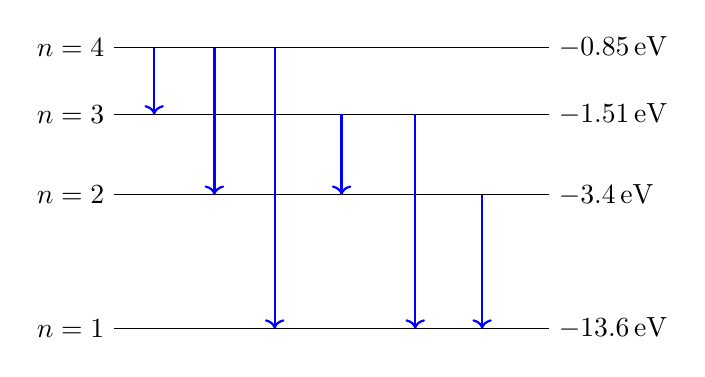
\begin{tikzpicture}[scale=.85]
\foreach \y/\n/\en in {0/1/-13.6,2/2/-3.4,3.2/3/-1.51,4.2/4/-0.85}{
\draw (0,\y)--(6.5,\y); \node[left] at (0,\y) {$n=\n$}; \node[right] at (6.5,\y) {$\en\,\mathrm{eV}$};}
\draw[->,blue,thick] (.6,4.2)--(.6,3.2);
\draw[->,blue,thick] (1.5,4.2)--(1.5,2);
\draw[->,blue,thick] (2.4,4.2)--(2.4,0);
\draw[->,blue,thick] (3.4,3.2)--(3.4,2);
\draw[->,blue,thick] (4.5,3.2)--(4.5,0);
\draw[->,blue,thick] (5.5,2)--(5.5,0);
\end{tikzpicture}
\end{center}
\crosscheck 图为定性能级图，间距非线性比例；六种为大量原子、仅考虑主量子数的可能谱线，实际跃迁还受选择定则约束。

\chapter{华中科技大学《大学物理习题册》}
\section{第1组：质点运动学}
\sourceproblem{1-T1}{1}{5}
\problemtext 平面运动 $x=3t+5,\ y=\tfrac12t^2+3t-4$（SI），求轨迹、位矢、$1$ 至 $2\,\mathrm s$ 位移、速度与加速度。
\workings 消去参数 $t=(x-5)/3$，
\[
y=\frac{(x-5)^2}{18}+x-9,\quad
\bm r=(3t+5)\bm i+(\tfrac12t^2+3t-4)\bm j.
\]
\[
\Delta\bm r=3\bm i+\tfrac92\bm j\ \mathrm m,\quad
\bm v=3\bm i+(t+3)\bm j,\quad\bm a=\bm j.
\]
速度和加速度分别采用 $\mathrm{m/s}$、$\mathrm{m/s^2}$。
\crosscheck $\bm r(1)=(8,-0.5)\,\mathrm m$，$\bm r(2)=(11,4)\,\mathrm m$；积分速度亦得相同位移。
\sourceproblem{1-T2}{1}{5}
\problemtext 初始静止于原点，$\bm a=5t^2\bm i+3\bm j$（SI）。
\workings 由两次积分并代入初值，
\[
\bm v=\tfrac53t^3\bm i+3t\bm j,\quad
\bm r=\tfrac5{12}t^4\bm i+\tfrac32t^2\bm j.
\]
运动方程即 $x=5t^4/12,\ y=3t^2/2$，轨迹为 $x=5y^2/27$（SI 数值式），$y\ge0$。
\crosscheck 对位矢连续求导两次还原题设；原点初始速度为零。
\sourceproblem{1-T3}{1}{5}
\problemtext 一维运动满足 $a=-kv^2$（$k>0$），初始 $x=0,v=v_0$，求速率关于坐标的关系。
\workings 在 $v\ne0$ 的分支上，$v\,\mathrm dv/\mathrm dx=-kv^2$，所以 $\mathrm dv/v=-k\,\mathrm dx$，得 $v=v_0e^{-kx}$，速率 $|v_0|e^{-kx}$。$v_0=0$ 时为静止解。
\crosscheck $k$ 的量纲为长度的倒数；代回得到 $v\,\mathrm dv/\mathrm dx=-kv^2$。此处是题给有向加速度，不擅自改成双向阻力模型；进一步积分得 $v(t)=v_0/(1+kv_0t)$，$x(t)=k^{-1}\ln(1+kv_0t)$，在包含初时刻的最大实解区间 $1+kv_0t>0$ 成立。对 $v_0<0$ 的正时间分支存在有限时间发散，因此不是物理上的双向阻力模型。
\sourceproblem{1-T4}{2}{6}
\problemtext 半径 $R=2\,\mathrm m$，速率 $v=KRt^2$；$v(2\,\mathrm s)=32\,\mathrm{m/s}$。求 $t=0.5\,\mathrm s$ 时速度大小和加速度大小。
\workings $K=4\,\mathrm{s^{-3}}$，故 $v=2\,\mathrm{m/s}$。
\[
a_\tau=2KRt=8\,\mathrm{m/s^2},\qquad
a_n=v^2/R=2\,\mathrm{m/s^2},
\quad a=2\sqrt{17}\,\mathrm{m/s^2}.
\]
\crosscheck 切向与法向正交；速度沿轨迹切线，题目未给绝对方位，不能指定固定坐标方向。
\sourceproblem{1-T5}{2}{6}
\problemtext 空速和正北地速均为 $135\,\mathrm{km/h}$，机头北偏东 $30^\circ$，求风速风向。
\workings 取东、北为正轴，令 $V=135\,\mathrm{km/h}$。
\[
\bm v_{\rm wind}=(-V\sin30^\circ,V(1-\cos30^\circ)).
\]
风速为 $2V\sin15^\circ\approx69.9\,\mathrm{km/h}$，风吹向西偏北 $15^\circ$，按来向命名为东偏南 $15^\circ$ 的风。
\crosscheck 风的东向分量为负，恰抵消飞机空速的东向分量；两种风向口径均已注明。

\section{第2组：质点动力学}
\sourceproblem{2-T1}{3}{7}
\problemtext 静止释放质量 $m$ 的物体，受线性阻力 $-kv$，求下落速度与终速。
\workings 取向下为正，$m\dot v=mg-kv$，$v(0)=0$。积分得 $v=mg(1-e^{-kt/m})/k$，终速 $mg/k$。
\crosscheck $k>0$；$t=0$ 时 $\dot v=g$，$k\to0$ 时 $v\to gt$。
\sourceproblem{2-T2}{3}{7}
\problemtext $m=2.00\,\mathrm{kg}$，$F=10+6x^2$（SI），从 $x=0$ 静止出发，求 $x=4.0\,\mathrm m$ 速率。
\workings 牛顿定律 $mv\,\mathrm dv/\mathrm dx=10+6x^2$；积分 $mv^2/2=10x+2x^3$，故 $v=\sqrt{168}\,\mathrm{m/s}\approx12.96\,\mathrm{m/s}$。
\crosscheck 功能关系独立核验：外力做功 $168\,\mathrm J$，等于动能增量；保留正根。
\sourceproblem{2-T3}{3}{7}
\problemtext 质量 $m$ 以 $v_0>0$ 竖直上抛，阻力与速度线性相关，求速度及最大上升高度。
\workings 向上为正，$m\dot v=-mg-kv$，解得
\[
v=(v_0+mg/k)e^{-kt/m}-mg/k.
\]
令 $v=0$ 得 $t_*=(m/k)\ln(1+kv_0/(mg))$。积分至该时刻，
\[
H=\frac{mv_0}{k}-\frac{m^2g}{k^2}\ln(1+kv_0/(mg)).
\]
\crosscheck 用 $\ln(1+z)=z-z^2/2+O(z^3)$ 检验 $k\to0$ 时 $H\to v_0^2/(2g)$；高度为相对抛出点。
\sourceproblem{2-T4}{4}{8}
\problemtext 快艇关机时速度 $v_0$，阻力大小 $kv^2$，质量 $m$，求速度、路程随时间及速度随路程的规律。
\workings 沿初速度取正，$m\dot v=-kv^2$，得
\[
v=\frac{v_0}{1+kv_0t/m},\quad
s=\frac mk\ln(1+kv_0t/m),\quad v=v_0e^{-ks/m}.
\]
\crosscheck $s(0)=0$，$\dot s=v$；速度始终为正并趋零，纯平方阻力模型下无有限停车时间。
\sourceproblem{2-T5}{4}{8}
\problemtext 水平加速度为 $a$ 的车厢内，悬挂小球相对车厢静止，求绳偏离竖直的角。
\workings 车厢系引入反向惯性力 $ma$，绳张力满足 $T\sin\theta=ma,T\cos\theta=mg$，故 $\theta=\arctan(a/g)$，绳向车加速度的反方向偏斜。
\crosscheck 地面惯性系同样有水平合力 $ma$、竖直合力零；质量约去。
\sourceproblem{2-T6}{4}{8}
\problemtext 上升加速度 $a$ 的电梯内，理想滑轮两侧悬挂 $m_1>m_2$，求张力及 $m_1$ 相对电梯的加速度。
\workings 在电梯系取有效重力 $g'=g+a$。令 $m_1$ 向下相对加速度 $b$，则 $m_1g'-T=m_1b$，$T-m_2g'=m_2b$，联立得
\[
b=\frac{m_1-m_2}{m_1+m_2}(g+a),\qquad
T=\frac{2m_1m_2}{m_1+m_2}(g+a).
\]
\crosscheck $a=0$ 退化为标准 Atwood 机，$m_1=m_2$ 时相对加速度零；假定绳绷紧。
\sourceproblem{2-T7}{5}{9}
\problemtext 教材一维冲量例题：力随时间按 $F=600-2\times10^5t$（SI）线性减小，末态速度 $300\,\mathrm{m/s}$，末态力为零；求作用时长、冲量与质量。
\workings $F(t_*)=0$ 得 $t_*=0.003\,\mathrm s$；冲量为三角形面积 $I=600t_*/2=0.9\,\mathrm{N\,s}$。在初速度为零的通常约定下，$m=I/300=0.003\,\mathrm{kg}$。
\crosscheck 若初速度未约定为零，则只能得 $m(v_f-v_i)=I$；质量数值依赖该初始条件。
\sourceproblem{2-T8}{5}{9}
\problemtext 稳定水流经直角弯管，质量流率 $3\times10^3\,\mathrm{kg/s}$、速率 $10\,\mathrm{m/s}$，求水流改变方向产生的反作用力。
\workings 入口、出口单位方向分别为 $\bm e_i,\bm e_o$，互相垂直。动量流变化率为 $\dot m v(\bm e_o-\bm e_i)$，其反向为 $\dot m v(\bm e_i-\bm e_o)$，模 $3\sqrt2\times10^4\,\mathrm N$，沿入口速度与反向出口速度的角平分线。
\crosscheck 这是忽略端面压力和流体重量的动量流反作用结果；若求真实管壁总受力，需另给端面压力、截面积与重力等条件，不能仅凭流量确定。
\sourceproblem{2-T9}{5}{9}
\problemtext 煤粉从高 $h=0.5\,\mathrm m$ 自由落至向右速率 $u=2.0\,\mathrm{m/s}$ 的带面；质量流率 $q_m=40\,\mathrm{kg/s}$，忽略已随带运动的积煤重量，求煤对带作用力。
\workings 取右和上为正，入口速度 $(0,-\sqrt{2gh})$，出口速度 $(u,0)$。忽略接触区滞留重量，带对煤的动量流作用为 $q_m(u,\sqrt{2gh})$，故煤对带力
\[
\bm F=-q_mu\,\bm i-q_m\sqrt{2gh}\,\bm j.
\]
取 $g=9.8$，得向左 $80\,\mathrm N$、向下约 $125.2\,\mathrm N$，模约 $148.6\,\mathrm N$，左下方与水平夹角 $\arctan(\sqrt{2gh}/u)\approx57.4^\circ$。
\crosscheck 水平力阻碍带运动，竖直力向下；若计入积煤或滞留煤重量，竖直负载另加。

\sourceproblem{2-T10}{6}{10}
\problemtext 均匀柔绳线密度 $\lambda$，从水平面以恒定速率 $v$ 竖直提起，求提起长度 $L$ 时拉力。
\workings 取正在上升的绳段为开系统，竖直动量 $\lambda Lv$，其增长率 $\lambda v^2$；进入绳段前竖直速度为零。故
\[
F-\lambda Lg=\lambda v^2,\qquad F=\lambda(Lg+v^2).
\]
\crosscheck 重力项随长度增加，动量通量项恒定；假定绳在提起处从静止转入竖直运动、无额外支持力作用于运动段。不可把变质量系统直接当固定质量系统。
\sourceproblem{2-T11}{6}{10}
\problemtext 卫星近地点高度439千米、远地点高度2384千米，地球半径6378千米，近地点速率8.10千米每秒，求远地点速率。
\workings 地心引力为中心力，近远地点速度垂直径矢；故
\[
v_2=v_1\frac{R+h_1}{R+h_2}
=8.10\frac{6817}{8762}\,\mathrm{km/s}\approx6.30\,\mathrm{km/s}.
\]
\crosscheck 应使用地心距离而非离地高度；远地点速率较小。
\sourceproblem{2-T12}{7}{11}
\problemtext 判断保守力正功是否增加势能、闭路保守力功、作用反作用力总功。
\workings $W_c=-\Delta U$，故正功使势能减少；闭路功为零；第三项因两物体位移可不同而不成立。仅第二项正确，选C。
\crosscheck 与天津理工第2章选择1的命题第一项措辞不同，但结论相同；两书来源编号分别保留。
\sourceproblem{2-T13}{7}{11}
\problemtext 恒力 $\bm F=4\bm i+3\bm j$（N），从原点至 $(8,6)$ 米，分别沿直线、先横后竖、先竖后横路径求功。
\workings 直线：$W=4(8)+3(6)=50\,\mathrm J$。先横后竖两段分别32和18焦耳，总50焦耳；先竖后横分别18和32焦耳，总50焦耳。任意路径的积分为 $\int(4\,\mathrm dx+3\,\mathrm dy)=4\Delta x+3\Delta y$，故为保守力，势能可取 $U=-4x-3y+C$（SI）。
\crosscheck 不仅三条指定路径相同，而且对任意可微路径成立，故保守性得到证明。
\sourceproblem{2-T14}{7}{11}
\problemtext $\bm r=a\cos\omega t\,\bm i+b\sin\omega t\,\bm j$，质量 $m$，$a>b>0$，求 $A(a,0)$、$B(0,b)$ 处动能、受力、从A到B的力及分力功，并判断保守性。
\workings $\bm v=\omega(-a\sin\omega t\,\bm i+b\cos\omega t\,\bm j)$，故 $K_A=mb^2\omega^2/2,K_B=ma^2\omega^2/2$。$\bm F=-m\omega^2(x\bm i+y\bm j)$；
\[
W_x=-m\omega^2\int_a^0 x\,\mathrm dx=\tfrac12m\omega^2a^2,\qquad
W_y=-m\omega^2\int_0^b y\,\mathrm dy=-\tfrac12m\omega^2b^2.
\]
总功 $m\omega^2(a^2-b^2)/2$。若将此力推广为整个平面上只依赖位置的上述中心力，则势能为 $m\omega^2(x^2+y^2)/2$，为保守力。
\crosscheck 总功等于动能差；仅凭单条轨迹不能唯一确定全空间力场，保守性判断明确采用位置力场模型。
\sourceproblem{2-T15}{8}{12}
\problemtext 光滑半球碗半径 $r$，质点从与向下竖直轴成 $\theta_0$ 的位置沿内面切线水平发射，求恰达水平碗口的初速。
\workings 竖直轴角动量守恒 $mr\sin\theta_0\,v_0=mr v_{\rm rim}$，临界到达碗口时沿经线速度为零。机械能守恒
\[
\tfrac12mv_0^2=\tfrac12mv_0^2\sin^2\theta_0+mgr\cos\theta_0.
\]
故 $v_0=\sqrt{2gr/\cos\theta_0}$，适用 $0\le\theta_0<\pi/2$。为验证途中可达，令 $\theta\ge\theta_0$，经线速度平方为
\[
v_\theta^2=v_0^2(1-\sin^2\theta_0/\sin^2\theta)-2gr(\cos\theta_0-\cos\theta).
\]
临界值代入后，令 $u=\cos\theta,u_0=\cos\theta_0$，对 $0<u<u_0$ 有
\[
v_\theta^2=2gr\,u\,\frac{(u_0-u)(1+u_0u)}{u_0(1-u^2)} >0.
\]
故中间没有势垒阻挡；底点情形由经线运动直接得到。
\crosscheck 光滑内面约束力不做功且对竖直轴力矩为零；碗口极限需单独处理，不能直接令 $\cos\theta_0=0$。
\sourceproblem{2-T16}{8}{12}
\problemtext 飞船在半径 $R_0$ 的圆轨道上速率为 $v_0$，变轨至近心距 $R_0$、远心距 $3R_0$ 的椭圆，求变轨后的近心点速率。
\workings 设中心天体引力参数 $\mu$，圆轨道 $v_0^2=\mu/R_0$。椭圆半长轴 $a=2R_0$，由活力公式
\[
v_p^2=\mu(2/R_0-1/(2R_0))=\tfrac32v_0^2,\qquad v_p=\sqrt{3/2}\,v_0.
\]
\crosscheck 可用近远心点角动量关系 $v_a=v_p/3$ 与机械能守恒独立推出同一结果；近心点变轨需加速。

\section{第3组：刚体定轴转动}
\sourceproblem{3-T1}{9}{13}
\problemtext 轮从静止经6秒匀加速至200转每分钟，匀速一段时间后制动，5分钟后停止，总转数3100，求总时间。
\workings 若制动为匀减速，则加速段 $N_1=100(6/60)=10$ 转，制动段 $N_3=100(5)=500$ 转，匀速段 $N_2=2590$ 转、耗时 $2590/200=12.95$ 分钟。总时间 $18.05$ 分钟，即1083秒。
\crosscheck 原题只明确加速段均匀增加，未明确制动规律；若制动非匀减速，$N_3$ 无法由端点转速和历时唯一确定，总时间也不唯一。所给数值以补充匀减速条件为前提。
\sourceproblem{3-T2}{9}{13}
\problemtext 半径1.3米圆周运动，初始 $\theta=\omega=0$，角加速度 $\beta=120t^2-48t+16$（SI），求角速度、角位置及切法向加速度。
\workings 积分得
\[
\omega=40t^3-24t^2+16t,\qquad \theta=10t^4-8t^3+8t^2.
\]
切向分量 $a_\tau=1.3(120t^2-48t+16)$，法向分量 $a_n=1.3(40t^3-24t^2+16t)^2$（SI）。
\crosscheck 两次求导恢复角加速度与初值；法向分量非负，指向圆心。
\sourceproblem{3-T3}{9}{13}
\problemtext 重物 $m$ 由静止拉动惯量 $J=MR^2/2$ 的定滑轮，求下落速度随时间的关系。
\workings $mg-T=ma,\ TR=J a/R$，故 $a=mg/(m+M/2)$，下落速率 $v(t)=mgt/(m+M/2)$。
\crosscheck 能量式 $mgh=(m+M/2)v^2/2$ 与匀加速关系一致；无滑动且轴光滑。
\sourceproblem{3-T4}{10}{14}
\problemtext 飞轮轴半径2.00厘米，20.0克物体匀速下落；改挂5.00千克物体从静止10.0秒下落40.0厘米，取 $g=9.80$，求轴摩擦力矩、惯量及第二次张力。
\workings 若摩擦力矩大小恒定，首次 $\tau_f=mg r=0.00392\,\mathrm{N\,m}$。第二次 $a=2h/t^2=0.00800\,\mathrm{m/s^2}$，$T=M(g-a)=48.96\,\mathrm N$，由 $Tr-\tau_f=J a/r$ 得
\[
J=(Tr-\tau_f)r/a=2.4382\,\mathrm{kg\,m^2}.
\]
按有效数字 $J\approx2.44\,\mathrm{kg\,m^2}$，$T\approx49.0\,\mathrm N$。
\crosscheck 两次实验须具有相同的恒定轴摩擦力矩，且绳不打滑；若摩擦随载荷或转速变化，题设不足以确定惯量。
\sourceproblem{3-T5}{10}{14}
\problemtext 两等质量 $m$、等半径 $r$ 均质滑轮与两端重物 $m,2m$ 组成系统，求两轮间张力。
\workings 取 $2m$ 端向下，整个系统等效惯性质量为 $m+2m+2(J/r^2)=4m$，故 $a=g/4$。轻端张力 $T_1=m(g+a)$，中间张力满足 $(T-T_1)r=J a/r$，得
\[
T=m(g+a)+ma/2=11mg/8.
\]
重端张力 $T_2=2m(g-a)=3mg/2$。
\crosscheck 另一滑轮满足 $T_2-T=ma/2$，与左轮一致；三段张力不可视为相等。
\sourceproblem{3-T6}{11}{15}
\problemtext 转台初始每秒1转，总惯量6.0，收臂后2.0（$\mathrm{kg\,m^2}$），求末角速率及转动动能增量。
\workings 初角速率 $\omega_i=2\pi\,\mathrm{rad/s}$。角动量守恒给出 $\omega_f=3\omega_i=6\pi\,\mathrm{rad/s}$（每秒3转）。动能差
\[
\Delta K=\tfrac12(2)(6\pi)^2-\tfrac12(6)(2\pi)^2=24\pi^2\,\mathrm J\approx237\,\mathrm J.
\]
\crosscheck $K=L_z^2/(2J)$，惯量减至三分之一使转动动能成为原来的三倍；增量来自人体做功。
\sourceproblem{3-T7}{11}{15}
\problemtext 均质细杆质量 $m$、长 $l$，端点惯量 $ml^2/3$，水平静止释放，求与向下竖直方向成30度时角速率。
\workings 质心下降 $(l/2)\cos30^\circ$，故 $mg(l/2)\cos30^\circ=(ml^2/6)\omega^2$，得 $\omega=\sqrt{3\sqrt3g/(2l)}$。
\crosscheck 初始水平时角速率零，最低点速率对应 $\omega=\sqrt{3g/l}$；本题答案介于两者之间。
\sourceproblem{3-T8}{11}{15}
\problemtext 自由旋转圆盘惯量 $J$、半径 $R$，边缘有质量 $m$ 的人，初角速率 $\omega$；人走到盘心，求角速度和动能变化。
\workings 初末惯量为 $J+mR^2,J$，故 $\omega_f=(1+mR^2/J)\omega$，
\[
\Delta\omega=mR^2\omega/J,\qquad
\Delta K=\frac{mR^2(J+mR^2)}{2J}\omega^2.
\]
\crosscheck 取人为质点，初末均相对盘静止；轴向角动量守恒，转动动能增加，不主张机械能守恒。

\sourceproblem{3-T9}{12}{16}
\problemtext 均质杆长0.4米、质量1千克，绕上端轴静止下垂；8克小物体以200米每秒水平嵌入距轴 $3l/4$ 处，求碰后角速度、最大偏角。
\workings 设 $d=3l/4$，$J=Ml^2/3+md^2$。碰撞瞬间 $\omega=mvd/J$，约 $8.88\,\mathrm{rad/s}$。随后无耗散摆动，
\[
\frac12J\omega^2=g(Ml/2+md)(1-\cos\theta_{\max}).
\]
取 $g=9.8\,\mathrm{m/s^2}$，得 $\cos\theta_{\max}\approx-0.0746$，$\theta_{\max}\approx94.3^\circ$。
\crosscheck 碰撞阶段只守恒轴向角动量，摆动阶段才守恒机械能；转动能不足以到达倒立位置。
\sourceproblem{3-T10}{12}{16}
\problemtext 长 $l$、质量 $M$ 的均质杆从与竖直成 $\theta_0$ 的位置静止下摆，在最低点与光滑地面上的静止质点 $m$ 弹性碰撞，求碰后两者速度。
\workings 端轴惯量 $J=Ml^2/3$，碰前角速率 $\omega_0=\sqrt{3g(1-\cos\theta_0)/l}$。取杆端碰前运动方向为正，碰撞满足
\[
J\omega_0=J\omega+mlv,\qquad v-l\omega=l\omega_0.
\]
解得 $\omega=(M-3m)\omega_0/(M+3m)$，$v=2Ml\omega_0/(M+3m)$。
\crosscheck 恢复系数为1；代回能量守恒。$m>M/3$ 时杆反向，不能把有向角速度强行取正。

\section{第4组：流体力学}
\sourceproblem{4-T1}{13}{17}
\problemtext 水平变截面管稳定流动，出口面积为最细处三倍，出口速率2米每秒，求最细处速度及表压，并判断细处小孔出水情形。
\workings 连续性给出 $v_1=6\,\mathrm{m/s}$。出口通大气，忽略损失，伯努利方程
\[
p_1-p_{\rm atm}=\tfrac12\rho(2^2-6^2)=-16\rho\,\mathrm{m^2/s^2}.
\]
取水密度1000千克每立方米，表压为 $-1.6\times10^4\,\mathrm{Pa}$，绝对压强为 $p_{\rm atm}-1.6\times10^4\,\mathrm{Pa}$；小孔处通常吸入空气而非向外喷水。
\crosscheck 结论以孔未开启前稳态、出口通大气且无损为前提；开启后原有流场可能改变。
\sourceproblem{4-T2}{13}{17}
\problemtext 水平管A面积10平方厘米，分支B、C面积8、6平方厘米，$v_A=1.00,v_C=0.50$（m/s），求B速度、B与C压差及最大压强所在管。
\workings $A_Av_A=A_Bv_B+A_Cv_C$，故 $v_B=0.875\,\mathrm{m/s}$。理想等高支路共享总压，
\[
p_C-p_B=\tfrac12\rho(v_B^2-v_C^2)\approx258\,\mathrm{Pa}.
\]
C速度最小，故C压强最大。
\crosscheck 假设无分支局部损失且各支路有同一上游总压；实际管网不能仅凭流速确定所有压差。
\sourceproblem{4-T3}{14}{18}
\problemtext 开口水槽液面高 $H$，孔在液面下深度 $h$，求水平射程、另一等射程孔位置、最大射程。
\workings 理想小孔流速 $\sqrt{2gh}$；孔距地 $H-h$，下落时间 $\sqrt{2(H-h)/g}$。水平射程
\[
X=2\sqrt{h(H-h)}.
\]
交换 $h$ 与 $H-h$ 射程不变，故另一孔深度 $H-h$；当 $h=H/2$ 时最大，$X_{\max}=H$。
\crosscheck $0<h<H$；两孔关于半高平面对称；水面下降及喷流阻力忽略。
\sourceproblem{4-T4}{14}{18}
\problemtext 顶部开口直立圆柱水箱，初水深0.1米，底孔面积为横截面积的1/400，求理想排空时间。
\workings 设水深 $h$，面积比 $A/a=400$，连续性及托里拆利公式给出 $A\dot h=-a\sqrt{2gh}$，积分
\[
t=\frac{A}{a}\sqrt{\frac{2h_0}{g}}
=400\sqrt{\frac{0.2}{g}}\approx57.1\,\mathrm s
\]
（$g=9.8$）。若保留自由液面速度，乘以 $\sqrt{1-(a/A)^2}$，变化极小。
\crosscheck 液面高度变化不可用初始出流速度直接除以体积；真实排水需考虑流量系数。

\section{第5组：狭义相对论}
\sourceproblem{5-T1}{17}{21}
\problemtext 不稳定粒子的固有寿命为 $\tau_0$，实验室速度为 $u$，求平均寿命对应的飞行距离。扫描页寿命指数较模糊，本条以符号形式保留。
\workings 实验室寿命 $\tau=\gamma\tau_0$，$\gamma=(1-u^2/c^2)^{-1/2}$，故
\[
L=u\gamma\tau_0.
\]
若原页速度读作 $2\times10^8\,\mathrm{m/s}$，取 $c=3\times10^8\,\mathrm{m/s}$，则 $L=(6/\sqrt5)\times10^8\tau_0$（SI）。
\crosscheck 固有时间为粒子自身时钟的时间；原图寿命指数待高分辨率二校，暂不填写未经确认的数值答案。本条标为条件式待核。
\sourceproblem{5-T2}{17}{21}
\problemtext 静止正方形面积100平方米，观察系沿其一条对角线以 $0.8c$ 运动，求观察系同时测量的面积。
\workings 沿运动方向尺寸缩短为 $\sqrt{1-0.8^2}=0.6$ 倍，垂直方向不变；平面面积的线性变换行列式为0.6，故面积为 $60\,\mathrm{m^2}$。
\crosscheck 形状一般变为菱形；不能将两条边均直接乘0.6，也不是照片的视觉面积。
\sourceproblem{5-T3}{18}{22}
\problemtext 刚性尺静止于 $S'$，与 $x'$ 轴成30度；在沿正 $x$ 轴相对运动的 $S$ 中测得与 $x$ 轴成45度，求相对速度。
\workings 同时测量有 $L_x=L'_x/\gamma,L_y=L'_y$，故 $\tan45^\circ=\gamma\tan30^\circ$，$\gamma=\sqrt3$。因此 $u=c\sqrt{2/3}\approx0.816c$。
\crosscheck 运动方向长度收缩使倾角增大；测量两端须在 $S$ 中同时进行。
\sourceproblem{5-T4}{18}{22}
\problemtext 两飞船固有长度各100米；甲船测量自身前端通过乙船全长的时间 $\Delta t$，求相对速率。扫描时标读作 $(8/3)\times10^{-7}\,\mathrm s$，指数保留二校标记。
\workings 甲系内乙船长度为 $L_0/\gamma$，故 $\Delta t=L_0/(\gamma u)$。解得
\[
u=\frac{c}{\sqrt{1+(c\Delta t/L_0)^2}}.
\]
按上述时标，$c\Delta t/L_0=0.8$，故 $u=5c/\sqrt{41}\approx0.781c$。
\crosscheck 两通过事件发生在甲船前端同一位置；不应把甲船全长也加进通过距离。若时标指数复核改变，使用保留的通式重算。
\sourceproblem{5-T5}{19}{23}
\problemtext 粒子在 $S'$ 中速率 $c/2$、与 $x'$ 轴夹60度，初始通过公共原点；$S'$ 沿 $S$ 正 $x$ 轴以 $0.6c$ 运动，求 $S$ 中运动方程。
\workings $u'_x=c/4,u'_y=\sqrt3c/4$，相对论速度变换给出
\[
u_x=\frac{u'_x+0.6c}{1+0.6u'_x/c}=\frac{17c}{23},\qquad
u_y=\frac{u'_y\sqrt{1-0.6^2}}{1+0.6u'_x/c}=\frac{4\sqrt3c}{23}.
\]
故 $x=17ct/23,\ y=4\sqrt3ct/23$。
\crosscheck 合速率 $c\sqrt{337}/23<c$，并可由洛伦兹坐标变换消去 $t'$ 验证。
\sourceproblem{5-T6}{19}{23}
\problemtext 列车速度 $0.6c$，车上A、B沿车轴相距10米且B在前；地面系记录A处事件后12.5纳秒发生B处事件。求车内系事件先后。
\workings 地面同时测得车内间距 $10/\gamma=8\,\mathrm m$，两事件空间差 $\Delta x=8+0.6c\Delta t=10.25\,\mathrm m$。洛伦兹变换
\[
\Delta t'=\gamma(\Delta t-0.6\Delta x/c)=-10\,\mathrm{ns}.
\]
车内系中B处事件早于A处事件10纳秒。
\crosscheck $c\Delta t=3.75\,\mathrm m<\Delta x$，两事件为空间样间隔，先后可随参考系改变；不能把事件先后等同于因果关系。

\sourceproblem{5-T7}{20}{24}
\problemtext 实验室中两个电子沿相反方向以相同速率 $0.67c$ 运动，求相对速率。
\workings 共线速度变换给出 $u_{\rm rel}=2(0.67)c/(1+0.67^2)\approx0.925c$。
\crosscheck 结果小于光速；不能用经典速度相加得到 $1.34c$。
\sourceproblem{5-T8}{20}{24}
\problemtext 原子核以 $0.5c$ 远离观察者，沿运动方向发射相对核速率 $0.8c$ 的电子，又向观察者方向发射光子，求观察者测得两者速率。
\workings 远离方向为正，$u_e=(0.8+0.5)c/(1+0.8\cdot0.5)=13c/14$。光子在核系速度为 $-c$，变换后 $u_\gamma=(-1+0.5)c/(1-0.5)=-c$，速率为 $c$。
\crosscheck 电子速率小于光速，光子速率在惯性系间不变。
\sourceproblem{5-T9}{21}{25}
\problemtext S系光子沿与正 $x$ 轴成60度方向传播，S'沿正 $x$ 以 $0.6c$ 运动，求S'中的方向及速率。
\workings
\[
u'_x=\frac{c/2-0.6c}{1-0.6/2}=-c/7,\quad
u'_y=\frac{(\sqrt3c/2)\sqrt{1-0.6^2}}{1-0.6/2}=4\sqrt3c/7.
\]
所以 $\theta'=\arccos(-1/7)\approx98.21^\circ$，速率为 $c$。
\crosscheck 两分量平方和为 $c^2$；方向在第二象限，不能直接取反正切主值。
\sourceproblem{5-T10}{21}{25}
\problemtext 质量 $m_0$ 的粒子分别从静止加速至 $0.100c$、从 $0.900c$ 加速至 $0.980c$，求外力净功。
\workings 相对论动能 $K=(\gamma-1)m_0c^2$，故
\[
W_1=(1/\sqrt{0.99}-1)m_0c^2\approx0.005038m_0c^2,
\quad W_2=(1/\sqrt{1-0.98^2}-1/\sqrt{1-0.90^2})m_0c^2
\approx2.7307m_0c^2.
\]
\crosscheck 两功均为正；高速区不能使用经典动能差。题面未给静质量数值，因此以 $m_0c^2$ 表示。
\sourceproblem{5-T11}{22}{26}
\problemtext 电子动能1 MeV、静能0.511 MeV，求动量大小。
\workings $E=K+m_0c^2=1.511\,\mathrm{MeV}$，由 $E^2=p^2c^2+m_0^2c^4$ 得
\[
p=\sqrt{1.511^2-0.511^2}\,\mathrm{MeV}/c
=\sqrt{2.022}\,\mathrm{MeV}/c\approx1.422\,\mathrm{MeV}/c.
\]
换算约 $7.60\times10^{-22}\,\mathrm{kg\,m/s}$。
\crosscheck $pc=\sqrt{K(K+2m_0c^2)}$，不能把动能误当总能量。
\sourceproblem{5-T12}{22}{26}
\problemtext 静止质量42u的粒子衰变为两碎片，其中一片静质量20u、速率 $3c/5$，求另一片动量、总能量和静质量。
\workings 第一片 $\gamma=5/4$，$E_1=25\,\mathrm u c^2$、$p_1=15\,\mathrm u c$。由四动量守恒，第二片 $\bm p_2=-\bm p_1$，$E_2=(42-25)\,\mathrm u c^2=17\,\mathrm u c^2$，
\[
m_2=\sqrt{17^2-15^2}\,\mathrm u=8\,\mathrm u .
\]
按题给 $1\,\mathrm u=1.66\times10^{-27}\,\mathrm{kg}$、$c=3\times10^8\,\mathrm{m/s}$，$p_2=7.47\times10^{-18}\,\mathrm{kg\,m/s}$，$E_2\approx2.54\times10^{-9}\,\mathrm J$，$m_2=1.328\times10^{-26}\,\mathrm{kg}$。
\crosscheck 第二片速率 $p_2c^2/E_2=15c/17<c$，两片动量相反，总能量等于母粒子静能。

\section{第6组：静电场}
\sourceproblem{6-T1}{23}{27}
\problemtext 半径 $R$ 的细带电圆环，线电荷密度随从正 $x$ 轴量起的极角变化为 $\lambda=\lambda_0\sin\theta$，求环心场强。
\workings $\mathrm dq=\lambda_0R\sin\theta\,\mathrm d\theta$，环心的场元为
\[
\mathrm d\bm E=-\frac{\lambda_0}{4\pi\varepsilon_0R}\sin\theta(\cos\theta\bm i+\sin\theta\bm j)\,\mathrm d\theta.
\]
在 $0$ 到 $2\pi$ 积分，交叉项为零，$\int\sin^2\theta\,\mathrm d\theta=\pi$，故 $\bm E=-\lambda_0\bm j/(4\varepsilon_0R)$。
\crosscheck 若 $\lambda_0>0$，上半环正电、下半环负电，对环心场均向下；净电荷为零不代表场为零。
\sourceproblem{6-T2}{23}{27}
\problemtext 无限均匀带电平面面密度 $\sigma$，距平面 $z>0$ 的P点，证明半径 $\sqrt3 z$ 的同轴圆盘区域贡献一半场强。
\workings 半径 $s$ 的环元电荷 $2\pi\sigma s\,\mathrm ds$，轴向场为
\[
E_z(a)=\frac{\sigma z}{2\varepsilon_0}\int_0^a\frac{s\,\mathrm ds}{(s^2+z^2)^{3/2}}
=\frac{\sigma}{2\varepsilon_0}\left(1-\frac{z}{\sqrt{z^2+a^2}}\right).
\]
当 $a=\sqrt3z$ 时括号等于 $1/2$，故圆盘贡献为无限平面场 $\sigma/(2\varepsilon_0)$ 的一半。
\crosscheck $a\to\infty$ 恢复无限平面结果；$a\to0$ 时场趋零。
\sourceproblem{6-T3}{24}{28}
\problemtext 半径 $R$ 的均匀带电半球曲面面密度 $\sigma$，求球心场强。
\workings 令 $\theta$ 为从半球向内对称轴（指向带电半球）量起的角，环元面积 $2\pi R^2\sin\theta\,\mathrm d\theta$。在球心，轴向场沿反向，
\[
E_{\parallel}=-\frac{\sigma}{2\varepsilon_0}\int_0^{\pi/2}\cos\theta\sin\theta\,\mathrm d\theta
=-\frac{\sigma}{4\varepsilon_0}.
\]
依原图，带电半球位于左方，若 $\sigma>0$，场指向右方开口，大小 $|\sigma|/(4\varepsilon_0)$。
\crosscheck 横向分量由轴对称抵消；两相反半球均匀同密度合成完整球面时中心场相消。
\sourceproblem{6-T4}{24}{28}
\problemtext 厚度 $d$ 的非导体无限平板，均匀体电荷密度 $\rho$，求板内外场强。
\workings 取中面为 $z=0$，垂直板面的正向为 $\bm e_z$，用对称薄盒高斯面得
\[
\bm E(z)=\begin{cases}
\rho z\,\bm e_z/\varepsilon_0,& |z|\le d/2,\\
\rho d\,\mathrm{sgn}(z)\bm e_z/(2\varepsilon_0),& |z|>d/2.
\end{cases}
\]
\crosscheck 两表面场连续，因为没有附加面电荷；中面场为零。原书未给横向尺寸，采用无限平板模型，有限板需考虑边缘效应。
\sourceproblem{6-T5}{25}{29}
\problemtext 点电荷 $q$ 位于正方体中心或一个顶点时，分别求每面电通量。
\workings 中心情形由六面等价及高斯定理，每面为 $q/(6\varepsilon_0)$。顶点情形，将八个同样正方体拼成大立方体使电荷居中心；每个大外面通量 $q/(6\varepsilon_0)$，分为四个等价小面，故原立方体不经过电荷的三个外面各为 $q/(24\varepsilon_0)$。经过该顶点的三个面除奇点外场平行于面，通量按去除奇点的积分为零。
\crosscheck 三个外面之和为 $q/(8\varepsilon_0)$；电荷位于边界，不能未经说明直接套用闭合面内部点电荷公式。
\sourceproblem{6-T6}{25}{29}
\problemtext 半径 $R$ 的球内 $\rho(r)=\rho_0(1-r/R)$，求内外场及最大场强位置。
\workings 球对称积分 $Q(r)=4\pi\rho_0(r^3/3-r^4/(4R))$（$r\le R$），总电荷 $Q(R)=\pi\rho_0R^3/3$，因此
\[
E_r=\begin{cases}
\frac{\rho_0}{\varepsilon_0}(r/3-r^2/(4R)),&0\le r\le R,\\
\frac{\rho_0 R^3}{12\varepsilon_0r^2},&r>R .
\end{cases}
\]
对内区大小求极值，$1/3-r/(2R)=0$ 给出 $r=2R/3$，$E_{\max}=|\rho_0|R/(9\varepsilon_0)$（$\rho_0\ne0$）。
\crosscheck 边界两式均给 $\rho_0R/(12\varepsilon_0)$，小于峰值；外区随 $r$ 单调减小，故为全局最大。
\sourceproblem{6-T7}{26}{30}
\problemtext 无限长均匀带电实心圆柱半径 $R$、体密度 $\rho$，证明内场并求外场。
\workings 取半径 $r$、长度 $L$ 的同轴高斯圆柱，端面通量为零。由 $2\pi rLE_r=\rho\pi L\min(r^2,R^2)/\varepsilon_0$ 得
\[
E_r=\begin{cases}
\rho r/(2\varepsilon_0),&0\le r\le R,\\
\rho R^2/(2\varepsilon_0r),&r>R .
\end{cases}
\]
\crosscheck 在 $R$ 处连续；外部相当于线密度 $\lambda=\pi R^2\rho$ 的无限线电荷。
\sourceproblem{6-T8}{26}{30}
\problemtext 同心球壳区域 $a<r<b$ 内体密度 $\rho=A/r$，空腔中心有点电荷 $Q$，求使带电区域场强大小恒定的 $A$。
\workings 对 $a<r<b$，包围净电荷为 $Q+4\pi A\int_a^r s\,\mathrm ds=Q+2\pi A(r^2-a^2)$。因此
\[
E_r=\frac{A}{2\varepsilon_0}+\frac{Q-2\pi Aa^2}{4\pi\varepsilon_0r^2}.
\]
要使连续区间内场强大小恒定，第二项系数必须为零，故 $A=Q/(2\pi a^2)$，恒定大小 $|Q|/(4\pi\varepsilon_0a^2)$。
\crosscheck 场强有向分量连续；非零恒定大小意味着该连通区间内方向符号不变，故消去 $r^{-2}$ 项是必要且充分的。量纲 $A$ 为电荷/面积。

\section{第7组：恒定磁场}
\sourceproblem{7-T1}{36}{40}
\problemtext 原点处电流元 $I\mathrm dl$ 沿正 $y$，求六个指定坐标点的磁场贡献。
\workings 设 $a>0$、$K=\mu_0 I\mathrm dl/(4\pi a^2)$。毕奥--萨伐尔定律给出
\[
\mathrm d\bm B=\frac{\mu_0 I\mathrm dl}{4\pi}\frac{z\bm i-x\bm k}{(x^2+y^2+z^2)^{3/2}}.
\]
对原书依次给出的 $(a,0,0),(0,a,0),(0,0,a),(a,a,0),(0,-a,a),(a,a,a)$，结果依次为
\[
-K\bm k,\quad 0,\quad K\bm i,\quad
-\frac{K}{2\sqrt2}\bm k,\quad
\frac{K}{2\sqrt2}\bm i,\quad
\frac{K}{3\sqrt3}(\bm i-\bm k).
\]
\crosscheck 所求仅为原点电流元的贡献，不能将其误作整根长直导线的场；与电流元共线的点叉积为零。
\sourceproblem{7-T2}{36}{40}
\problemtext 两同心圆弧半径 $a>b$、张角 $\theta$，两端以径向直线连接成载流闭路，求圆心P的磁场。
\workings 径向段贡献为零；图示外弧顺时针、内弧逆时针，故取纸面向外为正，
\[
\bm B_P=\frac{\mu_0I\theta}{4\pi}(1/b-1/a)\bm e_z.
\]
\crosscheck $\theta$ 必须采用弧度；两弧场相减，内弧因半径较小而占优。
\sourceproblem{7-T3}{37}{41}
\problemtext 无限长导线中央一段弯为半径 $a$、圆心角120度的上方圆弧，两侧水平半无限直段相连，电流向右，求圆心P场强。
\workings 弧段 $B_{\rm arc}=\mu_0 I(2\pi/3)/(4\pi a)=\mu_0 I/(6a)$。直段与P垂距为 $a/2$，各段近端沿水平的距离为 $\sqrt3a/2$，故各段场为 $\mu_0 I(1-\sqrt3/2)/(2\pi a)$。三段方向均入纸面，因此
\[
B=\frac{\mu_0 I}{a}\left[\frac16+\frac{1-\sqrt3/2}{\pi}\right].
\]
\crosscheck 直段积分范围不包含垂足；圆弧及直段用右手定则所得方向一致。
\sourceproblem{7-T4}{37}{41}
\problemtext 半径 $R$ 的绝缘圆盘均匀带电 $q$，以角速度 $\omega$ 绕中心法线旋转，证明盘心磁场与磁偶极矩。
\workings 面密度 $q/(\pi R^2)$，半径 $r$、宽 $\mathrm dr$ 的环带电荷 $\mathrm dq=2qr\,\mathrm dr/R^2$，电流 $\mathrm dI=\omega\,\mathrm dq/(2\pi)$。故
\[
B=\int_0^R \frac{\mu_0\mathrm dI}{2r}=\frac{\mu_0\omega q}{2\pi R},\qquad
p_m=\int_0^R\pi r^2\mathrm dI=\frac{\omega qR^2}{4}.
\]
这里按正电荷和角速率记大小；矢量方向沿 $q\bm\omega$。
\crosscheck 两式均与原书目标一致；积分在 $r=0$ 处有限，不需要额外内孔。
\sourceproblem{7-T5}{38}{42}
\problemtext 两半径 $R$ 的同向载流圆环共轴，圆心距 $a$，求轴线任意点磁场并证明 $a=R$ 时中点附近最均匀。
\workings 取中点为原点，令 $f(s)=(R^2+s^2)^{-3/2}$，则轴向磁场大小
\[
B(x)=\frac{\mu_0IR^2}{2}[f(x-a/2)+f(x+a/2)].
\]
偶对称使 $B'(0)=0$。而 $f''(s)=3(4s^2-R^2)/(R^2+s^2)^{7/2}$，故
\[
B''(0)=\frac{3\mu_0IR^2(a^2-R^2)}{(R^2+a^2/4)^{7/2}}.
\]
唯一正间距 $a=R$ 消去二阶项；奇阶项亦因对称性消失，中点附近首个变化为四阶量。此时 $B(0)=(4/5)^{3/2}\mu_0I/R$。
\crosscheck “最均匀”指中点附近的局部轴向泰勒展开，并非整个空间磁场恒定。
\sourceproblem{7-T6}{38}{42}
\problemtext 图示三棱柱处于沿正 $x$ 轴的2.0特斯拉匀强场中，求三个矩形侧面 $abcd,befc,aefd$ 的磁通量。
\workings 采用闭合棱柱外法向，面 $abcd$ 位于 $yz$ 平面，面积 $0.40\times0.30$ 平方米，外法向负 $x$，故 $\Phi_{abcd}=-0.24\,\mathrm{Wb}$。面 $befc$ 位于 $xy$ 平面，磁场平行于面，故 $\Phi_{befc}=0$。上下三角面也与磁场平行；由闭合磁通为零，$\Phi_{aefd}=+0.24\,\mathrm{Wb}$。
\crosscheck 斜面沿 $yz$ 平面的正投影面积同为0.12平方米，可独立核验；若题目只要求大小，分别为0.24、0、0.24韦伯。

\section{第8组：电磁感应}
\sourceproblem{8-T1}{44}{48}
\problemtext 长直导线与矩形框共面，框平行边长 $l$、宽 $b$，初始近边距 $a$。分别讨论恒电流时框远离、交变电流时框静止、交变电流时框远离的电动势。
\workings 取正法向为直线正电流在框处的磁场方向，近边距 $s=a+vt$ 时
\[
\Phi=\frac{\mu_0 l I(t)}{2\pi}\ln\frac{s+b}{s},\qquad
\mathcal E=\frac{\mu_0 l}{2\pi}\left[\frac{I(t)vb}{s(s+b)}-\dot I(t)\ln\frac{s+b}{s}\right].
\]
第一问 $\dot I=0$；第二问 $v=0,s=a,I=I_m\sin\omega t$；第三问两项同时保留，$\dot I=I_m\omega\cos\omega t$。
\crosscheck 总磁通导数同时包括运动与磁场变化，不能只保留其中一项；正负由选定回路方向决定。
\sourceproblem{8-T2}{44}{48}
\problemtext 矩形框在 $Oxz$ 平面中以速率 $v$ 沿正 $x$ 方向移动，磁场沿 $y$ 方向，$B=B_0\cos[\omega(t-x/c)]$；框横向边长 $l_1$、沿运动方向边长 $l_2$，初始ab边与 $z$ 轴重合。
\workings 取正 $y$ 为法向，令 $k=\omega/c,\Omega=\omega-kv$，则
\[
\Phi=B_0l_1\int_{vt}^{vt+l_2}\cos(\omega t-kx)\,\mathrm dx
=\frac{2B_0l_1}{k}\sin(kl_2/2)\cos(\Omega t-kl_2/2).
\]
故 $\mathcal E=2B_0l_1(\Omega/k)\sin(kl_2/2)\sin(\Omega t-kl_2/2)$。
\crosscheck $v=c$ 时磁通不变；高清PDF48确认传播相位坐标及运动方向均为 $x$，ab边长 $l_1$，ad边长 $l_2$。通式由实际运动方向上的场分布决定。
\sourceproblem{8-T3}{45}{49}
\problemtext 5厘米乘10厘米矩形框以2厘米每秒进入宽20厘米的垂直均匀磁场区域，$B=0.1$ T，求磁通和电动势随时间变化。
\workings 按图运动方向边长 $a=0.10$ m，垂直边长 $h=0.05$ m，场区宽 $D=0.20$ m；首次接触时 $t=0$。取磁场方向为正，
\[
\Phi(t)=Bh\begin{cases}vt,&0\le t<5,\\a,&5\le t<10,\\D+a-vt,&10\le t<15,\\0,&t\ge15.\end{cases}
\]
相应电动势为 $-10^{-4}$ V、0、$+10^{-4}$ V、0；进入和离开方向相反，磁通平台为 $5\times10^{-4}$ Wb。
\crosscheck 原图长边平行运动方向；若取顺时针正向且场入纸面，则上述符号一致。理想尖锐边界的折点导数不定义。
\sourceproblem{8-T4}{45}{49}
\problemtext 夹角 $\theta$ 的金属架与竖直滑杆MN组成三角回路，杆自顶点以恒速 $v$ 向右，磁场垂直纸面向外。求均匀恒定场及 $B=Kx\cos\omega t$ 时电动势。
\workings 取逆时针为正，$X=vt$，截面高度 $x\tan\theta$。恒场时 $\Phi=B X^2\tan\theta/2$，$\mathcal E=-Bv^2t\tan\theta$。非均匀场时
\[
\Phi=\frac{KX^3}{3}\tan\theta\cos\omega t,\quad
\mathcal E=-Kv^3\tan\theta[t^2\cos\omega t-\omega t^3\sin\omega t/3].
\]
\crosscheck 第二问包含移动边界与显式时间变化两项；负值对应顺时针方向。
\sourceproblem{8-T5}{46}{50}
\problemtext 水平金属圆环半径10厘米、电阻1欧，地磁场竖直分量为 $5\times10^{-5}$ T，翻转一次，求通过截面的电荷量。
\workings 忽略初末自感电流，积分电路方程得 $|q|=|\Delta\Phi|/R=2B_z\pi r^2/R$，按上述读数为 $3.14\times10^{-6}$ C。
\crosscheck 180度翻转磁通变号，与翻转快慢无关；高清PDF50确认指数为负5。
\sourceproblem{8-T6}{46}{50}
\problemtext 平均半径12厘米、$N=4\times10^3$ 匝的线圈在0.5 G地磁场中每秒转30圈，求最大感应电动势及取得条件。
\workings $B=5\times10^{-5}$ T，$\omega=60\pi$ rad/s，若转轴垂直于磁场，则
\[
\mathcal E_m=NB\pi(0.12)^2(60\pi)\approx4.264\times10^{-4}N\,\mathrm V .
\]
框面与磁场平行时取最大绝对值；若轴与场夹角为 $\beta$，有效场为 $B|\sin\beta|$。
\crosscheck 高清PDF50确认匝数为4000，故最大电动势约为 $1.71\,\mathrm V$。
\sourceproblem{8-T7}{46}{50}
\problemtext 两水平平行导轨间距 $l$，一端接电阻 $R$，质量 $m$ 的金属棒以初速度 $v_0$ 向左，垂直均匀磁场 $B$ 中无摩擦滑动，求速度、位移及能量关系。
\workings 忽略自感及其他电阻，$i=Blv/R$，磁力反向且大小 $B^2l^2v/R$。取向左为位移正向，令 $\tau=mR/(B^2l^2)$，
\[
v=v_0e^{-t/\tau},\quad x=v_0\tau(1-e^{-t/\tau}).
\]
电阻热 $Q=\int_0^t i^2R\,\mathrm dt=mv_0^2(1-e^{-2t/\tau})/2$，恰等于动能减少。
\crosscheck 有限时刻速度仍为正；极限位移为 $v_0\tau$。机械能转化为焦耳热，含热的总能量守恒。
\sourceproblem{8-T8}{47}{51}
\problemtext 长 $L$ 的导线绕固定端O在长直载流导线所在平面内旋转，O距直线 $a>L$，求杆与向右水平成 $\theta$ 时的动生电动势。
\workings 取直线电流向上、逆时针角速度 $\omega$ 为正，杆上距O为 $s$ 的点距直线 $a+s\cos\theta$，磁场入纸面。故从O至杆端
\[
\mathcal E=-\frac{\mu_0 I\omega}{2\pi}\int_0^L\frac{s\,\mathrm ds}{a+s\cos\theta}
=-\frac{\mu_0 I\omega}{2\pi\cos^2\theta}
\left[L\cos\theta-a\ln(1+L\cos\theta/a)\right].
\]
当 $\cos\theta=0$ 时取极限 $-\mu_0 I\omega L^2/(4\pi a)$。若按图实际顺时针旋转，则有向 $\omega<0$。
\crosscheck $a>L$ 保证杆不穿过直线奇点；远场恢复均匀场旋转杆公式。
\sourceproblem{8-T9}{47}{51}
\problemtext 两圆形磁场区域半径21.2、32.3厘米，初始场强大小48.6、77.2毫特斯拉，左区入纸面、右区出纸面，两场大小均以 $8.5\,\mathrm{mT/s}$ 减小，求原图三个有向回路的感生电场环流。
\workings 高清PDF51确认a逆时针、b顺时针、c逆时针。取纸外为正，令 $k=0.0085\,\mathrm{T/s}$，则左区 $\dot B_1=+k$、右区 $\dot B_2=-k$。按原图各回路的定向，
\[
\oint_a\bm E\cdot\mathrm d\bm l=-k\pi R_1^2\approx-1.20\,\mathrm{mV},\quad
\oint_b\bm E\cdot\mathrm d\bm l=-k\pi R_2^2\approx-2.79\,\mathrm{mV},
\]
\[
\oint_c\bm E\cdot\mathrm d\bm l=k\pi(R_2^2-R_1^2)\approx1.59\,\mathrm{mV}.
\]
\crosscheck c回路对左右区使用同一纸外法向，而b回路使用纸内法向，故不能直接将a、b的环流相加；初始场强不进入磁通变化率。

\section{第9组：气体分子运动论}
\sourceproblem{9-T1}{55}{59}
\problemtext 氧气瓶容积 $3.2\times10^{-2}$ 立方米，初压 $1.30\times10^7$ Pa，补气阈值 $1.0\times10^6$ Pa，每日耗用常压 $1.01\times10^5$ Pa 下0.40立方米氧气，等温求可用天数。
\workings 由 $pV=Nk_BT$，可消耗分子数为 $(p_i-p_f)V/(k_BT)$，每日用量为 $p_dV_d/(k_BT)$。故
\[
t=\frac{(1.30\times10^7-1.0\times10^6)0.032}{1.01\times10^5(0.40)}\approx9.50\ \text{天}.
\]
\crosscheck 不可将瓶内剩余气体全部计为可用；高压氧气的非理想性按教材理想模型忽略。
\sourceproblem{9-T2}{55}{59}
\problemtext 真空压强 $1.01325\times10^{-10}$ Pa、温度25摄氏度，求数密度，并与标准状况比较。
\workings $n=p/(k_BT)$，取 $k_B=1.380649\times10^{-23}$ J/K，$T=298.15$ K，得 $n\approx2.46\times10^{10}\,\mathrm{m^{-3}}$。标准状况取101325 Pa和273.15 K，$n_0\approx2.69\times10^{25}\,\mathrm{m^{-3}}$，约为前者的 $1.09\times10^{15}$ 倍。
\crosscheck 已放大原页确认真空压强指数负10；真空并非完全没有分子。
\sourceproblem{9-T3}{56}{60}
\problemtext 解释原题八个关于速率分布函数的式子。
\workings 设总分子数 $N$、速率分布密度 $f(v)$、区间 $A=[v_1,v_2]$，单分子质量 $m$。依原书顺序：(1) $f(v)=\mathrm dN/(N\mathrm dv)$ 为速率概率密度；(2) $f(v)\mathrm dv$ 为微小速率区间的分子比例；(3) $Nf(v)\mathrm dv$ 为该区间分子数；(4) $\int_A f(v)\mathrm dv$ 为有限区间比例；(5) $N\int_A f(v)\mathrm dv$ 为该区间分子数；(6) $\int_A vf(v)\mathrm dv/\int_A f(v)\mathrm dv$ 为区间条件平均速率；(7) $N\int_A mv^2f(v)\mathrm dv/2$ 为区间分子平动动能总和；(8) $\int_A mv^2f(v)\mathrm dv/[2\int_A f(v)\mathrm dv]$ 为该区间每分子平均平动动能。
\crosscheck 条件平均的分母必须非零；$f$ 的量纲为速率的倒数，不能把概率密度本身当概率。
\sourceproblem{9-T4}{56}{60}
\problemtext 同温氢气和氧气的麦克斯韦速率分布，右峰最概然速率2000 m/s，求两气体最概然速率及温度。
\workings $v_p=\sqrt{2RT/M}$，较轻的氢气对应右峰II，氧气对应I。摩尔质量比16，故 $v_{p,\mathrm O_2}=500$ m/s。取氢气摩尔质量 $0.002$ kg/mol，$T=Mv_p^2/(2R)\approx481$ K。
\crosscheck 图中横坐标2000已核实；不由示意图左峰位置直接估读，使用质量平方根关系。
\sourceproblem{9-T5}{57}{61}
\problemtext 气体方均根速率450 m/s、压强 $7\times10^4$ Pa，求质量密度。
\workings 气体动理论 $p=\rho\overline{v^2}/3$，故 $\rho=3p/(450)^2\approx1.037\,\mathrm{kg/m^3}$。
\crosscheck 方均根速率的平方才是均方速率。
\sourceproblem{9-T6}{57}{61}
\problemtext 氧气压强 $1.01\times10^5$ Pa、温度27摄氏度，求分子数密度、质量密度、分子平均平动动能。
\workings $T=300.15$ K，$n=p/(k_BT)\approx2.44\times10^{25}\,\mathrm{m^{-3}}$；取 $M=0.032$ kg/mol，$\rho=pM/(RT)\approx1.30\,\mathrm{kg/m^3}$；$\overline K=3k_BT/2\approx6.22\times10^{-21}$ J。
\crosscheck 平动能只含三个平动自由度，不使用双原子总能量的5/2系数。
\sourceproblem{9-T7}{57}{61}
\problemtext 容积 $1.0\times10^{-3}$ 立方米内有 $1.01\times10^{23}$ 个氢气分子，压强 $1.01\times10^5$ Pa，求温度和方均根速率。
\workings $T=pV/(Nk_B)\approx72.43$ K，$v_{\rm rms}=\sqrt{3RT/M}\approx950$ m/s（$M=0.002$ kg/mol）。
\crosscheck 原页三个指数已高清核实；可直接由 $v_{\rm rms}^2=3pV/(Nm)$ 独立验证。
\sourceproblem{9-T8}{58}{62}
\problemtext 刚性双原子理想气体体积 $2.0\times10^{-3}$ 立方米、内能675 J，分子数 $5.4\times10^{22}$，求压强、平均平动动能和温度。
\workings 刚性双原子 $U=5Nk_BT/2=5pV/2$，故 $p=1.35\times10^5$ Pa；每分子平均平动能 $3U/(5N)=7.50\times10^{-21}$ J，$T=2U/(5Nk_B)\approx362$ K。
\crosscheck 按题给刚性模型忽略振动；内能与平动能不是同一概念。
\sourceproblem{9-T9}{58}{62}
\problemtext 1 mol双原子气体在27摄氏度，求全体分子的平动与转动动能总和。
\workings 刚性双原子分子有三个平动、两个转动自由度。$E_{\rm tr}=3RT/2\approx3.74\times10^3$ J，$E_{\rm rot}=RT\approx2.50\times10^3$ J。
\crosscheck 原题问1 mol的总贡献，不是每分子能量；若求每分子则将 $R$ 改为 $k_B$。
\sourceproblem{9-T10}{58}{62}
\problemtext 1 mol水蒸气分解为同温1 mol氢气和半mol氧气，不计振动自由度，求内能增长百分比。
\workings 非线性水分子有6个平动转动自由度，热运动内能 $U_i=3RT$。产物为1.5 mol刚性双原子气体，$U_f=1.5(5RT/2)=15RT/4$，故 $(U_f-U_i)/U_i=25\%$。
\crosscheck 25\%仅为教材自由度模型的热运动内能变化；实际化学分解涉及键能和化学内能，不能用该百分比代替反应内能。

\sourceproblem{9-T11}{59}{63}
\problemtext 刚性分子自由度 $i=t+r$，气体质量 $m$、摩尔质量 $M$，解释原题六个能量表达式。
\workings 按原序：(1) $k_BT/2$ 是单个二次型自由度的平均能量；(2) $3k_BT/2$ 是每分子平均平动动能；(3) $ik_BT/2$ 是每分子平均平动及转动动能；(4) $iRT/2$ 是每摩尔热运动内能；(5) $(m/M)3RT/2$ 是全体分子平动动能；(6) $(m/M)iRT/2$ 是该气体热运动内能。
\crosscheck 采用经典能量均分、理想气体及无振动的刚性模型；$m/M$ 的量纲为摩尔。
\sourceproblem{9-T12}{59}{63}
\problemtext $N$ 个质量均为 $m$ 的分子，图示数密度函数 $Nf(v)$ 从0到 $v_0$ 线性升至 $a$，再至 $2v_0$ 保持 $a$，其余为零。求面积意义、$a$、区间 $[v_0/2,3v_0/2]$ 内分子数及平均平动动能。
\workings 图下面积为总分子数，$N=av_0/2+av_0=3av_0/2$，故 $a=2N/(3v_0)$。指定区间分子数
\[
N_A=\int_{v_0/2}^{v_0}\frac{av}{v_0}\mathrm dv+\int_{v_0}^{3v_0/2}a\mathrm dv
=\frac78av_0=\frac7{12}N.
\]
平均平动动能
\[
\overline K=\frac{ma}{2N}\left[\frac1{v_0}\int_0^{v_0}v^3\mathrm dv+\int_{v_0}^{2v_0}v^2\mathrm dv\right]
=\frac{31}{36}mv_0^2.
\]
\crosscheck 归一化积分为 $N$，指定区间比例小于1，$\overline{v^2}=31v_0^2/18$ 小于最大速率平方 $4v_0^2$。

\section{第10组：热力学第一定律}
\sourceproblem{10-T1}{60}{64}
\problemtext 从a经b至c吸热200 J且对外做功80 J；从a经d至c吸热144 J；从c回a外界对系统做功52 J，分别求内能差、第二路径功及返回热量。
\workings 取吸热 $Q$ 和系统对外做功 $W$ 为正，$\Delta U=Q-W$。$U_c-U_a=120$ J，故c内能较大；第二路径 $W=144-120=24$ J；返回时 $\Delta U=-120$ J、$W=-52$ J，故 $Q=-172$ J，即放热172 J。
\crosscheck 内能为状态函数，功和热量依赖路径；回路净热等于净功。
\sourceproblem{10-T2}{60}{64}
\problemtext 初压 $1.0\times10^5$ Pa、初体积 $1.0\times10^{-3}$ 立方米的氧气，从0摄氏度升至100摄氏度，分别求等压与等容热量、做功。
\workings $\nu R=p_0V_0/T_0=100/273.15$ J/K，$\Delta T=100$ K。刚性双原子理想模型中
\[
Q_V=\frac52\nu R\Delta T\approx91.5\,\mathrm J,\quad W_V=0,\quad
Q_p=\frac72\nu R\Delta T\approx128.1\,\mathrm J,\quad W_p=\nu R\Delta T\approx36.6\,\mathrm J.
\]
\crosscheck 两过程内能增量相同；$Q_p-Q_V=W_p$，采用理想气体、定热容近似。
\sourceproblem{10-T3}{61}{65}
\problemtext A经ABC至C吸热326 J、对外做功126 J；从C沿CA返回，外界做功52 J，求返回过程热量。
\workings $U_C-U_A=326-126=200$ J。返回时 $\Delta U=-200$ J，系统对外功为 $-52$ J，故 $Q=-252$ J，即放热252 J。
\crosscheck 完整循环净热 $326-252=74$ J，与净功 $126-52=74$ J相同。
\sourceproblem{10-T4}{61}{65}
\problemtext 1 mol氢气初态 $p_0=10^5$ Pa、$T_0=293.15$ K、$V_0$，末态 $T_1=353.15$ K、$2V_0$。比较先等容升温后等温膨胀与先等温膨胀后等容升温的功、热量和内能变化，并给出p--V图。
\workings 刚性双原子模型 $\Delta U=(5/2)R(60)\approx1247$ J，两路径相同。高温等温膨胀 $W_1=RT_1\ln2\approx2035$ J，$Q_1\approx3282$ J；低温等温膨胀 $W_2=RT_0\ln2\approx1689$ J，$Q_2\approx2936$ J。图可按无量纲坐标 $x=V/V_0,y=p/p_0$ 作出：两路径分别为 $(1,1)\to(1,T_1/T_0)$ 后沿 $y=(T_1/T_0)/x$ 至 $x=2$；以及沿 $y=1/x$ 至 $(2,1/2)$ 后竖直至 $(2,T_1/(2T_0))$。
\begin{center}
\setlength{\unitlength}{0.8mm}
\begin{picture}(92,67)
\put(8,8){\vector(1,0){78}}\put(8,8){\vector(0,1){55}}
\put(84,2){$V$}\put(1,61){$p$}
\put(29,40){\circle*{2}}\put(18,40){$A$}
\put(29,50){\circle*{2}}\put(18,51){$B$}
\put(69,24){\circle*{2}}\put(72,23){$D$}
\put(69,29){\circle*{2}}\put(72,30){$C$}
\put(29,40){\vector(0,1){10}}\put(69,24){\vector(0,1){5}}
\qbezier(29,50)(45,34)(69,29)
\qbezier(29,40)(45,28)(69,24)
\put(36,54){$T_1$}\put(47,21){$T_0$}
\put(25,2){$V_0$}\put(64,2){$2V_0$}
\end{picture}
\end{center}
\crosscheck 示意图不按精确比例绘制，曲线解析式给出准确图形；高温膨胀功较大，热量差等于功差。
\sourceproblem{10-T5}{62}{66}
\problemtext 图1的bca为绝热压缩，b1a与b2a为图示任意压缩路径，判断功与吸热符号；图2同压两平衡态A、B且 $V_B>V_A$，判断任何连接过程必然满足的性质。
\workings 图1三路径均压缩，$W_1,W_2<0$；上方b2a压缩功绝对值较大，下方b1a较小。绝热路径 $Q_c=0$ 给 $\Delta U=-W_c$，故 $Q_1=W_1-W_c>0$、$Q_2=W_2-W_c<0$，选B。图2由 $T=pV/(\nu R)$ 得 $T_B>T_A$，固定组成理想气体内能增加，选B。
\crosscheck 第二问只约束端点等压，并非过程恒压，不能保证功或热量符号。
\sourceproblem{10-T6}{62}{66}
\problemtext 理想气体循环a--b等温、b--c绝热、c--d等压、d--a等容；表中给 $W_{ab}=50$ J、$\Delta U_{bc}=-50$ J、$W_{cd}=-50$ J、$Q_{cd}=-150$ J，填表求热效率。
\workings 由 $Q=\Delta U+W$：ab为 $(\Delta U,W,Q)=(0,50,50)$ J；bc为 $(-50,50,0)$ J；cd为 $(-100,-50,-150)$ J；da因循环内能变化和为零且等容，得 $(150,0,150)$ J。净功50 J、吸收热量200 J，故 $\eta=50/200=25\%$。
\crosscheck 各段热量代数和50 J等于净功；热效率分母为所有正吸热之和而非净吸热。

\sourceproblem{10-T7}{63}{67}
\problemtext 理想气体作两等压、两绝热组成的顺时针循环，B、C温度400和300 K，求热效率。
\workings 采用准静态可逆绝热和恒定热容模型，$p_A=p_B=p_H,\ p_C=p_D=p_L$，且 $T_C/T_B=T_D/T_A=(p_L/p_H)^{(\gamma-1)/\gamma}=3/4$。吸热 $Q_H=\nu C_p(T_B-T_A)$，放热量 $Q_L=\nu C_p(T_C-T_D)$，故
\[
\eta=1-\frac{T_C-T_D}{T_B-T_A}=1-\frac34=25\%.
\]
\crosscheck 不应把B、C直接视为两个恒温热源；相同温度比来自可逆绝热关系，且作为热机须有 $p_H>p_L>0$、$T_B>T_A>0$，从而 $Q_H>0$。仅给一般不可逆绝热过程或任意变热容气体时，数据不足以保证此值。
\sourceproblem{10-T8}{63}{67}
\problemtext 热机在1000 K与300 K热源间工作，分别将高温源升至1100 K或将低温源降至200 K，求理论效率增量。
\workings 卡诺上限 $\eta=1-T_L/T_H$。原效率70\%；第一种为 $1-300/1100=72.727\%$，提高2.727个百分点；第二种为80\%，提高10个百分点。
\crosscheck 两种调整分别与原状态比较，不连续实施；若问相对增长率，则分别为3.90\%和14.29\%。
\sourceproblem{10-T9}{64}{68}
\problemtext 理想制冷机电动机输出200 W，冷室270 K、外界300 K，求10 min内从冷室取热量。
\workings 可逆制冷系数 $\epsilon=T_L/(T_H-T_L)=9$。输入功 $W=200\times600=1.20\times10^5$ J，故 $Q_L=\epsilon W=1.08\times10^6$ J。
\crosscheck 向热源放热 $Q_H=Q_L+W=1.20\times10^6$ J；制冷系数可大于1，不是热机效率。
\sourceproblem{10-T10}{64}{68}
\problemtext 2 mol理想气体300 K可逆等温膨胀，体积由0.02增至0.04立方米，求熵变。
\workings $\Delta S=\int\delta Q_{\rm rev}/T=\nu R\ln(V_2/V_1)=2R\ln2\approx11.52\,\mathrm{J/K}$。
\crosscheck 膨胀熵增为正；系统内能不变不代表熵不变。
\sourceproblem{10-T11}{64}{68}
\problemtext 4.00 mol理想气体体积加倍，分别求400 K等温膨胀功、该等温过程熵变，以及可逆绝热膨胀熵变。
\workings 若等温过程准静态可逆，$W=\nu RT\ln2\approx9.22\times10^3$ J。两等温平衡态间的熵变 $\Delta S=\nu R\ln2\approx23.04\,\mathrm{J/K}$。可逆绝热过程 $\delta Q_{\rm rev}=0$，故 $\Delta S=0$。
\crosscheck 原题第一问仅明确等温，功依实际路径及外压而定；给出的功是教材可逆模型值，不能用于自由膨胀。第二问熵为状态函数，第三问末温通常低于初温。
\sourceproblem{10-T12}{65}{69}
\problemtext 卡诺热机在300 K与100 K间正循环，每循环净功6000 J，画T--S图并求吸热、放热及效率。
\workings $\eta=1-100/300=2/3$，$Q_H=6000/\eta=9000$ J，$Q_L=Q_H-6000=3000$ J。可逆等温吸热熵增 $\Delta S=9000/300=30\,\mathrm{J/K}$；两绝热段等熵。
\begin{center}
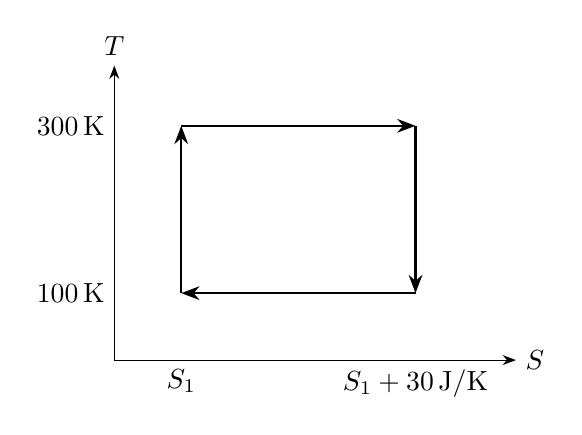
\begin{tikzpicture}[>=Stealth,scale=0.85]
\draw[->] (0,0)--(6,0) node[right] {$S$};
\draw[->] (0,0)--(0,4.4) node[above] {$T$};
\draw[->,thick] (1,3.5)--(4.5,3.5);
\draw[->,thick] (4.5,3.5)--(4.5,1);
\draw[->,thick] (4.5,1)--(1,1);
\draw[->,thick] (1,1)--(1,3.5);
\node[left] at (0,3.5) {$300\,\mathrm K$};
\node[left] at (0,1) {$100\,\mathrm K$};
\node[below] at (1,0) {$S_1$};
\node[below] at (4.5,0) {$S_1+30\,\mathrm{J/K}$};
\end{tikzpicture}
\end{center}
\crosscheck T--S矩形面积 $(300-100)\times30=6000$ J；每循环工作物质熵变为零。
\sourceproblem{10-T13}{65}{69}
\problemtext 0.5 kg、0摄氏度冰置于恒温20摄氏度的大热源，最终变为20摄氏度水；求刚融完和随后升温阶段的熵变。熔化热335 kJ/kg，水比热4180 J/(kg K)。
\workings 取 $T_m=273.15$ K、$T_H=293.15$ K。用可逆参考路径，
\[
\Delta S_1=\frac{m\lambda}{T_m}\approx613.22\,\mathrm{J/K},\quad
\Delta S_2=mc\ln\frac{T_H}{T_m}\approx147.69\,\mathrm{J/K}.
\]
总物质熵增约760.90 J/K。
\crosscheck 真实过程存在有限温差而不可逆；计算熵差仍可用同端点可逆路径。第二阶段不应简单用热量除以20摄氏度。
\sourceproblem{10-T14}{65}{69}
\problemtext 接上题，求热源熵变及冰水与热源整体的总熵变。
\workings 恒温热源放热 $Q=m\lambda+mc(20)=209300$ J，故 $\Delta S_H=-209300/293.15\approx-713.97$ J/K。整体熵变
\[
\Delta S_{\rm tot}=\frac{m\lambda}{T_m}+mc\ln\frac{T_H}{T_m}-\frac Q{T_H}\approx46.93\,\mathrm{J/K}.
\]
\crosscheck 总熵增为正，符合不可逆传热；热源温度保持恒定是大热源近似。

\section{第11组：机械振动}
\sourceproblem{11-T1}{66}{70}
\problemtext 总电荷 $Q>0$、半径 $R$ 的均匀带电球沿直径有细隧道，质量 $m$、电荷 $-q$ 的质点沿隧道运动，证明简谐振动并求周期。
\workings 忽略极细隧道去掉的电荷，均匀实心球内 $E_x=Qx/(4\pi\varepsilon_0R^3)$。质点满足 $m\ddot x=-qQx/(4\pi\varepsilon_0R^3)$，因此
\[
\omega=\sqrt{\frac{qQ}{4\pi\varepsilon_0mR^3}},\qquad
T=2\pi\sqrt{\frac{4\pi\varepsilon_0mR^3}{qQ}}.
\]
\crosscheck 要求振幅不超过球内有效区间且隧道足够细；有限宽孔破坏球对称，不能无条件使用完整球场。
\sourceproblem{11-T2}{66}{70}
\problemtext 竖直弹簧劲度 $k$ 支撑质量 $M$ 的光滑平板，板上质量 $m$ 的物块被水平入射质点击中并离板，求板之后的振动。
\workings 采用题意的瞬时卸载且无竖向冲量模型。以卸载后的平衡位置为原点、向上为正，初位移 $x_0=-mg/k$，初竖向速度0。卸载后 $M\ddot x=-kx$，所以
\[
x(t)=-\frac{mg}{k}\cos\left(\sqrt{k/M}\,t\right).
\]
\crosscheck 若物块离板需要有限时间，碰后附加质量也可能暂时加载，初始条件须由离板时刻确定；题目未给板宽及停留时间，上式为瞬时卸载的标准解。
\sourceproblem{11-T3}{67}{71}
\problemtext 竖直弹簧 $k=500$ N/m，原悬物 $M=4$ kg；质量 $m=1$ kg 的黏性物自下方0.6 m以4 m/s上抛，击中后粘合，取 $g=10$，求振动方程及最大拉力。
\workings 碰前速度 $u=\sqrt{4^2-2(10)(0.6)}=2$ m/s向上。短时碰撞后共同速度 $v_0=mu/(M+m)=0.4$ m/s。新平衡位置在自然端点下0.10 m，原平衡位置在其下0.08 m，故以新平衡为原点、向上为正，$x_0=0.02$ m，$\omega=\sqrt{500/5}=10$ rad/s。
\[
x(t)=0.02\cos10t+0.04\sin10t,\quad
A=\sqrt{0.02^2+0.04^2}=0.04472\,\mathrm m.
\]
最大拉力 $F_{\max}=500(0.10+A)\approx72.36$ N。
\crosscheck 碰撞阶段用动量而非机械能守恒；若用自然长端点为坐标原点，位移为 $x(t)-0.10$ m；初始速度和加速度回代一致。
\sourceproblem{11-T4}{67}{71}
\problemtext 质量 $m$ 的物体经无滑动轻绳绕半径 $R$、惯量 $J$ 的定滑轮接劲度 $k$ 的弹簧，从平衡点下拉小距离释放，证明简谐振动并求角频率。
\workings 取平衡位置向下位移为 $x$，绳长约束使弹簧伸长增量等于 $x$，滑轮角速度为 $\dot x/R$。平衡后的重力与预拉伸线性势能项抵消，机械能
\[
E=\tfrac12(m+J/R^2)\dot x^2+\tfrac12kx^2.
\]
由运动方程 $(m+J/R^2)\ddot x+kx=0$ 得 $\omega=\sqrt{k/(m+J/R^2)}$。
\crosscheck 绳须始终绷紧；$J\to0$ 恢复普通弹簧振子频率。
\sourceproblem{11-T5}{68}{72}
\problemtext 竖直弹簧振子振幅0.24 m、周期4 s，初始在平衡位置下0.12 m向上运动，质量1 kg；求振动式、首次到达上方0.12 m的时间、该处合力。
\workings 取向上正，$\omega=\pi/2$，初相位取 $-2\pi/3$，故 $x=0.24\cos(\pi t/2-2\pi/3)$ m。首次达到 $+0.12$ m 时相位为 $-\pi/3$，故 $t=2/3$ s。合力 $F=-m\omega^2x=-0.03\pi^2$ N，约0.296 N向下。
\crosscheck 初速为正，且该相位为初相位之后最早满足目标位移的解。
\sourceproblem{11-T6}{68}{72}
\problemtext 图示简谐振动初位移 $5.65\times10^{-2}$ m，首次正最大位移在1 s，负最大在5 s，求振动式及10 s时位移、速度、加速度。
\workings 由半周期4 s得 $T=8$ s、$\omega=\pi/4$。取 $x=A\cos[\pi(t-1)/4]$，$A=0.0565/\cos(\pi/4)=0.0565\sqrt2$ m，约0.0799 m。10 s时相位 $9\pi/4$，故
\[
x=0.0565\,\mathrm m,\quad v=-0.0565\pi/4\approx-0.0444\,\mathrm{m/s},\quad
a=-0.0565(\pi/4)^2\approx-0.0349\,\mathrm{m/s^2}.
\]
\crosscheck 图示初速度为正；10 s等价于2 s，位移正、速度和加速度负。

\section{第13组：光的干涉}
\sourceproblem{13-T1}{79}{83}
\problemtext 同频同初相相干光在折射率n的均匀介质内传播，两路几何路程差为 $r_2-r_1$，求光程差和相位差。
\workings $\Delta L=n(r_2-r_1)$，传播相位滞后差 $\Delta\phi=2\pi\nu\Delta L/c$。若定义同一时刻第二束的相位减第一束，则为 $-2\pi\nu\Delta L/c$。
\crosscheck 真空波长 $\lambda_0=c/\nu$；不重复乘折射率。
\sourceproblem{13-T2}{79}{83}
\problemtext 600 nm光由空气斜入射折射率1.23、厚1 cm平板再出射，入射角30度，板外两段各5 cm，求介质中频率、速率、波长及总几何路程与光程。
\workings $\nu=c/\lambda_0=5.00\times10^{14}$ Hz，$u=c/1.23\approx2.439\times10^8$ m/s，$\lambda=600/1.23\approx487.8$ nm。折射角满足 $\sin r=0.5/1.23$，板内路径 $L=1/\sqrt{1-(0.5/1.23)^2}$ cm，约1.0945 cm。几何路程 $10+L\approx11.095$ cm，光程 $10+1.23L\approx11.346$ cm。
\crosscheck 折射前后频率不变，板内路径并非板厚；空气折射率近似为1。
\sourceproblem{13-T3}{79}{83}
\problemtext 双缝间距0.30 mm、屏距1.20 m，第五暗纹距中央11.39 mm，求波长。
\workings 第五暗纹对应 $(5-1/2)\lambda$。近轴 $\lambda=dx/(4.5D)\approx6.328\times10^{-7}$ m，即约633 nm。用远场角度修正 $\lambda=d x/[4.5\sqrt{D^2+x^2}]$，结果约632.75 nm。
\crosscheck 第一暗纹对应半波长而非一波长；近轴角约0.00949 rad。

\section{第14组：量子物理}
\sourceproblem{14-T1}{93}{97}
\problemtext 概述普朗克解释黑体辐射的假设及其与经典物理的差异。
\workings 振子能量取离散值 $E_n=nh\nu$（经典普朗克表述），能量交换以 $h\nu$ 的整数倍进行；经典理论允许能量连续改变，并以均分得到紫外发散。量子假设导出平均热能 $h\nu/[\exp(h\nu/k_BT)-1]$，抑制高频辐射。
\crosscheck 现代量子谐振子含零点能；该常数不改变这里的平均热激发能。
\sourceproblem{14-T2}{93}{97}
\problemtext 用能量和动量守恒证明孤立自由电子不能完全吸收单个非零能量光子。
\workings 在初电子静止系，光子能量 $\epsilon>0$，动量 $\epsilon/c$。若仅剩电子，$E_f=m_ec^2+\epsilon,\ p_f=\epsilon/c$。质量壳条件要求 $E_f^2-p_f^2c^2=m_e^2c^4$，展开却为 $m_e^2c^4+2m_ec^2\epsilon$，矛盾。
\crosscheck 结论由洛伦兹不变量保证任意惯性系均成立；束缚电子可由原子或其他物体承担反冲。
\sourceproblem{14-T3}{93}{97}
\problemtext 波长700 nm、25 pm、1.24 pm的三种光子，求能量、动量及教材质量记号。
\workings $E=hc/\lambda,\ p=h/\lambda,\ m_{\rm eq}=E/c^2$。取 $h=6.62607015\times10^{-34}$ J s、$c=2.99792458\times10^8$ m/s，三组按 $(E,p,m_{\rm eq})$ 顺序约为
\[
\begin{array}{ccc}
2.84\times10^{-19}&9.47\times10^{-28}&3.16\times10^{-36}\\
7.95\times10^{-15}&2.65\times10^{-23}&8.84\times10^{-32}\\
1.60\times10^{-13}&5.34\times10^{-22}&1.78\times10^{-30}
\end{array}
\]
单位依次为J、kg m/s、kg。
\crosscheck 三种光子不变质量均为零；最后一列仅为教材相对论质量或能量等效质量，不是静质量。原页指数已放大确认。
\sourceproblem{14-T4}{94}{98}
\problemtext 能量0.60 MeV的X光康普顿散射后波长增大20\%，求电子增加能量。
\workings $E'=E/1.2=0.50$ MeV，能量守恒给反冲动能增加 $0.10$ MeV。
\crosscheck 能量与波长反比，不能直接以20\%乘初能量。
\sourceproblem{14-T5}{94}{98}
\problemtext 入射光子波长3.0 pm，反冲电子速率0.6c，求散射光子波长和散射角。
\workings 电子初静止，$\gamma=1.25$，$K=(\gamma-1)m_ec^2\approx127.75$ keV。$E_0=hc/\lambda\approx413.28$ keV，$E'=E_0-K\approx285.53$ keV，$\lambda'=hc/E'\approx4.342$ pm。由康普顿公式 $\cos\phi=1-(\lambda'-\lambda)/(h/m_ec)$，得 $\phi\approx63.5^\circ$。
\crosscheck 波长增量约1.342 pm小于两倍康普顿波长4.852 pm；使用相对论动能而非经典公式。
\sourceproblem{14-T6}{95}{99}
\problemtext 氢原子由第n轨道跃迁至第二轨道，光波长487 nm，求第n轨道半径。
\workings 里德伯公式 $1/\lambda=R_H(1/4-1/n^2)$，代入得到 $n\approx4$（波长为近似值）。玻尔半径关系 $r_n=n^2a_0$，故 $r_4\approx8.47\times10^{-10}$ m。
\crosscheck 精确整数能级对应约486 nm；按题目数据精度识别n，而不把非整数反解当作轨道量子数。
\sourceproblem{14-T7}{95}{99}
\problemtext 远处速率 $1.875\times10^6$ m/s的电子被质子俘获形成基态氢，求释放光子频率。
\workings 在固定质子、忽略反冲的教材模型，$h\nu=\tfrac12m_ev^2+13.6\,\mathrm{eV}$，电子初动能约10.0 eV，故 $\nu\approx5.71\times10^{15}$ Hz。
\crosscheck 原页速度指数为6；实际有限质子质量使部分能量进入氢原子反冲，精确频率应结合总动量守恒与初始质子速度。

\section{第15组：物质波与量子力学基础}
\sourceproblem{15-T1}{96}{100}
\problemtext 静质量 $6.68\times10^{-27}$ kg、速率5000 km/s的alpha粒子，求德布罗意波长。
\workings $\lambda=h/p$，非相对论近似 $p=mv$，$v=5.00\times10^6$ m/s，故 $\lambda\approx1.984\times10^{-14}$ m；精确式为 $h/(\gamma mv)$，$\gamma=(1-v^2/c^2)^{-1/2}$。
\crosscheck 相对论修正约0.014\%，不影响题给有效数字。
\sourceproblem{15-T2}{96}{100}
\problemtext 中子质量 $1.67\times10^{-27}$ kg，分别取3 K与300 K的典型热运动动能 $3k_BT/2$，求物质波长。
\workings $p=\sqrt{3mk_BT}$，$\lambda=h/\sqrt{3mk_BT}$。两温度下分别约 $1.45\times10^{-9}$ m与 $1.45\times10^{-10}$ m。
\crosscheck 室温中子实际具有速率分布，第二问取同一平均动能标度，不是所有中子的波长相同。
\sourceproblem{15-T3}{97}{101}
\problemtext 电子和光子波长均0.20 nm，分别求动量及动能。
\workings 共同动量 $p=h/\lambda\approx3.313\times10^{-24}$ kg m/s。光子能量 $pc\approx9.93\times10^{-16}$ J，即6.20 keV；电子动能 $K=\sqrt{p^2c^2+m_e^2c^4}-m_ec^2\approx6.02\times10^{-18}$ J，即37.6 eV，可近似为 $p^2/(2m_e)$。
\crosscheck 波长相同只保证动量相同；两者色散关系不同。
\sourceproblem{15-T4}{97}{101}
\problemtext 铀核尺度 $L=7.2\times10^{-15}$ m，估算核中alpha粒子动量、动能和电子最低动能尺度。
\workings 取教材数量级估计 $\Delta x\sim L,\ p\sim\hbar/L=1.46\times10^{-20}$ kg m/s。alpha粒子（质量 $6.7\times10^{-27}$ kg）非相对论动能约 $1.60\times10^{-14}$ J，即0.100 MeV。电子必须使用相对论公式，$pc\approx27.4$ MeV，$K=\sqrt{(pc)^2+(m_ec^2)^2}-m_ec^2\approx26.9$ MeV。若以标准差不等式 $\Delta x\Delta p\ge\hbar/2$ 并取 $\Delta x=L$，对应动量下界尺度减半，alpha动能尺度约0.0250 MeV，电子约13.2 MeV。
\crosscheck 不确定关系约束标准差，不确定核尺度定义及量子态时无法由此给出严格最低本征能；上述为局域化动量和能量的估算，不能将电子用经典动能公式计算。
\sourceproblem{15-T5}{98}{102}
\problemtext 氦氖激光波长632.8 nm，谱宽 $10^{-9}$ nm，估算纵向位置不确定度或波列长度。
\workings $p=h/\lambda$，窄谱下 $\Delta p\simeq h\Delta\lambda/\lambda^2$。若以谱宽的倒数定义相干长度标度，$L_c\simeq\lambda^2/\Delta\lambda=400.44$ m。若两宽度均按标准差定义，$\sigma_x\sigma_p\ge\hbar/2$ 给 $\sigma_x\ge\lambda^2/(4\pi\sigma_\lambda)\approx31.9$ m（将题给谱宽视为标准差）。
\crosscheck 谱线宽度的定义与波列形状决定数值因子，原题不能给出唯一精确长度；原页指数为负9，单位为nm。
\sourceproblem{15-T6}{98}{102}
\problemtext 以不确定关系估计氢原子基态结合能和第一玻尔半径。
\workings 采用三维尺度估算 $p\sim\hbar/r$，令 $C=k_ee^2$，则 $E(r)\sim\hbar^2/(2m_er^2)-C/r$。求极小值 $E'(r)=0$ 得 $r=\hbar^2/(m_e C)=a_0\approx5.29\times10^{-11}$ m，$E_{\min}\sim-m_e C^2/(2\hbar^2)\approx-13.6$ eV，结合能约13.6 eV。若按严格一维标准差下界直接以 $\hbar/2$ 替代尺度动量中的 $\hbar$，会得半径四分之一及结合能四倍，说明该替代不是严格求氢原子基态的方法。
\crosscheck 该尺度法恰给玻尔模型数值并非由一维不确定不等式严格推出；固定核、库仑势及非相对论模型下的精确本征值应由薛定谔方程求解。
\sourceproblem{15-T7}{99}{103}
\problemtext 无限深势阱 $0\le x\le a$ 内波函数 $\psi=A\sin(3\pi x/a)$，求归一化、概率密度及最大概率密度的位置。
\workings $1=|A|^2\int_0^a\sin^2(3\pi x/a)dx=|A|^2a/2$，可取 $A=\sqrt{2/a}$（整体相位任意）。$\rho(x)=2\sin^2(3\pi x/a)/a$，阱外为零。峰值 $2/a$ 出现在 $a/6,a/2,5a/6$。
\crosscheck 阱壁满足零边界条件；连续分布中单点概率为零，所求实际是概率密度的峰。
\sourceproblem{15-T8}{99}{103}
\problemtext 无限深势阱定态 $\psi=\sqrt{2/a}\sin(n\pi x/a)$，求在0至 $a/3$ 区间发现粒子的概率。
\workings 对 $n=1,2,\ldots$，
\[
P=\frac2a\int_0^{a/3}\sin^2(n\pi x/a)dx
=\frac13-\frac{\sin(2n\pi/3)}{2n\pi}.
\]
\crosscheck $n=3j$ 时恰为1/3，大n极限也为1/3；原题未给具体n，保留通式。

\section{第16组：固体能带与激光}
\sourceproblem{16-T1}{104}{108}
\problemtext 从能带结构说明绝缘体与半导体导电性能差异。
\workings 理想本征材料在零温时价带满、导带空。半导体禁带较窄，有限温度热激发可产生导带电子与价带空穴，载流子浓度有 $\exp[-E_g/(2k_BT)]$ 的主要温度依赖；绝缘体通常禁带较宽，同温度下热激发载流子很少。
\crosscheck 能隙并非唯一因素，迁移率、杂质、缺陷、温度均影响实际电导；没有对所有材料都适用的严格能隙分界值。
\sourceproblem{16-T2}{104}{108}
\problemtext 本征半导体锗禁带宽0.67 eV，估算太阳电池带间吸收的最大波长。
\workings 光子能量需满足 $hc/\lambda\ge E_g$，故 $\lambda_{\max}=hc/E_g\approx1.85$ 微米。
\crosscheck 是能量阈值估计；锗为间接带隙材料，实际带边吸收还涉及声子和跃迁概率。
\sourceproblem{16-T3}{105}{109}
\problemtext 解释粒子数反转及实现的必要条件。
\workings 对激光跃迁上、下能级，反转条件为 $N_u/g_u>N_l/g_l$（$g$ 为简并度），等简并时为 $N_u>N_l$。正常正温热平衡不满足该条件，须由外界泵浦建立非平衡分布，并使抽运及弛豫机制能够维持反转。
\crosscheck 粒子数反转只给受激净增益的必要基础；持续激光振荡还要求增益克服损耗。
\sourceproblem{16-T4}{105}{109}
\problemtext 说明激光器的主要组成和光学谐振腔作用。
\workings 通常包括增益介质、泵浦系统和光学反馈谐振腔。谐振腔提供多次通过增益介质的反馈，选择满足相位和损耗条件的模式，并经部分透射镜输出光。稳态振荡须满足往返净增益补偿损耗。
\crosscheck 泵浦供能，谐振腔本身不产生能量；无腔放大器也能有受激辐射，但不等同于通常的谐振腔激光振荡器。

\section{第17组：原子核与核物理}
\sourceproblem{17-T1}{106}{110}
\problemtext 钴60源每秒测得3700个伽马光子，测量效率10\%，半衰期5.27年，求活度与质量。
\workings 令每次衰变计入测量的平均光子数为 $Y$，光子探测效率 $\eta=0.10$，则 $A=3700/(\eta Y)=3.70\times10^4/Y$ Bq。$N=AT_{1/2}/\ln2$，$m=NM/N_A$，取 $M=0.060$ kg/mol，得到 $m\approx8.85\times10^{-13}/Y$ kg。教材若取一次衰变计一个光子或效率已按每次衰变定义，则 $Y=1$；若两个级联光子均计数且各自效率10\%，近似 $Y=2$，活度和质量均减半。
\crosscheck 活度是核衰变次数率，不是光子计数率；原题未说明能窗和光子产额，保留条件解。
\sourceproblem{17-T2}{106}{110}
\problemtext 10 kg的天然铀氧化物 $U_3O_8$ 中估计镭226、镤231含量，给定铀同位素丰度和两子核半衰期。
\workings 取化学式纯物质模型，铀原子总数 $N_U=3(10\,\mathrm{kg})N_A/M_{U_3O_8}$，用原子丰度 $f_{238}=0.9927,f_{235}=0.0072$。若矿物封闭且长衰变链达到长期平衡，则子核与相应母核活度相等，
\[
N_{\rm Ra}=f_{238}N_U T_{\rm Ra}/T_{238},\quad
N_{\rm Pa}=f_{235}N_U T_{\rm Pa}/T_{235}.
\]
质量分别为 $N_{\rm Ra}M_{\rm Ra}/N_A,N_{\rm Pa}M_{\rm Pa}/N_A$。题给子核半衰期1600年和 $3.27\times10^4$ 年，母核半衰期未在本题列出，故保留参数式。
\crosscheck 实际矿石的纯度、年龄、化学迁移及衰变链平衡状态影响含量；未达平衡时仅凭铀丰度不能确定子核存量。
\sourceproblem{17-T3}{107}{111}
\problemtext 古木片燃烧得0.3 mol二氧化碳，碳14活度读数每分钟9次，估算年龄。
\workings 还原碳质量约3.6 g。设活体参考比活度 $a_0$（每克每分钟衰变次数），效率 $\eta$，半衰期 $T_{1/2}$，则 $9=\eta(3.6)a_0\,2^{-t/T_{1/2}}$，故
\[
t=\frac{T_{1/2}}{\ln2}\ln\frac{3.6\eta a_0}{9}.
\]
若读数已校正为真实活度、取 $\eta=1$，仍需参考比活度与半衰期才能代入。
\crosscheck 原题没有给初始参考活度和计数效率；实际年代还需本底、同位素分馏及校准曲线等修正，不能凭给定读数唯一确定年龄。
\sourceproblem{17-T4}{107}{111}
\problemtext 太阳含氢 $1.5\times10^{30}$ kg，光度 $3.9\times10^{26}$ W，以恒功率估算氢燃尽时间。
\workings 设可参与聚变的氢比例为f，转为所计辐射能的质量比例为 $\epsilon$，则 $t=f\epsilon Mc^2/P$。取教材理想全部氢燃烧 $f=1$、氢聚变为氦的近似质量亏损 $\epsilon=0.007$，得到 $t\approx2.42\times10^{18}$ s，即约 $7.67\times10^{10}$ 年。
\crosscheck 不可把全部氢静能直接当作辐射能；真实太阳只有部分氢能参与主序阶段核心聚变，光度也会变化，故本数值不是太阳真实剩余寿命。

\chapter{常州工学院《大学物理学习指导》}
\section{第1章：质点运动学（1.5练习题）}
\sourceproblem{选择1}{8}{14}
\problemtext 以时针为参照，求分针相对转动一周的周期。
\workings 相对角速度为 $2\pi(1/60-1/720)\,\mathrm{rad/min}$，故周期 $720/11=65\tfrac5{11}\,\mathrm{min}$，选 B。
\crosscheck 相对周期应大于分针对表盘的 $60\,\mathrm{min}$ 周期。
\sourceproblem{选择2}{8}{14}
\problemtext 半径 $R$ 的圆周走完一周，求途中最大位移模及最大累计路程。
\workings 最大弦长为直径 $2R$，累计路程最大为周长 $2\pi R$，选 C。
\crosscheck 回到起点的最终位移为零，不是途中位移最大值。
\sourceproblem{选择3}{8}{14}
\problemtext $x=t^2-4t+5$（SI），求最初 $3\,\mathrm s$ 的位移及路程。
\workings $v=2t-4$，在 $t=2\,\mathrm s$ 换向。$x(0)=5$，$x(2)=1$，$x(3)=2$，因此 $\Delta x=-3\,\mathrm m$，$s=|1-5|+|2-1|=5\,\mathrm m$，选 D。
\crosscheck 路程大于位移的模；分段积分 $|v|$ 得相同数值。
\sourceproblem{选择4}{8}{14}
\problemtext 识别二维位矢所对应的速度大小。
\workings $v=|\dot{\bm r}|=\sqrt{\dot x^2+\dot y^2}$，选 D。径向距离的变化率 $\mathrm d|\bm r|/\mathrm dt$ 通常不等于速率；$\dot{\bm r}$ 是矢量。
\crosscheck 匀速圆周运动的径向距离不变，但速率非零；亦排除只用径向变化率的表达式。
\sourceproblem{选择5}{8}{14}
\problemtext 比较曲线运动的速度、速率及其时间平均。
\workings 瞬时 $|\bm v|=v$；平均量满足
\[
|\bar{\bm v}|=\frac{|\int\bm v\,\mathrm dt|}{\Delta t}
\le\frac{\int|\bm v|\,\mathrm dt}{\Delta t}=\bar v.
\]
若所考察区间确含速度方向改变，则严格小于，按通常曲线运动题意选 C。
\crosscheck 原题的“必定”需限定区间：若只截取同向直线段，则可取等号。等号条件为非零速度几乎处处同向；不把一般不等式误写成无条件严格不等式。
\sourceproblem{选择6}{8}{14}
\problemtext $x=t^3+5t+6$（SI），判别直线运动。
\workings $v=3t^2+5>0$，$a=6t$。按通常从 $t=0$ 起计、$t>0$ 的时间域，加速度正向且随时变化，选 C。
\crosscheck 若允许负时间，加速度方向反转；$t=0$ 时加速度为零。应明确时间域。
\sourceproblem{选择7}{8}{14}
\problemtext $x=at,\ y=b+ct^2$，速度与 $x$ 轴成 $45^\circ$ 时求速率。
\workings $\bm v=a\bm i+2ct\bm j$，此时 $|2ct|=|a|$，所以 $v=\sqrt2|a|$；原选项 B 对应通常 $a>0$ 的约定。
\crosscheck $a$ 与 $c$ 均不得导致速度方向条件无解；常数符号未明示，严格结果应保留绝对值。
\sourceproblem{选择8}{8}{14}
\problemtext 岸高 $h$，绳经岸上定滑轮以恒定速率 $u>0$ 收取，判断船的运动。
\workings 令船距岸脚的水平距离为 $x>0$，斜绳长 $\ell=\sqrt{x^2+h^2}$，$\dot\ell=-u$，故
\[
\dot x=-u\ell/x,\qquad \ddot x=-u^2h^2/x^3.
\]
在 $h>0$ 时速度及加速度同向，船加速靠岸，选 C（加速但非匀加速）。
\crosscheck 以上为绳绷紧、忽略滑轮尺寸及船高的几何模型；$h=0$ 退化为匀速。$x\to0$ 的发散表明理想模型适用边界。

\section{第2章：牛顿定律（2.5练习题）}
\sourceproblem{选择1}{23}{29}
\problemtext 轻弹簧悬物随手向上匀加速，手突然停止的瞬间判断物体运动。
\workings 弹簧长度及物体速度在瞬间连续，原先张力 $T=m(g+a)$，故停止瞬间物体仍向上且加速度为原来的 $a>0$，选C。
\crosscheck 手的速度突变不等于弹簧下端物体速度突变；后续运动不一定持续匀加速。
\sourceproblem{选择2}{23}{29}
\problemtext 电梯静止时秤读500牛，匀变速时400牛，求加速度。
\workings 质量 $m=500/g$，向上取正，$ma=400-500=-100\,\mathrm N$，故 $a=-0.2g$，选C。
\crosscheck 秤读是支持力大小，减小表明加速度向下，不表明速度方向。
\sourceproblem{选择3}{23}{29}
\problemtext 图3竖直圆顶点A沿不同弦静止无摩擦下滑，比较耗时。
\workings 设弦与竖直夹角 $\theta$，弦长 $s=2R\cos\theta$，沿弦加速度 $g\cos\theta$。由 $s=at^2/2$ 得 $t=2\sqrt{R/g}$，两弦相同，选A。
\crosscheck 适用于非退化弦，起点为圆的最高点。
\sourceproblem{选择4}{23}{29}
\problemtext 质点沿圆弧匀速率下滑，判断合力与切向力。
\workings $a_\tau=0$，合切向力为零；法向合力为 $mv^2/R$，随运动转向，选C。
\crosscheck 合力大小恒定并不意味着合力矢量不变。
\sourceproblem{选择5}{23}{29}
\problemtext 水平光滑台上质量 $m_B$ 经轻绳连悬物 $m_A$；改用恒力 $m_Ag$ 直接拉绳，比较加速度。
\workings 原系统 $a=m_Ag/(m_A+m_B)$，新系统 $a'=m_Ag/m_B>a$，选B。
\crosscheck 悬物本身需要加速，原绳张力小于其重力；假定滑轮理想。
\sourceproblem{选择6}{23}{29}
\problemtext 图6两等质量物体由竖直压缩轻弹簧连接，下方平板C突然抽去，求瞬间加速度大小（图在PDF30）。
\workings 原先上方A受向上弹力 $mg$；抽板瞬间弹簧形变不变，A合力仍零；B受向下弹力 $mg$ 和重力 $mg$，故 $a_A=0,a_B=2g$（B向下），选C。
\crosscheck 原图是压缩弹簧，不是悬挂拉伸弹簧；平板的支持力只在抽板前存在。
\sourceproblem{选择7}{24}{30}
\problemtext 两同质量者从同高度静止沿理想轻绳两端攀爬，相对绳速率不同，比较到达顶点的情况。
\workings 轻绳和无摩擦轻滑轮使两侧张力相同；两人各有 $m\ddot y=T-mg$，因此相同初始条件下地面系高度和速度始终相同，到同一顶点同时，选C。
\crosscheck 相对绳速度不同可以由绳本身运动补偿；结论要求持续满足相同张力与相等质量。
\sourceproblem{选择8}{24}{30}
\problemtext 水平运动货车在恒牵引力 $F$ 下持续接收竖直落煤，判断速度与加速度趋势。
\workings 设车及已装煤质量 $M(t)$，落煤入射水平速度零，则 $F=\mathrm d(Mv)/\mathrm dt$，故
\[
a=\frac{F-\dot Mv}{M}.
\]
即使假设恒质量流率 $q>0$，$v=(M_0v_0+Ft)/(M_0+qt)$，$a=M_0(F-qv_0)/(M_0+qt)^2$。若 $F>qv_0$，速度增大、正加速度减小（A）；若 $F<qv_0$，速度减小、负加速度趋零（若指大小则减小）。相等时匀速。
\crosscheck 原题未给质量流率和初始速度关系，不能无条件唯一选择；且加速度有向值与大小应区分。
\sourceproblem{选择9}{24}{30}
\problemtext 某星球质量为地球的0.1倍、半径0.5倍，求表面重力加速度。
\workings 忽略自转，$g'=GM'/R'^2=(0.1/0.5^2)g=0.4g$，选A。
\crosscheck 半径按平方反比计，不直接按质量比计算。
\sourceproblem{选择10}{24}{30}
\problemtext 圆轨道航天器内宇航员离开舱体，判断运动。
\workings 若离舱时与航天器同位置近似、同速度且无额外推力，重力提供同样向心加速度，宇航员继续沿近似相同的圆轨道运动，选C。
\crosscheck 若离舱具有额外相对速度，轨道一般不再严格相同；教材选项默认无额外冲量。
\sourceproblem{选择11}{24}{30}
\problemtext 单摆摆长 $l$，速度大小 $v$，摆角 $\theta$，求加速度大小。
\workings 切向分量 $a_\tau=-g\sin\theta$（取摆角增大为正），法向分量 $a_n=v^2/l$，故 $a=\sqrt{v^4/l^2+g^2\sin^2\theta}$，选C。
\crosscheck 不依赖小角近似；在最低点切向加速度为零。
\sourceproblem{选择12}{24}{30}
\problemtext 圆锥摆绳长 $l$，与竖直夹角 $\theta$，求转动周期。
\workings 张力 $S$ 满足 $S\cos\theta=mg$、$S\sin\theta=m\omega^2l\sin\theta$，非退化圆锥摆有 $\omega^2=g/(l\cos\theta)$，$T=2\pi\sqrt{l\cos\theta/g}$，选D。
\crosscheck $0<\theta<\pi/2$；不能将静止垂直摆直接当作圆锥轨道。
\sourceproblem{选择13}{24}{30}
\problemtext 半径 $R$ 的旋转竖直圆筒内壁物块，静摩擦系数 $\mu$，求不下滑的最低角速度（选项及图在PDF31）。
\workings 法向支持力 $N=m\omega^2R$，静摩擦需平衡 $mg$，因此 $mg\le\mu m\omega^2R$，$\omega_{\min}=\sqrt{g/(\mu R)}$，选C。
\crosscheck $\mu>0$；应用静摩擦上限而非假设摩擦总等于 $\mu N$。
\sourceproblem{选择14}{25}{31}
\problemtext 半球碗半径0.10米，球在距碗底0.04米处水平匀速圆周运动，求角速度。
\workings 设法线与竖直夹角 $\theta$，$\cos\theta=(R-h)/R=0.6$；$N\cos\theta=mg,N\sin\theta=m\omega^2R\sin\theta$，故 $\omega=\sqrt{g/(R-h)}\approx12.8\,\mathrm{rad/s}$，选B。
\crosscheck 不需先求水平圆半径；取 $g=9.8$，近似13弧度每秒。
\sourceproblem{选择15}{25}{31}
\problemtext 水平面上滑动摩擦系数 $\mu$，固定大小的拉力 $F$ 斜向上，求使水平加速度最大的角度。
\workings 保持接触且向右滑动时 $N=mg-F\sin\theta$，$ma=F(\cos\theta+\mu\sin\theta)-\mu mg$。无约束最大值在 $\tan\theta=\mu$，选B。
\crosscheck 该角须满足 $F\sin\theta\le mg$；若不满足，则须在可接触角度域上求边界最优，不能让支持力为负。静止起动还需静摩擦条件。
\sourceproblem{选择16}{25}{31}
\problemtext 水平弯道半径 $R$，轮胎与地面静摩擦系数 $\mu$，求不侧滑的速率条件。
\workings $mv^2/R\le\mu mg$，故 $v\le\sqrt{\mu gR}$，选B。
\crosscheck 默认没有同时纵向加速或制动，且路面水平；质量约去。
\sourceproblem{选择17}{25}{31}
\problemtext $x=x_0\sin\omega t$，求质量 $m$ 的物体所受合力。
\workings $a=\ddot x=-\omega^2x$，所以 $f=-m\omega^2x$，选D。
\crosscheck 负号表示回复力，量纲为牛顿。
\sourceproblem{选择18}{25}{31}
\problemtext 质量10千克，$F=(120t+40)\bm i$（SI），初速度 $6\bm i$，求3秒速度。
\workings $a=12t+4$，积分得 $v=6+6t^2+4t$，故 $\bm v(3)=72\bm i\,\mathrm{m/s}$，选C。
\crosscheck 冲量为 $\int_0^3(120t+40)\,\mathrm dt=660\,\mathrm{N\,s}$，动量增量相符。
\sourceproblem{选择19}{25}{31}
\problemtext 同上力与质量，初位置负10米、初速度6米每秒，求1秒位置。
\workings $x=-10+6t+2t^3+2t^2$，故 $x(1)=0$，选B。
\crosscheck 两次微分给定加速度，初始条件均成立。
\sourceproblem{选择20}{25}{31}
\problemtext 质量 $m$ 物体下落，阻力大小 $kv^2$，求终端速率。
\workings 取向下为正，$m\dot v=mg-kv^2$，稳态 $\dot v=0$，得 $v_\infty=\sqrt{mg/k}$，选A。
\crosscheck $k>0$，单位为质量除以长度；正根对应下落速度大小。

\section{第3章：动量守恒定律和能量守恒定律（3.5练习题）}
\sourceproblem{选择1}{39}{45}
\problemtext 20克小物体以500米每秒嵌入木块，碰后速度50米每秒，求木块受冲量。
\workings 小物体动量变化 $0.020(50-500)=-9\,\mathrm{N\,s}$；按相互作用冲量等大反向，木块受向前9牛秒冲量，选A。
\crosscheck 忽略其他水平冲量；碰后木块动量增加。
\sourceproblem{选择2}{40}{46}
\problemtext 质量 $m$ 的锤以向下速率 $v$ 撞桩，作用时间 $\Delta t$，重力不可忽略，求平均冲力。
\workings 若碰撞结束时锤静止，取向上为正，$\bar F\Delta t-mg\Delta t=mv$，故 $\bar F=mv/\Delta t+mg$，选A。
\crosscheck 完全非弹性碰撞本身只意味着共同末速度，并不保证静止；若末态仍向下速率 $u$，应为 $m(v-u)/\Delta t+mg$。教材选A需补充静止条件。
\sourceproblem{选择3}{40}{46}
\problemtext 质量 $m$ 的质点速率 $v$ 不变、速度方向转过 $\theta$，求净冲量大小。
\workings $I=|\Delta\bm p|=mv\sqrt{2-2\cos\theta}=2mv\sin(\theta/2)$（$0\le\theta\le\pi$），选A。
\crosscheck 方向改变即动量改变，即使动能不变。
\sourceproblem{选择4}{40}{46}
\problemtext 8千克静止物体受4牛秒净冲量，求速度大小。
\workings $v=I/m=0.5\,\mathrm{m/s}$，选A。
\crosscheck 速度方向与冲量方向一致；题目只给冲量大小。
\sourceproblem{选择5}{40}{46}
\problemtext 静止质量 $M$ 的核分出质量 $m$、速率 $v_0$ 的粒子，经典模型下求余部反冲速率。
\workings 若余部质量为 $M-m$，动量守恒得 $(M-m)v_{\rm recoil}=mv_0$，故 $v_{\rm recoil}=mv_0/(M-m)$，选A。
\crosscheck 采用教材经典质量加和近似；相对论衰变中静质量通常不守恒，需知道余部静质量并使用四动量。
\sourceproblem{选择6}{40}{46}
\problemtext 静水中船长 $L$，人与船质量相等，人由船尾走到船头，求船位移。
\workings 令船位移 $X$，人相对地面位移 $X+L$。水平质心不变，$mX+m(X+L)=0$，故 $X=-L/2$，选C。
\crosscheck 船的位移与人相对船的行走方向相反。
\sourceproblem{选择7}{40}{46}
\problemtext 静止船上两不同质量的人相向行走，判断船运动方向。
\workings 以地面系动量为准，$\bm p_{\rm boat}=-(\bm p_1+\bm p_2)$。若两人地面系动量反向且大小不等，船沿较小动量者的运动方向，选B。
\crosscheck 两人若仅给相对船的速度，需先转换参考系；若动量大小相等则船瞬时静止。
\sourceproblem{选择8}{40}{46}
\problemtext 圆锥摆在水平面内匀速率转动，判断重力和张力做功。
\workings 重力竖直，张力位于竖直径向平面，均与瞬时切向位移垂直，因此各自功为零，选A。
\crosscheck 张力水平分量虽提供向心力，但不改变动能。
\sourceproblem{选择9}{40}{46}
\problemtext 理想弹簧从自然长先拉伸5厘米，再额外拉伸5厘米，比较两段准静态外力功。
\workings $W_1=k(0.05)^2/2$，$W_2=k[(0.10)^2-(0.05)^2]/2=3W_1$，故 $W_1<W_2$，选C。
\crosscheck 若题设没有明确初始自然长，仍在初始伸长非负的线性区时后段功更大；假定准静态。
\sourceproblem{选择10}{40}{46}
\problemtext 均匀链长 $h$、质量 $m$，将下端提至上端使链对折悬挂，求外力准静态功。
\workings 初质心低于悬点 $h/2$，末质心低于悬点 $h/4$，故 $W=mg(h/2-h/4)=mgh/4$，选B。
\crosscheck 不应将整条链当作均升高 $h/2$ 的质点。
\sourceproblem{选择11}{41}{47}
\problemtext 摆长 $l$、质量 $m$，水平外力将小球缓慢从最低点移至摆角 $\theta$ 处，求功。
\workings 准静态动能不变，绳张力不做功，故外力功等于重力势能增量 $mgl(1-\cos\theta)$，选C。
\crosscheck 水平拉力通常随摆角变化，不能直接用恒力公式 $Fs$。
\sourceproblem{选择12}{41}{47}
\problemtext 比较一对作用与反作用力的冲量和功。
\workings 同一时段内 $\bm I_1=-\bm I_2$，非零时矢量不同；两力作用点位移可不同，功不必相等，选D。
\crosscheck 例：滑动接触的两物体相互摩擦功之和通常为负。零冲量为退化情形。
\sourceproblem{选择13}{41}{47}
\problemtext 弹簧原长 $l_0$，从长度 $l_1$ 伸至 $l_2$，求弹性力功。
\workings 伸长量 $x=l-l_0$，故 $W=-\int_{l_1-l_0}^{l_2-l_0}kx\,\mathrm dx=-k[(l_2-l_0)^2-(l_1-l_0)^2]/2$，选C。
\crosscheck 力与继续伸长方向相反，功为负。
\sourceproblem{选择14}{41}{47}
\problemtext 质量10千克、速度 $8\bm i+3\bm j$（m/s），求动能。
\workings $K=10(8^2+3^2)/2=365\,\mathrm J$，选C。
\crosscheck 速度分量须先平方求和。
\sourceproblem{选择15}{41}{47}
\problemtext 轮船阻力与速率平方成正比，稳定航行速率翻倍，求所需推进功率之比。
\workings 匀速时牵引力等于阻力 $kv^2$，机械功率 $P=kv^3$，翻倍后为8倍，选D。
\crosscheck 发动机输入功率还取决于推进效率；教材默认效率不变。
\sourceproblem{选择16}{41}{47}
\problemtext 质量10千克，速度 $\bm v=4t^2\bm i+16\bm j$（SI），求1至2秒合外力功。
\workings $W=\Delta K=5[(16^2+16^2)-(4^2+16^2)]=1200\,\mathrm J$，选B。
\crosscheck 亦可积分 $m\dot{\bm v}\cdot\bm v=320t^3$，结果相同。
\sourceproblem{选择17}{41}{47}
\problemtext 判断质点动量、动能、合外力冲量与功的逻辑关系。
\workings 若合外力冲量为零，$\Delta\bm p=0$，固定质量质点的 $\Delta K=0$，故合外力功为零，选C。反向不成立，因为速度方向可能变化。
\crosscheck 圆周运动半周内合力不做功却有非零冲量；必须将外力理解为合外力。
\sourceproblem{选择18}{41}{47}
\problemtext 质点从同一P点静止沿光滑固定斜面或圆弧到同一Q点，比较末动量和动能。
\workings 重力势能下降相同，约束力不做功，末速率相同；图中两条轨迹在Q处切线方向不同，故末动量矢量不同、动能相同，选D。
\crosscheck 结论依赖原图终点切线不同；若切线相同则动量也相同。
\sourceproblem{选择19}{41}{47}
\problemtext 小物体嵌入水平光滑地面上的静止木块，辨别动能损失、阻力功和生热关系（选项续PDF48）。
\workings 对入射小物体应用动能定理，其动能减少等于克服木块阻力所做的功（假定水平作用为唯一做功项），选C。系统机械能损失等于两物体总动能减少，而非入射物体单独动能减少。
\crosscheck 木块动能增加，故小物体损失的动能不全转为热，也不全转为木块动能；实际内能增加可包含形变等。
\sourceproblem{选择20}{42}{48}
\problemtext 比较圆锥摆、理想斜抛、光滑斜面自由下滑、外力牵引匀速上升四种机械能变化。
\workings 前三项在教材理想条件下机械能守恒；牵引匀速上升时动能不变而重力势能增加，外力做正功，选D。
\crosscheck 系统为物体与地球，外牵引力的功改变系统机械能。
\sourceproblem{选择21}{42}{48}
\problemtext 两物体从等高水平桌面经压缩弹簧弹出，水平射程 $s_1=s_2/2$，求质量关系。
\workings 下落时间相同，所以 $v_1=v_2/2$。弹出过程中水平动量守恒，$m_1v_1=m_2v_2$，因此 $m_1=2m_2$，选A。
\crosscheck 射程正比于初水平速率；不是正比于动能。
\sourceproblem{选择22}{42}{48}
\problemtext 竖直弹簧挂球静态伸长 $d$，由弹簧原长处静止释放，求最大伸长。
\workings $mg=kd$，最大伸长 $x$ 处速率为零，$mgx=kx^2/2$，非零根为 $x=2d$，选C。
\crosscheck 振动中心为 $d$，振幅为 $d$。
\sourceproblem{选择23}{42}{48}
\problemtext 两球完全非弹性碰撞后共同静止，比较碰前动量。
\workings 总动量为零，故 $\bm p_1=-\bm p_2$，大小相等方向相反，选D。
\crosscheck 动能为 $p^2/(2m)$，质量不同时动能不必相等。
\sourceproblem{选择24}{42}{48}
\problemtext 地球沿椭圆轨道由近日点至远日点，判断功、动能、势能及机械能变化。
\workings 距离 $r$ 增大，$U=-GMm/r$ 增大，中心引力做负功，动能减小，总机械能不变，选C。
\crosscheck 忽略其他天体扰动及非保守作用。
\sourceproblem{选择25}{42}{48}
\problemtext 孤立的质子与另一带电粒子发生库仑散射，判断系统守恒量。
\workings 教材采用静电保守相互作用、忽略辐射的两体模型，系统无外力，动量与机械能均守恒，选D。
\crosscheck 更完整的电动力学中若计辐射，须把电磁场及辐射的能量和动量纳入封闭系统；不能仅用粒子机械量声称精确守恒。

\section{第4章：刚体的转动（4.5练习题）}
\sourceproblem{选择1}{56}{62}
\problemtext 定轴匀变速转动时距轴 $r$ 的点，比较切向和法向加速度的变化。
\workings $a_\tau=r|\alpha|$ 恒定，$a_n=r\omega^2$ 随 $\omega=\omega_0+\alpha t$ 变化，选C。
\crosscheck 取 $r>0,\alpha\ne0$；轴上点两分量均为零。
\sourceproblem{选择2}{56}{62}
\problemtext 两力作用于定轴刚体，判断合力与轴向力矩的逻辑关系。
\workings 平行轴的力对该轴力矩必为零，所以原A所说的“可能为零”也成立；垂直轴的两力也可使轴向力矩抵消，B成立。C、D分别可用力偶、通过轴线的合力反驳。
\crosscheck 严格按可能性的逻辑，A和B均真；若原意是区分必然与可能，应将A改成“可能不为零”等明确措辞。
\sourceproblem{选择3}{56}{62}
\problemtext 判断刚体内力矩、作用反作用力矩及相等质量刚体运动的命题（选项续PDF63）。
\workings 在教材经典中心内力假设下，$\bm\tau_{12}+\bm\tau_{21}=(\bm r_1-\bm r_2)\times\bm F_{12}=0$，选B。内力矩不改变整体轴向角动量；等质量不保证等惯量。
\crosscheck 若只假设作用反作用力等大反向、不假设沿两作用点连线，则力矩和可能非零，B须注明中心力条件。
\sourceproblem{选择4}{57}{63}
\problemtext 光滑定轴刚体受多个合力为零的力，判断转速。
\workings 轴向力矩可为零或非零，$\alpha=\tau_z/J$，所以转速可能不变也可能改变，选D。
\crosscheck 力偶的合力为零但力矩非零。
\sourceproblem{选择5}{57}{63}
\problemtext 匀质杆由水平静止绕端轴下摆，比较角速度及角加速度大小。
\workings 设下摆角 $\phi$，$\alpha=3g\cos\phi/(2l)$、$\omega^2=3g\sin\phi/l$，故角速率增大而角加速度大小减小，选C。
\crosscheck 最低点重力矩为零但角速率最大。
\sourceproblem{选择6}{57}{63}
\problemtext 飞轮绕绳挂质量 $m$ 重物时角加速度为 $\alpha$，改用恒拉力 $2mg$，比较新角加速度。
\workings 半径 $R$、惯量 $J$ 时 $\alpha=mgR/(J+mR^2)$，新值 $\alpha'=2mgR/J>2\alpha$，选C。
\crosscheck 原绳张力小于 $mg$，不是直接施加重力大小的恒力。
\sourceproblem{选择7}{57}{63}
\problemtext 相同定滑轮A受恒力 $Mg$，B挂质量 $M$ 重物，比较角加速度。
\workings $\alpha_A=MgR/J$，$\alpha_B=MgR/(J+MR^2)$，故 $\alpha_A>\alpha_B$，选B。
\crosscheck 理想无滑动及无轴摩擦。
\sourceproblem{选择8}{57}{63}
\problemtext 转动惯量取决于哪些因素。
\workings $J=\int r_\perp^2\,\mathrm dm$，取决于质量、分布、转轴位置和方向，选C。
\crosscheck 与转速无关。
\sourceproblem{选择9}{57}{63}
\problemtext 同半径同质量细环，一个质量均匀一个不均匀，比较中心垂直轴惯量。
\workings 各质量元轴距均为 $R$，故两者均为 $mR^2$，选C。
\crosscheck 转轴通过几何环心，不一定通过非均匀环质心。
\sourceproblem{选择10}{57}{63}
\problemtext 长 $l$、质量 $m$ 的匀质杆两端各有质量 $m$ 的小球，求中心垂直轴惯量。
\workings $J=ml^2/12+2m(l/2)^2=7ml^2/12$，选A。
\crosscheck 小球视作质点，系统质心仍位于中点。
\sourceproblem{选择11}{57}{63}
\problemtext 等质量等厚度两圆盘，$\rho_A>\rho_B$，比较半径与惯量（选项续PDF64）。
\workings $m=\rho\pi R^2h$，故 $R_A<R_B$；$J=mR^2/2$，故 $J_A<J_B$，选C。
\crosscheck 固定质量和厚度时惯量与密度成反比。
\sourceproblem{选择12}{58}{64}
\problemtext 判断角动量守恒的充分必要条件。
\workings 在惯性系取固定参考点，$\mathrm d\bm L/\mathrm dt=\bm\tau_{\rm ext}$，故合外力矩为零是充要条件，选B。
\crosscheck 若仅讨论固定轴分量，条件应是合外力矩的轴向分量为零，而非全部矢量必须为零。
\sourceproblem{选择13}{58}{64}
\problemtext 质点受有心力，判断何种力学量守恒。
\workings 对力心的力矩为零，角动量守恒，选C。
\crosscheck 有心力未必是时间无关的保守力，动能及势能也通常变化。
\sourceproblem{选择14}{58}{64}
\problemtext 自由转台上的人收回哑铃，判断机械能及角动量。
\workings 若把转台、人、哑铃整体计入，轴向外力矩为零，角动量守恒；惯量减小使 $K=L_z^2/(2J)$ 增加，机械能不守恒，选C为教材预期。
\crosscheck 原题只称人与哑铃系统，若转台具有惯量且可交换角动量，则该子系统角动量不一定守恒；严格表述应包含转台或说明其惯量可忽略。
\sourceproblem{选择15}{58}{64}
\problemtext 光滑铰链悬杆绕竖轴转动，小环沿杆下滑，判断杆环系统轴向角动量及含地球系统机械能。
\workings 若初始转动后系统自由演化，固定铰点不做功、重力对竖轴力矩为零，故机械能与轴向角动量均守恒，选D。
\crosscheck 若“匀角速”指外部驱动始终维持角速度恒定，则驱动可施加外力矩并做功，上述守恒不再自动成立；答案D采用自由演化解释。
\sourceproblem{选择16}{58}{64}
\problemtext 图示转盘受两个等大反向非共线力，判断转速变化。
\workings 图中原角速度为顺时针，力偶上方作用线向右、下方作用线向左，产生顺时针力矩，故角速率增大，选A。
\crosscheck 必须按两条力的作用线而非合力判定；图示方向保留复核标记。
\sourceproblem{选择17}{58}{64}
\problemtext 两等质量入射质点速度等大反向共线，分别嵌入转盘，比较碰后角速率。
\workings 两入射质点的轴向角动量之和为零，而碰后惯量增加，故由角动量守恒可知角速率减小，选C。
\crosscheck 原转速非零，嵌入位置距轴非零；不使用机械能守恒。
\sourceproblem{选择18}{58}{64}
\problemtext 自由定轴转动物体发生热膨胀或冷收缩，判断角速率（选项续PDF65）。
\workings 在通常均匀各向同性变形模型下，膨胀使轴距增大、惯量增大，角速率减小；收缩相反，选D。
\crosscheck 若变形仅沿轴向，惯量可不变，因此须注明径向尺寸变化的条件。
\sourceproblem{选择19}{59}{65}
\problemtext 惯量 $J$ 的水平转台初角速度 $\omega_0$，质量 $m$ 的人由中心沿径向到半径 $R$ 的边缘，求末角速度。
\workings 以人为质点，轴向角动量守恒，$\omega=J\omega_0/(J+mR^2)$，选A。
\crosscheck 假设人在转台系无额外切向相对速度；初末角动量均需包括人。
\sourceproblem{选择20}{59}{65}
\problemtext 匀质细杆长 $l$，由自然下垂位置获得初角速率，求持续绕端轴转动的条件。
\workings 质心到倒立位置升高 $l$，能量阈值由 $ml^2\omega^2/6=mgl$ 得 $\omega_c=\sqrt{6g/l}$。严格连续越过倒立点须 $\omega>\omega_c$，原选项C为阈值表达。
\crosscheck 等号时倒立点速度趋零，理想模型中趋近该点所需时间发散，不属于持续整周转动。
\sourceproblem{选择21}{59}{65}
\problemtext 长 $2l$、质量 $m$ 的细杆中心固定，质量 $m$ 小球以速率 $v$ 垂直撞击杆端并粘合，求末角速度。
\workings $mvl=(ml^2/3+ml^2)\omega$，故 $\omega=3v/(4l)$，选C。
\crosscheck 轴向角动量守恒，碰撞机械能损失为正。
\sourceproblem{选择22}{59}{65}
\problemtext 轻杆长20厘米，两球初始距中心各5厘米，烧断约束线后滑至杆端，求角速度。
\workings 无轴向外力矩，$J_i\omega_0=J_f\omega$，半径增为2倍，惯量变4倍，故 $\omega=\omega_0/4$，选D。
\crosscheck 角动量守恒不表示角速度恒定；此为球刚到杆端前的瞬时值。
\sourceproblem{选择23}{59}{65}
\problemtext 长 $5/3$ 米的匀质杆从与向下竖直成60度处静止释放，取 $g=10$，求最大角速率。
\workings $\tfrac12(ml^2/3)\omega^2=mg(l/2)(1-\cos60^\circ)$，故 $\omega=\sqrt{3g/(2l)}=3\,\mathrm{rad/s}$，选A。
\crosscheck 最低点势能最小；杆长为原页分数 $5/3$ 米。
\sourceproblem{选择24}{59}{65}
\problemtext 长 $L$、质量 $M$ 的杆绕端轴静止，质量 $m$ 的入射质点垂直穿过自由端，速度由 $v$ 降为 $v/2$，求杆角速率（续PDF66）。
\workings 短时轴向角动量守恒，$mvL-m(v/2)L=(ML^2/3)\omega$，得 $\omega=3mv/(2ML)$，选C。
\crosscheck 假设穿出方向不变；不使用机械能守恒。
\sourceproblem{选择25}{60}{66}
\problemtext 自转者收臂使转动惯量降为原来的三分之一，求角速度及动能。
\workings $J_0\omega_0=(J_0/3)\omega$，故 $\omega=3\omega_0$；$K=L_z^2/(2J)$，故 $K=3K_0$，选D。
\crosscheck 机械能增加来自内部做功。
\sourceproblem{选择26}{60}{66}
\problemtext 同长同质量单摆和端轴匀质杆由相同偏角静止释放，比较最低点角速率。
\workings 单摆 $\omega_1^2=2g(1-\cos\theta)/l$；杆 $\omega_2^2=3g(1-\cos\theta)/l$，故非零偏角时 $\omega_1<\omega_2$，选C。
\crosscheck 两者质心高度差和转动惯量不同；$\theta=0$ 时均为零。
\sourceproblem{选择27}{60}{66}
\problemtext 两同质量同平动速率球，一个无自转、另一个有自转，比较将其完全停止所做的功。
\workings 若指使两球平动和转动均停止的合外力总功，则 $W_1=-mv^2/2$，$W_2=-mv^2/2-J\omega^2/2$，故 $W_1>W_2$，选A。若比较克服运动的功的绝对值，则反向不等。
\crosscheck 若只停止质心而不停止自转，或只问手的功而另有耗散路径，须另给模型。
\sourceproblem{选择28}{60}{66}
\problemtext 惯量 $J$ 的圆盘角速率由 $\omega_0$ 降为 $\omega_0/2$，求阻力矩做功。
\workings 若阻力矩为唯一做功的力矩，$W=\Delta K=J(\omega_0^2/4-\omega_0^2)/2=-3J\omega_0^2/8$，选B。
\crosscheck 阻力矩做负功；有驱动力矩时不能仅由动能差确定阻力功。
\sourceproblem{选择29}{60}{66}
\problemtext 椭圆轨道卫星在远地点A和近地点B，比较角动量及动能。
\workings 中心引力对地心力矩为零，故 $L_A=L_B$；近远地点速度垂直径矢，$R_Av_A=R_Bv_B$，$R_A>R_B$ 时 $K_B>K_A$，选A。
\crosscheck 圆轨道退化情形两动能相等；题设最大最小距离不同。

\sourceproblem{填空1}{61}{67}
\problemtext 恒角加速度圆盘由 $20\pi$ 增至 $30\pi$ rad/s，期间转60圈，求角加速度及历时。
\workings $\Delta\theta=120\pi$，$\alpha=(\omega_2^2-\omega_1^2)/(2\Delta\theta)=25\pi/12\,\mathrm{rad/s^2}$，$\Delta t=(\omega_2-\omega_1)/\alpha=4.8\,\mathrm s$。
\crosscheck 平均角速率 $25\pi$ 乘4.8秒为 $120\pi$。
\sourceproblem{填空2}{61}{67}
\problemtext 飞轮初角速率5 rad/s，20秒后降为初值0.8倍，求恒角加速度及100秒转角。
\workings $\alpha=(4-5)/20=-0.05\,\mathrm{rad/s^2}$，$\theta=5(100)-0.025(100)^2=250\,\mathrm{rad}$。
\crosscheck 100秒恰好停止，区间内没有反向转动。
\sourceproblem{填空3}{61}{67}
\problemtext 皮带传动主动轮半径0.1米、1450转每分，从动轮半径0.29米，求从动轮缘速率和转速。
\workings 不打滑时 $v=2\pi(0.1)(1450/60)\approx15.18\,\mathrm{m/s}$；$n_2=1450(0.1/0.29)=500\,\mathrm{r/min}$。
\crosscheck 两轮缘线速率相同，角速率不同。
\sourceproblem{填空4}{61}{67}
\problemtext $\theta=10+8t-5t^2$（SI），求0.2秒角速度、角加速度及距轴0.5米点的速度和切法向加速度。
\workings $\omega=8-10t=6$，$\alpha=-10$（SI），$v=3\,\mathrm{m/s}$，$a_\tau=-5\,\mathrm{m/s^2}$（以正转向为正），$a_n=18\,\mathrm{m/s^2}$。
\crosscheck 切向加速度大小为5，法向指向轴。
\sourceproblem{填空5}{61}{67}
\problemtext $\omega=2+t+3t^2$，求0.2秒角速度及角加速度。
\workings $\omega=2.32\,\mathrm{rad/s}$，$\alpha=1+6t=2.2\,\mathrm{rad/s^2}$。
\crosscheck 角加速度是角速度的一阶导数。
\sourceproblem{填空6}{61}{67}
\problemtext 半径0.5米滑轮牵引升降机以0.4米每平方秒加速上升，求角加速度大小。
\workings 无滑动时 $|\alpha|=a/r=0.8\,\mathrm{rad/s^2}$。
\crosscheck 方向由绕绳方向确定。
\sourceproblem{填空7}{61}{67}
\problemtext 飞轮600转每分、惯量2.5，恒力矩制动1秒停止，求力矩大小。
\workings $\omega_0=20\pi$，$|M|=J\omega_0/t=50\pi\,\mathrm{N\,m}$。
\crosscheck 制动力矩方向与初始角速度相反。
\sourceproblem{填空8}{61}{67}
\problemtext 惯量2.0的轮受恒力矩负7.0牛米，8秒后角速度为初值的相反数，求初角速度。
\workings $\alpha=-3.5$，$-\omega_0=\omega_0-3.5(8)$，故 $\omega_0=14\,\mathrm{rad/s}$。
\crosscheck 4秒停止后反向加速，8秒末角速度为负14。
\sourceproblem{填空9}{61}{67}
\problemtext 惯量50的系统从静止0.5秒匀加速至 $4\pi$ rad/s，求0.3秒角速率及驱动力矩。
\workings $\alpha=8\pi$，$\omega(0.3)=2.4\pi\,\mathrm{rad/s}$，$M=400\pi\,\mathrm{N\,m}$。
\crosscheck 驱动力矩等于合力矩须忽略其他阻力矩。
\sourceproblem{填空10}{61}{67}
\problemtext 球惯量 $5\times10^{-2}$，$\theta=2+4t-t^2$，求首次停止时间和外力矩大小。
\workings $\omega=4-2t$，故 $t=2\,\mathrm s$；$\alpha=-2$，$|M|=0.10\,\mathrm{N\,m}$。
\crosscheck 角速度零不表示角加速度零。
\sourceproblem{填空11}{61}{67}
\problemtext 质量 $m$ 的斜抛质点从O出发，初速 $v_0$、仰角 $\alpha$，求对O角动量、导数及力矩。
\workings 取纸外为正，$x=v_0t\cos\alpha,\ y=v_0t\sin\alpha-gt^2/2$。故
\[
L_z=m(xv_y-yv_x)=-mgv_0t^2\cos\alpha/2,\qquad
\dot L_z=M_z=-mgv_0t\cos\alpha.
\]
\crosscheck 直接计算重力矩 $-mgx$ 与导数一致。
\sourceproblem{填空12}{61}{67}
\problemtext 同质量 $m$ 同半径 $R$ 的细环与均匀圆盘，求中心垂直轴惯量（续PDF68）。
\workings 细环 $J=mR^2$，圆盘 $J=mR^2/2$。
\crosscheck 圆盘各质量元轴距小于等于 $R$，因此惯量较小。
\sourceproblem{填空13}{62}{68}
\problemtext 两等质量等身高者从静止沿轻绳两端攀爬，甲相对绳速度为乙两倍，比较到顶时间。
\workings 理想轻滑轮两端张力相等，两人质量相同，故地面系加速度、速度及高度始终相同（相同初高条件下），同时到达。
\crosscheck 相对绳速度不同由绳的运动补偿；若初高度不同，不能推出同时到达。
\sourceproblem{填空14}{62}{68}
\problemtext 500千克飞轮质量集中在半径0.6米轮缘，角速率220 rad/s，30秒匀减速停止，求惯量和制动力矩。
\workings $J=500(0.6)^2=180\,\mathrm{kg\,m^2}$，$|M|=180(220/30)=1320\,\mathrm{N\,m}$。
\crosscheck 质量集中于轮缘，不使用均匀圆盘的二分之一系数。
\sourceproblem{填空15}{62}{68}
\problemtext 飞轮20秒由40 rad/s匀减速至零，惯量50，求转角及力矩大小。
\workings $\theta=(40/2)20=400\,\mathrm{rad}$，$\alpha=-2$，$|M|=100\,\mathrm{N\,m}$。
\crosscheck 角速度时间图面积为400。
\sourceproblem{填空16}{62}{68}
\problemtext 长 $L$ 轻杆两端固定 $m,2m$，绕中点水平轴转动，从图示60度释放，求惯量、水平位置力矩及角加速度大小。
\workings $J=3mL^2/4$。水平位置重力矩大小 $(2m-m)gL/2=mgL/2$，故 $|\alpha|=2g/(3L)$。
\crosscheck 重球一侧下摆；两球重力矩方向相反。
\sourceproblem{填空17}{62}{68}
\problemtext 匀质杆长 $L$，水平静止释放，求初角速度和初角加速度。
\workings $\omega_0=0$，$J=mL^2/3$，$|\alpha_0|=mgL/(2J)=3g/(2L)$。
\crosscheck 初始角速度零而重力矩非零。
\sourceproblem{填空18}{62}{68}
\problemtext 匀质细杆长 $l$、质量 $m$，绕端轴由水平静止下摆角 $\theta$，求惯量和角速率。
\workings $J=ml^2/3$，$\frac12J\omega^2=mg(l/2)\sin\theta$，故 $\omega=\sqrt{3g\sin\theta/l}$。
\crosscheck $\theta=0$ 为初态，$\theta=\pi/2$ 为最低点。
\sourceproblem{填空19}{62}{68}
\problemtext 匀质杆水平静止释放，求初角加速度及竖直位置角速率。
\workings $\alpha_0=3g/(2l)$（下摆为正），$\omega_{\rm bottom}=\sqrt{3g/l}$。
\crosscheck 分别使用转动定律和机械能守恒。
\sourceproblem{填空20}{62}{68}
\problemtext 匀质杆长 $L$ 由竖直直立轻碰倒下，底端固定不滑动，求将达水平地面时角速率及角加速度大小。
\workings 取微扰极限，质心下降 $L/2$，$\omega=\sqrt{3g/L}$；水平位置 $|\alpha|=3g/(2L)$。
\crosscheck 精确直立且静止为不稳定平衡；结果为碰地前瞬时值，不涉及碰撞。
\sourceproblem{填空21}{62}{68}
\problemtext 匀质杆AB长 $l$，由水平静止下摆至角 $\theta$，求B端速率及重力矩功。
\workings $W=mg(l/2)\sin\theta$，$\omega^2=3g\sin\theta/l$，故 $v_B=\sqrt{3gl\sin\theta}$。
\crosscheck 不能将端点下降高度当作质心下降高度。
\sourceproblem{填空22}{62}{68}
\problemtext 恒轴向力矩 $M$ 作用于角速度 $\omega$ 的刚体，求瞬时功率及之后转两圈的功。
\workings 采用有向量，$P=M\omega$，若沿正方向转两圈，$W=4\pi M$。
\crosscheck 若转向与力矩反向，功为负；应采用有向转角。
\sourceproblem{填空23}{62}{68}
\problemtext 惯量 $J$ 的刚体受恒合力矩 $M$，求角加速度及角速度为 $\omega$ 时的功率。
\workings $\alpha=M/J$，$P=M\omega$。
\crosscheck 量纲分别为角度每平方秒和瓦。
\sourceproblem{填空24}{62}{68}
\problemtext 直径 $D$、质量 $m$ 的均匀飞轮从静止经时间 $t$ 被恒绳力加速至角速率 $\omega$，求角加速度及拉力功（续PDF69）。
\workings $\alpha=\omega/t$，$J=mD^2/8$，若忽略其他力矩做功，$W=J\omega^2/2=mD^2\omega^2/16$。
\crosscheck 也可由恒力矩 $J\alpha$ 乘转角 $\omega t/2$ 得到。
\sourceproblem{填空25}{63}{69}
\problemtext 地球两极冰融化后，判断地球惯量与自转速率的变化。
\workings 教材模型中质量由近轴区域向较大轴距分布，惯量增大；近似无外轴向力矩时 $\omega=L_z/J$ 减小。
\crosscheck 实际变化取决于水质量重新分布、地球形变及其他角动量交换，非仅由融化本身决定。
\sourceproblem{填空26}{63}{69}
\problemtext 惯量 $J$ 的圆盘受阻力矩 $-k\omega$，由 $\omega_0$ 减至一半，求时间和阻力矩功。
\workings $J\dot\omega=-k\omega$，$\omega=\omega_0e^{-kt/J}$，故 $t=J\ln2/k$，$W=-3J\omega_0^2/8$。
\crosscheck $k>0$；阻力矩为唯一做功项。
\sourceproblem{填空27}{63}{69}
\problemtext 惯量 $J_0$ 的飞轮以 $\omega_0$ 转动，与静止、惯量为其两倍的飞轮接合，求末角速度与动能变化。
\workings $\omega=\omega_0/3$，$\Delta K=(3J_0)(\omega_0/3)^2/2-J_0\omega_0^2/2=-J_0\omega_0^2/3$。
\crosscheck 轴向角动量守恒，机械能不守恒。
\sourceproblem{填空28}{63}{69}
\problemtext 光滑桌面小球质量 $m$，初始圆周半径 $r_1$、角速度 $\omega_1$，缓慢拉绳缩至 $r_2$，求动能增量。
\workings 角动量 $L=mr_1^2\omega_1$ 守恒，初末均为圆周运动时
\[
\Delta K=\frac{m r_1^2\omega_1^2}{2}\left(\frac{r_1^2}{r_2^2}-1\right).
\]
\crosscheck $r_2<r_1$ 时动能增加，由拉力做正功；若末态存在径向速度，须计入其动能。
\sourceproblem{填空29}{63}{69}
\problemtext 滑冰者惯量由 $J_0$ 减至 $2J_0/3$，初角速度 $\omega_0$，求末角速度及动能变化。
\workings $\omega=3\omega_0/2$，$K_f=(3/2)K_i$，故 $\Delta K=J_0\omega_0^2/4$。
\crosscheck 角动量守恒；增加的能量来自人体内部做功。
\sourceproblem{填空30}{63}{69}
\problemtext 长 $L$、质量 $M$ 的均匀杆由水平静止下摆，在竖直位置与静止质量 $m$ 物体完全非弹性碰撞，求碰后物体速率及对轴角动量。
\workings 碰前 $\omega_i=\sqrt{3g/L}$。若物体与杆端粘合，短时轴向角动量守恒给出
\[
\omega_f=\frac{M}{M+3m}\omega_i,\quad
v_m=\frac{M\sqrt{3gL}}{M+3m},\quad
|L_m|=mLv_m.
\]
\crosscheck 假设地面水平冲量可忽略、碰撞点在杆端；若物体未粘合或有其他外冲量矩，需重新建模。

\sourceproblem{计算1}{63}{69}
\problemtext 飞轮从静止6.0秒内匀加速至36 rad/s，求角加速度和转过圈数。
\workings $\alpha=36/6=6\,\mathrm{rad/s^2}$，$\theta=36(6)/2=108$ rad，$N=54/\pi\approx17.19$ 圈。
\crosscheck 角速度时间图面积为108 rad，不能将弧度直接当圈数。
\sourceproblem{计算2}{63}{69}
\problemtext 定轴运动 $\theta=at+bt^2-ct^4$，求角加速度及轴距 $r$ 点的切、法向加速度。
\workings $\omega=a+2bt-4ct^3,\alpha=2b-12ct^2$，$a_\tau=r(2b-12ct^2)$ 为沿正转向有向分量，$a_n=r(a+2bt-4ct^3)^2$。
\crosscheck 法向分量非负且指向轴；切向大小取绝对值。
\sourceproblem{计算3}{64}{70}
\problemtext 齿轮角加速度 $\alpha=4at^3-3bt^2$，初角速度 $\omega_0$，求角速度及转角。
\workings 积分得 $\omega=\omega_0+at^4-bt^3$，$\Delta\theta=\omega_0t+at^5/5-bt^4/4$。
\crosscheck 两次微分恢复给定角加速度；若发生反转，实际转过的总角路程须积分 $|\omega|$。
\sourceproblem{计算4}{64}{70}
\problemtext 均匀圆板半径 $R$、质量 $m$，在水平粗糙桌面绕中心轴转动，动摩擦系数 $\mu$，接触压力均匀，求摩擦力矩。
\workings 面压力 $p=mg/(\pi R^2)$，半径 $r$ 的环带摩擦力大小 $\mathrm dF=\mu p\,2\pi r\,\mathrm dr$，故
\[
|M_f|=\int_0^R r\,\mathrm dF=\frac23\mu mgR.
\]
方向与角速度相反。
\crosscheck 有效摩擦力臂为 $2R/3$，不是圆板质心的轴距零，也不是边缘半径。
\sourceproblem{计算5}{64}{70}
\problemtext 长 $l$、质量 $M$ 的均匀细杆绕端轴，另一端固定质量 $m$、半径 $r$ 的均匀实心小球，求系统惯量。
\workings 若杆端连接球面且球心在杆延长线上，轴到球心距 $l+r$，由平行轴定理
\[
J=Ml^2/3+2mr^2/5+m(l+r)^2.
\]
若 $l$ 指轴到球心的距离，则最后一项改为 $ml^2$，杆自身长度按实际取值。
\crosscheck 原图连接点与球心距离须区分；球质量分布若非均匀实心球，应另给质心惯量。
\sourceproblem{计算6}{64}{70}
\problemtext 圆柱半径 $R$，有四个贯通圆孔，孔半径 $R/3$，孔心距主轴 $R/2$，求中心轴惯量。
\workings 设未挖孔圆柱质量 $M_0$，每孔等效质量 $M_0/9$。若四孔互不重叠，则减去各孔惯量
\[
J=\frac12 M_0R^2-4\frac{M_0}{9}\left(\frac{R^2}{18}+\frac{R^2}{4}\right)=\frac{59}{162}M_0R^2.
\]
若题给 $m$ 是挖孔后质量，$m=5M_0/9$，则 $J=59mR^2/90$；若指完整圆柱质量，则取 $M_0=m$。
\crosscheck 相邻孔心距离 $R/\sqrt2>2R/3$，各孔不交叠；最外缘 $5R/6<R$，减法成立。原题质量含义需明示。
\sourceproblem{计算7}{65}{71}
\problemtext 实心圆柱质量16 kg、半径15 cm，轻绳悬8 kg物体，取 $g=10$，求张力及静止释放1秒下落距离。
\workings $J=Mr^2/2$，$mg-T=ma,\ T=Ja/r^2$，得 $a=mg/(m+M/2)=5\,\mathrm{m/s^2}$，$T=40$ N，$s=at^2/2=2.5$ m。
\crosscheck 张力小于悬物重力；半径在无滑动实心柱模型中约去。
\sourceproblem{计算8}{65}{71}
\problemtext 两质量 $m_1,m_2$ 分别悬在半径 $r,R$ 的同轴无质量鼓轮上，绳绕向相反，求角加速度。
\workings 取 $m_2$ 下降方向为正，$a_2=R\alpha,a_1=r\alpha$ 向上。消去两绳张力得
\[
\alpha=\frac{(m_2R-m_1r)g}{m_1r^2+m_2R^2}.
\]
\crosscheck 驱动力矩差为零时角加速度为零；若分子为负实际方向反转。
\sourceproblem{计算9}{65}{71}
\problemtext 光滑斜面倾角 $\theta$，物体质量 $m$ 经轻绳带动质量 $M$、半径 $R$ 的固定轴滑轮转动，求下滑加速度。
\workings $mg\sin\theta-T=ma,\ TR=Ja/R$，故 $a=mg\sin\theta/(m+J/R^2)$。若滑轮为均匀实心圆盘，$J=MR^2/2$，得 $a=mg\sin\theta/(m+M/2)$。
\crosscheck 题面仅给质量和半径，不足以唯一确定转动惯量；圆盘假设须明确。
\sourceproblem{计算10}{66}{72}
\problemtext 斜面30度、物体6 kg、悬物18 kg，均匀圆盘滑轮2 kg，斜面摩擦系数0.1，取 $g=10$，求加速度与两侧张力。
\workings 设悬物下降、斜面物体上行，$f=0.1(6)(10)\cos30^\circ=3\sqrt3$ N。
\[
a=\frac{180-30-3\sqrt3}{18+6+1}=\frac{150-3\sqrt3}{25}\approx5.792\,\mathrm{m/s^2}.
\]
斜面侧 $T_1=6a+30+3\sqrt3\approx69.95$ N；悬物侧 $T_2=180-18a\approx75.74$ N。
\crosscheck $T_2-T_1=a$（SI数值式），符合滑轮转动方程；取题给摩擦系数为滑动摩擦系数，启动需克服静摩擦。
\sourceproblem{计算11}{66}{72}
\problemtext 均匀圆盘原质量 $M$、半径 $R$，绕水平中心轴以角速度 $\omega$ 转动，边缘质量 $m$ 的碎块脱离并竖直上抛，求上升高度及余盘角动量。
\workings 若脱离无额外冲量，碎块初速 $R\omega$，相对脱离点最高上升 $h=R^2\omega^2/(2g)$。原盘角动量 $MR^2\omega/2$，碎块脱离瞬间角动量 $mR^2\omega$，故余盘 $L=(M/2-m)R^2\omega$。
\crosscheck 假设碎块尺寸可忽略且轴向外冲量矩为零；最高点绝对高度还需脱离点高度。
\sourceproblem{计算12}{66}{72}
\problemtext 匀质杆长 $l$，从水平上方60度静止释放，绕端轴下摆，$g=10$，求初角加速度与过水平时角速率。
\workings 下摆为正，初力矩 $mg(l/2)\cos60^\circ$，故 $\alpha_0=3g/(4l)=7.5/l$。质心到水平下降 $(l/2)\sin60^\circ$，能量守恒得 $\omega=\sqrt{3g\sin60^\circ/l}=\sqrt{15\sqrt3/l}$。
\crosscheck 初角加速度并非水平位置的 $3g/(2l)$；角速度由势能差求得。
\sourceproblem{计算13}{66}{72}
\problemtext 匀质水平杆质量 $m$、长 $l$，两端竖直细线悬挂，烧断一根，求另一根瞬时张力。
\workings 设保留端为A。初速度为零且细线不可伸长，A瞬时竖直加速度为零；杆此刻角加速度可按绕A求出，$mg(l/2)=(ml^2/3)\alpha$，故 $\alpha=3g/(2l)$。质心向下加速度 $\alpha l/2=3g/4$，因此 $mg-T=3mg/4$，$T=mg/4$。
\crosscheck 也可用质心转动方程 $Tl/2=(ml^2/12)\alpha$ 联立；A并非全过程固定铰点，此处仅用瞬时约束。

\section{第5章：静电场（5.5练习题）}
\sourceproblem{选择1}{80}{86}
\problemtext 两固定点电荷附近引入第三点电荷，判断原两者之间的相互作用力。
\workings 真空中点电荷之间的成对库仑力只取决于该对电荷及间距，故不变，选C。
\crosscheck 总合力一般变化；这里不考虑导体极化或原电荷位置改变。
\sourceproblem{选择2}{80}{86}
\problemtext 边长 $a$ 的立方体中心点电荷 $Q$，求顶点场强大小。
\workings 中心至顶点距离 $\sqrt3a/2$，故 $E=|Q|/(3\pi\varepsilon_0a^2)$，选C（按正电量约定）。
\crosscheck 场强大小非负，若 $Q<0$ 则方向向中心。
\sourceproblem{选择3}{80}{86}
\problemtext 原点正电荷 $Q$ 在 $(1,0)$ 产生场，求另一负电荷 $-2Q$ 的放置区域，使该点净场为零。
\workings 原场沿正x，负电荷必须在P左侧且共线，距离P为 $\sqrt2$（与坐标相同长度单位），故 $x=1-\sqrt2<0$，选C。
\crosscheck 仅匹配场强大小不足够，还须方向相反。
\sourceproblem{选择4}{80}{86}
\problemtext 半球开口平面与均匀电场平行，求曲面通量。
\workings 补底面后总通量为零，底面通量为零，故曲面通量也为零，选D。
\crosscheck 曲面各处场与法向夹角不同，不能直接用曲面积乘E。
\sourceproblem{选择5}{81}{87}
\problemtext 半球底面与均匀场夹30度，图中场有朝半球外侧的分量，求曲面外向通量。
\workings 底面外法向与场的夹角为120度，$\Phi_{\rm base}=-E\pi R^2/2$。闭合面净通量零，故 $\Phi_S=E\pi R^2/2$，选A。
\crosscheck 图中场箭头向右上，曲面净通量为正；若反转场方向则变号。
\sourceproblem{选择6}{81}{87}
\problemtext 立方体一顶点有点电荷 $q$，求图示不含电荷的对侧面通量。
\workings 拼合8个相同立方体使电荷在大立方体中心，每个大面通量 $q/(6\varepsilon_0)$，四个等价小面各得 $q/(24\varepsilon_0)$，选A。
\crosscheck 不直接对电荷位于边界的原立方体套内部电荷公式；以对称拼合规避奇点。
\sourceproblem{选择7}{81}{87}
\problemtext 两正点电荷相距 $2a$，以左电荷为中心作半径 $a$ 的高斯球，比较左右等面积小面元通量及总通量。
\workings 图中 $S_1$ 位于左端、$S_2$ 位于右端。中心电荷对两者贡献相等；右侧外电荷在左端的场沿外法向，在右端的场反外法向，因此 $\Phi_1>\Phi_2$；总通量 $q/\varepsilon_0$，选A。
\crosscheck 外部电荷不贡献闭合面净通量，却可改变局部通量。
\sourceproblem{选择8}{81}{87}
\problemtext 高斯面内电荷代数和为零，判断能确定的量。
\workings 高斯定理给 $\Phi_S=0$，仅此必然成立，选C。
\crosscheck 匀强场中任一闭面即为净通量零、局部场不为零的反例。
\sourceproblem{选择9}{81}{87}
\problemtext 判断关于高斯定理的四个推论。
\workings $\Phi=Q_{\rm enc}/\varepsilon_0$，若净内电荷非零则总通量非零，选D。净电荷为零不意味着内部无电荷；外场也可使面上各点场非零。
\crosscheck 对一般电场只由通量不能恢复逐点场强。
\sourceproblem{选择10}{81}{87}
\problemtext 无限长均匀带电圆柱面半径 $R$，辨认场强径向曲线（选项图在PDF88）。
\workings 轴对称高斯柱给出 $E=0$（$r<R$），$E=|\lambda|/(2\pi\varepsilon_0r)$（$r>R$），故在 $R$ 处跳变、外部反比衰减，选B。
\crosscheck 理想面电荷处场本身有两侧极限，不能当作连续体电荷。
\sourceproblem{选择11}{82}{88}
\problemtext 无限均匀正带电平面位于 $x=0$，辨认有向场强曲线。
\workings $E_x=(\sigma/2\varepsilon_0)\operatorname{sgn}(x)$，负半轴为负常量，正半轴为正同值常量，选C。
\crosscheck 平面处有跳变；电势连续。
\sourceproblem{选择12}{82}{88}
\problemtext 闭面包围点电荷Q，另一个点电荷由无穷远移到面外，判断总通量及面上场强。
\workings 净包围电荷不变，总通量仍为 $Q/\varepsilon_0$；外电荷场与原场叠加，一般使面上场强矢量改变，选D。
\crosscheck 外点电荷非零且位于有限距离时，其在面上任一点的场矢量均非零。
\sourceproblem{选择13}{82}{88}
\problemtext 图示非匀强场的电场线穿过球面，已知一小面通量 $\Delta\Phi_e$，求其余球面通量。
\workings 按图示球内无场线起止、无净电荷的教材意图，闭面总通量为零，故其余为 $-\Delta\Phi_e$，选A。
\crosscheck 若图仅是部分场线示意而并未给球内净电荷为零，则一般式为 $Q_{\rm enc}/\varepsilon_0-\Delta\Phi_e$，不能仅凭稀疏绘图证明无源。
\sourceproblem{选择14}{82}{88}
\problemtext 均匀带电球壳内总场为零，判断单个面元非零电荷在球内产生的场（选项续PDF89）。
\workings 在面元近似点电荷下，$\mathrm d\bm E=\mathrm dq\,\bm e_r/(4\pi\varepsilon_0r^2)$，球内任一点到面元距离有限且非零，因此不为零，选C。
\crosscheck 总场为零来自所有面元矢量叠加；假定 $\mathrm dq\ne0$。
\sourceproblem{选择15}{83}{89}
\problemtext 高斯面内净电荷为零时，判断面上场强。
\workings 总通量为零而场强不必处处为零，选C。反之总通量非零也不能保证面上每点的场强均非零。
\crosscheck 外部电场或内部等量异号电荷均可产生局部非零场。
\sourceproblem{选择16}{83}{89}
\problemtext 球面中心有点电荷，判断哪些操作改变闭面通量。
\workings 只有引入另一非零电荷到面内会改变净包围电荷，因此选B。
\crosscheck 移动内部点电荷或缩小仍包围它的球面不改变总通量。
\sourceproblem{选择17}{83}{89}
\problemtext 球对称场的图示为内区随半径线性上升、外区按平方反比下降，辨认电荷分布。
\workings 均匀体密度 $\rho$ 的实心球内 $E=|\rho|r/(3\varepsilon_0)$，外区 $E=|\rho|R^3/(3\varepsilon_0r^2)$，选B。
\crosscheck $\rho=Ar$ 对应内部二次函数，$\rho=A/r$ 对应内部常量（除中心奇点）；均不符合图示。
\sourceproblem{选择18}{83}{89}
\problemtext 正方形四顶点有等量电荷，中心场强和电势均为零，选符号排列。
\workings 取无穷远零势，四顶点至中心等距，电势为零要求两正两负。相对顶点同号时两对场分别抵消，故a、c为正、b、d为负的选项C正确。
\crosscheck 正负全部互换也成立；相邻顶点同号的排列净场非零。
\sourceproblem{选择19}{83}{89}
\problemtext 点电荷 $+q$ 至P距离 $a$，M距离 $2a$，以P为零势求M电势。
\workings $V_M=k_eq(1/(2a)-1/a)=-q/(8\pi\varepsilon_0a)$，选D。
\crosscheck P和M均在电荷右侧，远处电势低于近处。
\sourceproblem{选择20}{83}{89}
\problemtext 边长0.3 m的等边三角形两顶点分别带正负 $10^{-8}$ C，求第三顶点场强和电势（选项续PDF90）。
\workings 单个场强为 $9\times10^9(10^{-8})/0.3^2=1000$ V/m。两场夹120度，矢量和大小仍1000 V/m，方向平行正负电荷连线、由正指向负。电势等量反号抵消，$V=0$（无穷远零势），选B。
\crosscheck 电势是标量代数和，场强是矢量和。

\section{第6章：静电场中的导体与电介质（6.5练习题）}
\sourceproblem{选择1}{99}{105}
\problemtext 判断静电平衡带电导体的电势性质。
\workings 导体内部 $\bm E=0$，连通导体为等势体，表面同势，选D。
\crosscheck 曲率影响局部电荷密度，不意味着电势不同。
\sourceproblem{选择2}{99}{105}
\problemtext 正带电无限平面面密度 $\sigma$，旁放平行中性导体板，求近远两面感应面密度。
\workings 设近面 $\sigma_1$、远面 $\sigma_2$，中性给 $\sigma_1+\sigma_2=0$。板内场为零给 $\sigma+\sigma_1-\sigma_2=0$，得 $-\sigma/2,+\sigma/2$，选B。
\crosscheck 默认板孤立中性且无额外外场；若接地或另有净电荷，条件改变。
\sourceproblem{选择3}{99}{105}
\problemtext 半径R的接地导体球外距心2R有点电荷q，求感应净电荷。
\workings 镜像法等效球内像电荷 $q'=-qR/(2R)=-q/2$，位置距心 $R/2$，外部场满足球面零势；由包围球的高斯面知感应净电荷为 $-q/2$，选D。
\crosscheck 接地球可交换电荷，与孤立中性球不同。
\sourceproblem{选择4}{99}{105}
\problemtext 相距很远的半径R及r金属球用细导线连接，求面密度比。
\workings 忽略相互影响及导线电荷，等势给 $Q_R/R=Q_r/r$，故 $\sigma_R/\sigma_r=r/R$，选D。
\crosscheck 电荷量与半径成正比，面密度与半径成反比。
\sourceproblem{选择5}{99}{105}
\problemtext 孤立导体球半径R、电势 $U_0$，求球外轴距r处场强大小（选项续PDF106）。
\workings $V(r)=RU_0/r$，故 $E=R|U_0|/r^2$，按正电势约定选C。
\crosscheck 场强大小须非负，若 $U_0<0$ 方向向内。
\sourceproblem{选择6}{100}{106}
\problemtext 同轴导体内半径a、接地外筒半径b，内线密度正 $\lambda$，求间隙r处场与势。
\workings $E=\lambda/(2\pi\varepsilon_0r)$，$V=\int_r^b E(s)ds=\lambda\ln(b/r)/(2\pi\varepsilon_0)$，选D。
\crosscheck $V(b)=0$，负梯度恢复场。
\sourceproblem{选择7}{100}{106}
\problemtext 均匀带电无限厚导体板两侧等距离h处，比较电势差。
\workings 无额外外场的对称模型中两侧场强大小相同，且板为等势体，因此距板两侧相等距离处电势相等，选A。
\crosscheck 若外场破坏对称性，则不能仅凭距离相同得出等势。
\sourceproblem{选择8}{100}{106}
\problemtext 判断介质中高斯定理的正确推论。
\workings $\oint\bm D\cdot d\bm S=Q_{\rm free,enc}$，净通量只由包围的自由电荷代数和确定，选C。
\crosscheck 面上D为零仅能推出净自由电荷为零，不能排除等量异号自由电荷。
\sourceproblem{选择9}{100}{106}
\problemtext 导体球外充满相对介电常量 $\varepsilon_r$ 的均匀介质，测表面附近场强E，求自由面电荷密度。
\workings 取外法向，$D_n=\sigma_f$，若题设正电荷，则 $\sigma_f=\varepsilon_0\varepsilon_r E$，选B。
\crosscheck 一般有向式 $\sigma_f=\varepsilon_0\varepsilon_r\bm E\cdot\bm n$；大小用绝对值。
\sourceproblem{选择10}{100}{106}
\problemtext 空气平行板电容器中平行插介质板，比较介质场E和空气场 $E_0$。
\workings 忽略边缘效应且界面无自由电荷，法向D连续，$E=E_0/\varepsilon_r$；普通介质 $\varepsilon_r>1$，方向相同，选C。
\crosscheck 这里是沿场方向分层，并非并排介质的同电压情形。
\sourceproblem{选择11}{100}{106}
\problemtext 点电荷旁非对称放置介质，对以电荷为中心的球面判断高斯定理适用性。
\workings 高斯定理仍成立，但非对称极化破坏球对称，单凭积分定理不能推出球面逐点场强，选B。
\crosscheck $\bm E$ 通量涉及全部电荷，$\bm D$ 通量涉及自由电荷；二者均不因对称性不足而失效。
\sourceproblem{选择12}{101}{107}
\problemtext 恒压平行板电容器填满均匀介质，比较E和D。
\workings 固定板距，$E=U/d=E_0$，$D=\varepsilon_0\varepsilon_rE=\varepsilon_rD_0$，选B。
\crosscheck 电源补充自由电荷；恒压与断电情形不同。
\sourceproblem{选择13}{101}{107}
\problemtext 面积S的两平行金属板分别带 $q_1,q_2$，间距d，求板间电势差。
\workings 忽略边缘效应，取A指向B为正，间隙场 $E=(q_1-q_2)/(2\varepsilon_0 S)$，故 $U_{AB}=(q_1-q_2)d/(2\varepsilon_0 S)$。若问大小，选C。
\crosscheck 原选项C带绝对值，仅是势差大小；有向 $U_{AB}$ 需保留符号。
\sourceproblem{选择14}{101}{107}
\problemtext 等外半径孤立空心和实心金属球的电容比较。
\workings 无内置独立电荷且外部介质相同，$C=4\pi\varepsilon_0R$，两者相等，选C。
\crosscheck 电容由外部几何及介质决定，不由金属体积决定。
\sourceproblem{选择15}{101}{107}
\problemtext 电容器充电断电后增大板距，比较电压、场强、储能。
\workings Q固定，$C=\varepsilon_0S/d$ 减小，$E=Q/(\varepsilon_0S)$ 不变，$U=Ed$ 及 $W=Q^2/(2C)$ 均增大，选C。
\crosscheck 外力拉开极板所做的功使储能增加；忽略边缘效应。
\sourceproblem{选择16}{101}{107}
\problemtext 固定空间电荷分布的体密度整体变为两倍，问电场能量倍数。
\workings 在固定线性介质、无不随之缩放的额外外场条件下，场整体加倍，$W=\int\varepsilon E^2dV/2$ 变为4倍，选C。
\crosscheck 若存在固定外场或非线性介质，不能直接使用此比例。
\sourceproblem{选择17}{101}{107}
\problemtext 空气平行板电容器断电后填满普通均匀介质，比较E、C、U、W。
\workings Q固定，$C'=\varepsilon_rC$，$E',U',W'$ 分别是原来的 $1/\varepsilon_r$；E减、C增、U减、W减，选B。
\crosscheck 假定 $\varepsilon_r>1$ 且几何不变。
\sourceproblem{选择18}{101}{107}
\problemtext 电场各点场强加倍，问电场能量倍数。
\workings 对固定线性介质及相同积分区域，$w=\varepsilon E^2/2$，总能量变为4倍，选B。
\crosscheck 若能量原本为零，则倍数概念退化；非线性介质不一定平方关系。
\sourceproblem{选择19}{101}{107}
\problemtext 无限大导体板两外表面面密度均为 $\sigma$，求外场大小。
\workings 每面贡献 $|\sigma|/(2\varepsilon_0)$，板外同向叠加，$E=|\sigma|/\varepsilon_0$，正密度约定选C。
\crosscheck 板内两场抵消；厚度不影响理想平面结果。
\sourceproblem{选择20}{101}{107}
\problemtext 同总电荷Q、同半径R的均匀带电实心球和球面，比较静电能（选项续PDF108）。
\workings 两者外部场完全相同，外区能量 $Q^2/(8\pi\varepsilon_0R)$。实心球内部 $E=Qr/(4\pi\varepsilon_0R^3)$，额外能量 $Q^2/(40\pi\varepsilon_0R)$，因此实心球总能量是球面的6/5，非零Q时较大，选B。
\crosscheck 球面内部场为零，外部能量相等而非一大一小。

\sourceproblem{填空1}{102}{108}
\problemtext 同心导体壳内壳带 $q$、外壳总电荷 $-2q$，求外壳内外表面电荷。
\workings 外壳金属内场为零，高斯面给内表面 $-q$；守恒给外表面 $-q$。
\crosscheck 两表面相加为 $-2q$，系统总电荷为 $-q$。
\sourceproblem{填空2}{102}{108}
\problemtext 负点电荷靠近孤立中性导体，比较导体内部电场及电势。
\workings 静电平衡内部场始终为零，不变；以无穷远为零势，导体电势降低。可用孤立导体的单位电势辅助解 $u$（导体表面1、无穷远0）及互易定理得导体势 $V=q_{\rm ext}u(\bm r_q)/C<0$。
\crosscheck 导体未接地且原先无其他场；接地时电势固定为零。
\sourceproblem{填空3}{102}{108}
\problemtext 导体外表面局部面电荷密度 $\sigma(x,y,z)$，求紧邻表面外侧电场。
\workings 真空中法向边界条件 $\bm E_{\rm out}=\sigma\bm n/\varepsilon_0$，故大小 $|\sigma|/\varepsilon_0$，正密度向外，负密度向内。
\crosscheck 切向场为零；公式不等于单独无限薄面的一半场。
\sourceproblem{填空4}{102}{108}
\problemtext 两远离的孤立球以细导线相连，问分配电荷与球半径关系。
\workings 等势给 $Q_A/R_A=Q_B/R_B$，电荷与半径成正比。
\crosscheck 忽略互相感应及导线电容。
\sourceproblem{填空5}{102}{108}
\problemtext 正点电荷q位于中性金属球外，球心至电荷矢径 $\bm r$，求感应净电荷及其在球心产生的场。
\workings 孤立中性球感应净电荷为0。外点电荷在球心产生 $-k_eq\bm r/r^3$，球内总场为零，因此感应场 $\bm E_{\rm ind}=k_eq\bm r/r^3$。
\crosscheck 感应净电荷零不意味着感应场零。
\sourceproblem{填空6}{102}{108}
\problemtext 真空中均匀带电导体球壳半径R、总电荷Q，求壳内电势。
\workings 以无穷远为零势，外区电势 $k_eQ/r$，由连续性内部恒为 $k_eQ/R$。
\crosscheck 空腔无独立电荷；内部场零。
\sourceproblem{填空7}{102}{108}
\problemtext 正负电荷中心原本重合的分子所属电介质类型及外场作用结果。
\workings 无极分子电介质；外场使中心相对位移，形成感生电偶极矩。
\crosscheck 与有极分子的取向极化区别。
\sourceproblem{填空8}{102}{108}
\problemtext 同轴圆筒间介质相对介电常量 $\varepsilon_r$，内外单位长度电荷 $\pm\lambda$，求间隙D和E大小。
\workings 圆柱高斯面给 $D=|\lambda|/(2\pi r)$，$E=|\lambda|/(2\pi\varepsilon_0\varepsilon_r r)$。
\crosscheck 适用于 $R_1<r<R_2$ 的长筒近似。
\sourceproblem{填空9}{102}{108}
\problemtext 真空中无限长均匀带正电线单位长度的电场通量。
\workings 取长度1 m的同轴闭合柱面，高斯定理给单位长度通量 $\lambda/\varepsilon_0$。
\crosscheck 电场线条数是绘图约定，严格物理量为通量每单位长度。
\sourceproblem{填空10}{102}{108}
\problemtext 内外半径 $R_1,R_2$ 的均匀带电介质球层总电荷Q，图中P位于介质内轴距r，求场强。
\workings 若Q为均匀分布的自由体电荷，$R_1<r<R_2$ 时 $Q_{\rm enc}=Q(r^3-R_1^3)/(R_2^3-R_1^3)$。故
\[
E_P=\frac{|Q|(r^3-R_1^3)}{4\pi\varepsilon_0\varepsilon_r r^2(R_2^3-R_1^3)}.
\]
\crosscheck 内界面处场为零；若题意Q含束缚电荷，则需区分总电荷与自由电荷，不能直接以同一公式处理。
\sourceproblem{填空11}{102}{108}
\problemtext 空气平板电容器恒压，原自由面电荷密度 $\pm\sigma$，填满介质后求E（续PDF109）。
\workings 电压及板距不变，$E=U/d=\sigma/\varepsilon_0$。
\crosscheck 新自由面密度为 $\varepsilon_r\sigma$，非原值。
\sourceproblem{填空12}{103}{109}
\problemtext 平板电容器充满均匀介质，自由面密度大小 $\sigma$，求D与E。
\workings $D=\sigma,\ E=\sigma/(\varepsilon_0\varepsilon_r)$。
\crosscheck 忽略边缘效应。
\sourceproblem{填空13}{103}{109}
\problemtext 半径R带电q金属球壳外充满无限均匀介质，内部真空，求球壳电势。
\workings 外部 $D_r=q/(4\pi r^2)$，积分得 $U=q/(4\pi\varepsilon_0\varepsilon_r R)$。
\crosscheck 取无穷远零势，内腔无电荷，外介质决定电容。
\sourceproblem{填空14}{103}{109}
\problemtext 同一对点电荷真空相距7 cm与煤油相距5 cm时力相等，求相对介电常量。
\workings $1/d_1^2=1/(\varepsilon_r d_2^2)$，故 $\varepsilon_r=49/25=1.96$。
\crosscheck 无限均匀线性介质模型；距离比需平方。
\sourceproblem{填空15}{103}{109}
\problemtext 板距d、初电压U的断电电容器插入厚 $d/3$ 的不接触极板金属片，求电压。
\workings 自由电荷固定，空气隙场不变，金属内E为零，总空气隙 $2d/3$，故 $U'=2U/3$。
\crosscheck 金属片不短接两板；忽略边缘效应，位置不影响总空气隙。
\sourceproblem{填空16}{103}{109}
\problemtext 同一对点电荷在真空距离 $r_1$ 与介质中距离 $r_2$ 时相互作用力相等，求相对介电常量。
\workings 库仑定律给 $\varepsilon_r=(r_1/r_2)^2$。
\crosscheck 假定电荷量不变且介质无限均匀。
\sourceproblem{填空17}{103}{109}
\problemtext 孤立导体球半径0.1 m、电势300 V，求距心0.3 m处电势。
\workings $V(r)=V(R)R/r=100$ V。
\crosscheck 无穷远零势；观察点位于球外。
\sourceproblem{填空18}{103}{109}
\problemtext 金属球壳半径R带电q，内腔填介质、外部真空，求壳电势。
\workings 无内置自由电荷时空腔场为零，外部场不受内介质影响，$U=q/(4\pi\varepsilon_0R)$。
\crosscheck 与填空13的外部填介质不同。
\sourceproblem{填空19}{103}{109}
\problemtext 孤立导体电荷q、电势U，写电容定义及意义。
\workings $C=q/U$，表征在单位电势下容纳电荷的能力。线性介质中C由几何和介质决定。
\crosscheck 取无穷远零势，$q=U=0$ 时由线性关系的比例系数定义，不能直接作0/0。
\sourceproblem{填空20}{103}{109}
\problemtext 平板电容器充电断电后增大板距，判断场强与电容。
\workings $E=Q/(\varepsilon_0 S)$ 不变，$C=\varepsilon_0S/d$ 减小。
\crosscheck 固定自由电荷、面积及介质，忽略边缘效应。
\sourceproblem{填空21}{103}{109}
\problemtext 雷雨云高500 m、面积 $10^7$ 平方米，均匀场 $10^4$ V/m，求全场能等效为从该高度落下的物体质量。
\workings $W=\varepsilon_0E^2Sh/2\approx2.2125\times10^6$ J；令 $mgh=W$，得 $m=\varepsilon_0E^2 S/(2g)\approx451.5$ kg（$g=9.8$）。
\crosscheck 这是均匀平行板储能估算，非实际闪电可释放能量；高度约去。
\sourceproblem{填空22}{103}{109}
\problemtext 图示电容器经电阻接恒压电源，插入充满介质后求电容及储能倍数。
\workings 最终稳态电阻无压降，电压不变，$C'=\varepsilon_r C_0,\ W'=C'U^2/2=\varepsilon_r W_0$。
\crosscheck 暂态电压可变化；题目问插入后的平衡状态。
\sourceproblem{填空23}{103}{109}
\problemtext 两空气电容器并联恒压电源，缓慢向其中一个插入普通介质，判断总电荷及储能。
\workings $C_{\rm eq}=C_1+C_2$ 增加，$Q_{\rm tot}=C_{\rm eq}U$ 与 $W=C_{\rm eq}U^2/2$ 均增大。
\crosscheck 恒压下另一电容器电荷不变，电源提供新增自由电荷。
\sourceproblem{填空24}{103}{109}
\problemtext 相对介电常量4、原题能量密度 $2\times10^6\,\mathrm{J/cm^3}$，求场强。
\workings 原页单位为每立方厘米，换算 $w=2\times10^{12}$ J每立方米。线性介质 $w=\varepsilon_0\varepsilon_r E^2/2$，故 $E=\sqrt{2w/(4\varepsilon_0)}\approx3.36\times10^{11}$ V/m。
\crosscheck 该数值远超普通介质的击穿场，原数据仅能作为形式计算；若单位原意为每立方米，结果为 $3.36\times10^8$ V/m，不能无依据替换原单位。
\sourceproblem{填空25}{104}{110}
\problemtext 平板电容器断电后填满均匀介质，问场强和储能倍数。
\workings Q不变，$E'=E/\varepsilon_r,\ W'=Q^2/(2\varepsilon_r C)=W/\varepsilon_r$。
\crosscheck 两个倍数相同，电容增大而储能降低。
\sourceproblem{计算1}{104}{110}
\problemtext 中间A板带 $3.0\times10^{-7}$ C，两侧接地B、C距A分别4.0、2.0 mm，面积均200平方厘米，求B、C感应电荷。
\workings 两间隙等效并联电容 $C_B=\varepsilon_0S/d_B,C_C=\varepsilon_0S/d_C$，$V_A=Q/(C_B+C_C)$。故 $Q_B=-Q C_B/(C_B+C_C)=-1.0\times10^{-7}$ C，$Q_C=-2.0\times10^{-7}$ C。
\crosscheck 感应总电荷 $-Q$；较近接地板电荷绝对值较大，忽略边缘外场。
\sourceproblem{计算2}{104}{110}
\problemtext 内导体球半径 $R_1$、电势 $V_0$，外同心薄壳半径 $R_2$、总电荷Q，求场势分布。
\workings 令内球电荷q，由 $V_0=k_e(q/R_1+Q/R_2)$ 得 $q=R_1(V_0/k_e-Q/R_2)$。外壳内外表面电荷为 $-q,Q+q$。取无穷远零势，
\[
V(r)=\begin{cases}V_0,&r\le R_1,\\ k_e(q/r+Q/R_2),&R_1<r<R_2,\\ k_e(q+Q)/r,&r\ge R_2.\end{cases}
\]
$E_r$ 依次为0、$k_eq/r^2$、$k_e(q+Q)/r^2$（界面取两侧极限）。
\crosscheck 势连续，导体金属内场零，负梯度恢复场。
\sourceproblem{计算3}{104}{110}
\problemtext 内球半径 $R_1$、电荷 $Q_1$，外壳内外半径 $R_2,R_3$、总电荷 $Q_2$，求电荷、势和场。
\workings 外壳内表面 $-Q_1$，外表面 $Q_1+Q_2$。令 $V_B=k_e(Q_1+Q_2)/R_3$，$V_A=V_B+k_eQ_1(1/R_1-1/R_2)$。径向场
\[
E_r=\begin{cases}0,&r<R_1,\\k_eQ_1/r^2,&R_1<r<R_2,\\0,&R_2<r<R_3,\\k_e(Q_1+Q_2)/r^2,&r>R_3.\end{cases}
\]
间隙势为 $V_B+k_eQ_1(1/r-1/R_2)$，两金属区分别为 $V_A,V_B$，外部势为 $k_e(Q_1+Q_2)/r$。
\crosscheck 内外表面电荷相加为 $Q_2$；所有界面电势连续。
\sourceproblem{计算4}{104}{110}
\problemtext 半径a、b的同心薄球壳，内壳带 $Q_1$，求令内壳电势零的外壳电荷及空间势。
\workings $0=k_e(Q_1/a+Q_2/b)$，故 $Q_2=-bQ_1/a$。取无穷远零势，
\[
V(r)=\begin{cases}0,&r\le a,\\k_eQ_1(1/r-1/a),&a<r<b,\\k_eQ_1(1-b/a)/r,&r\ge b.\end{cases}
\]
\crosscheck 在 $r=a,b$ 两侧连续，外部净电荷为 $Q_1(1-b/a)$，不必为零。

\sourceproblem{计算5}{105}{111}
\problemtext 内球半径 $R_1$ 带正电q，同心厚壳内外半径 $R_2,R_3$、原带正电Q，将壳内表面接地，求平衡电荷和内球电势。
\workings 整个连通壳均接地，内球q保持不变。壳内高斯面给内表面 $-q$；外部无独立电荷，零势边界唯一解为零，外表面电荷0。$V_1=k_eq(1/R_1-1/R_2)>0$。
\crosscheck 接地后外壳总电荷为 $-q$，初始Q不守恒，差额经地线交换。
\sourceproblem{计算6}{105}{111}
\problemtext 半径R接地球外距心r有点电荷q，求总感应电荷。
\workings 像电荷 $q'=-qR/r$ 位于源电荷方向距心 $R^2/r$ 处。球面任一点至像电荷距离为至真实电荷距离的 $R/r$ 倍，两势抵消。唯一性给外部解；包围球而不包围真实点电荷的高斯面给 $Q_{\rm ind}=q'$。
\crosscheck 接地球不等同于孤立中性球；$r\to\infty$ 时感应净电荷趋零。
\sourceproblem{计算7}{105}{111}
\problemtext 半径 $R_1<R_2$ 的同心薄金属球壳分别带 $Q_1,Q_2$，求场和球心势。
\workings 由球对称性，三个区域径向场分别为0、$k_eQ_1/r^2$、$k_e(Q_1+Q_2)/r^2$；球心势 $V(0)=k_e(Q_1/R_1+Q_2/R_2)$。
\crosscheck 壳面取场的两侧极限；电势连续且取无穷远零势。
\sourceproblem{计算8}{105}{111}
\problemtext 两绝缘同心薄球壳半径 $r_1<r_2$，起初中性，内壳加q；随后外壳接地再断开，最后内壳接地，求各阶段电荷与势。
\workings 第一阶段外壳净电荷0，内外表面为 $-q,+q$，$V_2=k_eq/r_2$。第二阶段外壳接地，外表面0，净电荷 $-q$，$V_2=0$。断开后外壳净电荷固定 $-q$。第三阶段内壳接地，设其电荷为q'，$0=k_e(q'/r_1-q/r_2)$，故 $q'=qr_1/r_2$；外壳电势变为 $k_eq(r_1/r_2-1)/r_2<0$，即相对第二阶段的变化。
\crosscheck 第三阶段外壳已绝缘，不可继续施加零势；内壳电荷减少 $q(1-r_1/r_2)$。
\sourceproblem{计算9}{106}{112}
\problemtext 半径0.5及1.0 m的两球相连，各自有内半径1.2 m接地同心壳；空气击穿场 $3\times10^6$ V/m，求首先击穿处和总电荷。
\workings 共同电势V，各球电容 $C_i=4\pi\varepsilon_0R_iR/(R-R_i)$。球表面场 $E_i=VR/[R_i(R-R_i)]$，两系数分别为 $24/7,6$（每米），故B球表面先达到阈值，$V=5.0\times10^5$ V。
\[
Q=(C_1+C_2)V=4\pi\varepsilon_0(6/7+6)(5\times10^5)\approx3.81\times10^{-4}\,\mathrm C.
\]
\crosscheck 各间隙场按 $1/r^2$ 减小，壳内表面场不超过内球表面；导线影响按原题忽略。
\sourceproblem{计算10}{106}{112}
\problemtext 均匀正带电环形薄片内外半径 $R_1,R_2$、面密度 $\sigma$，求轴上势及质子从无穷远穿越所需初速。
\workings 薄环积分
\[
V(x)=\frac{\sigma}{2\varepsilon_0}(\sqrt{x^2+R_2^2}-\sqrt{x^2+R_1^2}).
\]
势在中心最大 $V(0)=\sigma(R_2-R_1)/(2\varepsilon_0)$。能量守恒给临界速率 $v_c=\sqrt{e\sigma(R_2-R_1)/(m_p\varepsilon_0)}$。
\crosscheck 严格有限时穿过中心须 $v_0>v_c$，等号为渐近临界轨道。金属环均匀面密度按题设固定模型，实际孤立导体边缘电荷一般不均匀；非相对论速率式要求动能远小于静能。
\sourceproblem{计算11}{106}{112}
\problemtext 两接地无限板位于 $x=\pm d$，之间均匀正离子体密度 $\rho=nq$，求场势。
\workings 平面对称给 $E_x(0)=0$，$\partial_xE_x=\rho/\varepsilon_0$，故 $E_x=\rho x/\varepsilon_0$。积分并用 $V(\pm d)=0$，得 $V(x)=\rho(d^2-x^2)/(2\varepsilon_0)$。
\crosscheck 电势最大在中面；两板内侧自由面密度均为 $-\rho d$，单位面积总电荷守恒。
\sourceproblem{计算12}{107}{113}
\problemtext 孤立导体球半径R，逐步从无穷远搬运电荷，求已带q时增加dq的外力功及充至Q总功。
\workings 准静态 $dW=V(q)dq=k_eq\,dq/R$；积分 $W=k_eQ^2/(2R)=Q^2/(8\pi\varepsilon_0R)$。
\crosscheck 不可用最终电势乘全部电荷，否则多一倍；与场能积分一致。
\sourceproblem{计算13}{107}{113}
\problemtext 相距很远的半径1.0、2.0 cm球各带 $10^{-8}$ C，连接后求电荷及电势。
\workings 等势及总电荷守恒给 $Q_1=2\times10^{-8}/3$ C、$Q_2=4\times10^{-8}/3$ C。$V=k_e(2\times10^{-8})/(0.01+0.02)=6000$ V。
\crosscheck 忽略相互影响与导线电容；大球分得两倍电荷。
\sourceproblem{计算14}{107}{113}
\problemtext 带净电荷Q的厚球壳内外半径a,b，空腔中距心r有点电荷q，求壳面电荷、内表面在球心的势及球心总势。
\workings 内表面总电荷 $-q$，外表面 $Q+q$。内表面各元距心均为a，故 $V_{\rm in}(O)=-k_eq/a$。无外场时外球面均匀，$V_{\rm out}(O)=k_e(Q+q)/b$。对 $0<r<a$，
\[
V(O)=k_e[q/r-q/a+(Q+q)/b].
\]
\crosscheck 内表面虽一般不均匀，球心等距积分仍成立；若q位于中心，该点自身势奇异。
\sourceproblem{计算15}{107}{113}
\problemtext 同轴圆柱电容器半径 $R_1,R_2$，介质 $\varepsilon=\varepsilon_0\varepsilon_r$，自由线密度 $\pm\lambda$，求E、D、P、极化面密度与电容。
\workings $D_r=\lambda/(2\pi r)$，$E_r=D_r/\varepsilon$，$P_r=(1-1/\varepsilon_r)D_r$。介质内外边界外法向分别为负、正径向，故 $\sigma_{b,1}=-(1-1/\varepsilon_r)\lambda/(2\pi R_1)$，$\sigma_{b,2}=(1-1/\varepsilon_r)\lambda/(2\pi R_2)$。每单位长度电容 $C'=2\pi\varepsilon/\ln(R_2/R_1)$，长度L时 $C=LC'$（忽略端部）。
\crosscheck 介质内 $\nabla\cdot\bm P=0$，两束缚面电荷每米代数和为零。
\sourceproblem{计算16}{108}{114}
\problemtext 同轴电缆半径 $R_1,R_2$，介质分界半径R，内外两层相对介电常量分别 $\varepsilon_{r1},\varepsilon_{r2}$，求单位长度电容。
\workings 法向D在无自由面电荷的分界处连续，$D_r=\lambda/(2\pi r)$。两层径向势差相加，故
\[
C'=\frac{2\pi\varepsilon_0}{\ln(R/R_1)/\varepsilon_{r1}+\ln(R_2/R)/\varepsilon_{r2}}.
\]
\crosscheck 相同介质恢复均匀同轴公式；两层为串联关系而非并联。
\sourceproblem{计算17}{108}{114}
\problemtext 无限均匀介质介电常数 $\varepsilon$ 中半径R的孤立球充至Q，证明静电能公式。
\workings $V(q)=q/(4\pi\varepsilon R)$，准静态外功 $\int_0^Q V(q)dq=Q^2/(8\pi\varepsilon R)$。另由 $\int_R^\infty\varepsilon E^2(4\pi r^2)dr/2$ 得同值。
\crosscheck 线性无损介质、固定几何且可逆充电；$\varepsilon$ 为绝对介电常数。
\sourceproblem{应用1}{108}{114}
\problemtext 同轴真空二极管阴阳极半径0.50、4.50 mm，长度25 mm，阳极高300 V，求电子由静止到达阳极的动能、速率及阴极处电力。
\workings $K=eU=300$ eV，约 $4.81\times10^{-17}$ J；非相对论 $v=\sqrt{2eU/m_e}\approx1.03\times10^7$ m/s。长筒无空间电荷近似 $V(r)=V_1+U\ln(r/R_1)/\ln(R_2/R_1)$，$E_r=-U/[r\ln(R_2/R_1)]$，阴极电子所受力向外，$F=eU/[R_1\ln9]\approx4.37\times10^{-14}$ N。
\crosscheck 能量结果不依赖场分布；力的计算忽略端部效应和电子空间电荷。
\sourceproblem{应用2}{108}{114}
\problemtext 同轴电容器内外半径2、5 cm，均匀介质、恒压32 V，求轴距3.5 cm处场强及与外筒势差。
\workings 若内筒电势较高，$E_r=32/[0.035\ln(5/2)]\approx998$ V/m，$V_A-V_2=32\ln(5/3.5)/\ln(5/2)\approx12.46$ V。极性反转两有向量变号。
\crosscheck 恒压且均匀介质时场与相对介电常量无关；势差积分范围为A至外筒。
\sourceproblem{应用3}{109}{115}
\problemtext 二氧化钛晶片面积1.0平方厘米、厚0.10 mm，两侧紧贴极板，加12 V，求电容、自由和极化电荷、场强。
\workings 原题未给晶片介电常量，设沿法线有效相对介电常量 $\varepsilon_r$（线性模型）。$S/d=1$ m，$C=8.854\times10^{-12}\varepsilon_r$ F，$Q=1.0625\times10^{-10}\varepsilon_r$ C，$E=1.2\times10^5$ V/m，$|\sigma_f|=\varepsilon_0\varepsilon_r E\approx1.0625\times10^{-6}\varepsilon_r$ C每平方米，$|\sigma_b|=\varepsilon_0(\varepsilon_r-1)E$。
\crosscheck 二氧化钛的晶型和晶向等会影响介电响应，不擅自指定常数；束缚电荷在邻正自由电荷一侧为负。
\sourceproblem{应用4}{109}{115}
\problemtext 8、8、4微法电容器串联接12 V，求4微法上的电荷；断开电源后拆下再同极性并联，求电压。
\workings $C_s=(1/8+1/8+1/4)^{-1}=2$ 微法，故各电荷量24微库。并联前各正极电荷合计72微库，$C_p=20$ 微法，故 $U_f=3.6$ V。
\crosscheck 再连接时必须与电源隔离；能量初为144微焦、末为129.6微焦，差额耗散或辐射。
\sourceproblem{应用5}{109}{115}
\problemtext 板距 $d_0$、面积S的电容式测厚传感器，材料厚d、相对介电常量 $\varepsilon_r$，求C与d关系及金属情况。
\workings 忽略边缘且试样覆盖有效面积，空气与介质串联，
\[
C=\frac{\varepsilon_0S}{d_0-d+d/\varepsilon_r},\qquad
d=\frac{d_0-\varepsilon_0S/C}{1-1/\varepsilon_r}.
\]
绝缘于极板的金属试样内部场零，故 $C=\varepsilon_0S/(d_0-d)$。
\crosscheck $0\le d<d_0$，$\varepsilon_r=1$ 时无厚度灵敏度；试样须不短接两极，介电常量需标定。
\sourceproblem{应用6}{110}{116}
\problemtext 空气平板电容器正方形边长l、板距1 mm、100 V时电荷量 $10^{-4}$ C，求边长。
\workings $Q=\varepsilon_0 l^2 U/d$，故 $l=\sqrt{Qd/(\varepsilon_0U)}\approx10.63$ m。
\crosscheck 所需面积约113平方米，板距远小于边长，平板近似合理；实际大面积器件另有绝缘及结构限制。
\sourceproblem{应用7}{110}{116}
\problemtext 空气板距1.5 cm、电压40 kV、空气击穿场3 MV/m；插入厚0.30 cm、相对介电常量7.0、击穿场10 MV/m的玻璃，判断击穿。
\workings 原场 $40\,000/0.015=2.667$ MV/m，小于阈值。若维持40 kV，法向D连续，$E_a=U/(0.012+0.003/7)\approx3.218$ MV/m，$E_g=E_a/7\approx0.460$ MV/m，故空气先击穿而玻璃未达到其自身阈值。
\crosscheck 若插片前断电，固定自由电荷使空气场保持2.667 MV/m，玻璃场约0.381 MV/m，均不击穿；原题未明说是否保持电压，分别注明。
\sourceproblem{应用8}{110}{116}
\problemtext 电容键盘金属片面积50.0平方毫米，初距0.600 mm，检测电容增量0.250 pF，求按下距离。
\workings $C_0=\varepsilon_0S/d_0\approx0.73785$ pF，$C_f=C_0+0.250$ pF，$d_f=\varepsilon_0S/C_f$，故 $\Delta d=d_0-d_f\approx0.152$ mm。
\crosscheck 电容与间距成反比而非线性；求得位移小于初间距，忽略杂散电容变化与边缘效应。

\section{第7章：恒定磁场（7.5练习题）}
\sourceproblem{选择1}{119}{125}
\problemtext 边长l的正方形电流环，求图示顶点A磁感强度。
\workings 忽略顶点相接两段理想直线自身奇点并取其共线贡献零，另外两边各给 $\mu_0I/(4\pi l\sqrt2)$，方向相同，故 $B=\sqrt2\mu_0I/(4\pi l)$，选A。
\crosscheck 严格在理想线电流所在点场不定义；该结果是其余两段贡献，实际须给导线截面和拐角几何。
\sourceproblem{选择2}{119}{125}
\problemtext 电流由径向线进入对称圆环分流，再由对侧径向线汇出，求环心磁场。
\workings 对称两支路各流 $I/2$，半圆环心磁场等大反向；径向线电流元与位矢共线，贡献零，故选E。
\crosscheck 对称电阻及相同半径是等分电流的依据。
\sourceproblem{选择3}{119}{125}
\problemtext 均匀载流无限实心圆柱内外磁场随轴距r的关系（选项跨PDF126）。
\workings $B_i=\mu_0Ir/(2\pi R^2)$，$B_e=\mu_0I/(2\pi r)$，内正比r、外反比r，选D。
\crosscheck 在r=R处连续，中心为零。
\sourceproblem{选择4}{120}{126}
\problemtext 半径R的长载流圆柱挖半径r的偏心圆孔，轴距a，剩余截面均匀通总电流I，求孔轴磁场。
\workings 叠加电流密度 $\bm J$ 的完整柱与 $-\bm J$ 的虚拟小柱，孔内 $\bm B=\mu_0\bm J\times\bm a/2$，其中 $\bm a$ 由大轴指向孔轴，$J=I/[\pi(R^2-r^2)]$。故大小 $\mu_0Ia/[2\pi(R^2-r^2)]$，选C。
\crosscheck 孔内场处处相同；同轴极限为零。
\sourceproblem{选择5}{120}{126}
\problemtext 半径R的薄壁长圆筒均匀轴向载流，选磁场大小曲线。
\workings 内部无包围电流，$B=0$；外部 $B=\mu_0I/(2\pi x)$（$x>R$），表面跃变，选B。
\crosscheck 对负x用轴距绝对值表示大小；有向分量需另计符号。
\sourceproblem{选择6}{120}{126}
\problemtext 宽a的无限长薄铜片均匀载流I，共面外点距边b，求磁场。
\workings 宽度微元 $ds$ 载流 $I ds/a$，同向磁场叠加，
\[
B=\frac{\mu_0I}{2\pi a}\int_0^a\frac{ds}{b+s}=\frac{\mu_0I}{2\pi a}\ln\frac{a+b}{b},
\]
选B。
\crosscheck $b\gg a$ 恢复长直线近似，$b>0$。
\sourceproblem{选择7}{120}{126}
\problemtext 铜线半径4 mm，表面磁场 $7.0\times10^{-5}$ T，求电流。
\workings $I=2\pi RB/\mu_0=1.4$ A，选B。
\crosscheck 使用半径而非直径。
\sourceproblem{选择8}{120}{126}
\problemtext 图示等电流垂直绝缘交叉导线，竖线向下、横线向右，判断可能零场象限（选项续PDF127）。
\workings 在第二、四象限两导线的磁场反向，距两线相等时抵消；第一、三象限同向，选E。
\crosscheck 取无限长导线模型，零场轨迹为对应的角平分线，交点奇异。
\sourceproblem{选择9}{121}{127}
\problemtext 匀强磁场中半球曲面半径r，图中底面外法向与B夹角a，求外向通量。
\workings 补底面构成闭面，净磁通零，曲面通量 $-\pi r^2B\cos a$，选D。
\crosscheck 使用底面投影，不直接用半球面积；符号由图示底面向外法向定义。
\sourceproblem{选择10}{121}{127}
\problemtext 图中三竖线电流向上、三横线向左，四个等方格中比较入纸面净磁通。
\workings 取入纸面为正。对左右两列格子，紧邻的两竖线通量在等截断模型中抵消，第三竖线使右列净入、左列净出；同理三横线使上行格净入、下行净出。两贡献在右上II同为正，故选B。
\crosscheck 理想无限细电流在格边上使各单边通量积分发散；采用相同有限线径或对称截断才有上述比较，不能将任意不对称正则化视为同一结果。
\sourceproblem{选择11}{121}{127}
\problemtext 均匀载流实心圆柱半径R，图示轴向长L、从轴至外缘的矩形面磁通。
\workings 按面法向沿磁场方向，$\Phi=L\int_0^R\mu_0Ir/(2\pi R^2)dr=\mu_0IL/(4\pi)$，选C。
\crosscheck 若反取法向则变号；场在轴至外缘线性变化。
\sourceproblem{选择12}{121}{127}
\problemtext 电子垂直匀强磁场入射，求圆轨道面积磁通与B及v的关系。
\workings 非相对论 $r=m_ev/(eB)$，$|\Phi|=B\pi r^2=\pi m_e^2v^2/(e^2B)$，与B反比、与速率平方正比，选B。
\crosscheck 相对论情况下应以动量p替换 $mv$。
\sourceproblem{选择13}{121}{127}
\problemtext 两无限长直电流合场无简单对称性，判断能否用安培环路定理求场。
\workings 分别利用单线柱对称性求 $\bm B_1,\bm B_2$，再矢量叠加即可，选D。
\crosscheck 安培环路定理仍适用于总场，不能仅凭总环流直接得到逐点场。
\sourceproblem{选择14}{121}{127}
\problemtext 圆电流所在平面内取图示同心圆环路L，判断环流及环路各点场。
\workings L在电流环内部且不相交，磁场垂直于环平面，切向积分为零；内部每一点电流元的法向贡献同号，场非零，选B。
\crosscheck 零环流不等于零磁场；若环路与导线重合则出现奇点。
\sourceproblem{选择15}{122}{128}
\problemtext 两同形安培回路包围相同电流，第二回路外另有电流，比较环流和对应点磁场。
\workings 外电流不改变包围电流代数和，环流相等；其在对应点的非零磁场使矢量场不同，选C。
\crosscheck 若B仅表示大小，特殊矢量叠加仍可大小相等；本题图示场矢量有差别。
\sourceproblem{选择16}{122}{128}
\problemtext 图示同一匀强磁场中的两圆轨迹半径不同，未标运动方向，判断电荷、动量、周期关系。
\workings 圆周半径 $r=p/(|q|B)$，旋向由电荷符号及运动方向确定。无方向及电荷大小信息，电荷可同号或异号，选B。
\crosscheck 不同半径不必意味着动量不同；非相对论周期 $2\pi m/(|q|B)$。
\sourceproblem{选择17}{122}{128}
\problemtext 长直电流向上，圆环与其直径重合且绝缘，图示环电流顺时针，判断环的受力方向。
\workings 环左半边电流的竖直分量向上，与直线同向，受吸引向右；右半边向下，受排斥向右。上下对应点的竖直力分量抵消，故环合力向右，选C。
\crosscheck 理想零线径交叉点处场奇异；实际绝缘导线须有有限间隔，以上为对称正则化后的定性平面模型。
\sourceproblem{选择18}{122}{128}
\problemtext 匀强水平磁场中的圆导线，图示顶部a、右下b、左下c三个等长电流元，比较安培力大小。
\workings $dF=IB\,dl|\sin\alpha|$，a处切线近水平，b处切线最接近垂直，c介于两者之间，故 $F_b>F_c>F_a$，选C。
\crosscheck 只比较图示短电流元，不能使用其径向方向代替切向。
\sourceproblem{选择19}{123}{129}
\problemtext 玻尔圆轨道电子按图顺时针运动，外磁场入纸面，假定半径不变，判断角速率。
\workings 图中右端电子向下，$-e\bm v\times\bm B$ 向外。径向方程 $mr\omega^2=k_ee^2/r^2-eBr\omega$，即 $\omega^2+(eB/m)\omega-\omega_0^2=0$，正根小于 $\omega_0$，选B。
\crosscheck 为指定半径的经典力学模型，不代表真实原子轨道量子响应。
\sourceproblem{选择20}{123}{129}
\problemtext 铜板电子漂移向上，磁场入纸面，a在左、b在右，比较霍尔电势。
\workings $\bm v\times\bm B$ 向左，电子磁力向右，右侧积累负电荷，故 $V_a>V_b$，选A。
\crosscheck 平衡横向电场向右，与负电子电力向左相符。
\sourceproblem{选择21}{123}{129}
\problemtext 两电子垂直同一匀强磁场入射，A速率为B两倍，比较半径与周期。
\workings 非相对论 $r=mv/(eB)$、$T=2\pi m/(eB)$，故半径比2:1、周期比1:1，选D。
\crosscheck 若为相对论速率，半径按动量而非速率，周期亦含洛伦兹因子。
\sourceproblem{选择22}{123}{129}
\problemtext 四等质量、等电荷量绝对值粒子从右侧O向左射入出纸面磁场，判断动能最大负粒子轨迹。
\workings 向左速度与出纸面磁场叉积向上，负电荷向下弯曲，候选Oc、Od。Oc曲率半径较大，动量较大、动能较大，选C。
\crosscheck 即使相对论动能仍随动量严格增大；不能仅按轨迹长度判断。
\sourceproblem{选择23}{123}{129}
\problemtext 图示速度选择器电场向右、磁场出纸面、粒子向下入射，求无偏转条件。
\workings $\bm F=q(\bm E+\bm v\times\bm B)$，两项反向；$v=E/B$ 时合力为零，沿中心线过两狭缝，选B。
\crosscheck 条件不依质量或电荷符号；偏转方向则与电荷符号有关。
\sourceproblem{选择24}{123}{129}
\problemtext 电荷垂直匀强磁场入射，比较动能和动量。
\workings 磁力恒与速度垂直，功率为零，动能不变；非零电荷和速度下动量方向持续变化，选C。
\crosscheck 动量大小不变但矢量改变，不能混淆二者。

\section{第8章：电磁感应与电磁场（8.5练习题）}
\sourceproblem{选择1}{143}{149}
\problemtext 半圆闭合线圈绕位于匀强磁场边界的圆心匀速旋转，从完全在场外开始，判断电动势图像。
\workings 若磁场覆盖半圆扫过的全部半平面，重叠面积在前半周按 $R^2\omega t/2$ 线性增加，后半周线性减少。由 $\mathcal E=-d\Phi/dt$ 得交替的恒幅方波，大小 $B R^2\omega/2$，选A。
\crosscheck 采用图示磁区足够大且边界突变的模型；有边缘场时切换不再突变。
\sourceproblem{选择2}{144}{150}
\problemtext 圆线圈在均匀磁场中以不同方式转动或平移，判断产生感应电流的情形。
\workings 绕自身直径且转轴垂直B时，法向与B夹角随时间变化，磁通变化，选B。绕平行B的轴转动或固定取向平移均不改变磁通。
\crosscheck 回路闭合且具有有限电阻；局部动生电动势不等于闭合回路净电动势。
\sourceproblem{选择3}{144}{150}
\problemtext 长直载流线附近共面矩形线圈按图以同一速率作沿线、垂直线及出纸面三种平移，比较初始感应电流。
\workings 设近边到线距离d、径向宽b、平行边长l，共面磁通大小 $\Phi=\mu_0Il\ln[(d+b)/d]/(2\pi)$。情况I沿线平移不变；II垂直线平移使d改变，$|\dot\Phi|=\mu_0Ilv[1/d-1/(d+b)]/(2\pi)$；III初始出纸面位移对磁通为偶函数，一阶变化为零，故初始II最大，选B。
\crosscheck 比较相同初态和同一电阻；出纸面运动后不再共面，不能断言全过程电动势为零。
\sourceproblem{选择4}{144}{150}
\problemtext 圆线圈一半在入纸面匀强磁场中，磁区在左，如何产生逆时针感应电流。
\workings 逆时针电流产生出纸面磁场，须使原入纸面磁通增加。向左移使重叠面积增大，选C。
\crosscheck 磁场减弱或向右移反而产生顺时针电流；图示竖向小平移不改变重叠面积。
\sourceproblem{选择5}{144}{150}
\problemtext 导体棒AB绕C点转动，BC为全长三分之一，角速度与B同向，比较两端电势。
\workings 对距轴r处，$\bm v\times\bm B$ 沿径向外，$V(r)-V_C=B\omega r^2/2$。因 $AC=2BC$，故 $V_A>V_B$，选A。
\crosscheck 开路稳态电荷分离建立电势差，不存在持续的沿棒电流。
\sourceproblem{选择6}{144}{150}
\problemtext 直棒ab、速度v及B均在图示同一平面，求棒中动生电动势。
\workings $\bm v\times\bm B$ 垂直三者所在平面，与棒的线元垂直，积分为零，选D。
\crosscheck 即使v与B不平行，也不能直接套用 $Blv\sin\alpha$；还须投影到棒方向。
\sourceproblem{选择7}{144}{150}
\problemtext 矩形线圈面积ab绕纸面内竖轴转动，B在纸面内水平，初始线圈平面在纸面内，求电动势大小。
\workings 初始磁通为零，可取 $\Phi=Bab\sin\omega t$，故 $|\mathcal E|=\omega Bab|\cos\omega t|$，选D。
\crosscheck 初始磁通零而变化率最大；使用整框面积，不需额外乘2。
\sourceproblem{选择8}{144}{150}
\problemtext 两根可滑动金属棒跨接平行导轨，竖直向上磁场中将右棒ab向右拉，判断左棒cd运动趋势（图续PDF151）。
\workings 回路面积增大，楞次定律给产生反向磁通的电流。磁力阻碍面积增加，右棒受向左力，左棒受向右力，选D。
\crosscheck 假定导轨与棒电接触良好、回路可导电且左棒可自由滑动；无外力并不意味着其无磁力。
\sourceproblem{选择9}{145}{151}
\problemtext 长L的铜棒绕端点在垂直匀强磁场的平面中以恒角速度转动，求任意时刻两端电动势。
\workings 局部速率 $\omega r$，沿棒积分 $|\mathcal E|=\int_0^L B\omega r\,dr=B\omega L^2/2$，选E。
\crosscheck 结果与初始角、时刻无关；按图B入纸面、转动逆时针时，轴端电势较高。
\sourceproblem{选择10}{145}{151}
\problemtext 按图绕向，载流螺线管旁的同轴环需产生指定方向电流，判断如何改变磁通。
\workings 按教材图示绕线与电流方向，目标感应磁场与原管在环处的轴向场同向，须使该原磁通减小；移远螺线管可实现，选B。
\crosscheck 靠近、增大电流、在线性磁芯近似下插入铁芯通常增加磁通，所致感应电流反向；方向判断依图示绕向。
\sourceproblem{选择11}{145}{151}
\problemtext 两投影垂直载流直线，ab固定向上，cd向右且可转动、改变距离，判断其趋势。
\workings 取ab沿y、cd沿x且位于其上方z=l，$B_z=-\mu_0I x/[2\pi(x^2+l^2)]$。cd的 $dF_y=-I B_zdx$ 与x同号，力矩为正z，初始逆时针转动。初始法向净力为零，微小正转角使cd具有同向于ab的电流分量，随后趋于靠近，教材选D。
\crosscheck 严格区别初始力矩与旋转后的吸引趋势；有限长度、对称布局且忽略回线。
\sourceproblem{选择12}{145}{151}
\problemtext 上下平行长直导线电流分别向右、向左且等量增加，矩形环位于两线下方，判断电流方向（选项续PDF152）。
\workings 近线向左，在下方产生出纸面场；远线向右产生入纸面场但较弱，净磁通出纸面且增加。感应场入纸面，电流顺时针，选B。
\crosscheck 不能仅因两电流相等反向就认为外部磁场抵消；各点到两线距离不同。
\sourceproblem{选择13}{146}{152}
\problemtext 导体棒沿导轨向右匀加速，磁场入纸面，原边绕铁芯，副边接电容器，问稳定后M极板电荷。
\workings 棒的a端电势较高，原边激励 $\mathcal E=Bla_t t+\mathrm{const}$。在忽略原边电阻、固定自感L的近似下，$L\dot I=\mathcal E$，原边电流变化率随时间增大，副边感应电压幅值随时间增大，而不是恒定。设从a端流入原边为正电流，定义 $V_M-V_N=M_s\dot I$，则 $Q_M=C M_s\dot I$（开路副边近似）。$M_s$ 的符号由图示绕组端点同名关系确定；正号对应C，负号对应D。
\crosscheck 原题仅说导轨电阻可忽略，未指定线圈电阻及副边暂态阻尼；若原边有非零电阻且达到渐近斜坡稳态，$\dot I\to Bla_t/R$，则电容电荷趋于常量（A或B）。因此不能不加电路假设给出唯一选项；理想无损副边还可能持续振荡。保留绕组极性与电路模型待核标记。
\sourceproblem{选择14}{146}{152}
\problemtext 矩形环在水平向右电流的长直导线下方向下移动，判断感应电动势方向。
\workings 导线下方场入纸面，远离时入纸面磁通减小；感应场入纸面，电动势顺时针，选A。
\crosscheck 速度方向与磁场方向不是感应环流方向，须看磁通变化。
\sourceproblem{选择15}{146}{152}
\problemtext 矩形框穿过有限宽的入纸面均匀磁场，判断电流随时间图像。
\workings 若按教材匀速、忽略自感且磁区宽于框宽的模型，入场磁通线性增大，完全入场时恒定，出场线性减小。电流依次为常量、零、反号常量，对应B。
\crosscheck 图示未给速度函数，严格波形依速度；若有明显自感，电流在切换时连续并出现暂态。
\sourceproblem{选择16}{146}{152}
\problemtext 静止无限长导体板宽l，磁场沿z，跨板两侧的滑动电压计沿y正向运动，求示数。
\workings 移动测量支路中 $\bm v\times\bm B$ 沿板宽方向，积分大小 $vBl$，选C。静止板段没有动生电动势。
\crosscheck 测量的是移动支路的电动势效应，非静止板两端本来存在的静电势差；假定高内阻及理想滑动接触。
\sourceproblem{选择17}{146}{152}
\problemtext 条形磁铁从静止沿很长竖直铜管下落，忽略空气阻力，判断速度趋势（选项续PDF153）。
\workings 涡电流磁力反抗运动，低速常可写 $F_d=-kv$，于是 $v=mg(1-e^{-kt/m})/k$，逐渐趋于终速，教材选D。
\crosscheck 终速通常为渐近极限，不是在某个有限时刻突然严格恒定；实际端部和高速响应可偏离线性模型。
\sourceproblem{选择18}{147}{153}
\problemtext 同形铜环和木环静止，穿过两环磁通变化率相同，忽略自感，比较感应电动势。
\workings 法拉第定律 $\oint\bm E\cdot d\bm l=-d\Phi/dt$ 不要求积分路径导电，故两环电动势相同，选D。
\crosscheck 木环不能像铜环一样产生显著传导电流；电动势和电流是不同物理量。
\sourceproblem{选择19}{147}{153}
\problemtext 将自感L的均匀螺绕环分成两个半环螺线管，比较各自电感与L/2。
\workings 对称两半电感均为 $L_h$，原串联同向绕组满足 $L=2L_h+2M$。教材紧密正向耦合且分割不改变各半自身磁环境的模型中 $M>0$，故 $L_h<L/2$，选D。若切断铁芯，新增气隙也通常降低电感。
\crosscheck 单凭原电感不能定量给出切割后电感；绕组连接、磁芯及漏磁条件均影响结果。
\sourceproblem{选择20}{147}{153}
\problemtext 几何和线性磁介质不变的单匝回路，电流减小时自感如何改变。
\workings 磁链与I成正比，$L=\Psi/I$ 为固定比例系数，故不变，选C。
\crosscheck I为零时由线性关系斜率定义；铁磁非线性及几何运动须另论。
\sourceproblem{选择21}{147}{153}
\problemtext 边长a的正方形线圈中心距共面长直导线 $3a/2$，求互感大小。
\workings 近远边距离为a和2a，$\Phi=\int_a^{2a}[\mu_0I/(2\pi r)]a\,dr$，故 $|M|=\mu_0a\ln2/(2\pi)$，选B。
\crosscheck 互感量纲为H；正负由回路法向和电流参考方向定义。
\sourceproblem{选择22}{147}{153}
\problemtext 0.25 H线圈电流在1/16 s内由2 A均匀减到零，求自感电动势大小。
\workings $|\mathcal E|=L|\Delta I|/\Delta t=8.0$ V，选C。
\crosscheck 电动势方向维持原电流方向。
\sourceproblem{选择23}{147}{153}
\problemtext 0.25 H线圈电流从2 A均匀减到零，自感电动势8 V，求时间。
\workings $\Delta t=L|\Delta I|/|\mathcal E|=1/16$ s，选D。
\crosscheck 回代变化率为32 A/s。
\sourceproblem{选择24}{147}{153}
\problemtext 两个自感均为L的绝缘线圈并联，求总电感。
\workings 若忽略互感，$L_{\rm eq}^{-1}=2/L$，得 $L/2$，教材选D。若两支路对称且有带符号互感M，$V=L\dot I_1+M\dot I_2=M\dot I_1+L\dot I_2$，故 $L_{\rm eq}=(L+M)/2$（非奇异情形）。
\crosscheck 电绝缘不等于磁隔离；原题未给互感，$L/2$ 是附加无耦合假设下的答案。
\sourceproblem{选择25}{147}{153}
\problemtext 半径b的均匀载流长直导线，问单位长度所储总磁能是否依赖b。
\workings 若指导线内部，$B=\mu_0Ir/(2\pi b^2)$，故
\[
W'_{\rm in}=\int_0^b\frac{B^2}{2\mu_0}2\pi r\,dr=\frac{\mu_0 I^2}{16\pi},
\]
与b无关，选B。若包含外部直到固定半径D，另有 $W'_{\rm out}=\mu_0 I^2\ln(D/b)/(4\pi)$。
\crosscheck 无限孤立直线的全空间每单位长度磁能对数发散；必须指定回流几何或外部积分边界，不能将内部结果称为全空间有限总能量。
\sourceproblem{填空1}{148}{154}
\problemtext 真空长螺线管半径R、匝密度n，电流增长率 $\dot I>0$，求管内外感应电场大小。
\workings $\oint\bm E\cdot d\bm l=-\dot\Phi$，管内 $\Phi=\pi r^2\mu_0nI$，管外 $\Phi=\pi R^2\mu_0nI$。故 $E_{\rm in}=\mu_0nr\dot I/2$，$E_{\rm out}=\mu_0nR^2\dot I/(2r)$。
\crosscheck 理想长管近似，界面处连续；方向绕轴且反抗磁通增长。
\sourceproblem{填空2}{148}{154}
\problemtext 长L金属棒以速率v垂直切割匀强磁场B，求动生电动势及非静电力性质。
\workings 若棒沿 $\bm v\times\bm B$ 方向，则 $|\mathcal E|=vBL$；产生电荷分离的非静电力为磁洛伦兹力。
\crosscheck 一般式为 $\int(\bm v\times\bm B)\cdot d\bm l$；若棒方向未指定，须再乘相应方向余弦。
\sourceproblem{填空3}{148}{154}
\problemtext 面积S的静止闭合环内有垂直平面的均匀时变磁场 $B(t)$，求电动势。
\workings 取与B正向一致的固定法向，$\mathcal E=-S\,dB/dt$。
\crosscheck 反选法向及积分方向使有向电动势反号；大小取绝对值。
\sourceproblem{填空4}{148}{154}
\problemtext 金属棒AB垂直于长直40 A电流线并以2 m/s沿电流方向平移，A距线1 m、B距线2 m，求电动势和高电势端。
\workings 从A到B，$\bm v\times\bm B$ 向左，故 $\mathcal E_{A\to B}=-\mu_0Iv\ln2/(2\pi)$，大小约 $1.109\times10^{-5}$ V，A端电势较高。
\crosscheck 场随距离反比，不能把某一端磁场乘棒长当作精确值。
\sourceproblem{填空5}{148}{154}
\problemtext 共面同心圆环半径r和R且 $r\ll R$，大环电流 $I_0\sin\omega t$，求小环电动势大小。
\workings 小环内近似均匀场 $B=\mu_0I/(2R)$，故 $|\mathcal E|=\mu_0\pi r^2 I_0\omega|\cos\omega t|/(2R)$。
\crosscheck 忽略小环反作用及大环场的空间非均匀性；不是任意半径比的精确公式。
\sourceproblem{填空6}{148}{154}
\problemtext 半径a的无限长螺线管匝密度n，电流 $I_m\sin\omega t$，求外部同轴半径r回路感生电动势。
\workings 取法向与管内正电流场一致，磁通 $\Phi=\mu_0n\pi a^2I_m\sin\omega t$，故 $\mathcal E=-\mu_0n\pi a^2I_m\omega\cos\omega t$。
\crosscheck $r>a$ 时电动势与r无关，但环向电场为电动势除以 $2\pi r$，随r衰减。
\sourceproblem{填空7}{148}{154}
\problemtext N匝矩形振动线圈高b，部分位于左侧入纸面匀强磁场，位移 $x=A\cos\omega t$，求电动势。
\workings 取出纸面为正法向，磁链 $\Psi=-NBb(\ell_0-x)$，$\mathcal E=-NBb\dot x=NBbA\omega\sin\omega t$，正向为逆时针。
\crosscheck 假定振幅足够小以保持同一有效边切割磁场；反取法向电动势变号。

\section{第9章：振动（9.5练习题）}
\sourceproblem{选择1}{163}{169}
\problemtext 判断简谐振子的加速度大小和位移大小及方向关系。
\workings $a=-\omega^2x$，非零位移处加速度大小与位移大小成正比且方向相反，选B。
\crosscheck 平衡点两者均为零，无方向可言；关系式处处有效。
\sourceproblem{选择2}{163}{169}
\problemtext 水平弹簧振子运动到最大位移时，质量 $m_0$ 的泥块竖直落下粘住原质量m，判断振幅与周期变化。
\workings 在光滑水平面上，碰撞前后水平动量守恒，瞬时水平速度均为零，平衡位置不变，故新振幅仍为原最大位移A。周期从 $2\pi\sqrt{m/k}$ 变为 $2\pi\sqrt{(m+m_0)/k}$，增大，选C。
\crosscheck 碰撞不要求总机械能守恒；竖直落下的动能可耗散，不改变该水平初始条件。
\sourceproblem{选择3}{163}{169}
\problemtext 均匀轻弹簧原周期T，剪成两等长半段并联悬挂同一物体，求新旧周期比（选项续PDF170）。
\workings 每半段劲度为2k，并联等效4k，故 $T'/T=\sqrt{k/(4k)}=1/2$，选D。
\crosscheck 依赖均匀弹簧和线性小形变；两半若串联则恢复原k。
\sourceproblem{选择4}{164}{170}
\problemtext 两轻弹簧劲度 $k_1,k_2$ 并联悬挂质量m，求竖直平动固有频率。
\workings 在平衡点附近共同位移x产生合回复力 $-(k_1+k_2)x$，故 $\nu=(1/2\pi)\sqrt{(k_1+k_2)/m}$，选A。
\crosscheck 假定物体不转动、两弹簧平行且线性；重力改变平衡位置而不改变频率。
\sourceproblem{选择5}{164}{170}
\problemtext 从给定加速度位移函数中选简谐运动形式。
\workings 只有 $a=-10x$ 具有恒定负比例系数，选C，角频率为 $\sqrt{10}$ rad/s（SI）。
\crosscheck 正比例是反回复力，平方项非线性。
\sourceproblem{选择6}{164}{170}
\problemtext 图中三曲线1、2、3分别代表简谐运动位移、速度、加速度，辨别对应关系。
\workings 曲线1和3始终反相，曲线1在初始过零处斜率为负，曲线2此刻为负极值；所以1为x、2为v、3为a，选D。
\crosscheck 在曲线1的负极值时曲线2过零且曲线3为正极值，符合 $v=\dot x,a=-\omega^2x$；不能仅按纵向振幅判断物理量。
\sourceproblem{选择7}{164}{170}
\problemtext $x=A\cos(\omega t+\pi/4)$，求半周期时加速度。
\workings $t=T/2$ 时相位 $5\pi/4$，$a=-A\omega^2\cos(5\pi/4)=A\omega^2/\sqrt2$，选B。
\crosscheck 此时位移为负，回复加速度为正。
\sourceproblem{选择8}{164}{170}
\problemtext $x=A\cos(\omega t+\phi)$，求半周期时速度。
\workings $v=-A\omega\sin(\pi+\phi)=A\omega\sin\phi$，选B。
\crosscheck 半周期后速度反向，大小与初速度相同。
\sourceproblem{选择9}{164}{170}
\problemtext 质量 $m_1,m_2$ 的球连接同一轻弹簧，固定 $m_1$ 时 $m_2$ 振动频率 $\nu_2$，改固定 $m_2$ 时求 $\nu_1$。
\workings 同一劲度k给 $\nu_i=\sqrt{k/m_i}/(2\pi)$，所以 $\nu_1=\nu_2\sqrt{m_2/m_1}$，选D。
\crosscheck 不是两球均自由振动时的约化质量模型。
\sourceproblem{选择10}{164}{170}
\problemtext 水平弹簧振子拉离平衡位置5 cm后静止释放，开始向x负向运动，求余弦式振幅和初相。
\workings 初速度为零，因释放后向负方向运动，初始回复加速度为负，故 $x_0=+5$ cm，$A=5$ cm、$\phi=0$（模 $2\pi$），选A。
\crosscheck 若初始位移为负极值，则释放后应向正方向运动。
\sourceproblem{选择11}{164}{170}
\problemtext 简谐振子初位移 $A/2$，向x正向运动，求余弦式初相。
\workings $\cos\phi=1/2$ 且 $v_0=-A\omega\sin\phi>0$，故 $\phi=-\pi/3$（模 $2\pi$），选A。
\crosscheck $+\pi/3$ 虽满足初位移却对应负速度。

\sourceproblem{选择12}{165}{171}
\problemtext 振幅A、周期T的振子初位移 $A/2$，向负x运动，选振动方程。
\workings $\omega=2\pi/T$，$\cos\phi=1/2$，且 $v_0=-A\omega\sin\phi<0$，故 $\phi=\pi/3$，$x=A\cos(2\pi t/T+\pi/3)$，选D。
\crosscheck 负初相会给出相反速度；原页分数为A/2。
\sourceproblem{选择13}{165}{171}
\problemtext 两等频等幅振子反向相遇时离平衡位置均为半振幅，求相位差。
\workings 在正半振幅处两相位为 $\pm\pi/3$，负半振幅处为 $\pm2\pi/3$。两种相遇给同一无向相位差 $2\pi/3$，选D。
\crosscheck 对非同相振动，两次相邻相遇相隔半周期，位移互为相反数；若把原题两次位移均为正A/2按字面理解，则不能是相邻两次相遇。按位移大小理解；有向相位差可为正负 $2\pi/3$。
\sourceproblem{选择14}{165}{171}
\problemtext 两等频等幅振子，第一过零向负，第二处于 $-A/2$ 且向负，求第二相对第一相位差。
\workings 同时刻相位分别为 $\pi/2,2\pi/3$，差为 $\pi/6$，选C。
\crosscheck 两速度均负，不能选择第二相位 $4\pi/3$。
\sourceproblem{选择15}{165}{171}
\problemtext A从正位移回到零时B在正最大位移，比较两同频振子的相位。
\workings 此时 $\theta_A=\pi/2,\theta_B=0$（模 $2\pi$），A超前B $\pi/2$，选B。
\crosscheck A此时速度为负，故相位为正半周内的过零相位。
\sourceproblem{选择16}{165}{171}
\problemtext 周期T、振幅A的振子由零点至离零点 $A/2$ 的最短时间。
\workings 以正向过零为初态，$x=A\sin\omega t$，首次达到半幅时 $\omega t=\pi/6$，故 $\Delta t=T/12$，选D。
\crosscheck 不能将简谐运动视为匀速运动；向负侧结果相同。
\sourceproblem{选择17}{165}{171}
\problemtext $x=0.04\cos(2\pi t+\pi/3)$ m，求初时至 $x=-0.02$ m且速度为正的最短时间。
\workings 目标相位为 $4\pi/3$，初相 $\pi/3$，最小正相位增量 $\pi$，故 $\Delta t=1/2$ s，选D。
\crosscheck 相位 $2\pi/3$ 虽同位移但速度为负。
\sourceproblem{选择18}{165}{171}
\problemtext 弹簧振子质量m、劲度k、振幅A，初时正向过零，选振动方程。
\workings $\omega=\sqrt{k/m}$，初相 $-\pi/2$，故 $x=A\cos(\sqrt{k/m}\,t-\pi/2)$，选B。
\crosscheck $v(0)=A\sqrt{k/m}>0$。
\sourceproblem{选择19}{165}{171}
\problemtext 向下为正的竖直弹簧盘在最低点粘上物体，速度不突变，新平衡点下移量d小于原振幅A，求新初相范围（选项续PDF172）。
\workings 碰撞处原盘速度为零，新位移 $x'_0=A-d>0$。此为新振动的正极值，$A'=A-d$，故 $\phi'=0$（模 $2\pi$）。
\crosscheck 原题各选项为相位区间，严格结果在A选项的零端点；若区间均为开区间则没有正确选项，若把零包含在A内则选A。不可由位置为正擅自推为严格第一象限。
\sourceproblem{选择20}{166}{172}
\problemtext 单摆向正位移拉开小角度后由静止释放，求余弦式初相。
\workings 初始正极值且速度零，$\phi=0$，选C。
\crosscheck 采用小角近似和释放时刻为零。
\sourceproblem{选择21}{166}{172}
\problemtext 第一振子 $x_1=A\cos(\omega t+\alpha)$ 从正位移回零时，第二等幅等周期振子在正极值，求第二振动式。
\workings 此时第一相位 $\pi/2$，第二相位0，故 $x_2=A\cos(\omega t+\alpha-\pi/2)$，选B。
\crosscheck 选项C的 $-3\pi/2$ 与 $+\pi/2$ 等价，却使第二处在负极值。
\sourceproblem{选择22}{166}{172}
\problemtext 长l均匀杆以端点水平轴为支点作小幅复摆运动，求周期。
\workings $J=ml^2/3$，质心距轴 $l/2$，$J\ddot\theta=-mg(l/2)\sin\theta\simeq-mg(l/2)\theta$。故 $T=2\pi\sqrt{2l/(3g)}$，选C。
\crosscheck 有效摆长为 $J/[m(l/2)]=2l/3$，不是杆长。
\sourceproblem{选择23}{166}{172}
\problemtext 弹簧振子和小角单摆从地面移至月面，比较固有周期。
\workings 理想弹簧振子 $T_1=2\pi\sqrt{m/k}$ 不依g；单摆 $T_2=2\pi\sqrt{l/g}$，月面g较小故 $T'_2>T_2$，选D。
\crosscheck 假定质量、劲度和摆长不变。
\sourceproblem{选择24}{166}{172}
\problemtext 简谐振动频率为 $\nu$，求动能变化频率。
\workings $K=mA^2\omega^2[1-\cos(2\omega t+2\phi)]/4$，非恒定部分频率为 $2\nu$，选B。
\crosscheck 半个振动周期动能即重复。
\sourceproblem{选择25}{166}{172}
\problemtext $x=5\cos(2\pi t+\pi/2)$ m，判断初始运动状态。
\workings $x_0=0,v_0=-10\pi$ m/s，$a_0=-\omega^2x_0=0$，初相 $\pi/2$，总能量非零，选C。
\crosscheck 零位移处动能最大而非能量为零。
\sourceproblem{选择26}{166}{172}
\problemtext 两同劲度弹簧挂质量 $m_1>m_2$，等振幅，比较周期和振动能量。
\workings $T=2\pi\sqrt{m/k}$，故第一周期更长；以各自平衡点为零的振动能 $E=kA^2/2$ 相同，选C。
\crosscheck 不能以质量较大推断等幅振动能较大，角频率亦改变。
\sourceproblem{选择27}{166}{172}
\problemtext 振幅A的弹簧振子动能等于振动势能时的位置（选项续PDF173）。
\workings 以平衡点为势能零点，$K=k(A^2-x^2)/2$，$U=kx^2/2$。相等给 $x=\pm A/\sqrt2$，选C。
\crosscheck 两点能量均为总振动能的一半。
\sourceproblem{选择28}{167}{173}
\problemtext 两同向同频等幅A振动合幅亦为A，求初相差。
\workings $A^2=2A^2(1+\cos\Delta\phi)$，故 $\cos\Delta\phi=-1/2$，无向相位差 $2\pi/3$，选C。
\crosscheck 有向相位差为 $\pm2\pi/3$ 模 $2\pi$。
\sourceproblem{选择29}{167}{173}
\problemtext 两同向振动 $x_1=A_1\cos\omega t,x_2=A_2\sin\omega t$，求合幅。
\workings 两相量正交，合幅 $\sqrt{A_1^2+A_2^2}$，选C；合初相为 $-\arctan(A_2/A_1)$（正振幅约定）。
\crosscheck 展开合余弦恢复正的正弦项。
\sourceproblem{选择30}{167}{173}
\problemtext 两同向振动幅值均0.04 m、角频率6 rad/s，初相分别 $\pm\pi/3$，求合振动。
\workings 余弦和差公式给 $x=2(0.04)\cos(\pi/3)\cos6t=0.04\cos6t$ m，选B。
\crosscheck 正弦分量抵消，合幅并非两振幅直接相加。
\sourceproblem{填空1}{167}{173}
\problemtext 竖直弹簧挂质量m时周期2 s，增加2 kg后周期3 s，求m、k。
\workings $T^2=4\pi^2m/k$，故 $(m+2)/m=9/4$，$m=1.6$ kg，$k=\pi^2m=1.6\pi^2$ N/m（约15.79 N/m）。
\crosscheck 代回两个质量分别得2 s、3 s。
\sourceproblem{填空2}{167}{173}
\problemtext 振幅0.15 m、角频率 $6\pi$ rad/s、初相 $\pi/2$ 的余弦振动。
\workings $x=0.15\cos(6\pi t+\pi/2)$ m。
\crosscheck 初位移零，初速度为 $-0.9\pi$ m/s。
\sourceproblem{填空3}{167}{173}
\problemtext 竖直弹簧劲度k挂质量m，在自然长度处静止释放，求频率和振幅。
\workings 平衡伸长 $mg/k$，相对平衡点初位移绝对值等于此伸长，故 $A=mg/k$，$\nu=\sqrt{k/m}/(2\pi)$。
\crosscheck 若向下为正，初位移为 $-mg/k$；最大伸长为 $2mg/k$。
\sourceproblem{填空4}{167}{173}
\problemtext 质量m、劲度k的理想弹簧振子固有周期。
\workings $m\ddot x=-kx$，$T=2\pi\sqrt{m/k}$。
\crosscheck k的单位为N/m，根号内量纲为时间平方。
\sourceproblem{填空5}{167}{173}
\problemtext 根据三条标为 $x_1,x_2,x_3$ 的振动曲线写方程。
\workings 高清图显示三者幅值10 cm，峰值间隔2 s，故 $\omega=\pi$ rad/s。$x_1$ 在初时正极值，$x_2$ 初时正向过零，$x_3$ 初时负极值；按厘米为单位，
\[
x_1=10\cos\pi t,\quad x_2=10\cos(\pi t-\pi/2),\quad x_3=10\cos(\pi t+\pi).
\]
\crosscheck 三条曲线首次正峰分别在0、0.5、1 s，随后相隔2 s重复；图中 $x_1$ 标签位于第二正峰处。
\sourceproblem{填空6}{167}{173}
\problemtext 弹簧挂M时t秒振动n次，再挂质量m，求新周期。
\workings 原周期 $T=t/n$，同一劲度下 $T'/T=\sqrt{(M+m)/M}$，所以 $T'=(t/n)\sqrt{1+m/M}$。
\crosscheck $m=0$ 时恢复原周期，假设弹簧保持线性。
\sourceproblem{填空7}{167}{173}
\problemtext 同劲度弹簧的两振子质量比4:1，求周期比。
\workings 周期与质量平方根成正比，故 $T_1:T_2=2:1$。
\crosscheck 频率比反为1:2。
\sourceproblem{填空8}{167}{173}
\problemtext 0.4 N力使轻弹簧伸长0.20 m，求周期 $2\pi$ s所需悬挂质量。
\workings $k=F/\Delta l=2$ N/m，$m=k(T/2\pi)^2=2$ kg。
\crosscheck 假定加载后弹簧仍服从胡克定律。
\sourceproblem{填空9}{167}{173}
\problemtext 两振动曲线如图，求 $x_1,x_2$ 的最大速率之比。
\workings 高清图读得 $A_1=1$ cm、$A_2=2$ cm；$T_1=2$ s、$T_2=4$ s。$v_{\max}=2\pi A/T$，故 $v_{1,\max}:v_{2,\max}=1:1$。
\crosscheck 两者最大速率均为 $\pi$ cm/s；不单凭振幅比判断。
\sourceproblem{填空10}{168}{174}
\problemtext 图示水平振子在负向过零及正最大位移时对应的曲线标记。
\workings 负向过零满足 $x=0,v=-\omega A,a=F=0$，对应b、f。正极值满足 $x=A,v=0,a=-kA/m,F=-kA$，对应a、e。
\crosscheck c虽为极值但加速度和力为正；O、d为正向过零。
\sourceproblem{填空11}{168}{174}
\problemtext 无阻尼自由简谐振动的周期、频率及振幅、初相分别由何决定。
\workings 周期频率由系统固有参数（如m、k）决定；对给定系统，振幅与初相由初始位移和初始速度决定。
\crosscheck 零振幅时初相无物理定义；非线性系统频率可能依幅值。
\sourceproblem{填空12}{168}{174}
\problemtext 振幅A、周期T，初位移 $A/2$ 且负向运动，求初相和方程。
\workings $\cos\phi=1/2,\sin\phi>0$，故 $\phi=\pi/3$，$x=A\cos(2\pi t/T+\pi/3)$。
\crosscheck 与本章选择12同一初态，独立保留原书题号。
\sourceproblem{填空13}{168}{174}
\problemtext 沿y轴振动，初位移 $-A/2$ 且正向运动，求初相和方程。
\workings $\cos\phi=-1/2,\sin\phi<0$，故 $\phi=-2\pi/3$（模 $2\pi$），$y=A\cos(2\pi t/T-2\pi/3)$。
\crosscheck 初速度为 $\sqrt3 A\omega/2>0$。
\sourceproblem{填空14}{168}{174}
\problemtext 初位移 $A/2$ 且正向运动，4 s后首次通过平衡点，求初相及角频率。
\workings $\phi=-\pi/3$；先经过正峰再负向过零，目标相位 $\pi/2$，故 $4\omega=5\pi/6$，$\omega=5\pi/24$ rad/s。
\crosscheck 首次过零不能取初相之前的 $-\pi/2$；周期为9.6 s。
\sourceproblem{填空15}{168}{174}
\problemtext 长l的单摆，悬点正下方 $l/2$ 处有钉，小幅摆动求完整周期。
\workings 摆线在一侧自由长l，另一侧绕钉的有效摆长 $l/2$。两侧各耗相应单摆的半周期，故 $T=\pi\sqrt{l/g}+\pi\sqrt{l/(2g)}$。
\crosscheck 钉在最低点处改变支点，理想无摩擦接触且切换时速度连续；不能平均摆长后代入单摆公式。
\sourceproblem{填空16}{168}{174}
\problemtext 图示单摆初态(a)正向过零、(b)负向过零、(c)左侧静止极值，角坐标右为正，写三个余弦方程。
\workings 设A为角振幅，$\omega=2\pi/T$，则 $\theta_a=A\cos(\omega t-\pi/2)$，$\theta_b=A\cos(\omega t+\pi/2)$，$\theta_c=A\cos(\omega t+\pi)$。
\crosscheck 图c位于负位移侧，初速度为零；若A定义为弧长振幅，角振幅须改为A/l。
\sourceproblem{填空17}{168}{174}
\problemtext 理想弹簧振子振幅增至两倍，求振动能与频率的倍数。
\workings $E=kA^2/2$，故能量为4倍；$\nu=\sqrt{k/m}/(2\pi)$ 不变，为1倍。
\crosscheck 假定质量、劲度不变且振幅仍在线性范围。
\sourceproblem{填空18}{168}{174}
\problemtext $x_1=0.06\cos(5t+\pi/2)$、$x_2=0.02\sin(\pi-5t)$（SI），求合幅与初相。
\workings $x_1=-0.06\sin5t$，$x_2=0.02\sin5t$，合振动 $x=-0.04\sin5t=0.04\cos(5t+\pi/2)$ m，故 $A=0.04$ m，$\phi=\pi/2$。
\crosscheck 两振动反相，较大分振动决定合相位；初速度为 $-0.20$ m/s。

\section{第10章：波动（10.5练习题）}
\sourceproblem{选择1}{179}{185}
\problemtext 比较静止波源的周期、质点振动速度及传播方向上质点相位关系；原选项将相位差限制为不超过 $\pi$。
\workings 对稳定单频右行波，$y=A\cos(\omega t-kx+\phi)$，周期等于波源周期，质点振动速度通常不等于波速。未折返的相位差为 $-kx$，下游振动有传播时延 $x/u$。但将相位差约化到 $(-\pi,\pi]$ 后，符号并非总为负，例如 $x=3\lambda/4$ 时差为 $-3\pi/2$，等价于 $+\pi/2$。
\crosscheck 按题中相位差约定，四个选项无普适正确者；若改为不折返的传播时延相位，教材意图为C。
\sourceproblem{选择2}{179}{185}
\problemtext $y=0.03\cos[6\pi(t+0.01x)]$（SI），辨认波的参数与方向。
\workings $A=0.03$ m，$\omega=6\pi$ rad/s，$T=1/3$ s，$k=0.06\pi$ rad/m，$u=\omega/k=100$ m/s，沿负x传播，选B。
\crosscheck 固定相位给 $dx/dt=-100$ m/s；注意0.01乘在x上。
\sourceproblem{选择3}{179}{185}
\problemtext $y=0.1\cos(3\pi t-\pi x+\pi)$（SI），图中a为上升过零点、b为相邻正峰，判断参数及相差。
\workings 振幅0.1 m，$\lambda=2$ m，$u=3$ m/s。a、b相隔四分之一波长，绝对相位差 $\pi/2$，选C。
\crosscheck O点初位移为负并不意味着振幅为负；传播方向为正x。
\sourceproblem{选择4}{179}{185}
\problemtext 图示A在正位移下降段、B在负位移上升段，已知A质元动能正在增加，判断行波方向和能量变化（图在PDF186）。
\workings 简谐质元 $a=-\omega^2y$，$\dot K=mva$。A处 $a<0$ 且 $\dot K>0$，故 $v<0$。因空间斜率也为负，满足左行波 $v=u\partial_x y$，选B。B处速度、加速度均为正，动能也增加。
\crosscheck 理想无耗散弹性行波的局部弹性势能密度与动能密度同相变化；不能将单质点弹簧振子的能量交换关系直接用于介质微元。
\sourceproblem{选择5}{180}{186}
\problemtext 负x方向传播的横波，按图判断A、B、C、D质元瞬时速度。
\workings 左行波满足 $v=u\partial_x y$；图中A、B、D位于下降段，速度负，C在上升段，速度正，故选D。
\crosscheck B虽在平衡位置，速率却为最大；位移为零不等于静止。
\sourceproblem{选择6}{180}{186}
\problemtext 频率500 Hz、波速360 m/s的波，求相位差 $\pi/3$ 对应的距离。
\workings $\lambda=u/\nu=0.72$ m，取最小正间距 $\Delta x=\lambda/6=0.12$ m，选D。
\crosscheck 若仅给模 $2\pi$ 的无向相位差，距离还可为 $|j\lambda\pm\lambda/6|$，j为整数；本选项按最小正间距。
\sourceproblem{选择7}{180}{186}
\problemtext 左行波初始波形在O点正斜率过零，求余弦式初相。
\workings O处 $y=0$ 且 $v=u\partial_x y>0$，故 $\cos\phi=0,\sin\phi<0$，$\phi=3\pi/2$（模 $2\pi$），选D。
\crosscheck 波形斜率与质元速度同号只适用于左行波。
\sourceproblem{选择8}{180}{186}
\problemtext 左行横波图中1、2、3分别为下降过零、波谷、上升过零，求再过四分之一周期时三点位移。
\workings 波形左移 $\lambda/4$，固定点取原波形右侧四分之一波长处的值；依次为 $-A,0,+A$，选B。
\crosscheck 质元横向振动，不随波形整体向左平移。
\sourceproblem{选择9}{180}{186}
\problemtext 图示右行波在O点正斜率过零，求余弦初相。
\workings $v=-u\partial_x y<0$，且 $y=0$，故初相 $\pi/2$（模 $2\pi$），选B。
\crosscheck 与选择7方向相反，初速度及初相不同。
\sourceproblem{选择10}{180}{186}
\problemtext 波频100 Hz、波速300 m/s，两点相距小于波长且相位差 $\pi/3$，求距离。
\workings $\lambda=3$ m。若相位差指未折返的绝对差，则 $\Delta x=0.5$ m，选C。若仅指模 $2\pi$ 的最小无向相差，则 $2.5$ m亦满足。
\crosscheck 原选项仅含0.5 m；小于一波长并不足以排除第二种模相位解，须说明相位约定。
\sourceproblem{选择11}{181}{187}
\problemtext 频率4 Hz的右行波，两点开始振动相隔0.25 s，求相位差。
\workings 传播时延对应未折返相差 $2\pi\nu\Delta t=2\pi$，选D。
\crosscheck 模 $2\pi$ 后两点同相；相差2π与同相并不矛盾。
\sourceproblem{选择12}{181}{187}
\problemtext 初始波形幅0.02 m、波长2 m，P位于x=1 m的下降过零点；P振动图周期0.2 s、初时负向过零，确定波方程。
\workings P点空间斜率和瞬时速度同为负，故波向负x传播。$\omega=10\pi$ rad/s，$k=\pi$ rad/m，$u=10$ m/s。O点初始空间斜率正、位移零，取 $\phi=-\pi/2$。于是 $y=0.02\cos[10\pi(t+x/10)-\pi/2]$ m，选B。
\crosscheck 代入 $x=1$ 得 $y_P=-0.02\sin10\pi t$，代入 $t=0$ 得 $0.02\sin\pi x$，同时符合两图。
\sourceproblem{选择13}{181}{187}
\problemtext 右行波初始图中P为下降过零点，周期2 s，选P点速度曲线。
\workings $v_P(0)=-u\partial_x y>0$，且过零时速率最大。故 $v_P(t)=\omega A\cos\omega t$，$\omega=\pi$ rad/s，选A。
\crosscheck 1 s速度为负极值，2 s回到正极值；图示量为振动速度。
\sourceproblem{选择14}{181}{187}
\problemtext 左行波速u，$x=b$ 处振动为 $A\cos(\omega t+\phi_0)$，求全波方程。
\workings 左行波同相变量为 $t+x/u$，用参考点b校准得 $y=A\cos\{\omega[t+(x-b)/u]+\phi_0\}$，选C。
\crosscheck $x=b$ 时恢复已知振动式；固定相位沿负x移动。
\sourceproblem{选择15}{181}{187}
\problemtext 波以2 m/s沿正x传播，原点振动 $0.06\cos(\pi t/5)$ m，求5 s的波形。
\workings $y=0.06\cos[(\pi/5)(t-x/2)]$，故 $t=5$ 时为 $y=0.06\cos[\pi(1-0.1x)]$ m，选B。
\crosscheck 波长20 m；仅在波已到达的区域适用稳态波函数。
\sourceproblem{选择16}{182}{188}
\problemtext $y=A\cos[2\pi(\nu t-x/\lambda)]$，在 $t=1/\nu$ 时比较 $x_1=3\lambda/4,x_2=\lambda/4$ 的质元速度。
\workings $v=-2\pi\nu A\sin[2\pi(\nu t-x/\lambda)]$。两处相位分别为 $\pi/2,3\pi/2$，速度分别为 $-2\pi\nu A,+2\pi\nu A$，故比为-1，选A。
\crosscheck 两速率相同但速度方向相反。
\sourceproblem{选择17}{182}{188}
\problemtext 给定 $y=4\cos(5\pi t+3\pi x)$，选择能与其形成驻波的波。
\workings 同方向偏振、同频、同幅且反向传播的波为 $y=4\cos(5\pi t-3\pi x)$，选C；合成 $8\cos3\pi x\cos5\pi t$。
\crosscheck 原波左行，所选波右行；沿不同坐标方向传播的波不构成该一维驻波。
\sourceproblem{选择18}{182}{188}
\problemtext 同一介质中两相干平面简谐波强度比4，求振幅比。
\workings 对同种线性波模式、相同频率及传播速度，平均强度 $I\propto A^2$，故 $A_1/A_2=2$，选C。
\crosscheck 相干波在重叠区域的总强度还含干涉项；题目比较两分波各自强度。
\sourceproblem{选择19}{182}{188}
\problemtext 两平面波源分别作 $A_1\cos\omega t$、$A_2\sin\omega t$ 振动，求等距点P的合幅。
\workings 等传播距离使初相差保持为 $\pi/2$，所以 $A_P=\sqrt{A_1^2+A_2^2}$，选C。
\crosscheck 取教材无衰减平面波假设，且两波在P处偏振方向相同。
\sourceproblem{选择20}{182}{188}
\problemtext 相干波到P的路程分别为 $2\lambda,2.2\lambda$，第一波源振动 $A\cos(2\pi t+\pi/2)$，P处相消干涉，求第二波源振动。
\workings 到达相差 $\phi_2-\pi/2-0.4\pi$，相消相位条件为奇数倍π，得 $\phi_2=1.9\pi\equiv-0.1\pi$。仅D的相位符合，但D振幅为2A，若两分波传播不衰减，P处最小合幅为A而非零。
\crosscheck 若相消指相位反相、干涉减弱，选D；若要求完全消光且分波幅值保持，则第二源应为 $A\cos(2\pi t-0.1\pi)$，原选项无严格正确者。若存在幅值衰减，还需其传播规律。
\sourceproblem{选择21}{182}{188}
\problemtext 两平面相干波源同幅2 cm且相差π，求中垂线上合振幅。
\workings 两程相同，到达相差仍为π，等幅反相抵消，合幅0，选A。
\crosscheck 若两波偏振不一致或到达幅值不等，则不能完全抵消。
\sourceproblem{选择22}{182}{188}
\problemtext 驻波相邻波节之间的质元振幅和相位关系。
\workings 驻波 $y=f(x)\cos(\omega t+\phi)$，相邻节点之间 $f(x)$ 同号，非节点质元同相而振幅随位置变化，选B。
\crosscheck 对称位置可能振幅相等；选项的振幅不同表示并非处处相同，而非任意两点必不同。
\sourceproblem{选择23}{182}{188}
\problemtext 两反向行波 $A\cos[2\pi(\nu t\mp x/\lambda)]$，求合成驻波振幅（选项续PDF189）。
\workings 和差化积得 $y=2A\cos(2\pi x/\lambda)\cos(2\pi\nu t)$，振幅取非负值 $|2A\cos(2\pi x/\lambda)|$，选D。
\crosscheck 负的空间系数表示相位反转，不表示负振幅。
\sourceproblem{选择24}{183}{189}
\problemtext 两波 $6\cos[\pi(0.02x-8t)/2]$ 和 $6\cos[\pi(0.02x+8t)/2]$（SI），求驻波节点。
\workings 合波 $y=12\cos(0.01\pi x)\cos4\pi t$，节点满足 $0.01\pi x=(j+1/2)\pi$，即 $x=50+100j$ m，选A。
\crosscheck 节点间距100 m，分波波长200 m；x取正负整数序列。
\sourceproblem{选择25}{183}{189}
\problemtext 汽笛750 Hz，机车以90 km/h远离静止观察者，声速340 m/s，求接收频率。
\workings 源速25 m/s，静止介质中远离时 $f'=f u/(u+v_s)=750(340/365)\approx698.63$ Hz，选B。
\crosscheck 远离时频率降低；移动声源与移动观察者的经典公式不同。
\sourceproblem{填空1}{183}{189}
\problemtext 右行横波，图示A处正斜率、B及C处负斜率，求三点瞬时运动方向。
\workings $v=-u\partial_x y$，故A向下，B、C向上。
\crosscheck C位于平衡点附近下降段，仍有向上速度。
\sourceproblem{填空2}{183}{189}
\problemtext 周期0.04 s、波速300 m/s的右行波，求x=10、16 m两质点相差。
\workings $\lambda=uT=12$ m，$\phi_{16}-\phi_{10}=-2\pi(6/12)=-\pi$，无向相差π。
\crosscheck 后一点在未折返相位中滞后半周期。
\sourceproblem{填空3}{183}{189}
\problemtext 右行波初始图中原点正峰、x=0.4 m处负峰，幅值0.2 m，波速100 m/s，求波长、振幅与频率。
\workings $\lambda/2=0.4$ m，故 $\lambda=0.8$ m，$A=0.2$ m，$\nu=u/\lambda=125$ Hz。
\crosscheck 相邻过零点0.2、0.6 m相隔半波长；正峰在0及约0.8 m。
\sourceproblem{填空4}{183}{189}
\problemtext 频率4 Hz的波，两点开始振动时间差0.25 s，求相差。
\workings 未折返相差大小 $2\pi\nu\Delta t=2\pi$；两点同相。
\crosscheck 有向相差取决于a、b在传播方向上的先后关系。
\sourceproblem{填空5}{183}{189}
\problemtext 在 $y=A\cos(\omega t-\omega x/u)$ 中解释 $x/u,\omega x/u,y$。
\workings 对 $x\ge0$ 的右行波，$x/u$ 为相对原点的传播时延；$\omega x/u$ 为该时延产生的未折返相位滞后量；y为位置x处质元在t时刻相对平衡位置的有向位移。
\crosscheck 对负x，$x/u$ 为带符号的相对时延；y不是波传播距离。
\sourceproblem{填空6}{183}{189}
\problemtext $y=0.025\cos(125t-0.37x)$（SI），求角频率、波速和波长。
\workings $\omega=125$ rad/s，$k=0.37$ rad/m，$u=125/0.37\approx337.84$ m/s，$\lambda=2\pi/0.37\approx16.98$ m。
\crosscheck 相位固定时沿正x传播，$u=\nu\lambda$。
\sourceproblem{填空7}{183}{189}
\problemtext 声纳波 $y=1.2\times10^{-3}\cos(3.14\times10^5t-220x)$（SI），求频率、波长、波速。
\workings $\nu=3.14\times10^5/(2\pi)\approx5.00\times10^4$ Hz，$\lambda=2\pi/220\approx0.02856$ m，$u=3.14\times10^5/220\approx1427.27$ m/s。
\crosscheck 三个量满足 $u=\nu\lambda$；频率属于超声范围。
\sourceproblem{填空8}{183}{189}
\problemtext 右行波振幅0.08 m、频率50 Hz、波长4 m，原点初时在正峰，求原点振动及波函数（题尾续PDF190）。
\workings $\omega=100\pi$ rad/s，$k=\pi/2$ rad/m。$y_0=0.08\cos100\pi t$ m，$y=0.08\cos(100\pi t-\pi x/2)$ m。
\crosscheck 波速200 m/s，代入x=0恢复原点振动。

\sourceproblem{填空9}{184}{190}
\problemtext 波长1 m、振幅0.1 m、周期0.5 s，右行波原点初相为零，求波函数。
\workings $\omega=4\pi$ rad/s，$k=2\pi$ rad/m，故 $y=0.1\cos(4\pi t-2\pi x)$（SI）。
\crosscheck 波速2 m/s，固定相位沿正x移动。
\sourceproblem{填空10}{184}{190}
\problemtext 右行波周期0.5 s、波长10 m、振幅0.1 m，源初时为正峰，求半波长处振动式及半周期时四分之一波长处速度。
\workings $y=0.1\cos(4\pi t-\pi x/5)$，故 $y(5,t)=-0.1\cos4\pi t$ m。$v=-0.4\pi\sin(4\pi t-\pi x/5)$，在 $t=0.25$ s、$x=2.5$ m 得 $v=-0.4\pi$ m/s。
\crosscheck 目标相位为 $\pi/2$；位移零、速度负且达最大速率。
\sourceproblem{填空11}{184}{190}
\problemtext 给定 $y=A\cos(Bt-Cx)$，三个常量均正，求波长、波速和相距d两点的相差。
\workings $\lambda=2\pi/C$，$u=B/C$；沿传播方向后一点相对前一点的未折返相差为 $-Cd$，滞后量为 $Cd$。
\crosscheck 相位可模 $2\pi$ 化简；B、C分别具有角频率、波数的量纲。
\sourceproblem{填空12}{184}{190}
\problemtext 图示 $t=T/4$ 时右行波，波速330 m/s，原点下降过零，x=1 m处负峰，x=3 m处正峰，振幅1.10 m，求波函数。
\workings $\lambda=4$ m，$k=\pi/2$ rad/m，$\omega=165\pi$ rad/s。此时波形 $y(x,T/4)=-1.10\sin(\pi x/2)$，故 $y=1.10\cos(165\pi t-\pi x/2+\pi)$ m。
\crosscheck 在 $t=T/4$、$x=1$ m 代入得到-1.10 m；原点此时速度为正，与右行波负空间斜率一致。
\sourceproblem{填空13}{184}{190}
\problemtext S点振动 $A\cos(\omega t+\phi)$，图a坐标正向与波速同向、图b坐标正向与波速反向，两图S坐标均为 $x_0$，求波函数。
\workings 图a为右行波，$y_a=A\cos\{\omega[t-(x-x_0)/u]+\phi\}$；图b为负x方向行波，$y_b=A\cos\{\omega[t+(x-x_0)/u]+\phi\}$。
\crosscheck 两式在 $x=x_0$ 均恢复已知振动；图b的x轴正方向指向图面左方，不能按纸面方向直接判号。
\sourceproblem{填空14}{184}{190}
\problemtext 同心球面半径 $R_1,R_2$，分别取面积 $\Delta S_1,\Delta S_2$，求平均能流之比。
\workings 若为均匀无吸收球面波，平均强度 $I=P/(4\pi R^2)$，故 $\overline P_1/\overline P_2=R_2^2\Delta S_1/(R_1^2\Delta S_2)$。
\crosscheck 若波源有方向性、介质吸收或面积跨不同辐射方向，则需相应强度积分；原题按均匀球面波模型。
\sourceproblem{填空15}{184}{190}
\problemtext 波源功率4 W，均匀无吸收球面波，求距源1 m的能流密度。
\workings 若输入功率全部转化为波的平均辐射功率，$I=4/(4\pi\cdot1^2)=1/\pi$ W每平方米。
\crosscheck 若波源另有内部耗散，应以实际辐射功率代替输入功率。
\sourceproblem{填空16}{184}{190}
\problemtext 均匀球面波发射功率4 W，距源2 m，原题问能源密度。
\workings 平均能流密度为 $I=4/[4\pi(2)^2]=1/(4\pi)$ W每平方米。若问体积平均能量密度，则对无耗散非色散行波 $\overline w=I/u=1/(4\pi u)$ J每立方米，需另知能量传播速度u。
\crosscheck 原页用词为能源密度，不能将W每平方米直接写为J每立方米；给定数据仅唯一确定能流密度。
\sourceproblem{填空17}{184}{190}
\problemtext 平面简谐机械行波中质元在t时刻总机械能10 J，求一个周期后振动动能。
\workings 对理想线性无耗散弹性行波，局部动能密度与弹性势能密度相等（例如弦波 $w_K=\rho_l y_t^2/2,\ w_U=F y_x^2/2$，且 $F=\rho_l u^2,\ y_t=-uy_x$）。故当时动能5 J；周期后各场量复现，动能仍5 J。
\crosscheck 按教材质元微小体积模型；有限区域积分在同一理想模型下亦成立。若是一般驻波或单独简谐振子，总能量不能单独确定瞬时动能。
\sourceproblem{填空18}{184}{190}
\problemtext 同相等幅波源至P距离3及4.5个波长，传播幅值不变，求合幅。
\workings 到达相差 $-2\pi(4.5-3)=-3\pi$，等价于π，等幅反相合幅0。
\crosscheck 相差为奇数半波长，且原题明确振幅不变。
\sourceproblem{填空19}{185}{191}
\problemtext 两等幅A相干源S1、S2相隔半波长，S1超前S2 $\pi/2$；图中P在S1外侧，求合幅。
\workings $r_2-r_1=\lambda/2$，到达相差 $\phi_{1P}-\phi_{2P}=\pi/2+k(r_2-r_1)=3\pi/2$。若到达幅值均为A，则 $A_P=\sqrt{2A^2+2A^2\cos(3\pi/2)}=\sqrt2 A$。
\crosscheck 若传播幅值随路程变化，需用到达幅值 $a_1,a_2$，结果为 $\sqrt{a_1^2+a_2^2}$；不能由源幅相等推出任意波的到达幅相等。
\sourceproblem{填空20}{185}{191}
\problemtext 两右行相干波源A、B相距 $3\lambda/2$，A在正峰时B在负峰，P在B右侧，求合幅。
\workings 源相差π，传播路程差 $r_A-r_B=3\lambda/2$，故到达相差 $\pi-3\pi=-2\pi$，同相。按无衰减平面波模型，合幅 $A_1+A_2$。
\crosscheck 无吸收本身不排除几何扩散；若有扩散，应相加实际到达幅值。
\sourceproblem{填空21}{185}{191}
\problemtext 驻波 $y=1.0\cos(\pi x/3)\cos40\pi t$，x、y用cm，求分波速度及相邻节点间距。
\workings $\omega=40\pi$ rad/s，$k=\pi/3$ rad/cm，$u=120$ cm/s，$\lambda=6$ cm，相邻节点距3 cm。
\crosscheck 节点为 $x=1.5+3j$ cm；波速不是质元振动速率。
\sourceproblem{填空22}{185}{191}
\problemtext 入射波 $A\cos[2\pi(\nu t+x/\lambda)]$ 在x=0反射，写固定端及自由端反射波。
\workings 理想完全反射固定端：$y_r=-A\cos[2\pi(\nu t-x/\lambda)]$；自由端：$y_r=A\cos[2\pi(\nu t-x/\lambda)]$。
\crosscheck 固定端总位移恒零；自由端总空间导数恒零，分别满足理想弦边界条件。
\sourceproblem{填空23}{185}{191}
\problemtext 驻波 $y=0.1\cos(\pi x)\cos(90\pi t)$（SI），求分波波长及频率。
\workings $k=\pi$ rad/m，$\omega=90\pi$ rad/s，故 $\lambda=2$ m、$\nu=45$ Hz。
\crosscheck 两分波各振幅0.05 m；节点间距1 m。
\sourceproblem{填空24}{185}{191}
\problemtext 驻波 $2A\cos(2\pi x/\lambda)\cos(2\pi\nu t)$ 的相邻节点间距。
\workings 节点为 $x=\lambda/4+j\lambda/2$，相邻间距 $\lambda/2$。
\crosscheck 节点至最近腹点的距离为 $\lambda/4$，并非节点间距。
\sourceproblem{填空25}{185}{191}
\problemtext 驻波 $y=A\cos2\pi x\cos100\pi t$（SI），求x=1/8、3/8 m处相差。
\workings 空间因子分别为 $\cos(\pi/4)=\sqrt2/2$ 和 $\cos(3\pi/4)=-\sqrt2/2$，故两点反相，差π。
\crosscheck 驻波相位不按行波的 $k\Delta x$ 直接计算；两点之间有一节点。
\sourceproblem{填空26}{185}{191}
\problemtext 入射波 $A\cos[2\pi(t/T+x/\lambda)]$ 在x=0自由端等强反射，求反射式和 $x=\lambda/3$ 处合幅。
\workings 反射波 $y_r=A\cos[2\pi(t/T-x/\lambda)]$。总波 $2A\cos(2\pi x/\lambda)\cos(2\pi t/T)$，故合幅 $|2A\cos(2\pi/3)|=A$。
\crosscheck 负空间因子意味着相位反转，合幅必须非负；自由端总斜率为零。
\sourceproblem{填空27}{185}{191}
\problemtext 驻波同一节点两侧等距的非节点质元相位差。
\workings 理想单频驻波的空间因子在节点两侧等距处互为相反数，故相位差π（模 $2\pi$）。
\crosscheck 若两个点恰又落在其他节点，则振幅为零，相位无定义。
\sourceproblem{填空28}{185}{191}
\problemtext 50 Hz波、波速350 m/s，两点相位差 $2\pi/3$，求间距。
\workings $\lambda=7$ m，取未折返相差大小或最小正间距，$d=\lambda/3=7/3$ m。
\crosscheck 若仅指定模 $2\pi$ 的无向相位差，则还允许 $|j\lambda\pm\lambda/3|$ 的非零间距。
\sourceproblem{填空29}{185}{191}
\problemtext 火车速20 m/s，汽笛600 Hz，声速340 m/s，求静止观察者在车前及车后听到的频率。
\workings 移动声源公式 $f_{\rm 前}=600(340)/(340-20)=637.5$ Hz，$f_{\rm 后}=600(340)/(340+20)\approx566.67$ Hz。
\crosscheck 假设静止空气、沿径向传播，前方趋近频率较高。
\sourceproblem{填空30}{185}{191}
\problemtext 静止警报器1000 Hz，汽车以79.2 km/h趋近或远离，声速340 m/s，求车内频率。
\workings 观察者速度22 m/s，$f_{\rm 近}=1000(340+22)/340\approx1064.71$ Hz，$f_{\rm 远}=1000(340-22)/340\approx935.29$ Hz。
\crosscheck 移动观察者速度在分子，与移动声源公式有别。
\sourceproblem{计算1}{186}{192}
\problemtext 由平面波 $y=\cos[\pi(100t-2x)+3\pi/2]$ 求振幅、波速、周期、波长及传播方向。
\workings 按SI理解，$A=1$ m，$\omega=100\pi$ rad/s，$k=2\pi$ rad/m，故 $u=50$ m/s、$T=0.02$ s、$\lambda=1$ m，沿正x方向。
\crosscheck 原题未标明单位体系，所列数值按SI；固定相位给正传播速度。
\sourceproblem{计算2}{186}{192}
\problemtext 波源 $y_0=4\times10^{-3}\cos240\pi t$ m，波速30 m/s，求周期、波长及波函数。
\workings $T=1/120$ s，$\lambda=30/120=0.25$ m。选传播方向为正x、源为原点，$y=4\times10^{-3}\cos(240\pi t-8\pi x)$ m。
\crosscheck 若坐标正向取反则空间相位符号改变；$x=0$ 时恢复源振动。
\sourceproblem{计算3}{186}{192}
\problemtext 绳上波 $y=20\cos[\pi(2.50t-0.01x)]$，x、y单位cm，求波参量、最大质元速度、1 s及2 s波形、0.2 m和0.7 m处相差。
\workings $A=20$ cm，$\omega=2.5\pi$ rad/s，$k=0.01\pi$ rad/cm，$u=250$ cm/s，$\nu=1.25$ Hz，$\lambda=200$ cm；最大质元速率 $A\omega=50\pi$ cm/s。两时刻波形分别为
\[
y(x,1)=20\sin(\pi x/100),\qquad y(x,2)=-20\cos(\pi x/100).
\]
绘图取x=0,50,100,150,200 cm，第一曲线纵坐标依次为0,20,0,-20,0 cm，第二为-20,0,20,0,-20 cm；按正弦周期延伸。两点间距50 cm，后点相对前点的未折返相差为 $-\pi/2$。
\crosscheck 波形1秒后沿正x平移250 cm，模一波长为50 cm；不得将cm波数直接与m坐标相乘。
\sourceproblem{计算4}{186}{192}
\problemtext 波源周期0.02 s、波速100 m/s，初时正向过零，求距源15、5 m质元振动及初相，另求16、17 m处相差。
\workings 设题中未给振幅为A，源 $y_0=A\sin100\pi t$，$k=\pi$ rad/m。选正传播方向，$y=A\sin(100\pi t-\pi x)$。15、5 m处均为 $-A\sin100\pi t=A\cos(100\pi t+\pi/2)$，余弦初相均为 $\pi/2$ 模 $2\pi$。17 m处相对16 m处相差 $-\pi$。
\crosscheck 两点15、5 m相隔5个波长而同相；若振动从t=0才启动，公式仅在各点波到达后成立，初相是稳态外推约定。
\sourceproblem{计算5}{186}{192}
\problemtext 左行波 $y=2\times10^{-3}\cos(10t+6x)$（SI），求峰谷经过原点的时刻及t=6 s时各峰谷坐标。
\workings 原点正峰满足 $10t=2j\pi$，即 $t=j\pi/5$；负峰 $t=(2j+1)\pi/10$。若只考虑非负时间，取使t非负的整数j。t=6 s时正峰 $x=(2j\pi-60)/6$ m，负峰 $x=[(2j+1)\pi-60]/6$ m。
\crosscheck 相邻同类峰距 $\pi/3$ m，峰谷相隔 $\pi/6$ m，固定相位向负x传播。
\sourceproblem{计算6}{187}{193}
\problemtext 右行绳波 $y=0.05\cos(40\pi t-4\pi x)$（SI），求周期、波速、距源0.1 m处振动及0.2 s波形。
\workings $T=0.05$ s，$u=10$ m/s，$\lambda=0.5$ m；$y(0.1,t)=0.05\cos(40\pi t-0.4\pi)$ m。0.2 s为4个周期，波形 $y=0.05\cos4\pi x$ m。
\crosscheck 若波源在t=0才启动，受扰区限于 $0\le x\le2$ m；题给稳态波式未明说启动边界。
\sourceproblem{计算7}{187}{193}
\problemtext 右行波，速度4 m/s、周期0.01 s、振幅0.01 m，初始图原点位移A/2且空间斜率负，求波函数及原点振动。
\workings $\omega=200\pi$ rad/s，$\lambda=0.04$ m，$k=50\pi$ rad/m。原点初速度为正，故 $\phi=-\pi/3$，波函数 $y=0.01\cos(200\pi t-50\pi x-\pi/3)$ m，原点式 $y_0=0.01\cos(200\pi t-\pi/3)$ m。
\crosscheck 初位移0.005 m；初时空间斜率负、时间导数正，符合原图及右行关系。
\sourceproblem{计算8}{187}{193}
\problemtext $y=0.25\cos(125t-0.37x)$（SI），求x=10、25 m的振动式、相差和x=10 m在4 s的位移。
\workings $y_{10}=0.25\cos(125t-3.7)$ m，$y_{25}=0.25\cos(125t-9.25)$ m。后点相对前点的未折返相差为 $-5.55$ rad，主值为 $2\pi-5.55$ rad。$y(10,4)=0.25\cos496.3$ m，约 $0.249359$ m。
\crosscheck 相位角以弧度计；未折返相差与主值不可混同。
\sourceproblem{计算9}{187}{193}
\problemtext 初始波形图中原点位移 $\sqrt2 A/2$ 且斜率负，P在下降段且向下运动，相邻上升、下降过零点相距100 m，频率250 Hz，求波函数、100 m处振动与速度及四分之一周期波形。
\workings P处速度与空间斜率同为负，波向负x传播；$\lambda=200$ m，$k=\pi/100$ rad/m，$\omega=500\pi$ rad/s，$u=5.0\times10^4$ m/s。原点初相 $\pi/4$，故
\[
y=A\cos(500\pi t+\pi x/100+\pi/4),\quad
y(100,t)=A\cos(500\pi t+5\pi/4),
\]
\[
v(100,t)=-500\pi A\sin(500\pi t+5\pi/4).
\]
在 $t=T/4=0.001$ s，波形 $y=A\cos(\pi x/100+3\pi/4)$，相对原图左移50 m。绘图关键点：x=-75、-25、25、75、125 m处位移依次为A、0、-A、0、A。
\crosscheck 原题未给A数值，保留参数；原点初位移为正且空间斜率负。波速是按原图标尺和给定频率所得形式值，未假设具体介质。

\sourceproblem{计算10}{188}{194}
\problemtext 图示右行波初始振幅0.02 m，原点上升过零，x=2 m下降过零，波速10 m/s，求原点、全波和x=3 m处振动式。
\workings 图示波长4 m，$k=\pi/2$ rad/m，$\omega=uk=5\pi$ rad/s。原点初速度为负，故
\[
y_O=-0.02\sin5\pi t,\quad
y(x,t)=0.02\sin(\pi x/2-5\pi t),\quad
y_P=-0.02\cos5\pi t
\]
（SI）。
\crosscheck 初始波形在x=1 m为正峰、x=3 m为负峰；$\partial_t y=-u\partial_x y$，传播方向正确。
\sourceproblem{计算11}{188}{194}
\problemtext 已知右行波 $y=A\cos[2\pi(\nu t-x/\lambda)+\phi]$，图示P在原点左方L，求其振动、速度和加速度。
\workings 记 $\Theta=2\pi(\nu t+L/\lambda)+\phi$，则
\[
y_P=A\cos\Theta,\quad v_P=-2\pi\nu A\sin\Theta,\quad
a_P=-(2\pi\nu)^2A\cos\Theta.
\]
\crosscheck P坐标为负L，不能以正距离直接代入x；加速度始终满足简谐运动关系。
\sourceproblem{计算12}{188}{194}
\problemtext 波源周期0.01 s，初时正向过零，波速400 m/s，求距源8 m处振动和初相，以及9、10 m处相差。
\workings 设振幅为题中未给的A，$\omega=200\pi$ rad/s，$\lambda=4$ m。沿传播方向取正坐标，$y=A\sin(200\pi t-\pi x/2)$。故 $y_8=A\sin200\pi t$，余弦式初相 $-\pi/2$（模 $2\pi$）。后一点相对前一点未折返相差为 $-\pi/2$。
\crosscheck 8 m为两个波长；若波源在零时刻才启动，稳态式仅在波到达后有效。原题未给振幅，不指定数值。
\sourceproblem{计算13}{188}{194}
\problemtext 右行横波波速100 m/s，每米含54个波长，振幅0.03 m，原点初时正向过零，求波函数。
\workings $\lambda=1/54$ m，$\nu=5400$ Hz，$k=108\pi$ rad/m，$\omega=10800\pi$ rad/s。故
\[
y=0.03\sin(10800\pi t-108\pi x)\quad(\mathrm m).
\]
\crosscheck 原点初速度为正；$\omega/k=100$ m/s。54是空间周期数每米，并非波长54 m。
\sourceproblem{计算14}{189}{195}
\problemtext 300 Hz平面声波在截面积0.0300平方米的空气管中以340 m/s传播，10 s通过能量0.0270 J，求平均能流、能流密度和平均能量密度。
\workings $\overline P=\Delta E/\Delta t=2.70\times10^{-3}$ W；$\overline I=\overline P/S=0.0900$ W每平方米；对无耗散单向平面行波 $\overline w=\overline I/u=2.65\times10^{-4}$ J每立方米。
\crosscheck 三者分别为功率、面积功率密度、体积能量密度；频率不参与本题能量换算。假定截面强度均匀，否则为截面平均值。
\sourceproblem{计算15}{189}{195}
\problemtext 反相点波源A、B相距30 cm，PB为40 cm且垂直AB；求P处干涉最大限度削弱时最长波长。
\workings $AP=\sqrt{30^2+40^2}=50$ cm，路程差10 cm。源相差π，到达反相条件为 $2\pi(10\,\mathrm{cm})/\lambda=2n\pi$，其中正整数n。因此 $\lambda=10/n$ cm，最长10 cm。
\crosscheck 最大限度削弱指相位相反，未必完全抵消；点源传播振幅若不相等，残余幅值为两到达幅值差的绝对值。
\sourceproblem{计算16}{189}{195}
\problemtext 图示同相波源P、Q相隔 $3\lambda/2$，R在Q外侧，两源同时发出等幅A的相干波，求R处相差与合幅。
\workings 按图 $PR-QR=3\lambda/2$，故P波相对Q波的未折返相差为 $-3\pi$，等价于π。若两分波到R的幅值均为A，则 $A_R=0$。
\crosscheck 原图R位于两源连线延长线上；若R在两源之间，路程差随位置改变。若源幅相等但传播幅值不同，合幅应为 $|a_P-a_Q|$，不一定为零。
\sourceproblem{计算17}{189}{195}
\problemtext 第二平面波源超前第一 $\pi/4$，波长8 m，至P路程12、14 m，到达幅值0.30、0.20 m，求合幅。
\workings 到达相差 $\Delta\phi=\pi/4-(2\pi/8)(14-12)=-\pi/4$。故
\[
A_P=\sqrt{0.30^2+0.20^2+2(0.30)(0.20)\cos(\pi/4)}
=\sqrt{0.13+0.06\sqrt2}\ \mathrm m
\approx0.4635\ \mathrm m .
\]
\crosscheck 合幅在0.10至0.50 m之间；题给的是到达幅值，无需另作距离衰减修正。
\sourceproblem{计算18}{190}{196}
\problemtext 两反相波源间距30 cm，频率10 Hz，PB垂直AB且长40 cm，求P处干涉极大对应的波长。
\workings 路程差 $AP-BP=50-40=10$ cm。到达同相要求 $\pi-2\pi(10\,\mathrm{cm})/\lambda=2j\pi$，等价于
\[
\lambda=\frac{20}{2n+1}\ \mathrm{cm},\qquad n=0,1,2,\ldots .
\]
最大允许波长20 cm；相应波速为 $u=2/(2n+1)$ m/s。
\crosscheck 频率已知但波速未给，不能从题设选定唯一阶次；若振幅随传播距离变化，同相仍给固定到达幅值下的最大合幅。
\sourceproblem{计算19}{190}{196}
\problemtext 两相干反相源相距30 m，频率100 Hz、波速400 m/s，连线方向两波等幅不衰减，求两源之间静止点。
\workings $\lambda=4$ m，以S1为x=0、S2为x=30 m，$r_1=x,r_2=30-x$。反相抵消条件为 $r_2-r_1=4n$ m（整数n），故 $x=15-2n$ m。限制 $0<x<30$ 得 $n=-7,\ldots,7$，即 $x=1,3,5,\ldots,29$ m，共15点。
\crosscheck 中点15 m等程且源反相，必为节点；节点间距2 m，端点不计入。
\sourceproblem{计算20}{190}{196}
\problemtext 同绳两波 $0.06\cos[\pi(x-4t)]$、$0.06\cos[\pi(x+4t)]$（SI），求分波参数、驻波节点波腹及指定位置振幅。
\workings $k=\pi$ rad/m、$\omega=4\pi$ rad/s，故 $\lambda=2$ m、$\nu=2$ Hz、$u=4$ m/s，第一波右行、第二波左行。叠加得
\[
y=0.12\cos\pi x\cos4\pi t .
\]
节点 $x=n+1/2$ m，波腹 $x=n$ m（整数n）。腹点幅0.12 m，x=1.2 m处幅 $0.12|\cos1.2\pi|\approx0.09708$ m。
\crosscheck 驻波空间因子为负时相位反转而非负振幅；相邻节点距1 m。
\sourceproblem{计算21}{190}{196}
\problemtext 给定右行波 $0.05\cos[2\pi(t/0.05-x/4)]$，等幅反向波在原点同相，求反向波、合驻波及四个最近节点。
\workings 反向波 $y_2=0.05\cos(40\pi t+\pi x/2)$，合成 $y=0.10\cos(\pi x/2)\cos40\pi t$（SI）。节点满足 $x=1+2n$ m，最近四点为 $-3,-1,1,3$ m。
\crosscheck 若绳实际仅定义于正半轴，则最近四个可取1、3、5、7 m；题图未给有限绳边界，以全轴模型为主。
\sourceproblem{计算22}{191}{197}
\problemtext O点波源向两侧发出等幅A、频率 $\nu$ 的波，左侧波密界面距O为 $5\lambda/4$，全反射，求O两侧合成波函数。
\workings 取O为原点、向右为正，界面 $x=-d$，令 $\Theta=\omega t+\phi$、$k=2\pi/\lambda$。源左行波 $A\cos(\Theta+kx)$，右行波 $A\cos(\Theta-kx)$。按教材波密界面理想位移反相全反射模型，反射波为 $-A\cos(\Theta-kx-2kd)$。因 $2kd=5\pi$，反射波化为 $A\cos(\Theta-kx)$。于是
\[
y(x,t)=
\begin{cases}
2A\cos kx\cos\Theta,&-d\le x\le0,\\
2A\cos(\Theta-kx),&x\ge0 .
\end{cases}
\]
\crosscheck 界面处 $\cos kd=\cos(5\pi/2)=0$，总位移为零，原点两侧连续；假定反射波透过理想源位置且源发射幅相固定。若实际界面反射系数并非-1或波源散射反射波，则需重新指定边界条件。
\sourceproblem{计算23}{191}{197}
\problemtext 右行波在固定点B反射，A坐标 $\lambda/2$，AB长 $\lambda/2$，A处入射振动为 $A\cos\omega t$，求入射、反射及驻波。
\workings 记 $k=2\pi/\lambda$，B坐标为 $\lambda$，用幅值A表示原题振幅。入射波 $y_i=A\cos(\omega t-kx+\pi)$。固定端要求总位移为零，故反射波 $y_r=A\cos(\omega t+kx)$。合成
\[
y=-2A\sin\omega t\sin kx .
\]
\crosscheck A处入射相位为 $\omega t$；B处两分波相反且总位移恒零，反射波向负x传播。
\sourceproblem{计算24}{191}{197}
\problemtext 1 kHz声源以34 m/s向右，右方反射面以68 m/s向左，声速340 m/s，求前方入射波长、每秒到达反射面波数和反射波长。
\workings 静止空气中入射波长 $\lambda_i=(340-34)/1000=0.306$ m；反射面与入射波峰相向，接收频率 $f_m=(340+68)/0.306=1333.33$ Hz。反射面作为向左运动的相干次级波源，左行反射波长
\[
\lambda_r=(340-68)/f_m=0.204\ \mathrm m .
\]
相应空气中反射波频率为 $340/0.204\approx1666.67$ Hz。
\crosscheck 反射面参考系中的入射与反射频率相同；不能把其接收频率直接当作空气系反射频率。仅适用于声源与反射面尚未相遇、均匀静止空气和理想镜面反射模型。
\sourceproblem{应用1}{191}{197}
\problemtext 固定超声源频率100 kHz，迎面驶来汽车反射回波110 kHz，声速330 m/s，求车速。
\workings 车作为移动接收者，接收频率 $f_1=f_0(u+v)/u$；作为向源运动的反射次级波源，回波频率 $f_r=f_1u/(u-v)=f_0(u+v)/(u-v)$。解得
\[
v=u\frac{f_r-f_0}{f_r+f_0}
=330\frac{10}{210}=15.7143\ \mathrm{m/s}
\]
约56.57 km/h。
\crosscheck 代回频率比为1.10；拍频为10 kHz而不是回波频率110 kHz。假设径向运动、静止空气及相干反射。

\sourceproblem{应用2}{192}{198}
\problemtext 干涉消声器将300 Hz声波分为直管和弯管两路，在另一端汇合，声速340 m/s，求最小管长差。
\workings 假定分流与汇合不引入额外相差，反相条件为 $\Delta r=(2n+1)\lambda/2$，$\lambda=u/\nu=340/300$ m，最小正值为 $17/30$ m，约0.567 m。
\crosscheck 完全相消还要求两路到达幅值相等；管道损耗、端部相移及宽频噪声会限制实际消声效果。
\sourceproblem{应用3}{192}{198}
\problemtext 警笛800 Hz，车速25 m/s，声速330 m/s；求静止观察者在趋近及远离时听到的频率，以及前方同向15 m/s观察者的频率。
\workings 静止观察者听到 $f_+=800(330)/(330-25)\approx865.57$ Hz，$f_-=800(330)/(330+25)\approx743.66$ Hz。同向前方观察者远离声源发出的前行波峰，$f'=800(330-15)/(330-25)\approx826.23$ Hz。
\crosscheck 源与观察者速度分别相对静止空气取值，不能简单把相对速度10 m/s代入移动声源公式；假定沿传播直线运动。
\sourceproblem{应用4}{192}{198}
\problemtext 水中两个观察平台沿同一直线相向运动，速度50.0和70.0 km/h，第一平台发声频率1000 Hz，声速5470 km/h，求第二平台的接收频率和第一平台收到的反射频率。
\workings 统一采用km/h，正向声波的移动源和移动观察者频移给 $f_2=1000(5470+70)/(5470-50)\approx1022.14$ Hz。反射波在第二平台系与入射同频；将该平台视为向第一平台运动的次级声源，回波频率 $f_{\rm echo}=f_2(5470+50)/(5470-70)\approx1044.85$ Hz。
\crosscheck 两次频移均为趋近，所得频率逐次升高；使用静止均匀水介质、经典径向运动及理想相干反射模型。
\sourceproblem{应用5}{192}{198}
\problemtext 窗口面积1.0平方米，声强级80 dB，求经窗口进入的声功率。
\workings 取标准参考声强 $I_0=10^{-12}$ W每平方米，$I=I_0\,10^{80/10}=10^{-4}$ W每平方米。若声强均匀且垂直入射、窗口无损透射，则 $P=IS=10^{-4}$ W。
\crosscheck 声强级为对数值而非功率；若声波斜入射或窗口存在反射，应积分法向声强并计透射率，题给数据仅确定理想模型下的值。

\section{第11章：光学（11.5练习题）}
\sourceproblem{选择1}{199}{205}
\problemtext 两个独立白光源的光束重叠，判断没有稳定干涉图样的主要原因。
\workings 时间平均强度为 $I_1+I_2+2\operatorname{Re}\langle E_1 E_2^*\rangle$（统一归一化）。独立普通光源的互相关平均为零，故无稳定干涉条纹，选D。
\crosscheck 同一白光源分束在足够小光程差处仍可干涉，白光多波长不是充分原因。
\sourceproblem{选择2}{199}{205}
\problemtext 在棱镜色散、彩虹、水珠透亮和油膜彩色花纹中识别薄膜干涉。
\workings 油膜上下表面的反射光相干叠加，不同波长对应不同增强条件，产生彩色花纹，选D。
\crosscheck 彩虹的主要几何光学机制是折射、色散及内部反射；不把一切彩色现象归为干涉。
\sourceproblem{选择3}{199}{205}
\problemtext 白光双缝的两缝分别加理想红、蓝滤片，判断干涉图样。
\workings 两透射频谱不重叠，探测时间远长于差频周期，交叉项平均为零，故无双缝稳定干涉，选D。
\crosscheck 若实际滤片存在共同透射频段，可能有微弱残余干涉；每个单缝自身仍可衍射。
\sourceproblem{选择4}{199}{205}
\problemtext 双缝一缝略变窄，比较条纹间距及极小值。
\workings 缝中心距d不变、近轴模型中间距 $\Delta x=\lambda D/d$ 不变；到达强度不等时 $I_{\min}=(\sqrt{I_1}-\sqrt{I_2})^2>0$，选C。
\crosscheck 假设缝中心不移动且局部单缝包络变化可忽略；有限缝宽还影响衍射包络。
\sourceproblem{选择5}{199}{205}
\problemtext 原双缝P点为亮纹，遮挡一缝并在两缝中垂面设置高折射率介质反射镜，判断P点。
\workings 理想洛埃镜模型中虚源与被遮缝对称位置重合；原几何光程差对应整数波长，反射相位额外增加π，故P为干涉极小，选B。
\crosscheck 这里暗纹指极小，不必为零；实际镜的偏振、入射角及复反射系数会影响反射相位，教材采用理想半波损失模型。
\sourceproblem{选择6}{199}{205}
\problemtext 波长600 nm、缝中心距2 mm、屏距3 m，求相邻明纹间距（题尾续PDF206）。
\workings 近轴杨氏双缝 $\Delta x=\lambda D/d=0.90$ mm，选B。
\crosscheck 小角度条件下明纹近似等间隔；远离中心需使用精确光程差。
\sourceproblem{选择7}{200}{206}
\problemtext 真空波长 $\lambda$ 的光在折射率n介质内沿AB传播，未折返传播相差 $3\pi$，求光程。
\workings $\Delta\phi=(2\pi/\lambda)\mathcal L$，故 $\mathcal L=1.5\lambda$，选A。
\crosscheck 几何长度为 $1.5\lambda/n$；若只给模 $2\pi$ 的相差，则光程还存在整数波长的不确定性。
\sourceproblem{选择8}{200}{206}
\problemtext 空气、折射率1.3油膜和1.50玻璃构成薄膜，正入射500 nm光，求透射增强的最小正厚度。
\workings 两次反射均由低折射率到高折射率，反射相对附加相位为零。反射极小满足 $2nd=\lambda/2$（最低阶），无吸收时透射极大，故 $d=\lambda/(4n)\approx96.15$ nm，选D。
\crosscheck 反射极小不一定零反射，取决于两界面反射幅度；此处正厚度最小。
\sourceproblem{选择9}{200}{206}
\problemtext 空气中1.60玻璃表面镀1.38的MgF2膜，500 nm正入射，求最小增透膜厚度。
\workings 两界面反射相位均反转；令往返传播相位为π，$d=500/(4\cdot1.38)\approx90.58$ nm，选B。
\crosscheck 完全消反射还需 $n_2^2=n_1n_3$；给定膜折射率不满足此条件，故仅使反射尽可能小。
\sourceproblem{选择10}{200}{206}
\problemtext 牛顿环夹层空气抽成真空，比较环半径。
\workings 对接触装置反射暗环 $r_m^2\simeq m\lambda R/n$，固定级次和真空波长时n减小使半径增大，选A。
\crosscheck 明环也具有同样的 $n^{-1/2}$ 缩放；空气折射率变化很小，实际半径变化亦小。
\sourceproblem{选择11}{200}{206}
\problemtext 图示上透镜1.52、夹层1.62，底板左半1.75、右半1.52，判断接触处反射条纹明暗。
\workings 第一反射低到高相位反转；左半下界面亦低到高，两反射同附加相位，零厚度为极大。右半下界面高到低，无反转，相差π，零厚度为极小，选D。
\crosscheck 明暗为相对极值；不同反射幅值时暗侧不必为零。已按原图核对三个区域折射率。
\sourceproblem{选择12}{200}{206}
\problemtext 牛顿环平凸透镜缓慢上移，判断环运动和中心亮暗。
\workings 空气层 $d(r)\simeq h+r^2/(2R)$，固定暗环级次满足 $r_m^2=m\lambda R-2Rh$，故h增大使环向中心收缩；中心随 $2h/\lambda$ 变化明暗交替，选B。
\crosscheck 固定相邻级次平方半径差不变；中心环消失后应重新标记可见环，不能笼统说间隔变小。
\sourceproblem{选择13}{200}{206}
\problemtext 1.35油滴在1.60玻璃上形成中央厚1微米的薄膜，600 nm正入射，判断反射边缘和中心。
\workings 上下反射均低到高，附加相位相消。边缘 $d=0$ 为极大；中心 $2nd/\lambda=2(1.35)(1000)/600=4.5$，为极小，选A。
\crosscheck 半整数往返光程对应反射极小；原题膜形只决定条纹位置，不改变局部厚度条件。
\sourceproblem{选择14}{201}{207}
\problemtext 单缝衍射图中P为中央亮纹一侧第一暗纹，求图示BC的光程差。
\workings 图中C为从A向B出射方向作垂线所得投影，$BC=b\sin\theta$。第一暗纹满足 $b\sin\theta=\lambda$，故BC为 $\lambda$，选B。
\crosscheck 半波带宽对应 $\lambda/2$，第一暗纹由两个半波带相消；BC为全缝端点差。
\sourceproblem{选择15}{201}{207}
\problemtext 在几何影子、树荫亮斑、金属丝阴影中央亮线和透镜光斑中识别衍射现象。
\workings 金属丝两侧绕射光在几何阴影内叠加可形成中央亮线，选C。
\crosscheck 其余现象主要可由几何光学解释，但真实光学系统也有衍射修正。
\sourceproblem{选择16}{201}{207}
\problemtext 波长500 nm、缝宽0.25 mm，焦平面两侧第三暗纹相距12 mm，求焦距。
\workings $b\sin\theta_3=3\lambda$，$\sin\theta_3=0.006$，$2f\tan\theta_3=0.012$ m，故 $f\simeq1.0$ m，选B。
\crosscheck 用精确三角关系得约0.999982 m；小角近似与题目精度一致。
\sourceproblem{选择17}{201}{207}
\problemtext 夫琅禾费单缝装置中，平面波照明，单缝沿光轴向透镜移动，观察焦面条纹。
\workings 理想透镜将同一方向的平面波聚焦到相同焦面位置；轴向平移给角谱增加相位因子而不改变其模，故图样不变，选C。
\crosscheck 假设透镜口径足够、屏位于焦面且无截光；有限口径或非平面照明可能改变强度分布。
\sourceproblem{选择18}{201}{207}
\problemtext 单缝夫琅禾费衍射中减小缝宽，比较中央明纹宽度。
\workings 第一暗纹 $\sin\theta_1=\lambda/b$；近轴焦面中央宽度 $2f\lambda/b$，b减小使宽度增大，选B。
\crosscheck 公式须有第一暗纹（$b\ge\lambda$）；当缝极窄时不再有有限角度的第一暗纹。
\sourceproblem{选择19}{201}{207}
\problemtext 第一级侧明纹的衍射角0.001 rad，估计缝宽。
\workings 教材半波带近似 $b\sin\theta\simeq3\lambda/2$，给 $b\simeq1500\lambda$，选D。严格均匀单缝强度 $I/I(0)=(\sin\beta/\beta)^2$，$\beta=\pi b\sin\theta/\lambda$；首侧极大满足 $\tan\beta=\beta$，根 $\beta\simeq4.493409$，给 $b\simeq1430.3\lambda$。
\crosscheck 1500是近似而非精确极大位置；原选项中D符合教材近似。
\sourceproblem{选择20}{201}{207}
\problemtext 单缝在30度方向恰分为3个半波带，求缝宽。
\workings $b\sin30^\circ=3\lambda/2$，故 $b=3\lambda$，选D。
\crosscheck 半波带数由全缝光程差除以 $\lambda/2$ 得到。
\sourceproblem{选择21}{201}{207}
\problemtext 波长550 nm、圆孔直径127 cm望远镜，按瑞利判据求最小分辨角。
\workings $\theta_{\min}\simeq1.22\lambda/D=1.22(550\times10^{-9})/1.27\simeq5.28\times10^{-7}$ rad，选D。
\crosscheck D是孔径直径，非半径；忽略像差、大气扰动等。
\sourceproblem{选择22}{201}{207}
\problemtext 白光正入射光栅，同一级可见光谱中哪种颜色偏离中心最远（选项续PDF208）。
\workings $d\sin\theta=m\lambda$，固定非零级次时角度绝对值随波长增大，红光最远，选D。
\crosscheck 仅比较实际存在的同级谱线；若 $|m|\lambda>d$ 则该谱线不存在。
\sourceproblem{选择23}{202}{208}
\problemtext 光栅常数 $9\times10^{-6}$ m，第三级主极大 $\sin\theta=0.2$，求波长。
\workings $\lambda=d\sin\theta/3=600$ nm，选C。
\crosscheck 此为主极大位置条件；是否缺级还取决于透光缝宽。
\sourceproblem{选择24}{202}{208}
\problemtext 光栅周期 $d=2b$，b为透光缝宽，判断缺级。
\workings 主极大 $d\sin\theta=m\lambda$，单缝零点 $b\sin\theta=p\lambda$（非零整数p），联立 $m=2p$，故非零偶数级缺失，选C。
\crosscheck 零级不缺失；只讨论满足传播角条件的级次。
\sourceproblem{选择25}{202}{208}
\problemtext 旋转理想线偏振片时透射光强变化但无全暗，判断入射偏振状态。
\workings 教材若仅考虑自然光、线偏振光及二者非相干混合，则变化而不消光说明有线偏振成分及非零背景，选B。但完全椭圆偏振光也可产生 $I(\theta)=a^2\cos^2\theta+b^2\sin^2\theta$（两正交分量相差π/2，$a,b$非零且不等）。
\crosscheck 一般偏振态中仅凭旋转线分析器不能排除完全椭圆偏振；若不限定教材三类模型，则选D更严谨。
\sourceproblem{选择26}{202}{208}
\problemtext 两偏振片轴夹角从60度变为45度，入射强度不变，求透射强度比。
\workings 若第一片后强度固定，马吕斯定律给 $I_{45}/I_{60}=\cos^245^\circ/\cos^260^\circ=2$，选A。
\crosscheck 入射为自然光时任意转动第一片仍给固定首片透射强度；若入射为偏振光且第一片方向也变动，仅给入射总强度不够确定该比。
\sourceproblem{选择27}{202}{208}
\problemtext 自然光以60度入射界面，反射光完全线偏振，判断折射光及折射角。
\workings 对普通透明各向同性非磁介质，布儒斯特角满足 $i_B+r=90^\circ$，故折射角30度。透射光通常仍有两个正交偏振分量，为部分偏振光，选D。
\crosscheck 由 $n_2/n_1=\tan60^\circ$ 确定相对折射率而非要求入射介质为真空。
\sourceproblem{选择28}{202}{208}
\problemtext 自然光从空气以布儒斯特角入射玻璃，判断反射光偏振方向。
\workings 此角下p偏振的菲涅耳反射系数为零，剩余s偏振，电场振动垂直入射面，完全线偏振，选C。
\crosscheck 对普通透明各向同性非磁介质成立；透射光一般并非完全偏振。
\sourceproblem{选择29}{202}{208}
\problemtext 某光滑介质表面在58度入射时反射光为线偏振，求折射率。
\workings 若从空气入射且入射光含两偏振分量、完全偏振由布儒斯特条件产生，$n/n_{\rm air}=\tan58^\circ$，取空气折射率1，选C。
\crosscheck 原题未明确入射介质及入射偏振态，严格只能在上述条件下推出相对折射率；已线偏振的入射光不能据此判定布儒斯特角。
\sourceproblem{选择30}{202}{208}
\problemtext 自然光以起偏角入射平板玻璃，选择入射角和折射角关系。
\workings 布儒斯特条件 $i_B+r=90^\circ$，选C；此时反射光线与折射光线互相垂直。
\crosscheck 该关系指第一界面折射角；平行平板最终出射光与原入射光平行，不应混淆。

\sourceproblem{填空1}{202}{208}
\problemtext 等光程照明双缝，空气中P为第三级明纹，浸入液体后P为第四级明纹（题尾与图在PDF209），求原光程差及液体折射率。
\workings 取图中P靠近S1，定义 $\Delta=r_2-r_1>0$，空气近似真空时 $\Delta=3\lambda$。浸液后光程差 $n\Delta=4\lambda$，故 $n=4/3$。
\crosscheck 假定几何不变且光源频率不变；若计空气折射率，所得为液体相对空气折射率。
\sourceproblem{填空2}{203}{209}
\problemtext 波长562.5 nm、屏距1.2 m、明纹间距1.5 mm，求双缝间距。
\workings 近轴杨氏公式 $d=\lambda D/\Delta x=4.50\times10^{-4}$ m，即0.450 mm。
\crosscheck $\Delta x/D=0.00125$，小角近似合理。
\sourceproblem{填空3}{203}{209}
\problemtext 双缝S1覆盖厚e、折射率n的云母片，求中央明纹移动方向及原中心光程差。
\workings 空气近似真空，S1路新增光程 $(n-1)e$。原中心两几何路程相等，故S1路减S2路的光程差为 $(n-1)e$。零级需S1几何路程相对缩短，故向S1侧移动；近轴位移大小 $D(n-1)e/d$。
\crosscheck 假定光近垂直穿膜且 $n>1$；若反取差的定义，符号反号。
\sourceproblem{填空4}{203}{209}
\problemtext 厚e、折射率 $n_2$ 的平行薄膜夹在 $n_1,n_3$ 两介质之间，正入射，比较两种折射率排序的反射相消条件。
\workings 真空波长为 $\lambda$。若 $n_1<n_2>n_3$，两反射有一次相对π相变，极小条件为 $2n_2e=k\lambda$；若 $n_1<n_2<n_3$，两次均反相，极小条件为 $2n_2e=(k-1/2)\lambda$（$k=1,2,\ldots$）。
\crosscheck 原题称反射消失，但严格消光还须反射振幅匹配。对无吸收单层膜，前一种整数半波厚度需 $n_1=n_3$，后一种奇数四分之一波厚度需 $n_2^2=n_1n_3$；否则只是反射极小。
\sourceproblem{填空5}{203}{209}
\problemtext 波长600 nm的反射牛顿环，第四个非中央暗环的空气膜厚度。
\workings 接触式装置一处相对半波损失，暗环 $2e=k\lambda$，中央为 $k=0$。第四环 $e=4\lambda/2=1200$ nm。
\crosscheck 空气折射率近似1；不把中央暗斑算作第一暗环。
\sourceproblem{填空6}{203}{209}
\problemtext 空气中劈形透明膜，劈角 $10^{-4}$ rad，波长700 nm，明纹间距0.25 cm，求折射率。
\workings 相邻同类条纹厚差 $\lambda/(2n)$，小角下 $\Delta e=b\tan\theta\simeq b\theta$，所以 $n=\lambda/(2b\tan\theta)\simeq1.40$。
\crosscheck 0.25 cm等于0.0025 m；角度必须用弧度。
\sourceproblem{填空7}{203}{209}
\problemtext 空气劈尖角度减小，判断条纹疏密变化。
\workings 间距 $b\simeq\lambda/(2\theta)$ 增大，单位长度条纹数 $1/b$ 减小，条纹变疏。
\crosscheck 原书使用疏密一词，明确区分间距增大与密度减小。
\sourceproblem{填空8}{203}{209}
\problemtext 波长600 nm牛顿环第二与第五明环的膜厚差。
\workings 相邻明环厚度差为 $\lambda/2$，相隔3级，故 $\Delta e=3\lambda/2=900$ nm。
\crosscheck 取差的绝对值；与明环编号起点无关。
\sourceproblem{填空9}{203}{209}
\problemtext 接触式牛顿环用600和500 nm光，求两种光第五个反射明环的膜厚差。
\workings 从中心向外第m个明环 $e_m=(2m-1)\lambda/4$，故第五明环厚差 $9(600-500)/4=225$ nm。
\crosscheck 中央为暗斑，第一明环厚度 $\lambda/4$。
\sourceproblem{填空10}{203}{209}
\problemtext 单缝第三暗纹的半波带数，缝宽减半后原第三暗纹位置属于何种条纹。
\workings 原有 $b\sin\theta=3\lambda$，分成6个半波带。缝宽减半后 $\beta=\pi b'\sin\theta/\lambda=3\pi/2$，强度非零，为教材半波带近似的第一侧明纹。
\crosscheck 严格极大满足 $\tan\beta=\beta$，第一侧峰在4.4934而非 $3\pi/2$；原位置并非精确峰，归一化强度为 $4/(9\pi^2)$，是亮区而非暗纹。
\sourceproblem{填空11}{203}{209}
\problemtext 钠黄光589 nm的中央明纹宽4.0 mm，求442 nm光在同装置中的中央明纹宽。
\workings 小角下 $w=2f\lambda/b$，故 $w'=4.0(442/589)\simeq3.00$ mm。
\crosscheck 固定焦距、缝宽，波长较短时中央纹较窄。
\sourceproblem{填空12}{203}{209}
\problemtext 同一波长的单缝衍射，缝越窄中央明纹如何变化（题尾PDF210）。
\workings 第一暗纹 $\sin\theta_1=\lambda/b$，b减小使中央明纹变宽。
\crosscheck 若 $b<\lambda$ 则不存在有限角度第一暗纹，常规宽度定义不再适用。
\sourceproblem{填空13}{204}{210}
\problemtext 30度衍射方向对应4个半波带，求缝宽。
\workings $b\sin30^\circ=4\lambda/2=2\lambda$，所以 $b=4\lambda$。
\crosscheck 四个半波带成对相消，对应第二暗纹。
\sourceproblem{填空14}{204}{210}
\problemtext 单缝中央明纹旁第二暗纹对应半波带数。
\workings $b\sin\theta=2\lambda$，每半波带光程差 $\lambda/2$，故数目4。
\crosscheck 一般第m暗纹对应2m个半波带。
\sourceproblem{填空15}{204}{210}
\problemtext 瞳孔直径5 mm、波长400 nm，距地面点光源200 km，按衍射极限求最小分辨间距。
\workings 圆孔瑞利角 $\theta=1.22\lambda/D=9.76\times10^{-5}$ rad。两源横向距离 $s\simeq L\theta=19.52$ m。
\crosscheck 仅计理想圆孔衍射；实际人眼还受像差和视网膜采样限制，距离取垂直视线的分量。
\sourceproblem{填空16}{204}{210}
\problemtext 每毫米800线的光栅，一级谱线角30度，求波长。
\workings 周期 $d=10^{-3}/800=1.25\times10^{-6}$ m，$\lambda=d\sin30^\circ=625$ nm。
\crosscheck 刻线密度是周期的倒数。
\sourceproblem{填空17}{204}{210}
\problemtext 光栅透光缝宽等于不透光间隔，求可能出现的谱级。
\workings $d=2b$，光栅主极大与单缝零点重合时 $m=2p$（非零p），故零级及 $\pm1,\pm3,\pm5,\ldots$ 奇数级可能出现。
\crosscheck 还必须满足 $|m|\lambda\le d$；零级不属于缺级。
\sourceproblem{填空18}{204}{210}
\problemtext 波长500 nm，光栅常数 $10^{-4}$ cm，求一级主极大角。
\workings $d=10^{-6}$ m，$\sin\theta=\lambda/d=1/2$，故 $\theta=30^\circ$（两侧为 $\pm30^\circ$）。
\crosscheck cm换算为m时指数再减2。
\sourceproblem{填空19}{204}{210}
\problemtext 固定波长，提高光栅单位长度缝数，判断光栅常数和相邻明纹间距。
\workings $d=1/\eta$ 随刻线密度 $\eta$ 增大而减小，近轴主极大角间隔 $\Delta\theta\simeq\lambda/d$ 增大，焦面间距亦增大。
\crosscheck 较大角度时谱线并非等间距；固定可存在的同一对级次比较，且不讨论缺级。
\sourceproblem{填空20}{204}{210}
\problemtext 光栅周期、缝宽和波长固定，增加有效照明缝数N，判断同级谱线宽度。
\workings 主极大两侧最近零点的近似角半宽为 $\lambda/(Nd\cos\theta_m)$，故N增大使谱线变窄。
\crosscheck 主极大位置不变，峰值强度在各缝照明固定时按 $N^2$ 增长；若该级缺级则无此峰。
\sourceproblem{填空21}{204}{210}
\problemtext 线偏振光经最少块理想偏振片使方向转90度，求片数及最大透射比例。
\workings 单片正交时透射为零；两片可实现非零透射。中间轴与初始方向夹角 $\alpha$，末片正交，则 $I/I_0=\cos^2\alpha\sin^2\alpha=\sin^22\alpha/4$，在45度时最大为1/4。
\crosscheck 最少两片；若允许更多片，分步转动可提高透射率，故1/4是两片条件下最大值。
\sourceproblem{填空22}{204}{210}
\problemtext 自然光依次穿两理想偏振片，轴夹45度，末端光强I，求第二片入射光强。
\workings 马吕斯定律 $I=I_1\cos^245^\circ=I_1/2$，故 $I_1=2I$。
\crosscheck 原自然光强为4I，题问的不是这一数值。
\sourceproblem{填空23}{204}{210}
\problemtext 自然光强 $I_0$ 和线偏振光强I非相干混合，旋转分析器后最大光强为最小的5倍，求比例。
\workings $I_{\max}=I_0/2+I$，$I_{\min}=I_0/2$。联立得 $I=2I_0$，所以 $I_0:I=1:2$。
\crosscheck 自然光经任何理想线偏振片均透射一半；非相干分量强度直接相加。
\sourceproblem{填空24}{204}{210}
\problemtext 自然光强 $I_0$ 依次过三理想偏振片，相邻轴夹45度，求末端强度。
\workings $I=(I_0/2)\cos^245^\circ\cos^245^\circ=I_0/8$。
\crosscheck 第一片因自然光减半，后两片各按马吕斯定律减半。
\sourceproblem{填空25}{204}{210}
\problemtext 正交的P1、P3间放匀角速旋转的P2，初始P2与P1平行，自然入射强度 $I_0$，求P1、P3输出。
\workings $I_1=I_0/2$，P2轴角 $\omega t$，$I_3=(I_0/2)\cos^2\omega t\sin^2\omega t=(I_0/8)\sin^2(2\omega t)$。
\crosscheck t=0输出零，P2在45度时最大 $I_0/8$，强度周期为 $\pi/(2|\omega|)$。
\sourceproblem{填空26}{204}{210}
\problemtext 两理想偏振片透振方向夹30度，自然入射强度 $I_0$，求透射强度。
\workings $I=(I_0/2)\cos^230^\circ=3I_0/8$。
\crosscheck 不可漏掉起偏器的1/2因子。
\sourceproblem{填空27}{204}{210}
\problemtext 自然光以60度射向玻璃，反射光完全线偏振，求折射角及玻璃折射率。
\workings 在空气入射、普通透明非磁介质模型下，$r=90^\circ-60^\circ=30^\circ$，$n/n_{\rm air}=\tan60^\circ=\sqrt3$，取空气近似1则玻璃折射率 $\sqrt3$。
\crosscheck 由斯涅尔定律 $\sin60^\circ/\sin30^\circ=\sqrt3$ 复核。
\sourceproblem{填空28}{204}{210}
\problemtext 折射率1.65的火石玻璃浸在1.33的水中，求水侧布儒斯特角。
\workings $i_B=\arctan(n_{\rm glass}/n_{\rm water})=\arctan(1.65/1.33)\simeq51.13^\circ$。
\crosscheck 此处相对折射率不是1.65，须计水的折射率。
\sourceproblem{填空29}{204}{210}
\problemtext 某介质到空气的全反射临界角45度，求从空气射向此介质的布儒斯特角。
\workings $\sin45^\circ=n_{\rm air}/n$，故 $n/n_{\rm air}=\sqrt2$，$i_B=\arctan\sqrt2\simeq54.74^\circ$。
\crosscheck 临界角属于高折射率向低折射率入射；布儒斯特角按相反传播方向计算。
\sourceproblem{填空30}{205}{211}
\problemtext 自然光以布儒斯特角入射透明介质分界面，求反射光偏振类型及电场振动方向。
\workings 对普通各向同性透明非磁介质，p分量反射系数为零，反射光为完全线偏振光，电场垂直入射面。
\crosscheck 若两介质折射率完全相等，则无界面反射光，谈不上其偏振方向。
\sourceproblem{计算1}{205}{211}
\problemtext 双缝距0.3 mm、波长600 nm、屏距0.5 m，求第二及第三暗纹的距离。
\workings 近轴相邻暗纹间距 $\Delta x=\lambda D/d=1.0$ mm，第二、第三暗纹在同侧时相距1.0 mm。若在异侧，距中心分别 $1.5\Delta x,2.5\Delta x$，总距4.0 mm。
\crosscheck 原题未明确两纹所在侧，通常按同侧理解；两种几何约定均列出。
\sourceproblem{计算2}{205}{211}
\problemtext 波长550 nm、双缝距 $2\times10^{-4}$ m、屏距2 m，求两侧第10级明纹间距；一缝盖厚6.6微米、折射率1.58玻璃后，求零级移至原明纹的级次。
\workings 近轴 $\Delta x=\lambda D/d=5.5$ mm，两侧第10级相距 $20\Delta x=110$ mm。覆盖新增光程 $(n-1)e=3.828\times10^{-6}$ m，位移为 $3.828/0.550=6.96$ 个条纹间距，约原第7级明纹处，朝覆盖缝。
\crosscheck 原题小数给出6.96而非精确7级；不强行写成整数。近轴位移约38.28 mm。
\sourceproblem{计算3}{205}{211}
\problemtext S1、S2分别覆盖折射率1.4和1.7的等厚玻璃，零级移至原第五级明纹，波长480 nm，求膜厚及原中心级次。
\workings 设厚度d，新增S2路相对光程为 $(1.7-1.4)d=0.3d=5\lambda$，故 $d=8.0\times10^{-6}$ m。零级向S2侧移；原中心光程差 $5\lambda$，变为第五级明纹（有向级次取决于定义）。
\crosscheck 两片都替换等厚空气，空气项相消；必须用折射率差而非单片折射率。
\sourceproblem{计算4}{205}{211}
\problemtext 双缝距0.3 mm、屏距1.20 m，两侧第五暗纹间距22.78 mm，求波长。
\workings 第五暗纹距中心为 $4.5\lambda D/d$，两侧间距 $9\lambda D/d$，所以
\[
\lambda=\frac{0.02278(0.0003)}{9(1.20)}
\simeq6.328\times10^{-7}\ \mathrm m=632.8\ \mathrm{nm}.
\]
\crosscheck 高清原页数字为22.78 mm，非22.87 mm；近轴半角约0.00949 rad，近似合理。

\section{第12章：气体动理论（12.5练习题）}
\sourceproblem{选择1}{218}{224}
\problemtext 给定理想气体p、V、T，求分子数。
\workings $pV=NkT$，所以 $N=pV/(kT)$，选B。
\crosscheck $pV/(RT)$ 为物质的量而非分子数。
\sourceproblem{选择2}{219}{225}
\problemtext 标准状态下每立方米理想气体分子数。
\workings $n=p/(kT)=1.013\times10^5/(1.38\times10^{-23}\cdot273)\simeq2.69\times10^{25}$ 每立方米，选C。
\crosscheck 采用原书标准状态1 atm、273 K。
\sourceproblem{选择3}{219}{225}
\problemtext 273 K、$1.013\times10^5$ Pa、密度1.25 kg每立方米，判断气体。
\workings $M=\rho RT/p\simeq0.0280$ kg/mol，氮气或一氧化碳，选C。
\crosscheck 摩尔质量不能唯一鉴别等摩尔质量的气体。
\sourceproblem{选择4}{219}{225}
\problemtext 平衡理想气体速度x分量平方的平均值。
\workings 各向同性给 $\overline{v_x^2}=\overline{v^2}/3=kT/m$，选D。
\crosscheck 平均速度分量为零，不代表平方平均为零。
\sourceproblem{选择5}{219}{225}
\problemtext 同种气体数密度相同，方均根速率比1:2:4，求压强比。
\workings $p=nm\overline{v^2}/3$，故1:4:16，选C。
\crosscheck 压强正比于方均根速率的平方。
\sourceproblem{选择6}{219}{225}
\problemtext 同温氢气和氧气的压强、密度及分子速率判断。
\workings $v_{\rm rms}=\sqrt{3kT/m}$，氢气方均根速率较大，选D。
\crosscheck 个别分子速率无固定大小顺序；压强还需数密度。
\sourceproblem{选择7}{219}{225}
\problemtext 判断关于温度统计意义的四项陈述。
\workings $\overline E_{\rm tr}=3kT/2$，温度为统计量，反映热运动程度；前三项成立，第四项把温度赋予单个分子不当，选B。
\crosscheck 限于题设平衡热运动语境。
\sourceproblem{选择8}{219}{225}
\problemtext 氦、氮气质量密度和平均平动动能相同，比较温度和压强。
\workings 同温且 $p=\rho RT/M$，氦摩尔质量较小，压强较大，选C。
\crosscheck 质量密度相同不代表数密度相同。
\sourceproblem{选择9}{219}{225}
\problemtext 同温同压氦和氧气平均能量及平均平动动能比较（选项续226页）。
\workings 平动均为 $3kT/2$；经典刚性分子模型下总平均热运动能分别为 $3kT/2,5kT/2$，选C。
\crosscheck 忽略振动激发及内能参考常数。
\sourceproblem{选择10}{220}{226}
\problemtext 1 mol刚性双原子理想气体内能。
\workings 五个二次自由度给 $U=5RT/2$，选C。
\crosscheck R用于摩尔量，k用于单分子。
\sourceproblem{选择11}{220}{226}
\problemtext 标准状态氧气与氦气体积比1:2，求内能比。
\workings 同温同压物质的量比1:2，故 $U_1/U_2=(5/3)(1/2)=5/6$，选C。
\crosscheck 氧气按刚性双原子处理。
\sourceproblem{选择12}{220}{226}
\problemtext p、V已知的刚性氢气内能。
\workings $U=5\nu RT/2=5pV/2$，选A。
\crosscheck 经典刚性双原子模型。
\sourceproblem{选择13}{220}{226}
\problemtext 同温氢氧速率曲线a、b及最概然速率比。
\workings $v_p=\sqrt{2kT/m}$，氧与氢比 $\sqrt{2/32}=1/4$。原图a峰位较左，故a为氧气，选B。
\crosscheck 重分子分布较窄且峰较高，面积仍为1。
\sourceproblem{选择14}{220}{226}
\problemtext 比较最概然、平均、方均根速率。
\workings 三者分别为 $\sqrt{2kT/m},\sqrt{8kT/(\pi m)},\sqrt{3kT/m}$，严格递增，选C。
\crosscheck T取正值。
\sourceproblem{选择15}{220}{226}
\problemtext 同种气体T1大于T2，比较最概然速率及分布峰高。
\workings $v_p\propto\sqrt T$，麦克斯韦分布 $f(v_p)=4/(\sqrt\pi e v_p)$，峰高与温度平方根成反比，选B。
\crosscheck 此处峰高随温度升高而减小，并非分子总数降低。
\sourceproblem{选择16}{220}{226}
\problemtext 四幅曲线中选择同温氮气与氦气分布。
\workings 氮气分子较重，峰更靠左且高；氦峰靠右且低，均归一化。原图B满足定性关系，选B。
\crosscheck 示意图不用于精确量取峰位比。
\sourceproblem{选择17}{221}{227}
\problemtext 封闭定容气体平均速率增为2倍，比较温度和压强。
\workings $\bar v\propto\sqrt T$，故T为4倍；$p=nkT$，p也为4倍，选D。
\crosscheck 分子数与容积固定。
\sourceproblem{选择18}{221}{227}
\problemtext 不同气体最概然速率相等，比较其平均和方均根速率。
\workings 三种特征速率均只依赖 $T/m$，所以均相等，选A。
\crosscheck 平衡麦克斯韦模型。
\sourceproblem{选择19}{221}{227}
\problemtext 氧气绝对温度倍增且完全解离，求氧原子平均速率比。
\workings 质量减半、温度倍增，$\bar v'/\bar v=\sqrt{2/(1/2)}=2$，选B。
\crosscheck 给定末态温度，解离能不另用于求温度。
\sourceproblem{选择20}{221}{227}
\problemtext 麦克斯韦曲线被v0分成等面积两部分，解释v0。
\workings $\int_0^{v_0} f(v)\,dv=\int_{v_0}^{\infty}f(v)\,dv=1/2$，v0是速率中位数，选D。
\crosscheck 不等于最概然速率或平均速率的一般定义。
\sourceproblem{选择21}{221}{227}
\problemtext 速率分布函数的物理意义。
\workings $f(v)dv=dN/N$，表示每单位速率间隔的概率密度，选B。
\crosscheck 严格为密度而非单点概率；百分比需乘100%。
\sourceproblem{选择22}{221}{227}
\problemtext 解释指定速率区间内平动动能积分。
\workings $Nf(v)dv$ 为该微元区间分子数，$\int_{v_1}^{v_2}mv^2Nf(v)dv/2$ 为区间分子平动动能总和，选D。
\crosscheck 求区间平均须再除该区间分子数。
\sourceproblem{选择23}{221}{227}
\problemtext 求速率位于给定区间的分子平均速率。
\workings 条件平均 $\bar v_{\rm int}=\int_{v_1}^{v_2}vf(v)dv/\int_{v_1}^{v_2}f(v)dv$，选C。
\crosscheck 要求分母非零。
\sourceproblem{选择24}{221}{227}
\problemtext 总分子数N及分布函数已知，求区间平均速率（选项续228页）。
\workings 分子数权重N在分子分母抵消，$\bar v_{\rm int}=\int_{v_1}^{v_2}vf(v)dv/\int_{v_1}^{v_2}f(v)dv$，选B。
\crosscheck 与选择23同一概念，保留原题号。
\sourceproblem{选择25}{222}{228}
\problemtext 定温膨胀时平均碰撞频率及平均自由程变化。
\workings 硬球模型 $\ell=1/(\sqrt2\pi d^2n)$，$Z=\bar v/\ell$。n下降，故自由程增大、频率减小，选B。
\crosscheck 有效碰撞直径恒定。
\sourceproblem{选择26}{222}{228}
\problemtext 封闭容器1 mol氦气，平均自由程由哪个状态量决定。
\workings $\ell=V/(\sqrt2\pi d^2N_A)$，固定碰撞直径时仅取决于V，选B。
\crosscheck 真实有效截面可随温度变化，教材为硬球模型。
\sourceproblem{选择27}{222}{228}
\problemtext 定容升温时自由程与碰撞频率变化。
\workings n固定则自由程不变，$Z\propto\sqrt T$，选D。
\crosscheck 有效碰撞直径不变。
\sourceproblem{选择28}{222}{228}
\problemtext 定容温度减半且碰撞球半径不变，求自由程。
\workings $\ell=1/(\sqrt2\pi d^2n)$ 不变，选B。
\crosscheck 温度不直接进入固定数密度的硬球自由程。
\sourceproblem{选择29}{222}{228}
\problemtext 定容绝对温度变为1/4，求自由程及碰撞频率。
\workings $\ell=\ell_0,\ Z=Z_0/2$，选B。
\crosscheck 保持粒子数及碰撞直径。
\sourceproblem{选择30}{222}{228}
\problemtext 恒压下平均碰撞频率随温度的关系。
\workings $n=p/(kT)$，$\ell\propto T$，$\bar v\propto\sqrt T$，故 $Z\propto T^{-1/2}$，选C。
\crosscheck 固定有效碰撞直径及气体种类。
\sourceproblem{填空1}{222}{228}
\problemtext 电子管压强1.0乘10的负5次方mmHg，27摄氏度，求数密度。
\workings $p=10^{-5}(1.013\times10^5/760)$ Pa，$n=p/(kT)\simeq3.22\times10^{17}$ 每立方米。
\crosscheck 采用300 K，毫米汞柱换算不可漏掉760。
\sourceproblem{填空2}{222}{228}
\problemtext 等温压缩，初始数密度1.96乘10的24次方，压强倍增。
\workings $n=p/(kT)$，故 $n'=3.92\times10^{24}$ 每立方米。
\crosscheck 物质的量固定。
\sourceproblem{填空3}{222}{228}
\problemtext 判断三种理想气体微分关系（第三式续229页）。
\workings 固定物质的量 $\nu$ 时 $pdV+Vdp=\nu RdT$。若 $pdV=\nu RdT$，则等压；若 $Vdp=\nu RdT$，则等容；若 $pdV+Vdp=0$，则等温。
\crosscheck 假设关系在整个准静态过程成立。
\sourceproblem{填空4}{223}{229}
\problemtext 分子物理学的研究对象及基本方法。
\workings 从物质微观分子运动和相互作用出发研究宏观热现象及热性质，基本方法为统计方法。
\crosscheck 宏观量与大量微观粒子的统计平均相联系。
\sourceproblem{填空5}{223}{229}
\problemtext 理想气体分子模型主要三点。
\workings 分子自身大小相对间距可忽略；除碰撞外分子间相互作用可忽略；分子之间及与器壁的碰撞视为完全弹性，碰撞时间相对自由运动时间可忽略。
\crosscheck 各向同性等是平衡态统计假设，不是单个分子的运动限制。
\sourceproblem{填空6}{223}{229}
\problemtext 方均根速率450 m/s、压强7万Pa，求质量密度。
\workings $\rho=3p/v_{\rm rms}^2=210000/202500\simeq1.037$ kg每立方米。
\crosscheck 使用方均根速率而非平均速率。
\sourceproblem{填空7}{223}{229}
\problemtext 固定质量，等压升温及等温增压时密度变化。
\workings $\rho=pM/(RT)$，等压升温密度减小，等温增压密度增大。
\crosscheck 固定气体组成。
\sourceproblem{填空8}{223}{229}
\problemtext 容积0.01立方米，气体质量100 g，方均根速率200 m/s，求压强。
\workings $\rho=0.1/0.01=10$ kg每立方米，$p=\rho v_{\rm rms}^2/3\simeq1.333\times10^5$ Pa。
\crosscheck 克换千克。
\sourceproblem{填空9}{223}{229}
\problemtext 273 K、压强0.01 atm、密度0.0124 kg每立方米，求方均根速率。
\workings $v_{\rm rms}=\sqrt{3p/\rho}=\sqrt{3(1013)/0.0124}\simeq495$ m/s。
\crosscheck 温度不是此组p、rho数据求速率所需的独立量。
\sourceproblem{填空10}{223}{229}
\problemtext 微观压强公式中的两个决定因素。
\workings $p=2n\overline E_{\rm tr}/3$，决定于分子数密度及平均平动动能。
\crosscheck 对各向同性平衡理想气体。
\sourceproblem{填空11}{223}{229}
\problemtext 三个气体数密度比4:2:1，平均平动动能比1:2:4，求压强比。
\workings $p=2n\overline E_{\rm tr}/3$，故 $p_A:p_B:p_C=1:1:1$。
\crosscheck 原书末尾重复pA，按三容器顺序理解。
\sourceproblem{填空12}{223}{229}
\problemtext 1 mol刚性氧气27摄氏度，求内能、平均平动动能、平均能量、平均动能。
\workings $U=5RT/2=6232.5$ J；$\overline E_{\rm tr}=3kT/2=6.21\times10^{-21}$ J；经典刚性模型下平均能量及平均动能均 $5kT/2=1.035\times10^{-20}$ J。
\crosscheck 内能取热运动能零点，忽略振动及相互作用势能。
\sourceproblem{填空13}{223}{229}
\problemtext 质量m'的刚性双原子氢气，求平均平动动能、平均动能及内能。
\workings 依次为 $3kT/2,5kT/2,5m'RT/(2M)$。
\crosscheck M为氢气摩尔质量。
\sourceproblem{填空14}{223}{229}
\problemtext 能量10的12次方eV完全被0.1 mol氖气吸收，求升温。
\workings 若容器定容且无其他能量损失，$Q=1.6\times10^{-7}$ J，$\Delta T=Q/(3\nu R/2)\simeq1.28\times10^{-7}$ K。
\crosscheck 若气体对外做功，不能仅凭吸收能量确定升温；按氖管定容理解。
\sourceproblem{填空15}{223}{229}
\problemtext 氮气压强1.33 Pa、7摄氏度，求数密度及质量密度。
\workings $n=p/(kT)\simeq3.44\times10^{20}$ 每立方米；$\rho=pM/(RT)\simeq1.60\times10^{-5}$ kg每立方米。
\crosscheck T取280 K，1 mol信息不影响密度。
\sourceproblem{填空16}{223}{229}
\problemtext 2 g氢和2 g氦同温同容，求平动动能、压强、内能比。
\workings 分子平均平动能比1:1；物质的量为1 mol和0.5 mol，压强比2:1；内能比 $(5/2)/(3/4)=10:3$。
\crosscheck 氢视为刚性双原子，氦为单原子。
\sourceproblem{填空17}{224}{230}
\problemtext 平均平动动能与温度及其统计意义。
\workings $\overline E_{\rm tr}=3kT/2$，温度是大量分子平均平动动能的量度。
\crosscheck 单个分子瞬时动能不是热力学温度。
\sourceproblem{填空18}{224}{230}
\problemtext 平均平动动能1.06乘10的负19次方J，求温度。
\workings $T=2\overline E_{\rm tr}/(3k)\simeq5.12\times10^3$ K。
\crosscheck 使用题给k；高温可能有其他自由度，但平动关系仍成立于经典平衡模型。
\sourceproblem{填空19}{224}{230}
\problemtext 单原子理想气体E=3RT/2的物理意义。
\workings 为1 mol单原子理想气体的热运动内能，亦即摩尔内能；一般 $U=3\nu RT/2$。
\crosscheck 不是单分子平均能量。
\sourceproblem{填空20}{224}{230}
\problemtext 1 mol单原子气体恒压由0摄氏度加热到100摄氏度，求内能增量。
\workings $\Delta U=3\nu R\Delta T/2=1246.5$ J。
\crosscheck 不是恒压吸热量 $5
u RDelta T/2$。
\sourceproblem{填空21}{224}{230}
\problemtext 同温氦、氖、氩三曲线，辨别a与c。
\workings 原图a峰最靠左，c最靠右；$v_p\propto m^{-1/2}$，故a为氩，c为氦，b为氖。
\crosscheck 峰高随质量平方根增加。
\sourceproblem{填空22}{224}{230}
\problemtext 说明最概然速率以上概率积分及全速率平动动能积分。
\workings $\int_{v_p}^\infty f(v)dv$ 为速率大于最概然速率的分子比例；$\int_0^\infty mv^2 f(v)dv/2$ 为单分子平均平动动能。
\crosscheck 两积分量纲分别为1及J。
\sourceproblem{填空23}{224}{230}
\problemtext 表达速率大于v0的分子数、条件平均速率及概率。
\workings 依次为 $N\int_{v_0}^\infty f(v)dv$、$\int_{v_0}^\infty vf(v)dv/\int_{v_0}^\infty f(v)dv$、$\int_{v_0}^\infty f(v)dv$。
\crosscheck 第三问的时间抽样概率按平衡平稳且遍历的统计模型理解。
\sourceproblem{填空24}{224}{230}
\problemtext 同温氢、氦速率分布图，左峰标1000 m/s，求各最概然速率。
\workings 氦质量较大，左峰为氦，$v_{p,\rm He}=1000$ m/s；氢为右峰，$v_{p,\rm H_2}=\sqrt2\,1000$ m/s。
\crosscheck 图中右峰无数字，应由分子质量比推算。
\sourceproblem{填空25}{224}{230}
\problemtext 氢、氧平均平动动能相同，方均根速率是否相同。
\workings 不同；$v_{\rm rms}=\sqrt{2\overline E_{\rm tr}/m}$，氢为氧的4倍。
\crosscheck 使用分子而非原子质量。
\sourceproblem{填空26}{224}{230}
\problemtext 给定分布函数，求速率在最概然速率至无穷范围的概率。
\workings $\Delta N/N=\int_{v_p}^\infty f(v)dv$。若代入麦克斯韦分布，结果为 $\operatorname{erfc}(1)+2/(e\sqrt\pi)\simeq0.5724$。
\crosscheck 最概然速率不是中位数。
\sourceproblem{填空27}{224}{230}
\problemtext 同温氢与氧平均平动动能比及方均根速率比。
\workings 能量比1:1，速率比 $\sqrt{32/2}:1=4:1$。
\crosscheck 同温不等于同速率。
\sourceproblem{填空28}{224}{230}
\problemtext 等压由V0膨胀至2V0，求自由程、平均速率、平动动能比（续231页）。
\workings $T/T_0=2,\ n/n_0=1/2$，故三比值依次为 $2,\sqrt2,2$。
\crosscheck 硬球直径不变，分子数固定。
\sourceproblem{填空29}{225}{231}
\problemtext 先定容升温倍增，再等温体积倍增，求自由程倍数。
\workings 固定N及碰撞直径，$\ell\propto V$，故最终为2倍。
\crosscheck 第一阶段不改变自由程。
\sourceproblem{填空30}{225}{231}
\problemtext 先定容升温倍增，再等压体积倍增，求自由程倍数。
\workings 末态体积为初态2倍，故 $\ell/\ell_0=2$。
\crosscheck 末态温度为初态4倍，但固定碰撞截面的自由程仅由数密度决定。

\sourceproblem{计算1}{225}{231}
\problemtext 5 L容器内含 $10^{15}$ 个氧分子、$4\times10^{15}$ 个氮分子及 $3.3\times10^{-7}$ g氩，333 K，求混合压强。
\workings 取 $M_{\rm Ar}=40$ g/mol、$N_A=6.02\times10^{23}$ 每摩尔，氩原子数 $N_{\rm Ar}=3.3\times10^{-7}N_A/40=4.9665\times10^{15}$。由各组分分压之和，
\[
p=\frac{(N_{\rm O_2}+N_{\rm N_2}+N_{\rm Ar})kT}{V}
\simeq9.16\times10^{-3}\ \mathrm{Pa}.
\]
\crosscheck 体积为 $5\times10^{-3}$ 立方米；氩为单原子气体，压强与内自由度无关。
\sourceproblem{计算2}{225}{231}
\problemtext 氧气压强 $1.01\times10^5$ Pa、温度27摄氏度，求数密度、质量密度、平均平动动能和平均能量。
\workings 取T=300 K、氧气摩尔质量0.032 kg/mol，有
\[
n=\frac p{kT}\simeq2.44\times10^{25}\ \mathrm{m}^{-3},\quad
\rho=\frac{pM}{RT}\simeq1.296\ \mathrm{kg/m^3}.
\]
$\overline E_{\rm tr}=3kT/2=6.21\times10^{-21}$ J；按常温刚性双原子模型，$\overline E=5kT/2=1.035\times10^{-20}$ J。
\crosscheck 平均总热运动能含转动项；原题未指定振动自由度，采用本章常温刚性模型并取热运动能零点。
\sourceproblem{计算3}{225}{231}
\problemtext 2.56 kg氧气的总平动动能为 $4\times10^5$ J，求分子平均平动动能及温度。
\workings 物质的量为80 mol，$N=80(6.02\times10^{23})$。于是
\[
\overline E_{\rm tr}=\frac{4\times10^5}{N}\simeq8.31\times10^{-21}\ \mathrm J,\qquad
T=\frac{2\overline E_{\rm tr}}{3k}\simeq401\ \mathrm K.
\]
\crosscheck 亦可用 $E_{\rm tr}=3\nu RT/2$；不能以双原子总内能的5个自由度替换题给平动能。
\sourceproblem{计算4}{225}{231}
\problemtext 2立方米容器内有 $10^{25}$ 个氢分子和 $4\times10^{25}$ 个氧分子，400 K，求分子总动能及压强。
\workings 两气体按刚性双原子模型，$N=5\times10^{25}$，总热运动动能 $E=5NkT/2=6.90\times10^5$ J，压强 $p=NkT/V=1.38\times10^5$ Pa。若仅指质心平动动能，则为 $3NkT/2=4.14\times10^5$ J。
\crosscheck 原题使用动能总和而非平动动能，主解计转动；压强由平动动能决定，$pV=2E_{\rm tr}/3$。
\sourceproblem{计算5}{226}{232}
\problemtext 0.1 kg氧气在10 atm、47摄氏度的刚性容器内，漏气后压强为原来的5/8，温度27摄氏度，求容积和漏出质量。
\workings 取 $p_1=1.013\times10^6$ Pa，$T_1=320$ K、$T_2=300$ K。初态
\[
V=\frac{m_1 RT_1}{Mp_1}\simeq8.20\times10^{-3}\ \mathrm{m^3}.
\]
定容但物质的量变化，$m_2/m_1=(p_2/p_1)(T_1/T_2)=2/3$，故漏出质量 $m_1-m_2=0.03333$ kg。
\crosscheck 压强比不能直接当作剩余质量比，需计降温；无需假设漏气过程可逆。
\sourceproblem{计算6}{226}{232}
\problemtext 刚性双原子气体体积 $2\times10^{-3}$ 立方米、内能675 J、分子数 $5.4\times10^{22}$，求压强、温度及平均平动动能。
\workings $U=5NkT/2=5pV/2$，故 $p=2U/(5V)=1.35\times10^5$ Pa。$T=2U/(5Nk)\simeq362.3$ K；$\overline E_{\rm tr}=3U/(5N)=7.50\times10^{-21}$ J。
\crosscheck 平动能总和为405 J，占刚性模型内能的3/5。
\sourceproblem{计算7}{226}{232}
\problemtext 氢、氧同温，氢分子平均平动动能 $6.21\times10^{-21}$ J，求氧气温度、平均平动动能和方均根速率。
\workings 由 $T=2\overline E_{\rm tr}/(3k)=300$ K，氧分子平均平动动能相同。取 $m_{\rm O_2}=0.032/N_A$ kg，
\[
v_{\rm rms}=\sqrt{2\overline E_{\rm tr}/m_{\rm O_2}}\simeq483.5\ \mathrm{m/s}.
\]
\crosscheck 同温同平均平动能不意味着同速率。
\sourceproblem{计算8}{226}{232}
\problemtext 1 mol氧气装于1立方米容器，以10 m/s整体运动，突然停止后定向动能的80%转为热运动动能，求升温、增压。
\workings 假定氧气重新达到平衡、体积固定，按刚性双原子模型，热运动内能增加 $\Delta U=0.8Mv^2/2=1.28$ J。于是 $\Delta T=\Delta U/(5R/2)\simeq0.0616$ K，$\Delta p=R\Delta T/V=0.512$ Pa。
\crosscheck 这里的热运动动能按平动和转动之和理解；若仅问未发生转动均分的瞬时平动态，则用3个自由度会给不同值，不能当作最终平衡温度。
\sourceproblem{计算9}{226}{232}
\problemtext 氦原子方均根速率550 m/s时求温度；另求5800 K时的方均根速率。
\workings 取氦摩尔质量0.004 kg/mol，$T=Mv_{\rm rms}^2/(3R)\simeq48.54$ K；$v_{\rm rms}'=\sqrt{3R(5800)/M}\simeq6.01\times10^3$ m/s。
\crosscheck 后者按经典理想氦原子模型；实际太阳气体可部分电离，不能据此断言全部为中性氦。
\sourceproblem{计算10}{227}{233}
\problemtext 373 K、压强 $1.01\times10^3$ Pa、密度 $1.24\times10^{-5}$ 克每立方厘米，求方均根速率、摩尔质量及可能气体。
\workings 密度换为0.0124 kg每立方米，故
\[
v_{\rm rms}=\sqrt{3p/\rho}\simeq494.3\ \mathrm{m/s},\quad
M=\rho RT/p\simeq0.0381\ \mathrm{kg/mol}.
\]
与常见氩气摩尔质量约0.040 kg/mol较接近，教材常见气体候选中可推测为氩。
\crosscheck 题给数据对应约38.1 g/mol，与40 g/mol存在约5\%差异；不将该推测写作唯一鉴定，混合气体或其他组成也可能有同一平均摩尔质量。
\sourceproblem{计算11}{227}{233}
\problemtext 平衡混合物中两种单原子气体质量分别 $m_1,m_2$，各自内能均为E，求平均速率比和整体平均速率。
\workings 同温且 $E=3N_i kT/2$，所以两组分粒子数相同。对每组分 $\bar v_i=\sqrt{8kT/(\pi m_i/N_i)}=\sqrt{16E/(3\pi m_i)}$。于是
\[
\frac{\bar v_1}{\bar v_2}=\sqrt{\frac{m_2}{m_1}},\qquad
\bar v=\frac{\bar v_1+\bar v_2}{2}
=\sqrt{\frac{4E}{3\pi}}\left(\frac1{\sqrt{m_1}}+\frac1{\sqrt{m_2}}\right).
\]
\crosscheck 混合物的平均速率按粒子数加权而非质量加权；不能用整体均方根替代平均速率。
\sourceproblem{计算12}{227}{233}
\problemtext 固定气体从300 K升至450 K、体积减半，求压强、平均平动动能及方均根速率的变化。
\workings $p_2/p_1=(450/300)/(1/2)=3$；$\overline E_{{\rm tr},2}/\overline E_{{\rm tr},1}=3/2$，增量 $3k(150)/2=3.105\times10^{-21}$ J；$v_{{\rm rms},2}/v_{{\rm rms},1}=\sqrt{3/2}\simeq1.2247$。
\crosscheck 压强增加200\%、平均平动能增加50\%、方均根速率增加约22.47\%；未给分子质量及初压，不能给后二者中速率及压强的绝对增量。
\sourceproblem{计算13}{227}{233}
\problemtext 五组粒子数2、4、6、8、2，速率分别10、20、30、40、50 m/s，求平均及方均根速率。
\workings 总数22，$\sum N_iv_i=700$ m/s，$\sum N_iv_i^2=25000$ 平方米每平方秒，故
\[
\bar v=700/22\simeq31.82\ \mathrm{m/s},\qquad
v_{\rm rms}=\sqrt{25000/22}\simeq33.71\ \mathrm{m/s}.
\]
\crosscheck 采用粒子数权重；方均根不小于平均值。
\sourceproblem{计算14}{227}{233}
\problemtext 速率分布 $f(v)=Av$ 于 $0\le v\le v_c=100$ m/s，其他速率处为零，求A和方均根速率。
\workings 归一化给 $\int_0^{v_c}Av\,dv=Av_c^2/2=1$，故 $A=2/v_c^2=2\times10^{-4}$ 平方秒每平方米。于是
\[
\overline{v^2}=\int_0^{v_c}Av^3dv=v_c^2/2,\qquad v_{\rm rms}=100/\sqrt2\simeq70.71\ \mathrm{m/s}.
\]
\crosscheck 速率定义域非负；N不进入归一化分布的均方根，亦不要求该分布是麦克斯韦分布。
\sourceproblem{计算15}{228}{234}
\problemtext 氢分子有效直径 $2\times10^{-10}$ m，标准状况下求单分子一秒内平均碰撞次数。
\workings 取 $T=273$ K、$p=1.013\times10^5$ Pa，$n=p/(kT)$，$\ell=1/(\sqrt2\pi d^2n)\simeq2.09\times10^{-7}$ m。$\bar v=\sqrt{8RT/(\pi M)}\simeq1.70\times10^3$ m/s，故 $Z=\bar v/\ell\simeq8.12\times10^9$ 每秒，一秒平均碰撞约 $8.1\times10^9$ 次。
\crosscheck 使用平均速率而非方均根速率；硬球碰撞截面为 $\pi d^2$，相对运动带来 $\sqrt2$ 因子。
\sourceproblem{应用1}{228}{234}
\problemtext 将温度 $10^8$ K星球中的质子视为理想气体，求方均根速率和平均平动动能（eV）。
\workings 取质子摩尔质量约 $10^{-3}$ kg/mol，$v_{\rm rms}=\sqrt{3RT/M}\simeq1.58\times10^6$ m/s；$\overline E_{\rm tr}=3kT/2=2.07\times10^{-15}$ J，约 $1.29\times10^4$ eV。
\crosscheck 质子速率约为光速的0.0053，非相对论近似合理；实际等离子体含电子及相互作用，题设只求质子热运动统计量。
\sourceproblem{应用2}{228}{234}
\problemtext 20立方厘米电子管，300 K，压强 $5\times10^{-6}$ mmHg，空气按刚性双原子模型，求分子数及平动、转动、总动能。
\workings $p=5\times10^{-6}(1.013\times10^5/760)\simeq6.6645\times10^{-4}$ Pa，$V=2.0\times10^{-5}$ 立方米，$N=pV/(kT)\simeq3.22\times10^{12}$。
\[
E_{\rm tr}=\tfrac32pV\simeq2.00\times10^{-8}\ \mathrm J,\quad
E_{\rm rot}=pV\simeq1.33\times10^{-8}\ \mathrm J,\quad
E_{\rm tot}=\tfrac52pV\simeq3.33\times10^{-8}\ \mathrm J.
\]
\crosscheck 三者是全体分子的平均能量之和，非单分子能量；稀薄气体按题设温度及平衡分布计算。
\sourceproblem{应用3}{228}{234}
\problemtext 定容自行车内胎7摄氏度时压强 $4.0\times10^5$ Pa，升至37摄氏度，求末压。
\workings 若给定为绝对压强，$p_2=p_1T_2/T_1=4.0\times10^5(310/280)\simeq4.43\times10^5$ Pa。若给定为表压且环境压强 $p_a$ 恒定，则 $p_{g,2}=(p_{g,1}+p_a)310/280-p_a$；例如 $p_a=1.013\times10^5$ Pa时约 $4.54\times10^5$ Pa。
\crosscheck 状态方程必须用绝对压强；题干称空气压强，主解按绝对值，另注明实际胎压表约定。
\sourceproblem{应用4}{229}{235}
\problemtext 装刚性氧气的钢瓶随车以40 m/s运动，突然停止，气体原定向动能的80%转为热运动动能，求升温。
\workings 对质量m气体，$\Delta U=0.8mv^2/2=5mR\Delta T/(2M)$。消去质量，
\[
\Delta T=\frac{0.8Mv^2}{5R}\simeq0.986\ \mathrm K .
\]
\crosscheck 与计算8同一最终平衡模型；此处钢瓶自身的机械动能不计入气体获得的能量。
\sourceproblem{应用5}{229}{235}
\problemtext 50 m深湖水中4摄氏度、体积 $10^{-5}$ 立方米空气泡升至17摄氏度湖面，求体积，给大气压 $1.013\times10^5$ Pa。
\workings 取水密度 $10^3$ kg每立方米、$g=9.8$ m/s平方，忽略表面张力和气体交换。初压 $p_1=p_0+\rho gh=5.913\times10^5$ Pa，末压 $p_2=p_0$。由固定物质的量状态方程，
\[
V_2=V_1\frac{p_1}{p_0}\frac{290}{277}\simeq6.11\times10^{-5}\ \mathrm{m^3}.
\]
\crosscheck 温度须用K；若计曲率压差、气体溶解及水密度变化则需另给参数。

\section{第13章：热力学基础（13.5练习题）}
\sourceproblem{选择1}{235}{241}
\problemtext 活塞快速外移导致气体膨胀，判断过程性质。
\workings 气体内部一般不能维持均匀平衡压强，非准静态，不能用平衡态组成的单一 $p$-$V$ 曲线表示，选C。
\crosscheck 可绘制外压或平均压强历程，但不等于平衡态路径。
\sourceproblem{选择2}{235}{241}
\problemtext 同初态、同末体积的等压、等温、绝热膨胀，比较吸热量。
\workings 等压路径压强最高，$W_p>W_T$，且 $\Delta U_p>0,\Delta U_T=0$；绝热 $Q=0$。故等压吸热最多，选A。
\crosscheck 按图示准静态路径与正热容模型。
\sourceproblem{选择3}{235}{241}
\problemtext 同初态三种过程使体积加倍，比较温变绝对值。
\workings 等压 $T_2=2T_1$，等温不变；可逆绝热 $T_2=T_1 2^{1-\gamma}$，故 $0<|\Delta T_{\rm ad}|<T_1$。等压最大、等温最小，选D。
\crosscheck 取定热容、gamma大于1的理想气体。
\sourceproblem{选择4}{235}{241}
\problemtext 理想气体绝热自由膨胀的终态。
\workings $Q=W=0$，由第一定律 $\Delta U=0$，故T不变而V增大，p减小，选A。
\crosscheck 初末均为平衡态；自由膨胀不是可逆绝热过程。
\sourceproblem{选择5}{235}{241}
\problemtext 选择Q、内能增量及对外功均为负的过程。
\workings 等压压缩 $W=p\Delta V<0$，$T$ 降低，$\Delta U<0$，$Q=\Delta U+W<0$，选D。
\crosscheck 等体降压功为零，绝热膨胀热量为零。
\sourceproblem{选择6}{235}{241}
\problemtext 图示a至b等体升压，再至c等压膨胀，判断三个能量量的符号。
\workings $p_cV_c>p_aV_a$，故 $\Delta U>0$；第二段体积增加，$W>0$，因此 $Q>0$，选B。
\crosscheck 根据原图两段箭头，而非仅由末态判断功。
\sourceproblem{选择7}{236}{242}
\problemtext 系统吸热后内能是否必增加。
\workings $\Delta U=Q-W$，对外功可小于、等于或大于Q，内能可增、恒定或减，选D。
\crosscheck 吸热量不是状态函数。
\sourceproblem{选择8}{236}{242}
\problemtext 等物质的量同初态氦、氮、水蒸气定容等量吸热。
\workings 刚性模型 $C_{V,m}=iR/2$，三种气体自由度3、5、6，$\Delta T=Q/(\nu C_{V,m})$ 不同；$\Delta p=\nu R\Delta T/V$ 亦不同，选C。
\crosscheck 水为非线性多原子分子，忽略振动。
\sourceproblem{选择9}{236}{242}
\problemtext 相同刚性容器内氢、氦同初态，氦吸热3 J，求氢同温升吸热。
\workings 等物质的量且定容，热容量比 $5:3$，氢需5 J，选C。
\crosscheck 经典刚性模型。
\sourceproblem{选择10}{236}{242}
\problemtext 等容同初态氨、氢，氢吸热5 J，求氨同温升吸热。
\workings 氨为非线性刚性分子，i=6，氢i=5，故 $Q_{\rm NH_3}=5(6/5)=6$ J，选A。
\crosscheck 不是按原子数直接取自由度。
\sourceproblem{选择11}{236}{242}
\problemtext 1 mol单原子理想气体已知始末p、V、T而未知路径及种类，求可确定量。
\workings $\Delta U=3R(T_B-T_A)/2$ 可确定，选B；W、Q依赖路径，质量还需摩尔质量。
\crosscheck 内能变化为状态量之差。
\sourceproblem{选择12}{236}{242}
\problemtext 直线a(4 atm,2 L)至b(2 atm,4 L)，判断功热。
\workings 初末pV均8 atm L，故 $\Delta U=0$；体积增大，$W>0$，$Q=W>0$，选B。
\crosscheck 虽初末温度相同，直线路径不一定等温。
\sourceproblem{选择13}{236}{242}
\problemtext 定体摩尔热容视为常数时内能变化公式适用范围。
\workings 理想气体U仅依赖T，$\Delta U=\nu C_{V,m}\Delta T$ 适用于任何初末平衡态的过程，选D。
\crosscheck 路径可以非准静态；变热容时用积分。
\sourceproblem{选择14}{236}{242}
\problemtext 图示acb吸热500 J，求闭合acbda净吸热（图续243页）。
\workings 图中a、b的pV相同，故 $W_{acb}=500$ J。b至d等体，d至a等压压缩，$W_{bda}=-4\times10^5(3\times10^{-3})=-1200$ J；循环 $\Delta U=0$，故 $Q_{\rm net}=-700$ J，选B。
\crosscheck 图中压强、体积轴分别有10的5次方及负3次方因子。
\sourceproblem{选择15}{237}{243}
\problemtext 刚性双原子理想气体等压膨胀W/Q。
\workings $W=\nu R\Delta T$，$Q=7\nu R\Delta T/2$，比为2/7，选D。
\crosscheck 取常温刚性五自由度。
\sourceproblem{选择16}{237}{243}
\problemtext 绝热膨胀至2V、等体恢复初温、等温压缩回原态的循环。
\workings 绝热膨胀路径位于初温等温线下，膨胀功小于压缩功绝对值，故 $W_{\rm net}<0$，$Q_{\rm net}=W_{\rm net}<0$，选A。
\crosscheck 循环内能变化为零。
\sourceproblem{选择17}{237}{243}
\problemtext 正循环的p-V图特征。
\workings 顺时针闭合曲线的 $\oint p\,dV>0$，选C。
\crosscheck 按通常横V、纵p的坐标与简单循环。
\sourceproblem{选择18}{237}{243}
\problemtext 图示V-T循环AB、BC、CA中哪个吸热。
\workings AB沿过原点直线且V、T均增，等压吸热；BC等体降温放热，CA等温压缩放热，选A。
\crosscheck 图中纵轴V、横轴T，不是p-V图。
\sourceproblem{选择19}{237}{243}
\problemtext 37摄氏度及27摄氏度热源间热机的最大效率。
\workings $\eta_{\max}=1-300/310=1/31\simeq3.23\%$。原书选项25%、50%、75%、91.74%均不符。
\crosscheck 须用绝对温度；不能直接以摄氏温度比计算，不强配选项。
\sourceproblem{选择20}{237}{243}
\problemtext 400 K与300 K热源间声称吸热1800 J、放热800 J、做功1000 J的卡诺机。
\workings 能量守恒成立，但 $\eta=1000/1800=5/9>1-300/400=1/4$，不可能，选D。
\crosscheck 第一定律成立并不足以保证过程可实现。
\sourceproblem{选择21}{237}{243}
\problemtext 分别提高高温热源或降低低温热源相同温差，比较卡诺效率增量。
\workings $\Delta\eta_1=T_2\Delta T/[T_1(T_1+\Delta T)]$，$\Delta\eta_2=\Delta T/T_1$，前者较小，选B。
\crosscheck 要求两种调整后的温度均物理可行。
\sourceproblem{选择22}{237}{243}
\problemtext 绝热膨胀至2V0、等压恢复初温、等温压缩回初态（选项续244页）。
\workings 绝热段及随后的低压等压膨胀均在初温等温线下方，净功为负；循环 $\Delta U=0$，故净吸热为负，选A。
\crosscheck 末等温压缩从更大体积回初体积。
\sourceproblem{选择23}{238}{244}
\problemtext 卡诺循环两绝热线下阴影面积S1、S2比较。
\workings 两绝热段连接相同的高低温等温线，$Q=0$，功的绝对值均等于 $|\Delta U|$，故 $S_1=S_2$，选B。
\crosscheck 面积指图示绝热路径功的绝对值。
\sourceproblem{选择24}{238}{244}
\problemtext 四幅等体、等温、等压、绝热路径组成的设想循环中判断可行者。
\workings 图B先等体升温、再绝热膨胀、最后沿较低温等温线压缩可闭合；图A同起点膨胀绝热线不应在等温线上方；图C、D两条不同可逆绝热线不能相交。选B。
\crosscheck 对固定量理想气体的可逆绝热线，pV的gamma次幂为常量；不同常量曲线不交。
\sourceproblem{选择25}{238}{244}
\problemtext 按热力学第二定律辨别热功转换、传热与自发过程说法。
\workings 宏观自发非平衡过程不可逆，选D。A遗漏循环且无其他影响条件；B遗漏不借助外界作用条件；C把不可逆误为绝对不能反向。
\crosscheck 可逆极限过程及微观涨落不等同于通常宏观自发过程。
\sourceproblem{选择26}{238}{244}
\problemtext 辨别自由膨胀与热功转换的第二定律陈述。
\workings 气体可自发自由膨胀而不自发宏观收缩，选C。
\crosscheck 热泵可借助外功使热由低温向高温传递，等温膨胀可使吸热全变为功但有体积改变。
\sourceproblem{选择27}{238}{244}
\problemtext 单一热源接触的理想气体等温膨胀，吸热全用于做功是否违反定律。
\workings $\Delta U=0,Q=W$，第一定律成立；气体体积改变，不是单热源循环且无其他影响，不违反第二定律，选C。
\crosscheck 不能把非循环膨胀当成循环热机。
\sourceproblem{选择28}{238}{244}
\problemtext 比较四种关于热机效率、卡诺效率及定律的陈述。
\workings 第一定律不能单独排除效率1，也不能单独证明任意工质卡诺效率；第二定律排除单热源全热变功循环。对理想气体可借第一定律、物态方程及可逆绝热关系计算卡诺效率。按教材语境乙、丁对，选D。
\crosscheck 丁并非仅凭抽象能量守恒即可成立，还依赖理想气体模型及可逆路径条件。
\sourceproblem{选择29}{239}{245}
\problemtext 判断热功转换及热传递四项陈述。
\workings 在通常宏观热机及有限温差自发传热语境，(2)热机效率小于1、(4)高温向低温自发传热不可逆正确，选A。(1)(3)遗漏限制条件。
\crosscheck 可逆等温传热为零温差极限，不是有限温差自发传热。
\sourceproblem{选择30}{239}{245}
\problemtext 图示内能E随V沿过原点的直线上升，判断过程。
\workings 按理想气体热运动内能零点及定热容模型，$U=\nu C_{V,m}T$，$U/V=(C_{V,m}/R)p$。图示比值恒定，等压，选A。
\crosscheck 若内能含任意加性常数，则需先扣除该常数；原图按教材零点。
\sourceproblem{填空1}{239}{245}
\problemtext p-V图中平衡态、准静态过程及准静态循环的表示。
\workings 分别为一点、一条连续曲线、一条闭合曲线。
\crosscheck 采用固定物质的量的简单可压缩系统。
\sourceproblem{填空2}{239}{245}
\problemtext 热平衡理想气体不随时间变化的三个宏观量及不断变化的微观量。
\workings 压强、体积、温度；分子位置、速度及瞬时动能等。
\crosscheck 宏观量取平衡统计平均，微小涨落并非绝对为零。
\sourceproblem{填空3}{239}{245}
\problemtext 图中上路径1、下路径2，二者间面积S1，下路径以下面积S2，求a-1-b及a-2-b-1-a的功。
\workings $W_{a1b}=S_1+S_2$，$W_{\rm cycle}=S_2-(S_1+S_2)=-S_1$。
\crosscheck 循环方向逆时针。
\sourceproblem{填空4}{239}{245}
\problemtext 同初态等体吸热416 J，等压至相同末温吸热582 J，求等压功。
\workings 等体 $\Delta U=416$ J，同末温故等压内能增量亦416 J，$W=582-416=166$ J。
\crosscheck 不要求气体具体种类。
\sourceproblem{填空5}{239}{245}
\problemtext 绝热容器内搅拌液体升温，判断热量、外界做功、内能增加与零的关系。
\workings $Q=0$，外界对系统做功 $W_{\rm on}>0$，$\Delta U=W_{\rm on}>0$（初末宏观动能不变）。
\crosscheck 搅拌机械功不是热量。
\sourceproblem{填空6}{239}{245}
\problemtext 内能增加的方式及其改变量依赖因素。
\workings 可由外界做功或吸热实现；内能改变只决定于初末状态，与具体路径无关。
\crosscheck 吸热与外界做功可同时发生。
\sourceproblem{填空7}{239}{245}
\problemtext 等温压缩外界做功绝对值W1，再绝热膨胀返回初体积对外做功绝对值W2，求总热和内能增量。
\workings 第一段 $\Delta U_1=0,Q_1=-|W_1|$；第二段 $Q_2=0,\Delta U_2=-|W_2|$。总 $Q=-|W_1|,\Delta U=-|W_2|$。
\crosscheck 返回原体积不代表回到原温度。
\sourceproblem{填空8}{240}{246}
\problemtext 定压摩尔热容大于定体摩尔热容的原因。
\workings 等压升温时除增加内能还对外做膨胀功，$C_{p,m}-C_{V,m}=R$。
\crosscheck 理想气体、仅体积功。
\sourceproblem{填空9}{240}{246}
\problemtext 同初态三条膨胀曲线AB等压、AC等温、AD绝热及内能变化。
\workings 取 $p_A,V_1$，三曲线为 $p=p_A$、$p=p_AV_1/V$、$p=p_A(V_1/V)^\gamma$，均从A起，至V2时B最高、C居中、D最低。AB内能增加，AD减少，AC不变。
\crosscheck 此解析式可直接用于绘制原题要求曲线；gamma大于1。
\sourceproblem{填空10}{240}{246}
\problemtext 同初态膨胀至2V1，等压、等温、绝热中比较功、内能增量、吸热。
\workings 等压路径压强最高、温度上升，故三者均为等压过程最大。
\crosscheck 绝热吸热为零，等温内能变化为零。
\sourceproblem{填空11}{240}{246}
\problemtext 理想气体定容、定温、定压吸热的能量去向。
\workings 定容：全部增加内能；定温：全部对外做功；定压：一部分增加内能，一部分对外做功。
\crosscheck 假定固定气体、仅体积功、热容为正。
\sourceproblem{填空12}{240}{246}
\problemtext 图示p-T循环1至2曲线、2至3竖直、3至1水平，判热量符号。
\workings 1至2的温度升高且压强降低，体积 $V=\nu RT/p$ 增大，故 $\Delta U>0,W>0,Q>0$。2至3等温升压压缩，放热；3至1等压降温压缩，放热。
\crosscheck 依原图曲线从1向2降压升温，不额外假设其为某种等值过程。
\sourceproblem{填空13}{240}{246}
\problemtext 三图等压线、等温线、绝热线中比较a、b内能。
\workings 图1 b体积较大，同压温度较高，b内能大；图2 a、b同温，内能相等；图3 a体积较小，可逆绝热 $TV^{\gamma-1}$ 恒定，a内能大。
\crosscheck 按原图a左b右。
\sourceproblem{填空14}{240}{246}
\problemtext 10 mol单原子气体压缩时外界做功209 J，升温1 K，求内能增量和吸热。
\workings $\Delta U=3(10)R/2=124.65$ J；$W=-209$ J，$Q=124.65-209=-84.35$ J。
\crosscheck 负吸热即放热84.35 J。
\sourceproblem{填空15}{240}{246}
\problemtext 等压对外做功200 J，单原子及刚性双原子分别需吸热多少。
\workings $Q=(C_{p,m}/R)W$，单原子500 J，双原子700 J。
\crosscheck 采用3、5自由度。
\sourceproblem{填空16}{241}{247}
\problemtext 1 mol刚性双原子气体等压膨胀做功W，求温变及吸热。
\workings $\Delta T=W/R$，$Q_p=7W/2$。
\crosscheck 仅有体积功。
\sourceproblem{填空17}{241}{247}
\problemtext 文字给A(2p1,V1)、B(2p1,V2)，图却标B(p1,2V1)，求直线路径功及内能变化。
\workings 按图 $W=(2p_1+p_1)(2V_1-V_1)/2=3p_1V_1/2$，端点pV相同，$\Delta U=0$。若严格按文字，B压强同A，则 $W=2p_1(V_2-V_1)$，定热容时 $\Delta U=(C_{V,m}/R)2p_1(V_2-V_1)$。
\crosscheck 原页文字和图不一致，保留两套答案；未给气体种类，文字解不强定热容。
\sourceproblem{填空18}{241}{247}
\problemtext 1 mol单原子气体由(p1,V1)沿图中直线至(p2,V2)，求功及吸热。
\workings $W=(p_1+p_2)(V_2-V_1)/2$，$\Delta U=3(p_2V_2-p_1V_1)/2$，$Q=W+\Delta U$。
\crosscheck 直线延长通过原点，尚有p1/V1=p2/V2；上述式亦适用于任意直线。
\sourceproblem{填空19}{241}{247}
\problemtext 常温刚性分子气体等压过程，求W/Q及内能增量/Q。
\workings 以i为二次自由度数，$W/Q=2/(i+2)$，$\Delta U/Q=i/(i+2)$。
\crosscheck 题未给分子种类，不能指定唯一数值。
\sourceproblem{填空20}{241}{247}
\problemtext 1 mol气体等压升温1 K，内能增加20.78 J，求功及吸热。
\workings $W=R\Delta T=8.31$ J，$Q=20.78+8.31=29.09$ J。
\crosscheck 直接使用题给内能值。
\sourceproblem{填空21}{241}{247}
\problemtext 3 mol气体500 K等温压强从6 atm降至3 atm，求吸热。
\workings $Q=W=3(8.31)(500)\ln2\simeq8640$ J。
\crosscheck 按准静态等温过程，若不可逆则仅初末态不足以确定功热。
\sourceproblem{填空22}{241}{247}
\problemtext 氢、氦同p、V、T，比较质量、内能、分别等压吸等量热时功。
\workings 等物质的量，质量比1:2，内能比5:3；$W/Q=R/C_{p,m}$，故功比 $(2/7):(2/5)=5:7$。
\crosscheck 刚性氢分子、单原子氦模型。
\sourceproblem{填空23}{241}{247}
\problemtext 低温热源27摄氏度，卡诺效率40%，提高至50%时高温源温度增量。
\workings $T_h=300/(1-0.4)=500$ K；新高温源600 K，需升100 K。
\crosscheck 固定低温热源。
\sourceproblem{填空24}{241}{247}
\problemtext 290 g空气卡诺机，热源27与负73摄氏度，高温等温膨胀体积比2.718，求效率及净功。
\workings $\nu=10$ mol，$T_h=300,T_c=200$ K，$\eta=1/3$，$W=\nu R(T_h-T_c)\ln2.718\simeq8.309\times10^3$ J。
\crosscheck 2.718近似自然常数e；非恰等于e。
\sourceproblem{填空25}{241}{247}
\problemtext 热源727与527摄氏度，最大效率热机每循环吸热2000 J，求功。
\workings $T_h=1000,T_c=800$ K，$\eta_{\max}=0.2$，$W=400$ J。
\crosscheck 使用绝对温度。
\sourceproblem{填空26}{241}{247}
\problemtext 图示顺时针矩形循环，p从10至40 Pa，V从1至4立方厘米，求净吸热。
\workings $Q_{\rm net}=W_{\rm net}=(40-10)(4-1)10^{-6}=9.0\times10^{-5}$ J。
\crosscheck 原图V单位为立方厘米而非立方米。
\sourceproblem{填空27}{242}{248}
\problemtext 1 mol气体T-V图AB水平、BC竖直、CA可逆绝热，A(T1,V1)、B(T2,V2)，求C状态。
\workings 图示 $T_1=T_2$，$V_C=V_2$。由CA绝热 $T_CV_2^{\gamma-1}=T_1V_1^{\gamma-1}$，$T_C=T_1(V_1/V_2)^{\gamma-1}$，$p_C=RT_C/V_2$。
\crosscheck 沿用图示与定gamma模型。
\sourceproblem{填空28}{242}{248}
\problemtext 标准态理想气体可逆绝热膨胀至3V0，求末温和压强。
\workings $T=T_0 3^{1-\gamma}$，$p=p_0 3^{-\gamma}$。
\crosscheck 题目称绝热，教材默认准静态可逆；不可逆绝热不能只由体积比确定。
\sourceproblem{填空29}{242}{248}
\problemtext 热力学第二定律克劳修斯及开尔文表述。
\workings 不可能把热量从低温物体传到高温物体而不引起其他影响；不可能从单一热源吸热，使之全部变为功而不引起其他影响。
\crosscheck 两个表述均含其他影响的限制；开尔文表述适用于循环热机。
\sourceproblem{填空30}{242}{248}
\problemtext 两种第二定律表述分别说明哪类过程不可逆。
\workings 教材所指为功耗散成热的过程及有限温差下热量自发由高温向低温传递的过程。
\crosscheck 并非所有理想化热力学过程均不可逆；可逆过程是理想极限。
\sourceproblem{计算1}{242}{248}
\problemtext 刚性双原子及单原子气体等压膨胀分别做功2 J，求吸热。
\workings $Q=C_{p,m}W/R$，双原子 $Q=(7/2)2=7$ J，单原子 $Q=(5/2)2=5$ J。
\crosscheck 固定量理想气体，定热容模型。
\sourceproblem{计算2}{242}{248}
\problemtext 双原子气体准静态路径pV平方为常数a，从V1膨胀至V2，求功、内能变化、吸热。
\workings $p=a/V^2$，故 $W=a(1/V_1-1/V_2)>0$。刚性双原子 $U=5pV/2$，所以 $\Delta U=(5a/2)(1/V_2-1/V_1)=-5W/2$；$Q=-3W/2$。
\crosscheck 膨胀同时降温并放热；若振动激发需改用实际热容积分。
\sourceproblem{计算3}{242}{248}
\problemtext 图示直线a(3 atm,1 L)经b(2 atm,2 L)至c(1 atm,3 L)，求功、内能增量、吸热。
\workings $W=(3+1)(3-1)/2=4$ atm L，即 $405.2$ J。初末pV均3 atm L，故 $\Delta U=0$，$Q=405.2$ J。
\crosscheck 1 atm L等于101.3 J；中途b的pV为4 atm L，整个过程并非等温。

\sourceproblem{计算4}{243}{249}
\problemtext 单原子理想气体由A等压膨胀至B，再绝热膨胀至C。原图A、B压强40万Pa，C压强10万Pa，体积分别2、3.49、8立方厘米，求总功和内能变化。
\workings 图示 $p_A=p_B=4\times10^5$ Pa，$p_C=10^5$ Pa。$W_{AB}=p_A(V_B-V_A)=0.596$ J。$W_{BC}=-\Delta U_{BC}=\frac32(p_BV_B-p_CV_C)=0.894$ J。故 $W=1.490$ J，$\Delta U=\frac32(p_CV_C-p_AV_A)=0$。
\crosscheck 体积轴为cm³。B点体积3.49为舍入值，可逆绝热关系给约3.482 cm³；总功按题图读数。
\sourceproblem{计算5}{243}{249}
\problemtext 刚性绝热容器分两室，各有1 mol氦和氧气，由无摩擦导热活塞隔开，初温400、600 K且初压相同为p0，求平衡温压。
\workings 整体无外界功热交换，$\frac32R(400)+\frac52R(600)=4RT$，故 $T=525$ K。总容积 $V=R(400+600)/p_0$ 不变；末态共同压强 $p=2RT/V=1.05p_0=1.06365\times10^5$ Pa。
\crosscheck 氧气按刚性双原子模型，活塞热容量及最终宏观动能忽略；两室内部功、热在整体能量账中相消。
\sourceproblem{计算6}{243}{249}
\problemtext 单原子理想气体三角循环，A、B、C的(V,p)按图为(1,1)、(2,3)、(2,1)，单位分别为10的负3次方立方米、10的5次方Pa，求各段及循环能量。
\workings 采用 $W=\int p\,dV,\ \Delta U=3\Delta(pV)/2,\ Q=\Delta U+W$。AB直线段 $W=200$ J、$\Delta U=750$ J、$Q=950$ J；BC等容 $W=0$、$\Delta U=-600$ J、$Q=-600$ J；CA等压 $W=-100$ J、$\Delta U=-150$ J、$Q=-250$ J。循环总功及净吸热均100 J。
\crosscheck 三段内能变化和为零，三角形面积为100 J；净吸热不等同于正吸热总量950 J。
\sourceproblem{计算7}{244}{250}
\problemtext 1 mol单原子气体矩形循环，a,b,c,d的(V,p)按图为(2,1)、(2,2)、(3,2)、(3,1)，单位分别为10的负3次方立方米、10的5次方Pa，求吸热总量、净功及效率。
\workings ab等容吸热 $Q_{ab}=3(400-200)/2=300$ J；bc等压吸热 $Q_{bc}=5(600-400)/2=500$ J。cd、da均放热，分别为-450及-250 J。因此 $Q_{\rm in}=800$ J，$W_{\rm net}=100$ J，$\eta=100/800=12.5\%$。
\crosscheck 矩形面积100 J，放热总量700 J，第一定律闭合。
\sourceproblem{计算8}{244}{250}
\problemtext 单原子气体初态1 atm、1 L，先等压体积加倍，再等容压强加倍，最后绝热膨胀至初温，求路径、内能变化、吸热、功。
\workings 记初态 $(V_0,p_0)$。B为 $(2V_0,p_0)$，C为 $(2V_0,2p_0)$，温度依次为 $T_0,2T_0,4T_0$。可逆绝热 $TV^{2/3}$ 恒定，D为 $(16V_0,p_0/16)$；p-V图依次画水平线、竖直线、下降绝热线。$\Delta U_{AD}=0$，$Q_{AB}=5p_0V_0/2$，$Q_{BC}=3p_0V_0$，$Q_{CD}=0$。总 $Q=W=(11/2)p_0V_0=557.15$ J。
\crosscheck 末态温度相同而体积不同，并非循环；即使绝热不可逆，末态内能及总功热仍由题给温度和前两段准静态过程确定，末体积则不唯一。
\sourceproblem{计算9}{244}{250}
\problemtext 0.02 kg氦由17摄氏度升至27摄氏度，分别定容、定压、绝热，求内能变化、吸热、外界对气体做功。
\workings $\nu=5$ mol，$\Delta U=3\nu R(10)/2=623.25$ J。定容：$Q=623.25$ J，$W_{\rm on}=0$；定压：$Q=5\nu R(10)/2=1038.75$ J，$W_{\rm on}=-415.50$ J；绝热：$Q=0$，$W_{\rm on}=623.25$ J。
\crosscheck 外界做功与气体对外功符号相反；三种过程内能增量相同。
\sourceproblem{计算10}{244}{250}
\problemtext 1 mol理想气体在400、300 K热源间可逆卡诺循环，高温等温膨胀体积0.001至0.005立方米，求高温吸热、低温放热及净功。
\workings $Q_h=400R\ln5\simeq5349.77$ J；由可逆卡诺关系 $Q_c/Q_h=300/400$，得放热量大小 $Q_c=300R\ln5\simeq4012.33$ J，$W=100R\ln5\simeq1337.44$ J。
\crosscheck 效率25%；低温放热量取正大小，工质有向吸热为负。
\sourceproblem{计算11}{245}{251}
\problemtext 三角循环图中A、B、C的(V,p)分别(1,300)、(3,100)、(1,100)，体积为立方厘米、压强Pa，A温度300 K，求B、C温度及循环净功净热。
\workings $T\propto pV$，故 $T_B=300$ K，$T_C=100$ K。顺时针三角面积 $W=\frac12(300-100)(3-1)10^{-6}=2.0\times10^{-4}$ J，$Q_{\rm net}=W$。
\crosscheck 图示单位是Pa与cm³，没有隐含10的5次方压强因子。
\sourceproblem{计算12}{245}{251}
\problemtext 热容比1.40，A温度300 K，图中A、B、C的(V,p)分别(2,400)、(6,100)、(2,100)，单位cm³、Pa，求B、C温度及各段吸热。
\workings $T_B=225$ K，$T_C=75$ K。定热容下 $\Delta U=\Delta(pV)/(\gamma-1)$。AB直线 $W=1.0\times10^{-3}$ J，$\Delta U=-5.0\times10^{-4}$ J，$Q=5.0\times10^{-4}$ J；BC等压 $W=-4.0\times10^{-4}$ J，$\Delta U=-1.0\times10^{-3}$ J，$Q=-1.4\times10^{-3}$ J；CA等容 $W=0$，$\Delta U=Q=1.5\times10^{-3}$ J。
\crosscheck 净热6.0乘10的负4次方J，等于三角形面积；原题所问各段净热取有向值。
\sourceproblem{计算13}{245}{251}
\problemtext 卡诺机高温源400 K，每循环吸热100 J、放热80 J，求低温源温度和效率。
\workings $T_c=T_hQ_c/Q_h=320$ K，$\eta=1-Q_c/Q_h=20\%$。
\crosscheck 净功20 J。
\sourceproblem{计算14}{245}{251}
\problemtext 热机效率25%，输出功率5 kW，每循环放热8000 J，求吸热及周期。
\workings $Q_h=Q_c/(1-\eta)=10666.67$ J，$W=\eta Q_h=2666.67$ J，$\tau=W/P=0.5333$ s。
\crosscheck 功率是单位时间净功，不是吸热率。
\sourceproblem{计算15}{246}{252}
\problemtext 卡诺机效率40%，500 K热源每循环供热800 J，求放热及低温源温度。
\workings $Q_c=(1-\eta)Q_h=480$ J，$T_c=(1-\eta)T_h=300$ K。
\crosscheck 净功320 J。
\sourceproblem{计算16}{246}{252}
\problemtext 逆斯特林循环，AB、CD分别为高温T1等温压缩、低温T2等温膨胀，BC、DA等容，求制冷系数。
\workings 取 $r=V_2/V_1>1$，低温等温吸热 $Q_c=\nu RT_2\ln r$；净输入功 $W_{\rm in}=\nu R(T_1-T_2)\ln r$。若采用理想完全回热，或题目仅计CD从制冷对象吸收的热量，则 $e=Q_c/W_{\rm in}=T_2/(T_1-T_2)$。
\crosscheck 等容段热量为正负相等的内能变化；实际无回热装置需明确这些热量与哪个热源交换，不能无条件将系统实际制冷系数等同于卡诺值。
\sourceproblem{计算17}{246}{252}
\problemtext 1 mol单原子气体T-V循环，A、B在过原点直线上，V_A=2V_B，BC等容、CA等温，T_C=600 K，求各段热量、净功、效率。
\workings $T_A=600,T_B=300$ K；AB等压压缩，$Q_{AB}=\frac52R(-300)=-6232.5$ J。BC等容升温，$Q_{BC}=\frac32R(300)=3739.5$ J。CA等温膨胀，$Q_{CA}=600R\ln2\simeq3455.30$ J（用题给0.693）。$W_{\rm net}=962.30$ J，$\eta=W_{\rm net}/(Q_{BC}+Q_{CA})\simeq13.38\%$。
\crosscheck 图为T-V而非p-V，不能直接用图形面积表示功；净热与净功相等。
\sourceproblem{计算18}{246}{252}
\problemtext 证明可逆卡诺逆循环制冷系数。
\workings 低温源取热 $Q_c>0$，高温源放热 $Q_h>0$。可逆循环满足 $Q_h/T_1=Q_c/T_2$，能量守恒给 $W_{\rm in}=Q_h-Q_c$。故 $e=Q_c/W_{\rm in}=T_2/(T_1-T_2)$。
\crosscheck 温度采用K，T1大于T2；制冷系数与热泵供热系数相差1。
\sourceproblem{应用1}{247}{253}
\problemtext 瀑布落差979 m，重力功50%转化为水内能，水比热4180 J每千克每K，求温升。
\workings $mc\Delta T=0.5mgh$，故 $\Delta T=0.5(9.8)(979)/4180\simeq1.148$ K。
\crosscheck 质量抵消；题给能量转化比例已包含其他能量去向。
\sourceproblem{应用2}{247}{253}
\problemtext 烟气由900摄氏度降至200摄氏度，给密度1.29 kg每立方米、摩尔质量0.0289 kg/mol及定压摩尔热容7R/2，求单位体积放热。
\workings 按所给密度对应的体积计量，1立方米含 $\nu=1.29/0.0289$ mol，定压放热大小 $\nu(7R/2)(700)\simeq9.09\times10^5$ J。
\crosscheck 密度与体积必须对应同一参考状态；若问实际900摄氏度入口立方米或200摄氏度出口立方米，而1.29为标准态空气密度，则需按状态方程重算。
\sourceproblem{应用3}{247}{253}
\problemtext 2 mol氦气初温300 K、20 L，等压膨胀体积加倍，再绝热膨胀至初温，求路径、内能、吸热、功。
\workings 初态 $p_A=2R(300)/0.020=249300$ Pa，B体积0.040立方米、温度600 K、压强同A。若可逆绝热，C体积 $0.040(600/300)^{3/2}\simeq0.1131$ 立方米，压强 $2R(300)/V_C\simeq4.407\times10^4$ Pa。画水平AB及下降绝热线BC。$\Delta U=0$，$Q=2(5R/2)(300)=12465$ J，$W=12465$ J。
\crosscheck 等压功4986 J，绝热功7479 J；不可逆绝热时总功热仍相同，但C体积不能按绝热状态关系确定。
\sourceproblem{应用4}{247}{253}
\problemtext 1 mol刚性氧气初温300 K、1 atm，分别等温或绝热膨胀到三倍体积，求对外功。
\workings 准静态等温 $W_T=RT\ln3\simeq2738.81$ J。可逆绝热 $\gamma=7/5$，$T_f=T_i3^{-2/5}$，$W_S=\frac52RT_i(1-3^{-2/5})\simeq2216.31$ J。
\crosscheck 两者并非同末态；仅指定不可逆绝热的末体积不能唯一确定功，主解按教材可逆路径。
\sourceproblem{应用5}{248}{254}
\problemtext 原书以高压气体推动物体作绝热膨胀为背景，要求分析气体功及物体动能变化。
\workings 一般准静态绝热过程满足 $pV^\gamma=C$。对非武器化的封闭活塞热力学模型，气体功为 $W=\int_{V_i}^{V_f}p\,dV=(p_iV_i-p_fV_f)/(\gamma-1)$；若仅存在理想能量转移，则活塞动能变化由净外力功确定。
\crosscheck 本题保留原书编号与通用热力学推导，不给出针对原武器装置的性能数值；原题数值部分列为未完成，不计入完整数值解析。
\sourceproblem{应用6}{248}{254}
\problemtext 地热热机高、低温源227及27摄氏度，每小时吸热1.8乘10的11次方J，求最大功率。
\workings $\eta_{\max}=1-300/500=0.4$，吸热率 $1.8\times10^{11}/3600=5.0\times10^7$ W，故最大输出功率 $2.0\times10^7$ W，即20 MW。
\crosscheck 卡诺上限，实际发电还受转换及辅机损耗限制。
\sourceproblem{应用7}{248}{254}
\problemtext 室外37摄氏度、室内17摄氏度，每日漏入热量2.51乘10的8次方J，实际制冷系数为卡诺值60%，求每日耗电。
\workings $e_C=290/(310-290)=14.5$，$e=0.6e_C=8.7$。$W=2.51\times10^8/8.7\simeq2.885\times10^7$ J，换算约8.014 kWh。
\crosscheck 按题设恒温及仅补偿给定热负荷，不含其他设备耗能。

\end{document}
